\documentclass[a4paper,11pt]{article}
\usepackage[margin=2.55cm,bottom=2.8cm]{geometry}
\usepackage[T1]{fontenc}
\usepackage{mathpazo}
\usepackage{microtype}
\usepackage{amsmath,amssymb}
\usepackage{booktabs}
\usepackage{tabularx}
\usepackage{xltabular}
\usepackage{tikz}
\usepackage{enumitem}
\usepackage{titlesec}
\usepackage{fancyhdr}
\usepackage[hidelinks,bookmarks=true]{hyperref}
\usepackage{newunicodechar}

\newunicodechar{≤}{\ensuremath{\leq}}
\newunicodechar{≥}{\ensuremath{\geq}}
\newunicodechar{≠}{\ensuremath{\neq}}
\newunicodechar{→}{\ensuremath{\rightarrow}}
\newunicodechar{×}{\ensuremath{\times}}
\newunicodechar{Δ}{\ensuremath{\Delta}}
\newunicodechar{φ}{\ensuremath{\varphi}}
\newunicodechar{≈}{\ensuremath{\approx}}
\newunicodechar{−}{\ensuremath{-}}
\newunicodechar{—}{\textemdash}
\newunicodechar{–}{\textendash}
\newunicodechar{✓}{\ensuremath{\checkmark}}

% \nolinkurl keeps identifiers monospaced while allowing line breaks at
% underscores and punctuation; long consensus names must not escape tables.
\newcommand{\code}[1]{\nolinkurl{#1}}
\newcommand{\must}{\textsc{must}}
\newcommand{\mustnot}{\textsc{must not}}
\newcommand{\should}{\textsc{should}}

\linespread{1.055}
\setlength{\parskip}{0.38em}
\setlength{\parindent}{0pt}
\setlength{\emergencystretch}{2em}
\setlist{itemsep=0.22em,parsep=0.12em,topsep=0.4em,leftmargin=1.45em}
\titleformat{\section}{\normalfont\large\bfseries}{\thesection}{0.7em}{}
\titleformat{\subsection}{\normalfont\normalsize\bfseries}{\thesubsection}{0.6em}{}
\titlespacing*{\section}{0pt}{1.65em}{0.65em}
\titlespacing*{\subsection}{0pt}{1.15em}{0.45em}

\pagestyle{fancy}\fancyhf{}
\renewcommand{\headrulewidth}{0.4pt}
\fancyhead[L]{\footnotesize\itshape Slot-Chain v2}
\fancyhead[R]{\footnotesize Reviewed Implementation Candidate}
\fancyfoot[C]{\footnotesize\thepage}

\newenvironment{designnote}
  {\par\smallskip\begin{list}{}{\leftmargin=1.0em\rightmargin=0.4em
      \parsep=0.25em\itemsep=0pt\topsep=0.25em}\item[]\small\itshape}
  {\end{list}\smallskip}

\usetikzlibrary{arrows.meta,positioning,shapes.geometric,fit,calc}
\tikzset{
  box/.style={draw,rounded corners=1pt,align=center,font=\scriptsize,
              minimum height=8mm,inner sep=4pt},
  shaded/.style={box,fill=gray!14},
  arrow/.style={-{Latex[length=1.8mm]},line width=0.55pt},
  dasharrow/.style={arrow,dashed},
}

\begin{document}

\title{\vspace{-1.2cm}\bfseries Slot-Chain: A Preconfirmation Protocol\\[0.2em]
\large\mdseries Reviewed Design Candidate --- v3.0}
\author{}
\date{September 2026}
\maketitle
\thispagestyle{fancy}

\begin{abstract}
Slot-Chain assigns one-second L2 slots to bonded builders.  Builders sign
parent-linked blocks off chain; any party can prove and submit a batch to L1.
Normal candidates compete for a fixed settlement interval.  After an objective
finality breach, or when a forced L1 transaction becomes due, anyone can prove
an unsigned deterministic escape block.  Recovery is an episode of renewable,
objectively expiring rounds, so a prover outage does not make its target stale;
as with every validity rollup, producing the next proof still requires a
reconstructible canonical prestate.
This revision (v3.0) reshapes the protocol around three requirements.  First,
the L2 execution layer is a fully standard EVM: there is no anchor transaction
and no protocol system transaction of any kind.  The L1 anchor block hash
travels in the L2 header field \code{parentBeaconBlockRoot}, the unmodified
EIP-4788 pre-execution call records it on L2, and the permissionless
\code{revealCheckpoint} entry point that the current protocol adds to the L2
SignalService turns it into a permanent checkpoint.  Second, Slot-Chain uses
the existing SignalService, Bridge and token vaults on both chains, unchanged
and at their existing addresses; the L1 Settlement writes every canonical L2
state root into the L1 SignalService inside the same transition that commits
it, so bridging in both directions inherits the permissionless escape lane as
its liveness floor.  Third, Slot-Chain is installed as an in-place upgrade of
the existing L1 Inbox proxy under the existing DAO governance, after a drain
phase that finalizes every outstanding V1 proposal; nothing is abandoned and
no fresh custody, protocol timelock, version router or deterministic
deployment factory exists.  The forced queue carries only raw L2 transactions.
The builder registry, exact lookahead, settlement window, recovery episodes,
blob data authentication, aggregator seat market and economics are carried
over from v2.28.  This is a reviewed design candidate, not production
authorization: the executable profile/build bundle, client fork support,
circuits and the proving, gas, economics and adversarial gates in
\S\ref{sec:gates} remain mandatory before production release.
\end{abstract}

{\small\tableofcontents}
\clearpage
\section{Status, claims and exclusions}\label{sec:status}

Normative words \must, \mustnot and \should have their usual RFC meaning.
Where prose and either executable model disagree, deployment is blocked until
the disagreement is resolved; neither source silently overrides the other.
An implementation must pin the exact normative source commit and regenerate
its model vectors.  A document revision such as v3.0 is not an on-chain
\code{protocolVersion} or a substitute for that commit.  This revision changes
the L2 block structure, the bridge integration, the deployment model and the
execution-profile word layout; every v2.28 decoder, vector, conformance report
and ledger row must be regenerated before it can claim compatibility.

\subsection{Changes from v2.28}\label{sec:changes}

The current protocol (Shasta with taikoxyz/taiko-mono issue \#22147) is the
baseline this revision builds on.  That baseline already removes the L2 anchor
transaction: the L2 header carries the L1 anchor block hash in
\code{parentBeaconBlockRoot}, the standard EIP-4788 pre-execution call records
it on L2 keyed by L2 timestamp, and the L2 SignalService exposes a
permissionless \code{revealCheckpoint(uint64 l2Timestamp, bytes headerRlp)}
that persists \code{Checkpoint(number, hash, stateRoot)} by proving the L1
header preimage.  The canonical EIP-4788 and EIP-2935 contracts are deployed on
L2.  Slot-Chain inherits all of that and adds no L2 system transaction, key,
carve-out or new L2 contract.  Relative to v2.28:

\begin{itemize}
\item \textbf{No system transactions.}  \code{AnchorV4}, the unsigned
  \code{0x7f} system transaction type, reserved senders, the
  \code{InboxApplyRouterV2} disposition transaction, the ancestors transition
  and every anchor gas reservation are removed.  A block is the header, the
  frozen forced prefix and discretionary transactions.  The only Slot-Chain
  rules on L2 are header validation and forced-prefix composition
  (\S\ref{sec:blocks}, \S\ref{sec:escape}, \S\ref{sec:implementation}).
\item \textbf{One header field carries the anchor.}  Every block of a
  candidate has \code{parentBeaconBlockRoot} equal to the candidate's one
  batch-anchor hash; the proof binds it to the statement.  The escape block
  may be empty and still publishes a fresh L1 hash.
\item \textbf{Existing bridge stack.}  The fresh V2 custody design (kind-1
  credits, SourceBridge/DestinationBridge bundles, credit registry, inbox
  adapter, inbox credit store, liquidity pool, terminal accumulator and
  verifier, release authority and registrar, bridge-domain registry, source
  bundle factory, invocation policy, reclamation) is removed.  L1-to-L2 and
  L2-to-L1 messages use the existing SignalService, Bridge and vaults.  The
  Settlement writes every canonical L2 checkpoint into the L1 SignalService
  inside the canonical commit (\S\ref{sec:bridge}).  \code{CanonicalCore}
  loses the terminal pair and the canonical history ring is removed.
\item \textbf{Kind-0 forced queue only.}  The forced envelope is the raw L2
  transaction envelope; disposition code 5 and forced kind 1 are unassigned;
  the queue is the ingress entry point itself.
\item \textbf{Ordinary upgradeable contracts.}  Every Slot-Chain contract is an
  ERC-1967/UUPS proxy under the existing DAO governance.  The immutable
  timelock, version manager, router, migration arms/leases/journals, CREATE2
  Settlement deployment, CREATE3 root factory, root migration executor and
  ERC-2470 dependency are removed (\S\ref{sec:governance}).
\item \textbf{In-place upgrade from V1.}  The Settlement is a new
  implementation of the existing L1 Inbox proxy, activated after a drain phase
  that finalizes every V1 proposal and consumes every V1 forced inclusion.
  The legacy genesis campaign, its scans, quiescence, abandonment and resume
  profile are removed (\S\ref{sec:upgrade}).
\end{itemize}

\subsection{Claims}

Subject to L1 safety/liveness, a sound validity-proof system and availability
of a canonical prestate reconstruction package as defined below, the protocol
claims:

\begin{enumerate}
\item \textbf{Finalized-state safety.} L1 accepts only a proved state transition
  extending the stored canonical tuple.  Builder signatures never substitute
  for execution validity.
\item \textbf{Bounded protocol recovery.} A builder cartel, an absent
  aggregator, an empty builder registry, and missing standbys cannot prevent an
  unsigned escape candidate from advancing the canonical state while the
  canonical prestate and any unexpired forced bytes remain reconstructible.
\item \textbf{Forced transaction inclusion.} A correctly prepaid L1 forced
  envelope at the queue head is consumed by the next canonical block after it
  becomes due: executed if valid bytes are supplied before its bounded
  validity, consumed and discarded otherwise.
\item \textbf{Permissionless landing and recovery.} No allowlist, builder key,
  aggregator seat or payment recipient is required to submit a proof or an
  escape candidate.
\item \textbf{Deterministic lookahead.} Every implementation derives the same
  schedule from an authenticated finalized snapshot and the byte encoding in
  \S\ref{sec:schedule}.
\item \textbf{Checkpoint liveness in both directions.} Every canonical commit
  writes the new L2 state root into the L1 SignalService, and every canonical
  L2 block records an L1 anchor hash that anyone can turn into an L2 checkpoint
  within the EIP-4788 reveal window.  Neither direction depends on a builder,
  an aggregator, a relayer key or a Slot-Chain contract other than the
  Settlement.
\end{enumerate}

\subsection{Non-claims}

\begin{itemize}
\item A preconfirmation is not finality or insurance.  Before normal close it
  may be revoked by builder equivocation, an unprovable skip, a withheld body,
  or an escape commit.  Applications must price this as probabilistic/economic
  assurance and publish their own exposure limit.
\item A bond cannot cap aggregate off-chain promises: the protocol has no
  reservation ledger and a builder can sign mutually exclusive promises.
  \code{L_LEASE} is deterrence and a recovery source, not guaranteed coverage.
\item Protocol liveness is a capability claim.  Economic liveness additionally
  assumes at least one actor can fund proof generation and an L1 transaction.
  A payment failure never invalidates an otherwise valid canonical transition.
\item Censorship by L1 for longer than \code{T_INCLUDE_MAX_SECONDS}, failure of L1
  finality, or a broken proof system is outside the model.
\item Bridge delivery is not a Slot-Chain guarantee.  Message delivery,
  retries, refunds and quotas follow the existing Bridge, vault and relayer
  rules, including the existing guardian pause and QuotaManager.  Slot-Chain
  guarantees only that the checkpoints those contracts verify against keep
  being produced (claim 6); it adds no pause-independent exit path.  A user
  censored on L2 can force-include an ordinary \code{Bridge.processMessage}
  transaction through the kind-0 queue.
\item A revealed L2 checkpoint is permanent, but an unrevealed anchor hash is
  readable from the L2 beacon-roots ring only for the reveal window in
  \S\ref{sec:bridge}.  Relayers are responsible for revealing in time; a
  missed reveal delays, but never invalidates, a proof, because a newer
  checkpoint proves everything an older one did.
\item Governance is a safety root.  The DAO that owns the proxies can install
  arbitrary implementations, exactly as it can today.  Slot-Chain adds no
  stronger writer and no weaker one; the upgrade discipline in
  \S\ref{sec:governance} is a release-process requirement, not an on-chain
  capability.
\item A state root is a binding commitment, not an erasure code.  If every copy
  of the canonical state trie, executed bodies, runtime-bytecode preimages and
  required witness data is
  destroyed after Ethereum's applicable data-retention horizon, a new prover
  cannot reconstruct the preimage from L1 roots.  Arbitrary-duration recovery
  after total canonical-data loss is therefore not claimed.
\end{itemize}

\section{Actors and trust model}\label{sec:trust}

\begin{description}[style=nextline]
\item[Builder.] A registered address eligible for scheduled slots.  Builders
may equivocate, skip parents, withhold bodies, collude, or disappear.
\item[Aggregator.] The current auction seat, expected to collect data, prove and
submit normal candidates.  It has no exclusive consensus authority.
\item[Prover/lander.] Any address.  It supplies a validity proof and names an
optional reward beneficiary in the proof statement.  Proof validity, not
identity, authorizes transition.
\item[Canonical archive.] Any untrusted, replaceable source of canonical L2
bodies, state-trie nodes and runtime-bytecode preimages sufficient to
reconstruct the current prestate.  Each bytecode object is addressed by its
legacy-Keccak \code{codeHash}; this includes code reached through proxy,
beacon or delegation indirection.
Content is verified against the L1-canonical block/state roots, so correctness
does not require trusting the source; liveness requires at least one complete
copy to remain reachable.
\item[Forced-transaction sender.] Any L1 account that submits a gas-bounded,
prepaid L2 transaction envelope to the ForcedQueue.
\item[Relayer.] Any address.  It reveals L1 checkpoints on L2 through the
SignalService's permissionless \code{revealCheckpoint} and processes Bridge
messages on either chain.  Relayers hold no protocol key and no exclusive
right; the existing Bridge fee model pays them.
\item[Protocol governance.] The existing DAO controller owns every Slot-Chain
proxy on L1, and the existing L2 DelegateController owns the L2 proxies.  It
selects each Settlement implementation, validity verifier and execution
profile through its own delayed process.  It is already a safety root: an
authorized malicious verifier or implementation can finalize an arbitrary
state transition, exactly as under the current protocol.  Slot-Chain adds no
stronger writer.  Permissionlessness applies to registration, auction
participation, proving, landing, recovery, forced enqueue and checkpoint
reveal; it does not mean that arbitrary accounts may select a new verifier or
implementation.
\item[Existing bridge stack.] The SignalService, Bridge and token vaults
deployed today on both chains.  Slot-Chain uses them unchanged: the L1
SignalService accepts checkpoints only from its immutable authorized syncer,
which is the Inbox proxy address that the Settlement inhabits; the L2
SignalService accepts checkpoints only through \code{revealCheckpoint}
against the EIP-4788 record.  Their upgrade authority is the same governance
as above.
\item[L1.] Ethereum provides canonical ordering, timestamps, EIP-4788 beacon
roots, EIP-2935 historical block hashes, blob commitments and the KZG
point-evaluation precompile.
\item[L2.] The Slot-Chain execution layer provides the canonical EIP-4788
beacon-roots contract, into which every block's \code{parentBeaconBlockRoot}
is written by the standard pre-execution call, and the canonical EIP-2935
history contract.  Both are prerequisites inherited from the baseline
protocol.
\end{description}

The safety threshold contains no honest-builder assumption.  Honest builders
improve normal throughput and preconfirmation reliability; the unsigned escape
lane provides state, forced-queue and checkpoint progress when all of them
collude.
The L1-liveness assumption includes transaction inclusion and at least 64
canonical L1 blocks becoming available within \code{T_DEPTH_MAX=900 s}; a
longer L1 stall suspends, rather than violates, the L2 recovery clock.
Archive operators have no protocol key, seat or exclusive API.  Anyone may
mirror or serve the same content-addressed data.  This is an availability
assumption, not an authority assumption; it limits long-horizon cold-start
recovery but does not weaken proof soundness or permissionless submission.

\section{Clock domains and canonical state}\label{sec:state}

The Settlement is the implementation installed in the existing L1 Inbox proxy
(\S\ref{sec:upgrade}).  It has three modes.  Before activation it is
\code{DRAINING}: candidate submission, session mutation, reward funding/claim
and every other Slot-Chain mutation are disabled, slot arithmetic saturates,
and only the V1 proving, bond and drain paths of \S\ref{sec:upgrade} run.
After \code{activateSlotChainV1} it is \code{NORMAL} or \code{RECOVERY} as
defined in \S\ref{sec:machine}.  Every Slot-Chain component pins the Inbox
proxy address as a constructor immutable and reads its mode and version through
\begin{verbatim}
settlementStateV1() // selector 0x5c449b11
  external view returns
  (bytes4 magic, uint64 protocolVersion, uint8 mode, uint64 activatedAtBlock)
\end{verbatim}
with magic \code{0x53535431} (SST1), \code{mode} 0 for \code{DRAINING}, 1 for
\code{NORMAL} and 2 for \code{RECOVERY}, and \code{activatedAtBlock} zero while
draining.  Callers use an exact zero-value 50,000-gas STATICCALL and require
exactly 128 canonical return bytes; no component opens new work while
\code{mode=0}.
L2 slot zero is fixed by \code{GENESIS_TIMESTAMP}, the timestamp of the L2
chain's genesis block, with
\begin{center}
\code{currentL2Slot = max(0, block.timestamp - GENESIS_TIMESTAMP)}.
\end{center}
A slot is therefore exactly one second since L2 genesis, and the imported V1
tip and every Slot-Chain block share one monotone clock.
L2 slot and every deadline are timestamp seconds.  L1 confirmation depth is
counted in L1 block numbers.  Beacon slot is used only in schedule
authentication.  Implementations \mustnot substitute one clock for another.
Every strict lag predicate uses the ordered form
\begin{verbatim}
lagExceeded(current, reference, limit) =
  current > reference && current - reference > limit.
\end{verbatim}
The order check precedes subtraction.  This is consensus-relevant when a proved
tip is ahead of the current wall slot by up to \code{CLOCK_SKEW}; a Solidity
underflow/revert is not an allowed interpretation of a zero lag.
\code{settlementChainId} is the L1 chain executing Settlement and domains every
L1 contract commitment; \code{l2ChainId} is the EVM chain ID enforced for L2
transactions and execution.  They are independent immutable launch constants
and are both explicit in every cross-domain proof statement and builder header.
\code{protocolVersion} is an immutable of the Settlement implementation and is
likewise explicit in every statement, context ID and builder header.

The L1 contract stores a proved core and local L1 metadata:

\begin{verbatim}
CanonicalCore = (l2BlockNumber, tipHash, tipSlot, stateRoot, messageCursor,
                 winningDataCommitment, nextBaseFee, nextExcessBlobGas)
Canonical = (CanonicalCore core, uint64 canonicalizedAtBlock)
\end{verbatim}

The proof binds \code{baseCanonicalHash}, the hash of both stored objects, but
outputs only a new \code{CanonicalCore}.  Settlement compares every base field
with storage, verifies the proof, writes the explicit proved core, and only then
sets \code{canonicalizedAtBlock=block.number}.  A prover is therefore never
asked to predict the L1 block in which its transaction will land.  No code
attempts to read or store \code{blockhash(block.number)}, which does not exist
during that block.

\code{l2BlockNumber} is the canonical EVM height, distinct from the one-second
slot because slot gaps are legal.  A candidate with \code{blockCount=n} proves
\code{endL2BlockNumber=base.l2BlockNumber+n}; every executed header uses the
next consecutive EVM block number.  Because the deployed \code{ICheckpointStore}
uses \code{uint48}, activation and every transition require
\code{endL2BlockNumber <= UINT48_MAX}; changing that interface and bound is a
protocol-version upgrade.  The canonical event always emits
\code{(l2BlockNumber, tipHash, stateRoot)}.

In the same internal storage transition that writes \code{Canonical},
Settlement calls the L1 SignalService exactly once:
\begin{verbatim}
saveCheckpoint((uint48 blockNumber, bytes32 blockHash, bytes32 stateRoot))
  // selector 0xc9a0b8c8, blockNumber = uint48(l2BlockNumber),
  // blockHash = tipHash, stateRoot = stateRoot
\end{verbatim}
The SignalService address is a constructor immutable of the implementation
equal to the deployed L1 SignalService proxy, whose immutable authorized syncer
is the Inbox proxy address.  The call is made with zero value and all
remaining gas and \must succeed; a revert rolls back the canonical commit.
This is the same coupling the current protocol has between \code{Inbox.prove}
and \code{saveCheckpoint}, and it is the only external call in the canonical
commit path besides \code{ForcedQueue.advanceCursor}.  There is no separate
publication call, no history ring and no caller-supplied root
(\S\ref{sec:bridge}).
\code{nextBaseFee} and \code{nextExcessBlobGas} are the exact fork-rule outputs
needed to construct the next header without retrieving a prunable historical
parent body/header.  The proof derives them from the last executed header;
Settlement stores them but does not calculate fork arithmetic.

A candidate has one prior-block anchor.  Normal activation stores the hash of
its earlier arm block using native \code{blockhash}; candidate submissions hash
the supplied execution header to that stored value and use MPT proofs,
including the historical forced-queue root/count.  EIP-2935 is used later for
schedule-carrier authentication.  Equivocation evidence instead treats the
signed context ID as an opaque, release-domain-scoped builder promise and does
not attempt to reconstruct overwritten Settlement context storage.  A recovery round instead stores
\code{(block.number-1, blockhash(block.number-1))}, directly stores the current
queue root/count, and requires that anchor to reach depth \code{F_L1}.  The EVM
does not expose the parent timestamp.  At candidate submission Settlement
hashes and parses the supplied RLP parent header, requiring its number/hash to
equal the frozen pair; its state root and timestamp become verifier-statement
fields but are not separately frozen scalars.  Current queue state is never
claimed to be part of the parent's historical state root.  The same anchor
hash is the value every block of the candidate carries in
\code{parentBeaconBlockRoot} (\S\ref{sec:blocks}).  An L1 reorg rolls the
stored canonical state and anchor back together.  Initial values and the
forced-queue cursor are activation inputs in \S\ref{sec:upgrade}.

Every canonical or ordinary new-work state-mutating entry point begins with
\code{sync()}, except the exact DataSession open/post/seal sidecars, claims,
surplus sweep and mode-specific maintenance frozen in \S\ref{sec:data}.  If
\code{sync()} changes mode or commits a mature normal candidate, a wrapper that
uses this rule
\must return \code{SYNCED} successfully before parsing or validating the
caller's candidate.  The caller resubmits against the new mode.  This rule is
necessary because a later Solidity revert would otherwise roll back the sync
transition in the same transaction.

\section{Builder registry and exact lookahead}\label{sec:schedule}

\subsection{Registry lifecycle}

A registration contains a nonzero address, a \code{uint192} base bond in the
closed interval \code{[L_LEASE,BOND_MAX]}, a monotonic
\code{uint64 registrationIndex}, an
\code{effectiveL2Slot}, and separately reserved \code{L_LEASE[window]}
tranches.  Address zero is permanently \code{VACANT}.  Duplicate live
addresses and reuse while any prior generation remains active or liable are
forbidden.  Once the old generation's last evidence/reorg deadline has passed,
all tranches are terminal, its liability leaf is safely cleared and no evidence
can still land, the address may register again with a fresh
\code{registrationIndex}.  No permanent address tombstone mapping exists.  With
\code{currentWindow=floor(currentL2Slot/384)}, a reservation is accepted only
for
\code{currentWindow <= W <= currentWindow+MAX_TRANCHE_AHEAD_WINDOWS} and
\code{firstManagedWindow<=W<=lastManagedWindow}, where the
initial ahead bound is 16; an exit request permanently disables new
reservations for that generation.  Only a present \emph{active} generation
with no exit request and no tombstone may execute \code{FREE -> RESERVED}; a
replacement or exit atomically closes reservations before moving the old
generation into liability.  Liability records may only be slashed or released,
never extended with a new reservation.
Two authoritative reverse indexes make these lifecycle checks independent of
history.  \code{generationLocation[registrationIndex]} stores the exact ACTIVE
or LIABILITY position, and
\code{liveRegistrationIndexPlusOne[builder]} is a \code{uint256}.  The latter
is nonzero for either location and equals \code{uint256(registrationIndex)+1},
so even \code{registrationIndex=UINT64_MAX} is represented without wrapping.
An ACTIVE-to-LIABILITY move changes only the first locator; the address row is
cleared only by final generation release.  Every lookup exact-checks the
indexed cell's builder and registration index and fails closed on disagreement;
no fallback scan of active or liability history is permitted.

The active table has exactly 64 indexed cells.  On accepted registration,
\code{effectiveL2Slot=currentL2Slot+384*ENTRY_DELAY_WINDOWS}; the stored value,
not a later recomputation from a window boundary, is authoritative.  Thus a
registration becomes effective only after \code{ENTRY_DELAY_WINDOWS=8}, and
registration rejects unless
\code{floor(effectiveL2Slot/384)<=lastManagedWindow}.  This exact-slot check
admits the final builder only if it can become effective in a real managed
window.  A
non-full table always writes the lowest vacant active-cell index: the first
registration therefore uses cell 0, the 64th uses cell 63, and a later hole is
filled before a greater index.  If the table is full it may replace only the
smallest-bond live, non-tombstoned entry whether or not that entry is effective,
breaking ties by greatest registration index, and only with a strictly greater
bond.  Full-table registration first rejects with \code{MaintenanceRequired}
if any active tombstone or oldest live matured exit exists; it never evicts a
healthy entry while a tombstone occupies a cell.  Including ineffective entries prevents 64 fresh minimum-bond
registrations from creating an eight-window replacement fence.  At most
\code{MAX_GENERATION_MOVES_PER_WINDOW=4} replacements or effective exits are
processed.  Exit requests receive a monotonic sequence and mature at
\code{requestWindow+EXIT_DELAY_WINDOWS}.  Every replacement path first processes
the oldest matured exits by \code{(matureWindow,exitSequence)} within the
window's remaining movement budget; if any matured exit remains, replacement
rejects.  Anyone, including the exiting builder, may run this bounded
maintenance.  Thus transaction ordering cannot starve an eligible exit.
A displaced
generation is moved, with its tranche root and bond, into the fixed
\code{MAX_LIABILITY_GENERATIONS=1,072} liability ring; an occupied ring cell is
never overwritten before its release predicate holds.  Registration therefore
rejects, rather than losing slashable history, when the replacement budget or
ring is full.

The six-level \code{registryRoot} over the 64 active cells commits each cell's
mutable tranche root and therefore changes on reservation transitions.  It is
used only by schedule sealing.  A separate eleven-level \code{admissionRoot}
over 2,048 fixed positions contains stable generation identity for the 64
active and 1,072 liability records plus canonical empty padding; its leaves do
\emph{not} contain tranche roots.  Only generation admission, movement, first
tombstoning or generation release increments \code{admissionVersion} and updates
\code{admissionRoot}.  A \code{FREE/RESERVED/LIABLE} tranche transition updates
the tranche and registry roots but cannot invalidate signed blocks or proofs by
changing the admission pair.  The admission root retains displaced scheduled
keys.  A healthy replacement changes such a key from active to liability but
does not tombstone it: already-sealed tickets can still prove the same
generation, while removal from the active registry prevents every later
snapshot or reservation.  Normal activation and every recovery round freeze
the pair \code{(admissionVersion,admissionRoot)}.  Each scheduled signer carries
an inclusion proof for a non-tombstoned record effective at that L2 slot; a
slash cannot retroactively invalidate an already frozen window.
Outside an already-open normal window or live recovery round, a slash tombstone makes
sealed future tickets at or after its effective slot return \code{VACANT};
inside that frozen candidate context the stored admission pair remains
authoritative until close/commit/expiry.

Admission positions are canonical: active cell $i$ is always position $i$ for
$0\le i<64$; liability ring slot $j$ is always position $64+j$ for
$0\le j<1,072$.  A generation move uses
\code{j=movementSequence mod 1072}.  The transaction first proves/releases the
old occupant, writes the moved generation at that same slot, clears its active
cell or writes the replacement, increments \code{movementSequence}, then
updates both affected roots and increments \code{admissionVersion}; the new
admission pair is published atomically.  Reservation-only mutations publish
only the registry root and leave that pair byte-for-byte unchanged.
There is no caller-chosen active or liability position and no compaction.  The
bounded 64-cell lowest-vacancy scan above is the sole active placement rule.

Eligibility is evaluated before ranking.  A cell's effective L2 slot must be no
later than the source-derived L2 slot, its fully reserved tranche for $W$ must
be proven, and its tombstone-effective L2 slot must be later than the source.
All 64 registry cells are supplied; only present cells supply tranche-ring
proofs at \code{W mod 512}.  A canonical \code{EMPTY} tranche leaf is valid input and makes the cell
ineligible; it need not claim window $W$.  A nonempty leaf with a different
stored window is likewise ineligible, not a seal revert.  Only an exact
\code{RESERVED} leaf with stored window $W$ and the full \code{L_LEASE} amount
is eligible.  The 64 eligible
entries with greatest bond, then smallest registration index, form the snapshot
set.  Supplying proofs only for purported winners is invalid because it cannot
prove omission-free ranking.

An exit request becomes eligible for processing only after
\code{EXIT_DELAY_WINDOWS=MAX_LIVE_WINDOWS}; it may wait behind the same bounded
FIFO of older matured exits, and the bond remains escrowed until every generation
and tranche is releasable.  A tranche follows
\code{FREE -> RESERVED(W) -> LIABLE(W) -> RELEASED} or
\code{RESERVED/LIABLE -> SLASHED}.  Every candidate block slot must be at least
the normal window's frozen minimum (or the recovery round start), not merely its
tip.  Let \code{windowEndSlot(W)=384*(W+1)-1}.  Release requires
\code{windowEndSlot(W) < globalMinReferencedSlot}, no stored best or active round
references it, and the absolute evidence and L1-reorg deadlines have expired.
At that point ScheduleOracle maintenance atomically marks the schedule cell
\code{EXPIRED}; BuilderRegistry may release a tranche only after an exact
authenticated read of that state.  An unexpired sealed record is never
overwritten.
\code{evidenceDeadline(W)=GENESIS_TIMESTAMP+384*(W+1)+EVIDENCE_DELAY_SECONDS};
\code{evidenceReplayDeadline(W)=evidenceDeadline(W)+REORG_MARGIN_SECONDS} is
the contract's inclusive last admissible evidence time.  Release is legal only
at a strictly later timestamp.  Evidence intended to survive a reorg must first be submitted
by \code{evidenceDeadline(W)}.  \code{globalMinReferencedSlot} is the minimum of the current dynamic
floor, an open normal window's frozen floor, an active round's start and the
first slot of any stored best (absent values are ignored).  Slot indices are
never compared with timestamps or window numbers.

The schedule domain contains only complete windows whose slot end and absolute
evidence/reorg deadline leave a representable strictly later release time in
the \code{uint64} ABI.  Define, with checked unsigned arithmetic,
\begin{verbatim}
LAST_FULL_SLOT_WINDOW = floor((UINT64_MAX - 383) / 384)
                      = 48038396025285289
lastManagedWindow = min(
  LAST_FULL_SLOT_WINDOW,
  floor((UINT64_MAX - 1 - genesisTimestamp
         - evidenceDelaySeconds - reorgMarginSeconds) / 384) - 1)
\end{verbatim}
The fixed bound's end slot is \code{18446744073709551359}, strictly below
\code{UINT64_MAX}; the following 256-slot suffix of the numerical
\code{uint64} domain is deliberately outside the protocol schedule.  This
first bound prevents the release cursor from entering a window whose end cannot
be strictly below the 64-bit \code{globalMinReferencedSlot}.  The
deployment-derived second bound additionally guarantees
\code{evidenceReplayDeadline(lastManagedWindow)<=UINT64_MAX-1}, so the
strictly later release instant is representable.  Constructor validation
rejects underflow, a result below \code{firstManagedWindow}, or a supplied
peer value unequal to this derivation.  Neither bound is independently
configurable.  \code{UINT64_MAX} remains the distinct terminal cursor sentinel.

The liability-capacity proof is a launch invariant, not an assertion by
inspection.  A generation moved in window $C$ can have no reservation beyond
\code{C+MAX_TRANCHE_AHEAD_WINDOWS}.  Therefore
\begin{verbatim}
MAX_LIABILITY_RESIDENCE_WINDOWS =
  MAX_TRANCHE_AHEAD_WINDOWS + 1 +
  ceil((EVIDENCE_DELAY_SECONDS + REORG_MARGIN_SECONDS) / 384) + 2
\end{verbatim}
must be strictly less than \code{MAX_LIVE_WINDOWS=268}.  The two extra windows
cover boundary ordering and bounded maintenance.  At four moves per window,
the ring position reused 268 windows later is consequently releasable.  The
Registry constructor derives this value from its supplied uint64 evidence and
reorg delays with checked 256-bit arithmetic and rejects equality or any larger
value; the deployment review's revalidation is defense in depth, not the
launch invariant's sole enforcement point.  Each
generation maintains an exact unreleased-tranche counter, so release and reuse
do not scan 512 leaves.  \code{unreleasedTrancheCount} is incremented exactly
once on first reservation and decremented exactly once on release or slash;
zero is the sole tranche-terminality predicate for generation release.  The
contract never supplements it with a scan of retained tranche records.

\paragraph{Terminal drain at the last managed window.}
No generation may be admitted if its exact \code{effectiveL2Slot} falls after
\code{lastManagedWindow}, and no reservation, schedule seal or fork boundary
may name a greater window.  Once ScheduleOracle has expired
\code{lastManagedWindow}, its authenticated next-release cursor is the exact
\code{UINT64_MAX} sentinel and every greater-window SWR1 read remains
UNSEALED.  At that point ordinary movement from active into liability is disabled;
there is no future schedule for which such a move is useful.  An exit request
after \code{lastManagedWindow} likewise rejects.

Instead, existing permissionless normalization closes one active generation's
at-most-17 reservation leaves in place.  Its terminal branch first exact-reads
\code{SWR1(lastManagedWindow)}, requires EXPIRED and the exact
\code{UINT64_MAX} cursor, and executes before narrowing or storing a derived
current window.  Since every managed window is then stale, it converts every
represented RESERVED leaf to LIABILITY, clears the bitmap, and retains the
already-representable bitmap base; even a first call after
\code{genesisTimestamp+UINT64_MAX} therefore cannot overflow a stored clock.
It preserves \code{reservationsClosed}: the terminal window bounds already
make every new reservation impossible, and a zero-leaf normalization remains
the canonical no-root-change \code{0x00} case.
The generation remains in its canonical active admission position, so evidence
is still admissible through each inclusive replay deadline.  After its exact
unreleased-tranche count is zero and
\code{block.timestamp>maximumLiableUntil}, anyone may release that active
generation directly.  The call exact-reads
\code{SWR1(lastManagedWindow)}, requires EXPIRED and
\code{nextReleaseWindow=UINT64_MAX}, clears the six-level registry leaf and
eleven-level active admission leaf atomically, resolves any exit row, and
creates the builder's pull credit.  It consumes neither a liability-ring cell
nor the four-move allowance.  One call releases one derived generation, so an
arbitrarily late caller can drain all 64 positions without an early-maintenance
assumption, and a blocked liability-ring occupant cannot strand the first or
last active builder.  This terminal rule does not accelerate evidence or
tranche release: equality remains slashable and release remains strictly later.
The same authenticated sentinel permits an already-LIABILITY generation to
release after its tranche/deadline predicates even if its conservative
\code{releaseWindow} lies beyond the last representable current-window value.
This matters for valid zero-delay deployments where the fixed complete-slot
bound, rather than the timestamp bound, selects \code{lastManagedWindow}; it
cannot bypass \code{maximumLiableUntil} or clear a live tranche.
Terminal finalization, tranche/generation release and pull-credit claims compare
the \code{uint64} stored deadline against the native \code{uint256}
\code{block.timestamp}; they do not narrow the current timestamp or require it
to remain at most \code{UINT64_MAX}.  Thus the derived one-second minimum
strict-release point is not a finite processing window: all 64 generations and
all existing liability cells remain permissionlessly releasable later.

\subsection{BuilderRegistry implementation freeze}\label{sec:builder-registry-freeze}

This subsection is the implementation authority for the registry lifecycle.
Where earlier explanatory prose is less specific, the rules below control.
\code{BuilderRegistry} is one ERC-1967/UUPS proxy whose implementation follows
the \code{EssentialContract} pattern described under \emph{Deployment,
governance and activation} below; its owner is the DAO controller, whose only
powers are ownership transfer and implementation replacement.  The
implementation has no setter, redirect, arbitrary call or emergency
withdrawal, and no Registry entry is pause-gated.  It pins the builder-token
address/runtime, the Settlement (Inbox proxy) address, the ScheduleOracle
proxy address, the helper descriptors and bounded read gas as constructor
immutables of the implementation.  The builder token must be an exact-balance
ERC-20 with no fee switch, rebase, blacklist/confiscation authority,
privileged balance mutation, transfer callback or external hook on the
transfer paths the Registry uses; the constructor pins its address and
runtime hash, and the runtime checks below detect transfer fees and
transaction-local balance mutation.  Every token-moving path is
non-reentrant and writes pull credit before an external transfer.

The actual Solidity constructor of the implementation has the activator
address followed by one fully static typed tuple.  This shape is normative:
the equivalent flat argument list does not compile under the release non-IR
profile even with an empty constructor body, while an opaque packed byte
string would create an unnecessary parser boundary.  The tuple is
\begin{verbatim}
BuilderRegistryConstructorV1(
 uint256 settlementChainId,uint256 l2ChainId,
 address builderLeaseToken,bytes32 builderLeaseTokenRuntimeHash,
 uint8 builderLeaseTokenDecimals,uint192 leasePerWindowAtomic,
 uint192 maximumBondAtomic,uint192 reporterRewardCapAtomic,
 uint64 genesisTimestamp,uint64 evidenceDelaySeconds,
 uint64 reorgMarginSeconds,uint64 firstManagedWindow,
 address builderPenaltySink,uint64 rewardClaimWindowSeconds,
 address settlement,address scheduleOracle,
 address builderProofVerifier,bytes32 builderProofVerifierRuntimeHash,
 bytes32 builderProofVerifierConfigurationHash,
 address seatLifecycleFacet,bytes32 seatLifecycleFacetRuntimeHash,
 bytes32 seatLifecycleFacetConfigurationHash,
 address leaseLifecycleFacet,bytes32 leaseLifecycleFacetRuntimeHash,
 bytes32 leaseLifecycleFacetConfigurationHash,
 BuilderRewardClassConfigV1[3] rewardClasses)

BuilderRewardClassConfigV1 =
 (uint8 classId,bytes32 nameHash,uint256 fixedWei,
 uint256 perExecutionGasWei,uint256 perPublishedByteWei,uint256 capWei)
\end{verbatim}
The Solidity signature is exactly
\begin{verbatim}
constructor(address activator,BuilderRegistryConstructorV1 memory config)
\end{verbatim}
Here \code{settlement} is the existing L1 Inbox proxy whose implementation is
the Settlement (\S\ref{sec:state}) and \code{scheduleOracle} is the
ScheduleOracle proxy, and \code{l2ChainId} is the L2 chain ID that every
admissible builder header must carry.  The tuple is 43 static words and the
complete constructor encoding is 44 words (1,408 bytes), with no dynamic
offset, alias or optional suffix.  The implementation accesses it through staged validation
helpers and does not destructure it into a stack-sized flat list.
It requires \code{settlementChainId=block.chainid}, nonzero \code{l2ChainId},
every address/runtime/config word (including \code{activator}) nonzero, and all of
\begin{verbatim}
0 < leasePerWindowAtomic <= maximumBondAtomic <= UINT192_MAX
reporterRewardCapAtomic <= UINT192_MAX
5 * reporterRewardCapAtomic <= leasePerWindowAtomic
\end{verbatim}
with checked arithmetic, and
class IDs exactly 1, 2 and 3 in that order with nonzero name hashes.
\code{builderPenaltySink != address(this)} is checked at activation, where
\code{address(this)} is the proxy rather than the implementation.  It checks
the token's runtime, exact 50,000-gas \code{decimals()} return and configured
decimal value, and recomputes the economic
\code{builderRegistryConfigurationHash} from these values, the fixed geometry
\code{(64,76,8,268,16,1072,4)} and the three supplied name hashes/rate rows.
The final hash is never a constructor input.  \code{componentConfigHashV2()}
returns exactly that derived 32-byte hash.  The immutable
\code{firstManagedWindow} and derived immutable \code{lastManagedWindow}
are deployment topology, not part of the economic hash; the deployment review
must derive and cross-check both together with the ScheduleOracle
configuration below.  The constructor derives \code{lastManagedWindow} by the
formula above from its genesis/evidence/reorg values and rejects if it is below
\code{firstManagedWindow}.

Because the profile's historical \code{builderRegistryConfigurationHash} is
specifically the economic hash, topology has a separate noncircular identity.
Let B be
\begin{verbatim}
u256(settlementChainId) || u256(l2ChainId) ||
address20(builderLeaseToken) ||
builderLeaseTokenRuntimeHash || u8(builderLeaseTokenDecimals) ||
u64(genesisTimestamp) || u64(evidenceDelaySeconds) ||
u64(reorgMarginSeconds) || u64(firstManagedWindow) ||
u64(lastManagedWindow) ||
address20(builderPenaltySink) || u64(rewardClaimWindowSeconds) ||
address20(settlement) || address20(scheduleOracle) ||
address20(builderProofVerifier) || builderProofVerifierRuntimeHash ||
builderProofVerifierConfigurationHash ||
address20(seatLifecycleFacet) || seatLifecycleFacetRuntimeHash ||
seatLifecycleFacetConfigurationHash ||
address20(leaseLifecycleFacet) || leaseLifecycleFacetRuntimeHash ||
leaseLifecycleFacetConfigurationHash || builderRegistryConfigurationHash
\end{verbatim}
and
\begin{verbatim}
builderRegistryTopologyHash = H(
 "slot-chain-builder-registry-topology-v3" || u16(byteLength(B)) || B).
\end{verbatim}
Here \code{byteLength(B)=509}; any other width or field order is a different
topology.  The \code{activator} is a deployment credential reported by BRC1,
not topology, and is not part of B.
Both hashes are derived at construction, held as implementation immutables and
exposed by the exact deployment read
\begin{verbatim}
builderRegistryConfigV1() returns
 (bytes4 magic,uint256 settlementChainId,uint256 l2ChainId,
  address builderLeaseToken,
  bytes32 builderLeaseTokenRuntimeHash,uint8 builderLeaseTokenDecimals,
  uint192 leasePerWindowAtomic,uint192 maximumBondAtomic,
  uint192 reporterRewardCapAtomic,uint64 genesisTimestamp,
  uint64 evidenceDelaySeconds,uint64 reorgMarginSeconds,
  uint64 firstManagedWindow,uint64 lastManagedWindow,
  address builderPenaltySink,
  uint64 rewardClaimWindowSeconds,address activator,address settlement,
  address scheduleOracle,
  address builderProofVerifier,bytes32 builderProofVerifierRuntimeHash,
  bytes32 builderProofVerifierConfigurationHash,
  bytes32 economicConfigurationHash,bytes32 topologyHash)
// selector 0x66f0bd82; exact 768 bytes; magic BRC1=0x42524331

builderRegistryTopologyHashV1() returns (bytes32 topologyHash)
// selector 0xa571e34b; exact 32 bytes
\end{verbatim}
The deployment review exact-reads BRC1, combines those fields with the
independently pinned Seat/Lease facet descriptors from the constructor
preimage, recomputes the topology hash and compares the economic hash to the
release-pinned calibrated profile and the exact \code{componentConfigHashV2()}
result.  BRC1 deliberately does not repeat the three reward-class rows and
therefore is not an alternate economic-hash preimage.  The one-word topology
getter exists for bounded operational authentication; it is not a
caller-supplied substitute for the full deployment check.

The proof verifier is the read-only code-size boundary authorized for Registry.
This verifier is a plain stateless helper contract: it is not a proxy, has no
owner and has no storage-writing opcode, fallback, receive function,
selfdestruct, delegatecall, arbitrary target, callback or value-moving path.
Registry remains the sole authority
for roots, locators, counters, replay state, tombstones, escrow, credits and
token transfers.  The verifier computes only fixed-tree and signed-header
proof results under exact bounded STATICCALLs and never calls Registry.
It is deployed once by the deployment script from its release-pinned
no-argument creation code before the Registry implementation, which pins its
address, runtime hash and configuration hash as constructor immutables and
repeats all three in BRC1.  Registry must not embed or CREATE the verifier's
init code.  Deployment order is verifier, both lifecycle facets, the two
implementations, then the two proxies; the deployment script fixes both proxy
addresses in advance (for example from the deployer's nonces) so that each
implementation can pin the other proxy's address.

The exact verifier configuration read is
\begin{verbatim}
builderRegistryProofVerifierConfigV1() returns
 (bytes4 magic,uint8 schema,uint16 registryLeaves,
  uint16 admissionUsedLeaves,uint16 admissionTreeLeaves,
  uint16 trancheLeaves,uint8 registryDepth,uint8 admissionDepth,
  uint8 trancheDepth,uint8 maximumTrancheBatch,uint32 identityCallGas,
  uint32 registryCallGas,uint32 admissionCallGas,
  uint32 trancheBatchCallGas,uint32 evidenceCallGas,
  bytes32 configurationHash)
// selector 0x0d1c9932; exact 512 bytes; magic BPV1
\end{verbatim}
The fixed values after the magic are
\code{(1,64,1136,2048,512,6,11,9,18,350000,120000,160000,700000,450000)}.
Let C be, in that order, the packed narrow values, then selectors
\code{0x7c09d62d} and \code{0xa9ca9190}, magics
\code{BPV1,EIV1,BPR1,BPO1}, and widths
\code{u16(512),u16(352),u16(224),u16(432),u16(531),u16(6770),u16(2727)}.
It is exactly 71 bytes and
\begin{verbatim}
builderProofVerifierConfigurationHash = H(
 "slot-chain-builder-proof-verifier-config-v1" || u16(71) || C).
\end{verbatim}
The verifier's exact 32-byte \code{componentConfigHashV2()} equals this hash.
BPV1 uses exactly 100,000 gas and the component getter exactly 50,000 gas.
Registry authenticates EXTCODEHASH, BPV1 and that component hash once before
the first verifier call in each external operation.  Failure, OOG,
short/trailing/dirty data or disagreement reverts before any authoritative
write.  The published stipends are release gates: the compiled artifact must
pass each exact stipend and fail closed at its measured one-gas-below boundary.

Registry's stateful lifecycle code is divided across two additional plain
helper contracts, immutable and ownerless, that are not proxies:
\begin{verbatim}
BuilderRegistrySeatLifecycleFacetV1
BuilderRegistryLeaseLifecycleFacetV1
\end{verbatim}
This is static code sharding,
not an upgradeable diamond.  Registry remains the only state, token-custody,
event-emitting and externally authoritative address.  It exposes explicit
wrappers, has no fallback or selector table, accepts no caller-selected target,
and delegates unchanged calldata only to one constructor-pinned facet per
selector after rechecking its exact runtime hash.  Seat owns
\code{registerBuilderV1}, \code{requestBuilderExitV1} and
\code{processBuilderMaintenanceV1}.  Lease owns
\code{reserveBuilderWindowV1}, \code{normalizeBuilderTranchesV1},
\code{releaseBuilderTrancheV1} and \code{releaseBuilderGenerationV1}.
Credit claim and equivocation remain in Registry.

The Registry implementation and both facets inherit one exact shared storage
schema; no subclass appends state.  Its leading slots reproduce the
\code{EssentialContract} base layout byte for byte (facet code never reads
them); the Slot-Chain block that follows keeps the v2.28 relative layout, and
its activation prefix holds the activation flag, the \code{registrySelf}
sentinel and the proof-verifier descriptor.  The descriptor lives in proxy
storage because delegated code cannot read the implementation's bytecode
immutables; the proxy initializer writes it and the sentinel exactly once from
those immutables, and no other writer exists.  The
\code{registrySelf=address(this)} sentinel plus the activation flag make direct
facet calls reject before a read, proof or token call, because a facet's own
storage holds neither.  The
canonical release build emits and normalizes the complete Solidity storage
layout for Registry, both facets, the shared base and common logic.  All five
must be identical.  Normalization deletes all \code{astId} and
\code{contract} properties; removes the decimal AST discriminator immediately
after the closing parenthesis in every user-defined type-identifier key or
string reference (for example,
\code{t\_struct(Generation)11050\_storage} becomes
\code{t\_struct(Generation)\_storage}); recursively sorts object keys while
preserving array order; and emits compact UTF-8 JSON with original scalar
types.  A normalized type-key collision rejects the certificate.  Every
storage entry and the full reachable type graph remain.  This
prevents the surrounding compiler source set from changing the certificate
through otherwise volatile AST numbers.  Their common hash is release-pinned
and repeated in both facet configurations; any compiler or storage-source
change regenerates it explicitly.  The certificate value, the normalized byte
length and entry count, and the absolute slots of the operation lock, the
scalar that follows it and the terminal token lock are outputs of the release
build, regenerated by the layout tooling and frozen as golden vectors; the
v2.28 values are stale because the \code{EssentialContract} prefix now
precedes the schema.  The relative order of the Slot-Chain block is unchanged.

Each facet exposes exact 192-byte BRF1
\code{builderRegistryLifecycleFacetConfigV1()} (selector
\code{0x5c19dfed}) with magic, schema one, kind,
common storage-layout hash, canonical selector-set hash and configuration hash.
Its exact 32-byte \code{componentConfigHashV2()} equals the final word.  For
kind \code{k} and canonical ordered selector bytes \code{selectors}, let
\begin{verbatim}
S = u8(k) || u8(selectorCount) || selectors
selectorSetHash = H(
 "slot-chain-builder-registry-facet-selectors-v1" ||
 u16(byteLength(S)) || S)
facetConfigurationHash = H(
 "slot-chain-builder-registry-lifecycle-facet-config-v1" ||
 u8(k) || builderRegistryStorageLayoutHash || selectorSetHash).
\end{verbatim}
Seat kind is one with selectors
\code{(0x5fc42c69,0xc8f20b55,0x0e1ffc68)}; Lease kind is two with
\code{(0x46a53315,0x5e7c8afe,0xf8668bb9,0xe7bae370)}.  Narrow BRF1
words are canonically padded and any short/trailing/dirty return rejects.
The Seat and Lease selector-set hashes are, respectively,
\begin{verbatim}
92e9dd5f246684dbc6137c40eb276993130005222bc31be614359dbc1164bbf5
895e8723291f0a1f397a981815290e003eab16a87807eadc3b3bc0d805b8fb78
\end{verbatim}
The two facet configuration hashes depend on the regenerated storage-layout
hash and are golden vectors regenerated by \code{commitment-model.py} from the
release build; the v2.28 values are stale.

Both no-argument facets are deployed once by the deployment script from their
release-pinned creation code; nothing about their addresses is derived on
chain.  The Registry implementation constructor authenticates the two distinct
facet addresses/runtimes/configurations, exact-reads BRF1 and
\code{componentConfigHashV2()} from each, requires kinds one/two, their exact
selector-set pins and the common nonzero storage-layout hash, and derives the
topology hash.  BRC1 is 768 bytes and does not duplicate the six facet
topology words; the deployment review checks them from the constructor
preimage.

One shared operation lock covers all seven delegated selectors plus Registry's
credit claim and equivocation.  A set lock rejects with
\code{RegistryOperationReentry}.  The dispatcher sets it, performs the fixed
delegatecall, records success and return length, clears it, then copies and
returns or reverts with the exact bytes.  Return data above 224 bytes rejects
without being copied as \code{LifecycleFacetReturnDataTooLarge}: 224 is the
largest canonical delegated success (seven words), while declared errors and
panics are smaller.  An assembly \code{RETURN} must not bypass lock cleanup.
Thus token callbacks cannot cross-enter another facet or core mutation; the
narrow token lock remains defense in depth.  Views remain callable.

Every Settlement read is the exact zero-value 50,000-gas SST1 STATICCALL of
\S\ref{sec:state} to the constructor-pinned \code{settlement} address, and
every SWR1 read goes to the constructor-pinned \code{scheduleOracle} address.
Registry pins no Settlement or Schedule runtime or configuration hash: both
are proxies whose implementation governance may replace, while their
addresses are permanent.  Schedule's own configuration binds the Registry
address, economic hash and topology hash in the opposite direction, and the
deployment review cross-validates the pair before activation (see
\emph{Deployment, governance and activation} below).  A call fault, wrong
magic or noncanonical return reverts before token movement or a root write.
Every token path similarly rechecks the token runtime.  \code{balanceOf}
uses selector-only canonical ABI, 50,000 gas and exactly one 32-byte return;
\code{transfer}/\code{transferFrom} accept only empty return or one canonical
true word.  An incoming transfer must increase Registry balance by exactly its
nominal amount.  An outgoing transfer rejects a zero or Registry recipient and
must both decrease Registry balance and increase that recipient's balance by
exactly the same nominal amount; checking only the sender delta is forbidden.
After every token call, and before any later token-dependent state transition,
Registry re-reads its balance and requires it to cover
\code{accountedBuilderToken}.  A mismatch reverts the entire operation.
These runtime checks detect transfer fees and transaction-local balance
mutation; the token release review excludes asynchronous rebases and
confiscation, which a local delta check cannot make safe, and treats an
upgrade of the token's own code as a governance action of the same trust class
as a Registry upgrade.

\paragraph{Deployment, governance and activation.}\label{sec:registry-deployment}
BuilderRegistry and ScheduleOracle are each one ERC-1967/UUPS proxy whose
implementation follows the repository's existing \code{EssentialContract}
pattern: an \code{Ownable2Step} owner, \code{_authorizeUpgrade} restricted to
that owner, base storage laid out from slot 251 with 50-slot gaps, an
implementation constructor that disables initializers, and one
\code{init(address owner)} initializer executed exactly once on the proxy.
The owner of both proxies is the existing DAO controller on L1
(\code{controller.taiko.eth}), and every upgrade goes through the DAO's
existing delayed governance process.  There is no Slot-Chain timelock,
version manager, router, CREATE2/CREATE3 factory or ERC-2470 dependency; both
proxies are created by an ordinary deployment script, and the Settlement they
read is the implementation installed in the existing Inbox proxy
(\S\ref{sec:upgrade}).  The base pattern's pause switch is inherited but gates
no Registry or Schedule entry: every functional path in this section remains
callable once the Registry is activated, and the owner's only powers are
ownership transfer and implementation replacement.  Before every upgrade the
storage layout of the new implementation, both facets and the shared base is
generated and reviewed with the repository's
\code{gen-layouts}/\code{review-layout} tooling against the live layout.  A
successor implementation that changes the meaning of any stored word MUST
carry an explicit reinitializer that migrates or cancels that state, and MUST
NOT reset the monotonic registration index, movement and exit sequences,
roots, escrow, pull credits, tombstones, the Schedule ring, its release cursor
or its route registry.  Governance is a safety root that can already install
arbitrary code; Slot Chain adds no stronger writer and no weaker one, and
permissionlessness applies to registration, reservation, maintenance,
evidence, release, sealing and expiry, not to implementation replacement.

Everything the v2.28 design held in constructor-written storage now lives in
one of two places.  Scalar configuration, the peer proxy addresses
(\code{settlement}, \code{scheduleOracle} and \code{builderRegistry}), the
\code{activator} and the helper pins (proof verifier, both lifecycle facets
and the initial fork-route row) are bytecode immutables of the respective
implementation, derived and validated by its constructor exactly as displayed
in this section; an implementation whose immutables differ is a different
release with a different topology or configuration hash.  Words that
delegated facet code must read (\code{registrySelf} and the proof-verifier
descriptor) and mutable initial state (the Schedule release cursor and the
initial route row) are written into the proxy's storage by the one-shot
initializer from those immutables; no other writer exists.  Peer proxies are
pinned by address only: the Registry pins no Settlement or Schedule
runtime/configuration hash and the Schedule pins no Settlement runtime hash,
because a proxy's implementation is replaced by governance while its address
and ERC-1967 shell code are permanent.  The plain helper contracts keep their
exact runtime and configuration pins and the exact bounded-call discipline
specified above.  Configuration binding between the two proxies stays
acyclic: the Registry topology hash commits the Schedule address but not its
configuration hash, and the Schedule configuration commits the Registry
address, economic hash and topology hash; neither implementation's compiler
\code{immutableReferences} may contain its own configuration hash or a value
derived from it.

Every runtime byte array (both implementations, both facets and both
verifiers) must be at most 24,576 bytes (EIP-170) and every complete init code
at most 49,152 bytes (EIP-3860), all compiled by one release-pinned compiler
build and optimizer profile; the Registry implementation additionally keeps
its 23,500-byte release-engineering ceiling.  The two facets are the sole
exception to Registry's delegatecall prohibition: their fixed targets,
selector ownership, runtime/configuration and common storage-layout hash are
committed above, and no other contract gains delegate authority.  If any
artifact exceeds EIP-170, the design must first specify an exact helper
topology: helper addresses, runtimes, configurations, transitive
reachable-code closure, STATICCALL ABI and gas must enter that artifact's
configuration.  A linked library using DELEGATECALL, an uncommitted
parser/verifier, or silently split mutable code is forbidden.  No release may
be proposed on the assumption that a later compiler or implementation will
make the size problem disappear.

The Registry proxy is nonfunctional until its sole activation entry is called
by exactly the constructor-pinned \code{activator} (the DAO controller or its
deployment script):
\begin{verbatim}
activateRegistryV1() returns (bytes4 magic)
// selector 0xe46a18ce; exact 32 bytes; magic BRK1=0x42524b31

registryActivationV1() returns (bytes4 magic,address activator,uint8 state)
// selector 0xa2dee6ae; exact 96 bytes; magic BRA1=0x42524131
// state INACTIVE=0, ACTIVE=1
\end{verbatim}
Activation requires that the initializer has run, INACTIVE state,
\code{builderPenaltySink != address(this)} where \code{address(this)} is the
proxy, and, with checked arithmetic,
\begin{verbatim}
currentWindow = max(0,(block.timestamp-genesisTimestamp)/384)
firstManagedWindow <= lastManagedWindow <= LAST_FULL_SLOT_WINDOW
firstManagedWindow >= currentWindow + 18.
\end{verbatim}
This activation-time check, rather than a stale construction-time promise,
allows one complete boundary window after activation before registration,
eight entry-delay windows, the eight-window historical snapshot offset and one
additional boundary window.  It also leaves time to reserve the first managed
window under the 16-window ahead cap: an activation at the end of the current
window can register in the next, reserve at most by the second, and is
effective strictly before the first target snapshot.  Overflow or a smaller
runway rejects.  Activation changes only that one state word, makes no
external call, emits no event and returns exactly one padded \code{BRK1} word;
a second call, any other caller, or a call before initialization reverts.
Before activation every functional or mutating entry, including a functional
read such as ADS1, BRS1 or RCV1, reverts \code{RegistryInactive} under the
\code{onlyActivatedRegistry} gate.  The complete pre-activation read allowlist
is \code{componentConfigHashV2()}, \code{builderRegistryConfigV1()},
\code{builderRegistryTopologyHashV1()}, \code{registryActivationV1()} and the
base pattern's owner and implementation views.  ScheduleOracle has no
activation entry of its own: its configuration and route views are live after
initialization, and its seal path cannot select a builder before the Registry
is activated because the Registry admits no registration and publishes no
BRH1 header before then.

The deployment review, not an on-chain factory, is the cross-validation
authority.  Before activation it exact-reads BRC1, SOC1, BPV1, both BRF1 rows
and every \code{componentConfigHashV2()}; recomputes the Registry topology
hash from the constructor preimage; requires BRC1 and SOC1 to agree on
\code{genesisTimestamp}, \code{evidenceDelaySeconds},
\code{reorgMarginSeconds}, \code{firstManagedWindow},
\code{lastManagedWindow} and \code{leasePerWindowAtomic}; independently
recomputes \code{lastManagedWindow} by the checked formula above; requires
\code{lookaheadSeconds=768} and the first managed-window start numerically at
least 768 and at least 3,072 seconds after beacon genesis; authenticates the
initialized route row through FRS1/FVR1/SFV1 as specified below; and confirms
that the Settlement's SST1 view is readable at the pinned address.  A code,
configuration or cross-pin disagreement is a release blocker; it is not
something an on-chain getter can prove, and the per-call checks in this
section are defense in depth, not a substitute for the review.

\paragraph{Generation and custody state.}
Each generation stores the builder, \code{uint192 baseBondAtomic}, registration
index, effective and tombstone L2 slots, tranche root, a reservation base
window, a 17-bit reservation bitmap, \code{uint64 maxReservedWindow},
unreleased-tranche count, maximum liable deadline, one-shot exit record and its
active/liability locator.  \code{maxReservedWindow} starts at zero and is
updated only on first reservation to \code{max(old,W)}; zero is deliberately
both the no-reservation initial value and the correct maximum after reserving
only window zero.  Each occupied liability cell additionally stores its
\code{uint64 releaseWindow}.  When a generation moves, the contract derives it
with checked arithmetic as
\begin{verbatim}
releaseWindow = maxReservedWindow + 1
              + ceil((evidenceDelaySeconds + reorgMarginSeconds) / 384)
              + 2.
\end{verbatim}
The stored value is immutable for that liability occupancy and is the ordinary
current-window guard for generation release and safe ring reuse.  It does not
replace the exact tranche-terminal counter or deadline predicates; the
terminal-sentinel path instead uses the separately specified native-timestamp
guard.  The live
tombstone sentinel is \code{UINT64_MAX}.  Storage consists of exactly 64 active
cells, 1,072 liability cells, the authoritative
\code{mapping(uint64 => GenerationLocation) generationLocation} and
\code{mapping(address => uint256) liveRegistrationIndexPlusOne}, a
monotonic \code{uint256 nextRegistrationIndex}, a monotonic
\code{movementSequence}, a per-window move counter and a global append-only exit
FIFO.  The FIFO's \code{nextExitSequence} and \code{exitHeadSequence} are
\code{uint64}; \code{UINT64_MAX} is the exhausted next-sequence sentinel and is
never assigned to an exit record.  A request is accepted only while
\code{nextExitSequence < UINT64_MAX}, assigns that current value and increments
it with checked arithmetic, so \code{UINT64_MAX-1} is the final representable
exit sequence.  Default all-zero Solidity storage is never decoded as a tranche:
canonical \code{EMPTY} is
\code{(window=UINT64_MAX,state=EMPTY,amount=0,liableUntil=0)}.

Registration is self-consenting: \code{builder=msg.sender}.  Reservation and
exit likewise require that same ECDSA address and registration generation.
There is no \code{registerFor}, \code{tx.origin}, EIP-1271 delegation or
caller-selected refund owner.  The caller supplies only race guards and proofs;
the contract derives the builder, active index, replacement victim, liability
index, tranche index, current slot/window, tombstone slot and every deadline.
The supplied \code{baseBondAtomic} must satisfy
\code{leasePerWindowAtomic<=baseBondAtomic<=maximumBondAtomic}; both inclusive
boundaries are checked before proof mutation, token movement or state writes.
\code{nextRegistrationIndex} is accepted while it is at most
\code{UINT64_MAX}; admitting that last external \code{uint64} registration ID
increments the internal counter to the sole exhausted value
\code{UINT64_MAX+1}.  Every later registration rejects before a cast, transfer
or write.  This stored monotonic counter is never recomputed from the active or
liability sets: registrations already released from both sets leave permanent
historical holes, including across restart, and no such identifier is reused.
The entry delay is
\code{effectiveL2Slot=currentL2Slot+8*384}, not rounded to a window.  The
addition is checked and registration rejects unless
\code{floor(effectiveL2Slot/384)<=lastManagedWindow}; this applies equally to
vacant-cell and competitive registration.

Base-bond and per-window escrow are disjoint.  Registration pulls exactly the
immutable base bond; each first reservation of a window separately pulls
exactly \code{L_LEASE}.  The base bond ranks the generation and cannot be
changed in place.  Moving active to liability moves both obligations without a
credit.  Tranche release debits tranche escrow and credits the builder.  A
slash debits one tranche once, credits
\code{min(reporterRewardCapAtomic,L_LEASE)} to the evidence submitter and the
remainder to the immutable builder-penalty sink.  Generation release debits
base escrow and credits the builder only after every tranche is terminal and
all evidence/reorg predicates are safe.  Therefore at every external boundary
\begin{verbatim}
accountedBuilderToken = baseBondEscrow + trancheEscrow
                      + totalBuilderTokenPullCredits
builderToken.balanceOf(BuilderRegistry) >= accountedBuilderToken.
\end{verbatim}
\code{totalBuilderTokenPullCredits} is an authoritative stored \code{uint256}:
each credit creation increments it and each successful claim decrements it in
the same rollback domain as the owner row.  Solvency checks read this scalar and
never sum the lifetime-growing pull-credit mapping.  An exhaustive recount is
an off-chain/model invariant only.
Unsolicited token transfers are surplus and are permanently unclaimable in V1;
they cannot create a credit or block ordinary claims.

\paragraph{Tranche transition and wrap.}
The only funded transition is an atomic
\code{EMPTY/safe-old-FREE/RELEASED/SLASHED -> FREE(W) -> RESERVED(W)};
the intermediate FREE value is not published by a public V1 operation.
\code{RESERVED(W)->LIABLE(W)},
\code{RESERVED/LIABLE->SLASHED} and \code{LIABLE->RELEASED} are the other
legal transitions.  RESERVED and LIABLE carry exactly \code{L_LEASE} and
\code{evidenceReplayDeadline(W)}; terminal leaves carry zero amount but retain
their original window and deadline.  The leaf index is derived as
\code{W mod 512}.  Reuse requires the old leaf to be EMPTY or terminal, its
stored window strictly smaller than W and the same modulo index; a nonterminal
old generation is never overwritten.  Thus W=511 uses leaf 511 and W=512 uses
leaf 0.  Every multiplication, deadline addition and \code{uint64} boundary is
checked before a token transfer or state write.  Reservation additionally
requires \code{firstManagedWindow<=W<=lastManagedWindow}; idempotent
re-reservation cannot bypass either bound.  In particular, the activation
runway cannot fund a pre-first tranche that SWR1 would permanently classify
UNSEALED.

The bitmap is always relative to a stored \code{reservationBaseWindow} and may
set only offsets 0 through 16.  Before reserving, the transaction closes every
set bit below the new current window in ascending W order using exact
nine-sibling proofs, then shifts the base.  Active-to-liability movement closes
all remaining RESERVED bits in the same order.  Consequently one operation
touches at most 17 tranche leaves.  The implementation enumerates only set bits
of that generation's stored bitmap and exact-checks the derived tranche rows;
it never enumerates the lifetime tranche mapping, reservation sets or all 512
leaf positions.  A witness
must contain the complete bitmap popcount for movement or the exact stale-mask
popcount for reservation/normalization, consume all bytes and contain no
caller-selected height, orientation or leaf index.
The counter transition is exact: first successful creation of
\code{RESERVED(W)} increments \code{unreleasedTrancheCount} once; idempotent
re-reservation and \code{RESERVED->LIABLE} leave it unchanged;
\code{LIABLE->RELEASED} and either slash transition decrement it once; terminal
reuse for a different W increments once only after the old terminal leaf passes
its overwrite predicate.  No other path changes the counter.  Every increment
or decrement is checked, and an underflow/overflow or leaf/counter disagreement
reverts before a root, escrow or credit write.

\paragraph{Exit, tombstone and movement.}
An exit request is one-shot, closes future reservation immediately, stores
\code{requestWindow=currentWindow} and matures at equality with
\code{requestWindow+268}.  It rejects once
\code{currentWindow>lastManagedWindow}; terminal direct release below is then
the only active-generation exit.  Records are appended by checked sequence.  Requests
created in one window have the same maturity and are processed by sequence, so
the global queue is strict FIFO.  Before a full-table registration, resolved
heads may be skipped, but that path inspects at most 64 FIFO records; if a 65th
head would be needed it reverts \code{MaintenanceRequired}.  Any active
tombstone or an oldest live matured exit causes
\code{MaintenanceRequired} before any token pull.  The permissionless bounded
maintenance entry inspects at most 64 FIFO records and performs at most the
caller's requested number of moves, capped by the remaining four-move window
budget.  It moves matured exits first, then active slash tombstones ordered by
\code{(tombstonedAtL2Slot,registrationIndex)}.  A not-yet-mature exit may still
be competitively replaced and its queue record becomes resolved atomically.
When \code{currentWindow>lastManagedWindow}, this ordinary movement entry is a
canonical no-op; terminal active release does not use it or its budget.

Healthy competitive replacement or matured exit preserves the moved
generation's live tombstone sentinel in liability.  It closes reservations and
removes the generation from every later active snapshot, but its already-sealed
tickets remain provable against the current admission root throughout the
newcomer's entry delay.  The first valid slash of either an active or liability
generation sets its tombstone to the current L2 slot; an existing tombstone is
never postponed.  Slash itself
does not consume the movement budget, and later maintenance performs the move.
Thus many evidence submissions cannot bypass the four-move capacity proof or
overwrite the liability ring.  A tombstone at slot S excludes new schedule
eligibility for source slots at or after S but cannot mutate an already-frozen
admission pair.

For movement sequence q the liability position is
\code{64+(q mod 1072)}.  The contract first closes tranches and derives the
victim's retained liability state, then uses the sole six-level registry proof
to replace the old victim active leaf directly by the replacement or canonical
empty leaf.  It then verifies/releases the old liability occupant
against the pre-root and writes the moved generation, producing intermediate
admission root R1.  The active-position proof is valid only against R1 and
writes the replacement or canonical empty leaf, producing R2.  Only R2 is
the next record's pre-root; the external call publishes only its final R2 and
increments \code{admissionVersion} exactly once.  Two proofs
against the pre-root, the reverse order, an explicit witness index or unused
suffix bytes reject.  Sequence 0 maps to position 64, 1,071 to 1,135 and 1,072
wraps to 64 only after its former occupant satisfies generation release.

\paragraph{Exact registry surface.}
The fixed reads are
\begin{verbatim}
admissionStateV1() returns
 (bytes4 magic,uint64 admissionVersion,bytes32 admissionRoot)
// selector 0x4a9dfa3f; exact 96 bytes; magic ADS1

scheduleRegistryStateV1() returns
 (bytes4 magic,uint8 schema,uint8 activeCount,
  uint64 registryMutationVersion,uint64 admissionVersion,
  uint256 nextRegistrationIndex,bytes32 registryRoot)
// selector 0xad95cea1; exact 224 bytes; magic BRS1; schema=1

rewardClassV1(uint8 rewardClass) returns
 (bytes4 magic,bytes32 builderRegistryConfigurationHash,
  uint8 returnedClassId,uint256 fixedWei,
  uint256 perExecutionGasWei,uint256 perPublishedByteWei,uint256 capWei)
// selector 0x3d273ee7; exact 224 bytes; magic RCV1=0x52435631
\end{verbatim}
The reward-class getter accepts exactly IDs 1 through 3, echoes the selected
ID with canonical padding and returns its constructor-written row; every other
ID reverts.  Section~\ref{sec:economics} freezes the Settlement-side exact-call
and configuration joins for the same getter.
The mutation signatures, parameter meanings and computed selectors are
\begin{verbatim}
registerBuilderV1(uint192 baseBondAtomic,
 uint64 expectedNextRegistrationIndex,uint8 expectedActiveIndex,bytes witness)
 returns (bytes4 magic,uint64 registrationIndex,uint8 activeIndex,
          uint64 effectiveL2Slot,uint64 admissionVersion,bytes32 admissionRoot)
                                                             0x5fc42c69 BRG1/192
reserveBuilderWindowV1(uint64 expectedRegistrationIndex,uint64 window,
 bytes witness)
 returns (bytes4 magic,uint64 registrationIndex,uint64 window,
          uint64 registryMutationVersion,bytes32 registryRoot)
                                                             0x46a53315 BRV1/160
requestBuilderExitV1(uint64 expectedRegistrationIndex)
 returns (bytes4 magic,uint64 registrationIndex,uint64 matureWindow,
          uint8 activeIndex)                                0xc8f20b55 BRE1/128
processBuilderMaintenanceV1(uint8 maxMoves,bytes witness)
 returns (bytes4 magic,uint8 inspected,uint8 moved,
          uint64 admissionVersion,bytes32 admissionRoot)    0x0e1ffc68 BRM1/160
normalizeBuilderTranchesV1(address builder,
 uint64 expectedRegistrationIndex,bytes witness)
 returns (bytes4 magic,uint64 registrationIndex,uint8 closedCount,
          uint64 registryMutationVersion,bytes32 registryRoot)
                                                             0x5e7c8afe BRN1/160
releaseBuilderTrancheV1(address builder,uint64 expectedRegistrationIndex,
 uint64 window,bytes witness)
 returns (bytes4 magic,uint64 registrationIndex,uint64 window,address builder,
          uint256 creditedAmount,uint64 registryMutationVersion,bytes32 registryRoot)
                                                             0xf8668bb9 BTR1/224
releaseBuilderGenerationV1(address builder,
 uint64 expectedRegistrationIndex,bytes witness)
 returns (bytes4 magic,uint64 registrationIndex,address builder,
          uint256 creditedBond,uint64 admissionVersion,bytes32 admissionRoot)
                                                             0xe7bae370 BGR1/192
claimBuilderLeaseCreditV1(address recipient)
 returns (bytes4 magic,address recipient,uint256 paidAmount) 0x8f73793c BCL1/96
submitBuilderEquivocationV1(bytes evidence)
 returns (bytes4 magic,uint64 registrationIndex,uint64 window,address builder,
          uint256 l2ChainId,uint256 reporterAmount,uint256 penaltyAmount,
          uint64 admissionVersion,bytes32 admissionRoot)
                                                             0x979c1f72 BEV1/288
\end{verbatim}
Normalization derives \code{currentWindow} in \code{uint256}.  At or below
\code{lastManagedWindow} it uses the ordinary 17-bit sliding-window rule and
stores the safely bounded base.  Above that bound it rejects unless the exact
terminal SWR1 read described above succeeds, then closes every set bit without
storing or narrowing the derived window.  A malformed, substituted or
nonterminal Schedule read reverts before any tranche or root write.
The complete event ABI is
\begin{verbatim}
BuilderRegistered(address indexed builder,uint64 indexed registrationIndex,
 uint8 activeIndex,uint192 baseBondAtomic,uint64 effectiveL2Slot)
BuilderWindowReserved(address indexed builder,uint64 indexed registrationIndex,
 uint64 indexed window)
BuilderExitRequested(address indexed builder,uint64 indexed registrationIndex,
 uint64 requestWindow,uint64 matureWindow,uint64 exitSequence)
BuilderGenerationMoved(address indexed builder,uint64 indexed registrationIndex,
 uint8 indexed formerActiveIndex,uint16 liabilityPosition,uint64 movementSequence)
BuilderTrancheReleased(address indexed builder,uint64 indexed registrationIndex,
 uint64 indexed window,uint256 amount)
BuilderGenerationReleased(address indexed builder,uint64 indexed registrationIndex,
 uint256 baseBondAtomic)
BuilderEquivocationSubmitted(address indexed builder,
 uint64 indexed registrationIndex,uint64 indexed window,address reporter,
 uint256 reporterAmount,uint256 penaltyAmount)
BuilderLeaseCreditClaimed(address indexed owner,address indexed recipient,
 uint256 amount)
\end{verbatim}
Events are observations of already-committed state and never substitute for a
root, locator, credit or custody write.  Exactly one corresponding event is
emitted for each successful state-changing result; canonical no-ops emit none.
All dynamic tails are minimal canonical ABI tails and their internal parsers
consume every byte.  The column suffix is selector, magic and exact ABI return
length.  The unnamed return fields occur in the same order as the prose state
above; all IDs, windows, versions, beneficiaries, amounts and roots are echoed
from stored or derived state, and every narrow word has zero high padding.
Golden vectors freeze selector, calldata, return, padding and one-field
substitutions.  A mutation never uses a return from an untrusted external
caller as an authority fact.

The contract stores every nonempty tranche leaf preimage by
\code{(registrationIndex,leafIndex)}.  Proofs therefore carry siblings, not a
caller-supplied old leaf.  The three primitive paths are exactly
\code{TranchePath=bytes32[9]} (288 bytes),
\code{RegistryPath=bytes32[6]} (192 bytes), and
\code{AdmissionPath=bytes32[11]} (352 bytes), with siblings bottom-up.  A close
record is exactly \code{u64(window)||TranchePath} (296 bytes).  Close records
are strictly ascending by window; record zero proves against the pre-tranche
root and every later record proves against the root produced by its
predecessor.

The canonical move witness is
\begin{verbatim}
u8 closeCount
repeat closeCount in ascending W: u64(W) || bytes32 trancheSibling[9]
bytes32 registrySibling[6]
bytes32 liabilityAdmissionSibling[11] // against pre-root
bytes32 activeAdmissionSibling[11]    // against intermediate R1
\end{verbatim}
where \code{closeCount} equals the complete reservation-bitmap popcount and is
at most 17.  Its exact length is \code{897+296*closeCount}.  The registry proof
anchors the original victim active cell under the pre-registry root and replaces
it directly with the caller-independent replacement generation for a full-table
registration or canonical empty for maintenance.  There is no intermediate
registry root containing the victim's post-close tranche root; that root is
retained only in the moved liability generation.  The liability admission proof anchors the
pre-admission root and produces R1; the active proof anchors R1 and produces
R2.

Every other dynamic registry tail has exactly one prestate-derived grammar:
\begin{itemize}
\item Vacant registration is \code{RegistryPath||AdmissionPath}, exactly 544
bytes.  The two paths prove the derived lowest vacant active cell under the two
independent pre-roots.  A full-table competitive registration uses the move
witness above.  \code{expectedActiveIndex} must equal that lowest vacancy or,
when full, the deterministically ranked victim.  The registration race guard
must equal \code{nextRegistrationIndex} before any transfer.
\item Normalization derives the exact stale bitmap set, namely every set window
strictly below the current window.  It is
\code{u8(closeCount)||CloseRecord[closeCount]||RegistryPath}, exactly
\code{193+296*closeCount} bytes when nonempty.  The canonical no-op is the sole
byte \code{0x00}; it changes no root or version.
\item Reservation first closes that same exact stale set.  If the target is
already the exact live RESERVED window, zero closures use sole byte
\code{0x00}; nonzero closures use the normalization grammar and do not pull a
second tranche.  Otherwise the tail is
\code{u8(closeCount)||CloseRecord[closeCount]||TranchePath||RegistryPath},
exactly \code{481+296*closeCount} bytes.  The target path proves against the
post-close tranche root and the registry path replaces the original cell by
the final cell under the pre-registry root.
\item Tranche release derives location from the reverse locator.  Liability is
exactly \code{TranchePath} (288 bytes); active is
\code{TranchePath||RegistryPath} (480 bytes).  The current leaf must be exact
LIABLE for the requested window and the ScheduleOracle predicate below must be
safe.  No location bit or leaf index is supplied.
\item Generation release derives location from the reverse locator.
LIABILITY release is exactly \code{AdmissionPath} (352 bytes).  It uses the
ordinary derived release-window guard when reachable, or the terminal sentinel
guard below.  Terminal ACTIVE release is exactly
\code{RegistryPath||AdmissionPath} (544 bytes).  Either terminal variant
additionally exact-authenticates EXPIRED plus the \code{UINT64_MAX} cursor
from \code{SWR1(lastManagedWindow)}.  All variants require the unreleased-tranche
count to be zero and \code{block.timestamp>maximumLiableUntil}; zero is the
sole tranche-terminality predicate and is never supplemented by a retained-leaf
scan.  All tranche leaves are already terminal through authenticated tranche
release or slash.  Liability release
clears its admission leaf; terminal active release clears both its registry and
active admission leaves and resolves any exit row.  Neither scans the tranche
ring, and no caller supplies a location or position.
\end{itemize}
For every path, the expected registration index must equal the stored reverse
locator and all exact byte lengths are checked before a token call or state
write.  \code{registryMutationVersion} increments exactly once iff the
registry root changes; \code{admissionVersion} increments exactly once iff the
admission root changes.  These are per-external-call increments: a maintenance
call that performs two through four sequential moves still increments each
changed-root version by exactly one, not once per move.

A maintenance tail is the concatenation
\code{u32(moveLength)||MoveWitness} for each move; empty bytes is canonical
when no move is eligible or the current window's four-move budget is already
exhausted.  \code{maxMoves} is 1--4.  A budget-exhausted call returns
\code{moved=0} with empty witness even when an otherwise eligible record exists;
it cannot inspect or skip that record.  After inspecting at most
64 FIFO records, the contract derives FIFO-matured exits first and then active
tombstones in their canonical order.  The record count must equal the complete
derived prefix until \code{maxMoves}, the remaining per-window move budget, or
no eligible item is reached; a caller cannot omit an eligible derived record.
Each record anchors the roots produced by the prior record, every length prefix
must equal that record's canonical length, and no suffix is accepted.

All primitive Registry, admission and tranche proof calculations use the
authenticated stateless verifier.  Its proof entry is
\begin{verbatim}
verifyBuilderRegistryProofV1(bytes request)
// selector 0xa9ca9190; canonical offset 0x20
\end{verbatim}
Registry supplies the exact BPV1 stipend selected by the opcode: 120,000,
160,000, 700,000 and 450,000 gas for opcodes 1 through 4 respectively.
The identity call below receives exactly 350,000 gas.  Immediately before
each STATICCALL it requires at least
\code{L+ceil(L/63)+10006} gas so EIP-150 cannot reduce the requested
operand; insufficient gas rejects before the call.  Later insufficient gas
can only revert the complete Registry transaction and never publish a partial
transition.
Total calldata length is \code{68+ceil32(requestLength)} with zero tail
padding and no gap, alias, value or suffix.  Every request begins
\code{BPR1||u8(opcode)} and uses packed big-endian narrow fields.  The exact
192-byte return is
\begin{verbatim}
(bytes4 magic,bytes32 verifierConfigurationHash,
 bytes32 requestCommitment,bytes32 newRegistryRoot,
 bytes32 newAdmissionRoot,bytes32 newTrancheRoot)
// magic BPO1
requestCommitment = H("slot-chain-builder-proof-request-v1" ||
 u32(requestLength) || request)
\end{verbatim}
The output mask is exact.  Opcode 1 returns \code{(R,0,0)}, opcode 2
\code{(0,A,0)} and opcode 3 \code{(0,0,T)} in
\code{(newRegistryRoot,newAdmissionRoot,newTrancheRoot)} order.  Opcode 4
always returns T, returns R iff \code{currentLocation=ACTIVE}, and returns A
iff the current generation's prestate tombstone is \code{UINT64_MAX} and is
therefore first set by this evidence.  Every masked-off root word is exact
zero; Registry preserves the corresponding pre-root rather than treating zero
as a root.  Registry independently computes the commitment and
accepts only the exact authenticated configuration and requested roots.
The canonical packed preimages used by this boundary are
\begin{verbatim}
registryCell[100] = address20(builder) || u192(baseBond) ||
 u64(registrationIndex) || u64(effectiveL2Slot) ||
 bytes32(trancheRoot) || u64(tombstone)
admissionCell[68] = address20(builder) || u192(baseBond) ||
 u64(registrationIndex) || u64(effectiveL2Slot) || u64(tombstone)
trancheLeaf[43] = u16(index) || u64(window) || u8(state) ||
 u192(amount) || u64(deadline)
\end{verbatim}
and the four opcodes are exactly:
\begin{enumerate}
\item \code{REGISTRY_REPLACE=1}, 432 bytes:
\code{BPR1||01||root32||index8||oldOccupied8||oldCell100||}
\code{newOccupied8||newCell100||siblings[6]}.  The offsets are root 5,
index 37, old flag 38, old cell 39, new flag 139, new cell 140 and siblings
240.
\item \code{ADMISSION_REPLACE=2}, 531 bytes:
\code{BPR1||02||root32||position16||oldOccupied8||oldLocation8||}
\code{oldCell68||newOccupied8||newLocation8||newCell68||siblings[11]}.
The offsets are root 5, position 37, old flag/location 39/40, old cell 41,
new flag/location 109/110, new cell 111 and siblings 179.  Position is below
1,136; an empty row has zero location/cell and an occupied location is exactly
ACTIVE(1) or LIABILITY(2).
\item \code{TRANCHE_BATCH=3}, exactly \code{38+374*n} bytes for
\code{1<=n<=18}:
\code{BPR1||03||initialRoot32||u8(n)||}
\code{repeat(oldLeaf43||newLeaf43||siblings[9])}.  Each transition anchors
the root produced by its predecessor; maximum request length is 6,770.
\item \code{EQUIVOCATION=4}, exactly 2,727 bytes.  Its exact packed offsets
are:
\begin{verbatim}
BPR1 0; opcode 4; evidence[5,2371);
u256(expectedSettlementChainId) 2371; evidenceHash 2403;
identityCommitment 2435; address20(builder) 2467;
u64(registrationIndex) 2487; u8(currentLocation) 2495;
u16(currentAdmissionPosition) 2496; u64(currentL2Slot) 2498;
registryRoot 2506; admissionRoot 2538;
currentGenerationCell100 2570; u64(reservationBaseWindow) 2670;
u32(reservationBitmap) 2678; u16(unreleasedTrancheCount) 2682;
currentTrancheLeaf43 2684.
\end{verbatim}
The evidence itself carries the historical/current admission, tranche and
active-registry sibling paths defined below.  The verifier recomputes the
identity, proves the historical admission, current admission, exact current
tranche transition to SLASHED and active registry replacement.  For LIABILITY
it instead requires all six registry siblings to be zero.  All changed roots
are returned together; partial proof success is not representable.
\end{enumerate}
The verifier rejects every invalid flag, location, index, empty preimage,
tree depth, path order, leaf semantic or transition class.  Registry constructs
requests only from authenticated storage and the caller's already
length-bounded sibling bytes, rechecks the storage prestate before committing,
and makes no mutating external call between request construction and commit.
Old and new cells/leaves are explicit independent snapshots: a Solidity memory
struct assignment that can alias the old value and mutate it before old-root
verification is forbidden and has a dedicated valid-evidence regression test.

The equivocation tail is exactly 2,366 bytes:
\begin{verbatim}
canonicalPackedSlotChainBlockA[521] || canonicalLowS65SignatureA ||
canonicalPackedSlotChainBlockB[521] || canonicalLowS65SignatureB ||
u16(historicalAdmissionPosition) || bytes32 historicalAdmissionSibling[11] ||
u64(window) || bytes32 currentTrancheSibling[9] ||
bytes32 currentAdmissionSibling[11] || bytes32 currentRegistrySibling[6]
\end{verbatim}
Both block encodings use the fixed widths and field order of the signed-header
tuple in \S\ref{sec:signed-header}.  They must have equal
\code{settlementChainId}, \code{l2ChainId}, \code{protocolVersion}, verifying
contract, slot, context, admission pair and recovered builder but
also the same tier, anchor number/hash, force root/cutoff, episode, recovery
revision and recovery ID.  Define each \code{hashStruct} as the exact
\code{Keccak256(abi.encode(TYPEHASH,...))} from
Section~\ref{sec:signed-header}; these two values must be distinct and occur in
increasing byte order.  Signature recovery uses the corresponding full
\code{Keccak256(bytes2(0x1901)||domainSeparator||hashStruct)} signing digest.
Because the enumerated domain fields are equal, either distinctness test is
equivalent, but implementations MUST order and compare \code{hashStruct}, not
choose another field predicate.  Their common \code{contextId} must be
nonzero.  Parent, body, state,
message, data and coinbase fields may differ and are precisely the conflicting
block claims.  Only tiers 1 and 2 are signed evidence tiers.  Tier 1 requires exact
zero episode, recovery revision and recovery ID.  Tier 2 requires nonzero
recovery ID, \code{contextId=recoveryId}, and nonzero episode and recovery
revision.  These are the complete header-local semantic checks.  Evidence does
not claim that overwritten Settlement context storage is still readable: the
same constrained \code{contextId} is an opaque promise namespace
inside the authenticated Settlement EIP-712 domain.  The two block
hashes may happen to be equal only when some other signed claim differs; that
is still equivocation, for example two data-manifest promises for one execution
header.  A builder must therefore never sign two distinct struct digests for
the same such namespace and slot, whether or not either claim was eventually
submitted or scheduled.
Window is derived again from slot.

After the exact SST1 precheck below, Registry invokes
\begin{verbatim}
verifyBuilderEquivocationIdentityV1(
 uint256 expectedSettlementChainId,bytes evidence)
// selector 0x7c09d62d; evidence length 2,366; exact calldata 2,468
\end{verbatim}
with dynamic offset \code{0x40}, exactly two zero padding bytes, zero value and
no suffix.  Its exact 352-byte EIV1 return is
\begin{verbatim}
(bytes4 magic,bytes32 verifierConfigurationHash,bytes32 evidenceHash,
 bytes32 identityCommitment,address builder,uint64 window,
 uint64 protocolVersion,address verifyingContract,uint256 l2ChainId,
 uint64 signedAdmissionVersion,bytes32 signedAdmissionRoot)
\end{verbatim}
where \code{evidenceHash=H(evidence)} over exactly the 2,366 evidence bytes and
\begin{verbatim}
identityCommitment = H(
 "slot-chain-builder-equivocation-identity-v2" || u16(224) ||
 verifierConfigurationHash || evidenceHash ||
 u256(expectedSettlementChainId) || u256(l2ChainId) ||
 u64(protocolVersion) ||
 address20(verifyingContract) || u64(window) ||
 u64(signedAdmissionVersion) || signedAdmissionRoot ||
 address20(builder)).
\end{verbatim}
The verifier performs every complete signed-header, tier, pair-equality,
domain, struct-hash ordering, low-s, signature-recovery and window check above.
Both settlement chain IDs must equal the expected chain, both signed
\code{l2ChainId} values must be equal and nonzero (the verifier binds and
returns that value), and protocol version must fit uint64.  Registry requires every returned field and the recomputed commitment
to equal its prechecked/requested values before constructing opcode 4.

Before signature recovery the Registry exact-reads, with 50,000 gas,
Settlement's 128-byte \code{settlementStateV1()} (SST1, \S\ref{sec:state})
from its constructor-pinned \code{settlement} address, requires the SST1
magic and canonical padding, and requires the signed verifying contract to
equal that pinned address and the signed protocol version to equal the
returned \code{protocolVersion}.  Every SST1 mode is accepted, so evidence
remains admissible while the Settlement is draining or in recovery.  It also
requires each header's already pair-equal \code{settlementChainId} to equal
the Registry's immutable \code{settlementChainId} (and therefore
\code{block.chainid}); pair equality alone cannot authorize evidence from the
same proxy address on another chain.  It likewise requires each header's
pair-equal \code{l2ChainId} to equal the Registry's immutable
\code{l2ChainId} and the verifier's returned \code{l2ChainId} to equal it,
so evidence signed for another L2 chain that shares the same settlement chain
and Registry can never slash.
Revert, OOG, a different protocol version, short/trailing data or any
substitution rejects.  Thus arbitrary EIP-712 contracts are not slash
domains; the sole accepted signature domain is the constructor-pinned
Settlement proxy at the protocol version it currently reports.  Because a
successor implementation reports a new \code{protocolVersion}, the Registry
records the predecessor version and the L2 slot at which it first observed
the change and keeps accepting evidence bound to the predecessor version until
every evidence deadline of windows sealed under it has passed
(\S\ref{sec:governance}).  To preserve that
ordering while keeping signature recovery in the verifier, Registry first
exact-length-checks the evidence, directly decodes and pair-checks the two
signed settlement-chain IDs, L2 chain IDs, protocol versions and
verifying-contract addresses, requires the local chain, the pinned L2 chain
and uint64 version, and performs the SST1 read.  The subsequent identity call repeats these checks.  No verifier entry
capable of signature recovery is called before a successful SST1 read.

The historical admission position is witness data only and must be below
1,136.  It reconstructs, rather than supplies, the exact historical leaf as
\begin{verbatim}
location = historicalAdmissionPosition < 64 ? ACTIVE(1) : LIABILITY(2)
historicalLeaf = H("slot-chain-admission-leaf-v1" ||
 u16(historicalAdmissionPosition) || u8(1) || u8(location) ||
 address20(currentRetainedBuilder) || u192(currentRetainedBond) ||
 u64(currentRetainedRegistrationIndex) ||
 u64(currentRetainedEffectiveL2Slot) || u64(UINT64_MAX))
\end{verbatim}
Builder, bond, registration index and effective slot are immutable identity
fields read from the retained current generation; the historical tombstone is
canonical \code{UINT64_MAX}, because a signer eligible in that frozen signed
context had not yet been tombstoned.  It must not copy the current location or
current tombstone into the historical leaf.  This exact leaf and the eleven
siblings prove the generation against the signed admission root, including
when a healthy generation moved or a first slash tombstoned it after that root
was frozen.  The current registration reverse locator independently derives the live
ACTIVE or LIABILITY position.  Its current admission path proves that exact
position against the current pre-admission root, and its exact RESERVED or
LIABLE tranche leaf is proven at the derived tranche index.  For ACTIVE, the
registry path proves the same generation's current cell against the
pre-registry root and atomically updates its tranche root and first tombstone;
for LIABILITY all six registry sibling words must be zero and the registry root
does not change.  The current admission path atomically installs the first
tombstone at its derived live position; a later per-window slash proves the
already-tombstoned leaf and does not postpone it.  All proofs and exact lengths
are checked before either root or escrow changes.  Thus a historical position,
current position, or padding word cannot select a generation or redirect a
slash.

\paragraph{Settlement mode and release authority.}
Only new reservations read Settlement's exact 50,000-gas SST1 view
(\S\ref{sec:state}) from the constructor-pinned \code{settlement} address.  A
reservation is accepted only when the returned \code{mode} is nonzero (NORMAL
or RECOVERY); DRAINING, malformed data, wrong magic, length or padding reject
before token movement.  Registration, replacement, exit, maintenance,
evidence, normalization, release and claims remain live in every Settlement
mode, including before \code{activateSlotChainV1} and across a later
implementation upgrade.  Existing RESERVED bytes are not rewritten by an
upgrade.  Evidence's SST1 version authentication is the sole additional
Settlement read.  No caller supplies a mode or Settlement address.

ScheduleOracle owns a 268-cell schedule ring, immutable
\code{firstManagedWindow}, derived immutable \code{lastManagedWindow} and
monotonic \code{nextReleaseWindow}, which the proxy initializer sets to the
first bound.  Reservations and seals outside the inclusive managed interval
reject, and no upgrade reinitializer may reset any of these values.  The
implementation follows the \code{EssentialContract} UUPS pattern; its actual
Solidity constructor argument list is exactly the single static tuple
\code{ScheduleOracleConstructorV1}:
\begin{verbatim}
ScheduleOracleConstructorV1(
 uint256 settlementChainId,address settlement,
 address builderRegistry,
 bytes32 builderRegistryRuntimeHash,bytes32 builderRegistryConfigurationHash,
 bytes32 builderRegistryTopologyHash,
 uint64 firstManagedWindow,uint64 genesisTimestamp,
 uint64 evidenceDelaySeconds,uint64 reorgMarginSeconds,
 uint64 beaconGenesisTime,
 uint64 lookaheadSeconds,uint192 leasePerWindowAtomic,
 bytes32 beaconRootsRuntimeHash,uint64 beaconRootsFirstSupportedTimestamp,
 bytes32 historyStorageRuntimeHash,uint64 historyFirstSupportedBlock,
 ScheduleForkConstructorV1 initialFork)

ScheduleForkConstructorV1 =
 (bytes4 forkDigest,uint64 lastParentSlotExclusive,
  address verifier,bytes32 runtimeHash,
  uint64 beaconSlotGindex,uint64 executionPayloadGindex,
  uint64 stateRootGindex,uint64 prevRandaoGindex,
  uint64 timestampGindex,uint64 blockHashGindex,
  bytes32 witnessSchemaHash,bytes32 configurationHash,
  bytes4 selector,uint64 gasLimit)
\end{verbatim}
The two system addresses are protocol constants:
\begin{verbatim}
BEACON_ROOTS_ADDRESS = 0x000F3df6D732807Ef1319fB7B8bB8522d0Beac02
HISTORY_STORAGE_ADDRESS = 0x0000F90827F1C53a10cb7A02335B175320002935
\end{verbatim}
Neither is a constructor argument.  \code{settlement} is the existing L1
Inbox proxy, \code{builderRegistry} is the Registry proxy, and
\code{builderRegistryRuntimeHash} is the code hash of that proxy account (its
permanent ERC-1967 shell), which the seal witness's account leaf must carry.
Every address/hash is nonzero,
\code{settlementChainId=block.chainid},
\code{leasePerWindowAtomic} equals the BuilderRegistry economic value,
and the checked window bound is
\begin{verbatim}
firstManagedWindow <= lastManagedWindow <= LAST_FULL_SLOT_WINDOW.
\end{verbatim}
The
initial fork row has \code{firstParentSlot=0} and an explicit nonzero
\code{lastParentSlotExclusive}; its constants/configuration obey
the fork formula below.  At both construction and proxy initialization, checked
\code{targetSlot(currentWindow+FORK\_CHANGE\_RENEWAL\_RUNWAY\_WINDOWS)+64<
lastParentSlotExclusive} must hold.  The runway is 1,811 windows: the ceiling
of a 900-second inclusion allowance, a seven-day governance delay and a
one-day execution allowance divided by 384 seconds, plus the eight-window
early-seal bound; a governance process with a longer delay must queue a
fork-route change correspondingly earlier.
Equality rejects.  Thus a follow-up change queued immediately remains
executable through its last valid second even when its transaction lands
at the inclusion bound and crosses a window boundary, without a sealing outage.  The Registry
genesis/first-managed values must equal
the Schedule values; its evidence/reorg values and independently derived
\code{lastManagedWindow} must also agree; \code{lookaheadSeconds=768}; and the first managed window
start must be numerically at least \code{lookaheadSeconds} and at least 256
beacon slots after \code{beaconGenesisTime}; these checked constructor
inequalities make its first deadline and target nonnegative.  The beacon-roots
support boundary must be no later than the first derived query; the historical
block boundary is enforced against the authenticated carrier number per call.
Every later multiplication/addition is checked before narrowing.  The protocol
constants are window size 384, ring size
268, expiry batch cap 8, carrier scan 64, assignment cap 76, early-seal bound
8, and configuration/SST1/SWR1/SWV1/history read gas 50,000.  Fork-config
reads use 100,000 gas, beacon-roots uses 50,000, and SSR1/STS1
share a 100,000-gas limit.

Let \code{S} be the exact packed concatenation, in constructor order, of all
scalar constructor fields above; replace each nested initial-fork value by its
fixed-width fields in displayed order, and insert the two fixed system
addresses immediately before their runtime/boundary pairs.  Append
\begin{verbatim}
u16(384)||u16(268)||u8(8)||u8(64)||u8(8)||u16(76)||u16(1811)||
u8(12)||u8(32)||u16(256)||u8(64)||u16(8191)||
u16(2048)||u8(32)||u8(65)||u16(600)||u32(117393)||
u32(131072)||u32(280000)||
u64(50000)||u64(50000)||u64(50000)||u64(50000)||u64(50000)||
u64(50000)||u64(100000)||u64(100000)||u64(50000)
\end{verbatim}
where the added constants are, in order, window/ring/expiry/scan/early-seal
geometry, assignment cap, renewal-runway windows, beacon seconds/epoch slots,
eight-epoch snapshot lag, carrier finality, history serve window, header-byte
and header-field bounds, MPT path/node/aggregate bounds, fork-witness bound and
whole seal-witness bound.  The final nine values are configuration, SST1,
SWR1, SWV1, history, beacon-roots, fork-config, the shared SSR1/STS1 gas and
FRS1 read gas.
Then
\begin{verbatim}
scheduleOracleConfigurationHash = H(
 "slot-chain-schedule-oracle-config-v1" || u32(byteLength(S)) || S).
\end{verbatim}
The constructor derives this hash; it is never supplied.  The universal
\code{componentConfigHashV2()} returns exactly that 32-byte value.  The peer
proxy addresses, the Builder economic/topology hashes and this Schedule
configuration hash are bytecode immutables of the implementation, bound
one-way as stated in Section~\ref{sec:builder-registry-freeze}.  The exact
zero-argument deployment read is
\begin{verbatim}
scheduleOracleConfigV1() returns
 (bytes4 magic,uint256 settlementChainId,address settlement,
  address builderRegistry,
  uint64 firstManagedWindow,uint64 lastManagedWindow,
  uint64 genesisTimestamp,uint64 evidenceDelaySeconds,
  uint64 reorgMarginSeconds,uint64 beaconGenesisTime,
  uint64 lookaheadSeconds,uint256 leasePerWindowAtomic,
  bytes4 initialForkDigest,uint64 initialForkFirstParentSlot,
  uint64 initialForkLastParentSlotExclusive,
  bytes32 builderRegistryTopologyHash,
  bytes32 configurationHash)
// selector 0xe3d91a33; exact 544 bytes; magic SOC1=0x534f4331
\end{verbatim}
The deployment review exact-reads this SOC1 view, BRC1 and both components'
\code{componentConfigHashV2()} values.  It recomputes \code{T} from the
complete BRC1 topology preimage; compares \code{E} and \code{C} to the
release-pinned calibrated profile and component results; and rejects any
cross-pin, timing-bound, first/last-window, initial-fork boundary,
renewal-runway or lease disagreement before the Registry is activated.  It
separately authenticates the initialized route row through FRS1/FVR1/SFV1 as
specified below; SOC1 is a bounded deployment join, not a second complete
Schedule-configuration preimage.

It further exposes
\begin{verbatim}
scheduleWindowReleaseStateV1(uint64) returns
 (bytes4 magic,uint64 returnedWindow,uint8 state,
  uint64 nextReleaseWindow,bytes32 entryRoot)
// selector 0xf4cd9a5e; exact 160 bytes; magic SWR1
// state UNSEALED=0, SEALED=1, VACANT=2, EXPIRED=3

scheduleWindowV1(uint64) returns
 (bytes4 magic,uint64 returnedWindow,uint8 state,
  bytes32 entryRoot,bytes32 seed)
// selector 0x15fadbaa; exact 160 bytes; magic SWV1=0x53575631

expireScheduleWindowsV1(uint8 maxWindows) returns
 (bytes4 magic,uint8 expired,uint64 nextReleaseWindow)
// selector 0xb1357479; exact 96 bytes; magic SWE1; 1<=maxWindows<=8

finalizeScheduleExpiryV1() returns
 (bytes4 magic,uint64 firstExpiredWindow,uint64 lastManagedWindow,
  uint64 nextReleaseWindow)
// selector 0x774167d9; exact 128 bytes; magic SWT1=0x53575431

sealScheduleWindowV1(uint64 window,bytes4 forkDigest,bytes witness) returns
 (bytes4 magic,uint64 returnedWindow,bytes32 entryRoot,bytes32 seed)
// selector 0x68949048; exact 128 bytes; magic SSW1=0x53535731
\end{verbatim}
Seal calldata is the sole canonical ABI encoding: the two narrow fixed words
have zero padding, the dynamic offset is exactly \code{0x60}, the tail is
minimal and contiguous, its final word padding is zero, and no suffix follows.
The total calldata length is therefore
\code{132+ceil32(byteLength(witness))}; the parser rejects an ABI-equivalent
alternative before an external call.  The nonempty packed witness is at most
280,000 bytes and has exactly this version-one grammar:
\begin{verbatim}
u8(1)
u32(forkWitnessBytes) || bytes[forkWitnessBytes] forkWitness
u16(carrierHeaderBytes) || bytes[carrierHeaderBytes] carrierHeaderRlp
MptPath accountPath
MptPath headerSlotPath
MptPath rootSlotPath
repeat activeIndex=0..63: RegistryCell
repeat each present RegistryCell in ascending activeIndex: TrancheRecord

MptPath = u8(nodeCount) ||
          repeat nodeCount: u16(nodeBytes) || bytes[nodeBytes] canonicalRlpNode
RegistryCell = u8(present) || address20(builder) || u192(bond) ||
               u64(registrationIndex) || u64(effectiveL2Slot) ||
               bytes32(trancheRoot) || u64(tombstonedAtL2Slot) // 101 bytes
TrancheRecord = u64(storedWindow) || u8(state) || u192(amount) ||
                u64(liableUntil) || bytes32 trancheSibling[9] // 329 bytes
\end{verbatim}
Here \code{1<=forkWitnessBytes<=131072},
\code{1<=carrierHeaderBytes<=2048}, every path has
\code{1<=nodeCount<=65}, every framed path node is one complete canonical RLP
list of at most 600 bytes, and the three path encodings together are at most
117,393 bytes (exactly \code{3*(1+65*(2+600))}),
and the carrier header is one complete canonical RLP list with 20--32 fields.
The first 20 header fields have the post-Cancun order through
\code{parentBeaconBlockRoot}; appended fields are hashed and must be canonical
but are otherwise uninterpreted.  Every path traversal must consume every
listed node, enforce canonical hex-prefix and embedded-versus-hashed child
rules, and end at exactly the requested value; missing, unused or trailing
nodes reject.  The account key is
\code{keccak256(address20(builderRegistry))}.  Its four-field account leaf must
have the pinned BuilderRegistry code hash and yields the sole storage root.
The two storage keys are \code{keccak256(bytes32(HEADER_SLOT))} and
\code{keccak256(bytes32(ROOT_SLOT))}; both paths use that same storage root and
must end in exactly one canonical nonzero RLP byte string of length 1--32 with
no leading zero byte.  The verifier left-pads that value to 32 bytes.  The
decoded HEADER value must already be 32 bytes and start with BRH1; the decoded
ROOT value may be shorter before left-padding.  Zero, absent, branch-value,
noncanonical integer/string or alternative RLP encodings reject.  This rule
matches Ethereum's leading-zero-stripping storage-trie encoding without making
roots whose first byte is zero unprovable.

The 65-node limit is complete for a 64-nibble hashed Ethereum key: every
nonterminal branch consumes one nibble, every extension consumes at least one,
and at most one terminal leaf remains.  Thus the verifier accepts every
canonical membership-path depth and rejects 66 before traversal; no
probabilistic prefix-grinding assumption is used for proof availability.
At a branch, the first 16 direct RLP items must have canonical outer framing
and an allowed empty/hash/inline reference type; the seventeenth item must be
the canonical empty byte string.  This is complete for fixed-length hashed
keys, none of which can be a prefix of another, and rejects the unused
branch-value representation.  The selected inline child must equal the next
framed path node, which is fully decoded and semantically validated.  An
unselected inline child is already authenticated by the current node hash and
cannot affect the selected membership statement, so its nested payload is
opaque and must not be recursively traversed.

Snapshot evaluation reparses this exact witness byte string; it never accepts
caller-supplied framing offsets that could refer to another calldata slice.
The ordinal supplies each RegistryCell's leaf index.  An absent cell has
\code{present=0}, all remaining 100 bytes zero and no TrancheRecord.  A present
cell has \code{present=1}, nonzero builder and tranche root, bond at least the
lease, registration index below the authenticated next index and exactly one
following record.  The record carries no index: both its leaf index and proof
orientation are derived only as \code{window mod 512}.  Thus the derived
two-byte index plus its 41-byte supplied leaf payload and nine bottom-up
siblings must reconstruct that cell's
tranche root.  The number of records is derived solely from the 64 presence
bits; any missing byte or suffix rejects.  States outside 0--5 reject and the
EMPTY encoding is canonical
\code{(UINT64_MAX,EMPTY,0,0)}.  FREE requires zero amount and deadline;
RESERVED/LIABLE require exactly \code{leasePerWindowAtomic}; and
RELEASED/SLASHED require zero amount while preserving their authenticated
deadline.  Every non-EMPTY record's stored window must lie in
\code{[firstManagedWindow,lastManagedWindow]} and have the same modulo-512
index as the requested window.  Only
\code{(window,RESERVED,leasePerWindowAtomic,liableUntil)} is eligible; every
other authenticated leaf is ineligible irrespective of caller claims.

Its complete event ABI is
\begin{verbatim}
ScheduleWindowSealed(uint64 indexed window,bytes32 entryRoot,
 bytes32 seed,bytes4 forkDigest,bytes32 carrierStatementHash)
ScheduleWindowsExpired(uint64 indexed firstWindow,uint8 expired,
 uint64 nextReleaseWindow)
ScheduleExpiryFinalized(uint64 indexed firstExpiredWindow,
 uint64 indexed lastManagedWindow)
ScheduleForkVerifierInstalled(bytes4 indexed forkDigest,
 uint64 indexed firstParentSlot,uint64 lastParentSlotExclusive,
 address verifier,bytes32 runtimeHash,
 bytes32 configurationHash,bytes4 selector,uint64 gasLimit)
SchedulePendingForkVerifierReplaced(bytes4 indexed oldForkDigest,
 bytes4 indexed newForkDigest,uint64 newFirstParentSlot,
 uint64 newLastParentSlotExclusive)
\end{verbatim}
A successful nonempty expiry batch emits one event for the whole committed
prefix; a zero-length safe stop emits none.  Seal and fork-install events are
emitted after their corresponding ring/registry state is complete and never
serve as authority for a later read.
\code{maxWindows=0} rejects.  Expiry advances strictly in W order, so
\code{firstManagedWindow<=W<=lastManagedWindow} and
\code{W<nextReleaseWindow} proves an overwritten managed ring generation
expired.  A
call commits the maximal releasable prefix up to \code{maxWindows} and stops,
without reverting that prefix, at the first authenticated but not-yet-safe
window.  An external-read authentication failure reverts the whole call.  A
cursor equal to \code{UINT64_MAX} is terminal and is never incremented or
wrapped.  Releasing \code{lastManagedWindow} sets the cursor directly
to that sentinel rather than to the intervening invalid partial-window index;
a call reaching it returns its already-completed prefix.  At the start
of the call Oracle exact-reads the 50,000-gas SST1 view of
\S\ref{sec:state} from its constructor-pinned \code{settlement} address and
requires the SST1 magic, exact 128-byte length and canonical padding.  For
each candidate W it then calls that Settlement's
\begin{verbatim}
settlementScheduleReleaseStateV1(uint64) returns
 (bytes4 magic,uint64 returnedWindow,uint64 protocolVersion,
  uint64 currentL2Slot,uint64 globalMinReferencedSlot,
  uint8 referenceMaskForWindow)
// selector 0xa4574c77; exact 192 bytes; magic SSR1

settlementScheduleTerminalStateV1(uint64) returns
 (bytes4 magic,uint64 returnedWindow,uint64 protocolVersion,
  uint64 cappedGlobalMinReferencedSlot,uint8 referenceMaskForWindow)
// selector 0x9338be7d; exact 160 bytes; magic STS1=0x53545331
\end{verbatim}
with exactly 100,000 gas.  The returned version must equal SST1's
\code{protocolVersion}, \code{windowEndSlot(W)<globalMinReferencedSlot}, and
the mask must be zero.  Every SST1 mode is accepted: expiry is release
maintenance rather than new work, and the pinned Settlement's reference floor
is the authority in DRAINING, NORMAL and RECOVERY alike; a Settlement view that
reverts while draining simply reverts the expiry call without a cursor change.
Only a stored SEALED record or an objectively late unsealed VACANT record
advances.

SWR1 has one exact root rule.  A stored unexpired SEALED cell returns its stored
entry root.  UNSEALED returns zero.  An objectively late unsealed VACANT cell
returns the canonical all-empty ranked-entry root.  Every
\code{firstManagedWindow<=W<=lastManagedWindow} with either
\code{W<nextReleaseWindow} or terminal \code{nextReleaseWindow=UINT64_MAX},
including a just-expired cell and an already-pruned managed generation, returns
EXPIRED with zero entry root.
Every \code{W<firstManagedWindow} and every
\code{W>lastManagedWindow} returns UNSEALED with zero root and can
never authenticate release, including after the cursor reaches its terminal
sentinel.  BuilderRegistry releases W
only after an exact 50,000-gas SWR1 read authenticates EXPIRED and
\code{block.timestamp>evidenceReplayDeadline(W)}.  Evidence remains admissible
through equality, leaving no boundary gap.

\code{finalizeScheduleExpiryV1} is the O(1) permissionless terminal path and
is valid from any nonterminal cursor position.  It records the pre-call cursor
as \code{firstExpiredWindow}, performs the same exact SST1 authentication,
then exact-reads STS1 once for
\code{lastManagedWindow}, and requires
\begin{verbatim}
windowEndSlot(lastManagedWindow) < cappedGlobalMinReferencedSlot
referenceMaskForWindow == 0
block.timestamp > evidenceReplayDeadline(lastManagedWindow).
\end{verbatim}
Window
ends and replay deadlines are monotonic in W, so these last-window predicates
prove every earlier managed window safe without scanning or assuming prior
cursor maintenance.  At that timestamp an unsealed last window is necessarily
past its earlier seal deadline and is objectively VACANT; no stored-state claim
is needed.  The call atomically writes \code{nextReleaseWindow=UINT64_MAX},
emits its single event and returns SWT1 with the echoed bounds and sentinel.
An already-terminal call, malformed external read, nonzero reference or failed
strict inequality reverts without an event or cursor change.  This terminal
jump affects only Schedule classification and reclamation: it cannot admit a
new window, erase evidence at equality or create a builder credit.

STS1 exists specifically so this terminal proof never acquires SSR1's finite
\code{uint64 currentL2Slot} encoding deadline.  Settlement computes the same
actual global minimum over its dynamic floor, open normal floor, active-round
start and stored-best first slots, but returns
\code{min(actualGlobalMinReferencedSlot,UINT64_MAX)} and omits the current
slot.  Saturation is a conservative lower bound; it cannot turn a false strict
inequality into a true one.  All retained reference slots and the mask remain
exact \code{uint64} state.  STS1 derives and echoes the caller's exact window,
requires the caller to be Settlement's constructor-pinned ScheduleOracle; the
Oracle itself supplies and verifies \code{window=lastManagedWindow}.  STS1 uses
canonical narrow-word padding and remains callable after
\code{block.timestamp>genesisTimestamp+UINT64_MAX}.  It is read-only,
unpausable, contains no callback, and is assigned the same exact 100,000-gas
stipend as SSR1.

SWV1 is the candidate/proof authentication view and uses the same state
classification at the same block.  SEALED returns the stored entry root and
seed; VACANT returns the canonical all-empty ranked-entry root and zero seed;
UNSEALED and EXPIRED return two zero words.  It also echoes the exact window and
uses canonical padding.  Settlement exact-reads SWV1 with 50,000 gas for every
strictly increasing schedule-list row, accepts only SEALED or VACANT, and
requires the caller's entry root and seed to equal the return before verifier
dispatch.  It reads only its constructor-pinned ScheduleOracle proxy address;
a later row fault reverts the entire candidate submission.  Thus an
event, seal transaction return or caller-supplied seed is never authority, and
expiry cannot erase a schedule while Settlement still reports a reference to
that window.

\paragraph{Historical registry proof slots.}
BuilderRegistry exclusively writes the following two raw storage slots in the
same transaction as their ordinary mirrors:
\begin{verbatim}
HEADER_SLOT =
  0xe7ce7a505bf18b9ed57a0785851385323c9487991c55b422861381f92e5c245a
ROOT_SLOT =
  0x4dc6f1bf199f7518c646d40ed35ca04703f646273e6de1d7eace0746cc7100a6
keccak256(HEADER_SLOT) =
  0x3dc336ad17079f9525d2b0708a8773321ab29957d522a6f2d10fc522b7362aec
keccak256(ROOT_SLOT) =
  0x04bafd6333ae949248e59a002ce1fbccb8a4bc8da3a0c3228ae523d727170880
\end{verbatim}
The header is the exact big-endian 32 bytes
\code{"BRH1"||u8(1)||u8(activeCount)||u8(registrationExhausted)||u8(0)||
u64(registryMutationVersion)||u64(admissionVersion)||
u64(nextRegistrationIndexLow64)}.  An ordinary row is canonical only as
\code{registrationExhausted=0} with the complete next index in the final
\code{u64}; an exhausted row is canonical only as
\code{registrationExhausted=1,nextRegistrationIndexLow64=0} and reconstructs
the internal \code{uint256} value \code{UINT64_MAX+1}.  A flag outside
\code{\{0,1\}}, a nonzero reserved byte or any other exhausted flag/tail
combination rejects.  Thus every pre-exhaustion BRH1 encoding is byte-for-byte
unchanged.  ROOT\_SLOT is the raw registry root.  A schedule
witness authenticates the pinned registry account and code hash from the
fork-verifier-returned parent payload state root, proves both keys against the
same account storage root,
requires canonical RLP without unused/trailing nodes, checks header reserved
bytes, matches present-cell count to \code{activeCount}, and recomputes the
six-level root from all 64 serialized cells.  Getter/raw-slot conformance,
cell 0/cell 63 orientation and both liability wrap boundaries are deployment
tests, not operational assumptions.

\subsection{Authenticated snapshot}

For aligned window $W$, let its start timestamp be
\code{GENESIS_TIMESTAMP+384W}.  The target is the greatest
\code{BEACON_GENESIS_TIME+12k} not later than eight L1 epochs before that
start; L2-genesis alignment is irrelevant.  Define
\code{sealDeadline(W)=windowStart-H_LOOK}.  A seal is valid only when its carrier
execution block has \code{F_FINAL} L1-block depth and
\code{block.timestamp < sealDeadline(W)}.  Beacon slots are not used as a
surrogate for execution-block depth.  At or after the deadline an unsealed
window is permanently all-\code{VACANT}; a late transaction cannot change it.
Before touching the witness, either system contract, or a fork verifier, the
entry point uses checked arithmetic to derive
\code{currentWindow=max(0,block.timestamp-GENESIS_TIMESTAMP)/384} and rejects
unless
\code{W>=firstManagedWindow}, \code{W>=nextReleaseWindow},
\code{W<=lastManagedWindow},
\code{currentWindow<=W<=currentWindow+8}, and the strict
deadline holds.  It also derives \code{targetSlot(W)} and requires checked
\code{targetSlot(W)+64<latestLastParentSlotExclusive}, where the latter is the
latest row's authoritative reviewed-schema horizon and 64 is the maximum
carrier-query offset; equality rejects before any system call.  This margin
protects the fixed EIP-4788/EIP-2935/header grammar even when the authenticated
parent remains in an older route at a missed fork boundary.
\code{currentWindow} is recomputed from \code{block.timestamp} inside every
seal, append, extension and replacement call; it is not cached in storage or
supplied by the caller.  A stored seal for W rejects.  A different
still-unexpired generation in cell
\code{W mod 268} rejects rather than being overwritten; a generation below
\code{nextReleaseWindow} is already authenticated EXPIRED and may be replaced.
At call start Oracle rechecks the pinned BuilderRegistry proxy-account,
EIP-4788 and EIP-2935 runtime hashes and exact-reads the Registry's 50,000-gas
one-word topology hash against its constructor pin.  That topology hash
commits the Registry economic hash and its Settlement and Schedule addresses;
the deployment-review BRC1 check already proved the full preimage.  Every
subsequent
external operation is a bounded STATICCALL.  No ring write or event occurs
until all checks and all root computations below complete.
The contract performs this procedure:

\begin{enumerate}
\item The contract itself, not caller data, queries EIP-4788 for
$j=1,\ldots,64$ at
\code{q=targetTimestamp+12j}; missing timestamps revert and are skipped.  The
base is the aligned
\code{targetTimestamp=BEACON_GENESIS_TIME+12*targetSlot(W)}, not the raw
possibly unaligned L2-window expression.  The
first successful query identifies the \emph{carrier} execution block.  EIP-4788
returns its parent beacon-block root, not the carrier root.
\item For the first successful query the caller supplies the carrier execution
header.  EIP-2935 authenticates its hash and block number;
the header timestamp equals $q$ and its
\code{parent_beacon_block_root} equals the EIP-4788 result.  Fork-specific SSZ
branches in that parent authenticate its slot and one execution payload's
\code{blockHash}, \code{stateRoot}, \code{prevRandao} and timestamp.  The parent
slot must
be at or before target, its payload timestamp must equal its beacon-slot time,
and its payload block hash must equal the carrier header's parent hash.  No
carrier observed by all 64 contract calls, a malformed header, a later parent,
or a fork/gindex mismatch reverts without recording state.  Before the deadline
only a completely valid seal writes; adversarial query timing or witness bytes
can never manufacture a vacant seal.  At or after the deadline, consumers
deterministically synthesize permanent all-\code{VACANT} only from the
objective absence of a stored valid seal.
\item Verify Merkle--Patricia storage proofs from that authenticated parent-payload
state root for
the registry header and \code{registryRoot}.  The caller supplies all 64
canonical serialized cells, including empty cells; recompute their six-level
Keccak tree and require equality to \code{registryRoot}.  Filter eligibility and
order the entries, then store the byte-exact 64-leaf \code{entryRoot} and seed.
Every \emph{present} active cell supplies its tranche leaf and nine-sibling
proof at index \code{W mod 512}.  An absent registry cell has
\code{trancheRoot=0}, supplies no tranche proof and is synthesized ineligible.
For a present cell, canonical \code{EMPTY}, \code{FREE}, or a nonempty leaf for
a different stored window is valid but ineligible; only exact
\code{RESERVED(W)} with \code{amount=L_LEASE} is eligible.  Proofs occur in
ascending cell-index order, and extra/missing proofs reject.  The fixed cell
count proves completeness with one registry-root storage path rather than 64
independent storage paths.
The carrier satisfies
\code{currentExecutionBlock-carrierBlockNumber >= F_FINAL}; the source payload
is necessarily older.
\end{enumerate}

\code{sealScheduleWindowV1} is permissionless.  An optional maintenance distributor may
pay its event in a later transaction.  At or after its deadline a missing
stored seal is consumed as \code{VACANT}; a failing pre-deadline seal attempt
never stores that result and cannot give an address an unauthorized ticket.  The snapshot
age plus 64-slot carrier scan, finality and seal margin fits the eight-epoch
geometry and remains far below EIP-4788's 8,191-slot history window.  Consensus
constants include the Deneb SSZ generalized indices.  Every route in this V1
Schedule epoch authenticates \code{BeaconBlock.slot} at generalized index
exactly 8.  An L1 fork that moves that field requires a new schedule epoch,
not another verifier row and never runtime guessing.

For Deneb, Electra and Fulu, the generalized index from \code{BeaconBlock} root
to \code{slot} is 8 and to \code{body.execution_payload} is 201.  Within the
composed tree, payload \code{state_root}, \code{prev_randao}, \code{timestamp}
and \code{block_hash} are 6,434, 6,437, 6,441 and 6,444 respectively.  The seal
input names a protocol-local route identifier in the historically named
\code{forkDigest} field; only configured identifiers are accepted.  It is not
the Ethereum consensus fork digest and is never inferred from one.  The
immutable review bundle names the actual consensus fork version/digest and
the exact parent/carrier schemas to which the route applies.  A fresh route ID
may therefore repair a verifier inside the same consensus fork without lying
about consensus identity.
The ScheduleOracle holds a parent-slot-routed
\code{forkDigest -> (firstParentSlot,lastParentSlotExclusive,verifier,
codeHash,configHash,gasLimit)} registry mutable only by its owner, the DAO
controller, through the DAO's existing delayed governance process.  Seal
dispatch uses a bounded \code{STATICCALL}, exact return length and rechecked
\code{EXTCODEHASH}; failure reverts and leaves the window unsealed; it cannot
mutate an old seal.  Gloas or any fork that preserves the V1 slot leaf but
changes the remainder of the container requires a reviewed verifier,
constants, fixtures and owner registration before its activation.  That
registration may change witness parsing only: it cannot change the seed,
eligibility, allocation or placement rules.

For both the initializer-installed row and every later installation,
``reviewed verifier'' is an enforceable release property.  The fork verifier
is a plain stateless helper contract, not a proxy: it has no
\code{DELEGATECALL}, beacon, replaceable implementation/target, target setter,
arbitrary call, selfdestruct or mutable output-affecting dependency.  Release
tooling closes the complete reachable code graph for every
CALL/STATICCALL/CREATE dependency that can influence SFV1/SFC1, pins every
runtime and constructor configuration transitively, and rejects a
proxy-shell-only identity even when its shell EXTCODEHASH and getter remain
stable.  The initial release certificate and every later change package record
that closed graph; production tooling refuses to build the release or to
submit an install proposal to governance unless the certificate matches the
row's runtime/configuration identity.  The Oracle enforces the row words on
chain.  The graph-closure judgment is necessarily an external
release/governance validity rule, not a commitment hidden in the fixed row or
something EVM introspection can prove.  ScheduleOracle's per-call
EXTCODEHASH/SFV1 checks are defense in depth, not permission for mutable
reachable code.  An artifact that cannot satisfy this closure is not
registrable in a production release.

The fork registry and verifier wire format are exact.  The Oracle
implementation constructor decodes, validates and pins the canonical 480-byte
reviewed current-fork row.  Its displayed 14-word constructor suffix omits the
interval's fixed \code{firstParentSlot}: it reconstructs the row by inserting
the only permitted value zero between \code{forkDigest} and
\code{lastParentSlotExclusive}, so the stored registration preimage is the
complete 15-word row even though the constructor does not accept a redundant
zero word.  The proxy initializer installs that interval
\code{[0,lastParentSlotExclusive)} from the implementation's immutables,
inserts its digest into the permanent used-digest tombstone set, and rejects
prepopulated route state.  There is therefore no initialized state in which
the route registry is empty.  The deployment review's FRS1/FVR1/SFV1 join
described in Section~\ref{sec:builder-registry-freeze} is the proof that the
initialized row equals the release certificate before the Registry is
activated.
Every later interval is contiguous with
its predecessor.  The typed install operation is:
\begin{verbatim}
installForkVerifierV1(
 bytes4 forkDigest,uint64 firstParentSlot,uint64 lastParentSlotExclusive,
 address verifier,bytes32 runtimeHash,
 uint64 beaconSlotGindex,uint64 executionPayloadGindex,
 uint64 stateRootGindex,uint64 prevRandaoGindex,uint64 timestampGindex,
 uint64 blockHashGindex,bytes32 witnessSchemaHash,
 bytes32 configurationHash,bytes4 selector,uint64 gasLimit)
 returns (bytes4 magic,bytes4 returnedForkDigest,
          uint64 returnedFirstParentSlot)
forkVerifierRegistrationV1(bytes4 forkDigest) returns
 (bytes4 magic,bytes4 returnedForkDigest,uint64 firstParentSlot,
  bytes4 successorForkDigest,uint64 lastParentSlotExclusive,address verifier,
  bytes32 runtimeHash,bytes32 configurationHash,bytes4 selector,
  uint64 gasLimit)
scheduleForkVerifierConfigV1() returns
 (bytes4 magic,bytes4 forkDigest,uint64 beaconSlotGindex,
  uint64 executionPayloadGindex,uint64 stateRootGindex,
  uint64 prevRandaoGindex,uint64 timestampGindex,uint64 blockHashGindex,
  bytes32 witnessSchemaHash,bytes32 configurationHash)
scheduleForkRouteStateV1() returns
 (bytes4 magic,bytes32 routeStateHash,uint64 orderedRouteCount,
  uint64 mappedRouteCount,uint64 usedDigestCount)
\end{verbatim}
The 15-word row is Oracle's exact install input and persistent registration.
The governance proposal that installs or extends a row carries instead the
exact 576-byte concatenation \code{row||review}, where
\begin{verbatim}
ForkReviewEnvelopeV1 =
 (uint64 reviewedThroughParentSlotExclusive,
  bytes32 reviewEvidenceHash,bytes32 reviewCertificateHash)
reviewCertificateHash = H(
 "slot-chain-schedule-fork-review-certificate-v1" ||
 u256(settlementChainId) || address20(scheduleOracle) || u8(operationKind) ||
 u16(changeRowsBytes) || H(changeRows) ||
 u64(reviewedThroughParentSlotExclusive) || reviewEvidenceHash)
\end{verbatim}
\code{reviewEvidenceHash} is the nonzero content hash of the immutable review
bundle.  Release tooling and reviewers recompute the certificate and require
the reviewed-through value to cover the new latest horizon; the proposal
commits all 576 bytes, and \code{operationKind} is 2 for an install or
extension, 5 for a replacement and 6 for a split.
The selectors are \code{0x9bb6fe73}, \code{0xc614591c} and
\code{0x44efa773}; the route-state selector is \code{0x7e9f3c0d}.
Return lengths/magics are 96/FVI1
\code{0x46564931}, 320/FVR1 \code{0x46565231} and 320/SFV1
\code{0x53465631}, plus 160/FRS1 \code{0x46525331}.  Install, replacement and
split are nonpayable owner-only calls: Oracle authorization is exactly
\code{msg.sender} equal to the proxy's \code{Ownable2Step} owner, the DAO
controller, and every such call is executed through the DAO's existing delayed
governance process.  Oracle performs no callback to the caller and reads no
governance state.  FRS1 and SOC1 are exact 50,000-gas STATICCALLs.  FVR1 is an exact
100,000-gas STATICCALL whose calldata is the 4-byte selector, the queried
\code{bytes4} digest and 28 zero bytes.  SFV1 is an exact selector-only
100,000-gas STATICCALL.  Every call has zero value and requires its exact return
length, magic and canonical ABI padding.

Before any fork mutation the proposal's release tooling performs one ordered
pretransition join off chain: it reads SOC1, then FRS1, then each affected
prestate FVR1 in oldest-to-newest route order, then the corresponding live
verifier EXTCODEHASH/SFV1 pairs in that same order, and compares them byte for
byte to the reviewed change package before the proposal is queued.  On chain,
the Oracle checks runtime, getter, configuration formula,
\code{beaconSlotGindex=8}, and the checked lead
\begin{verbatim}
targetSlot(currentWindow + MAX_EARLY_SEAL_WINDOWS)
 + MAX_SCHEDULE_CARRIER_SCAN_SLOTS < new.firstParentSlot
\end{verbatim}
with equality rejecting, and requires \code{100000<=gasLimit<=5000000}.
An append uses a globally unused digest and requires
\code{new.firstParentSlot=latest.lastParentSlotExclusive}; it sets the old
latest successor digest and appends the nonempty new interval.  A same-row
horizon extension uses this same 15-word function and selector: its digest,
first slot, verifier, runtime, all gindices, schema/configuration, selector and
gas are byte-identical to the latest row, its last slot strictly increases,
and the stronger execution-time checks require both
\code{targetSlot(currentWindow+8)+64<old.lastParentSlotExclusive} and
\code{targetSlot(currentWindow+1811)+64<new.lastParentSlotExclusive}.  An
append additionally requires the latter protected target to remain below its
new first slot, preserving a full correction runway.  No other
install call replaces, shortens or cancels a row.

The Oracle reads the verifier address's live \code{EXTCODEHASH} and exact
320-byte SFV1 return inside the mutating call; it never derives that
observation from a stored registration row.  Its post-transition join
exact-reads every changed FVR1 followed by FRS1 and compares them to the
poststate it computed before writing.  Release tooling reconstructs the same
poststate independently and checks it after execution.
Define
\begin{verbatim}
orderPrefix[0] = H("slot-chain-schedule-fork-order-empty-v1")
orderPrefix[i+1] = H("slot-chain-schedule-fork-order-step-v1" ||
                     orderPrefix[i] || u64(i) || forkDigest[i])
registrationLeaf[d] = H("slot-chain-schedule-fork-registration-smt-v1" ||
                        0x02 || d || registrationHash[d])
usedLeaf[d] = H("slot-chain-schedule-fork-used-smt-v1" || 0x02 || d ||
                H("slot-chain-schedule-fork-used-leaf-v1" || d))
routeStateHash = H(
 "slot-chain-schedule-fork-route-state-v1" ||
 orderPrefix[orderedRouteCount] || registrationRoot || usedRoot ||
 u64(orderedRouteCount) || u64(mappedRouteCount) || u64(usedDigestCount))
\end{verbatim}
The two roots are independent fixed-depth 32-level sparse Merkle trees keyed
by the big-endian \code{bytes4} digest.  At level zero the absent hash is
\code{H(domain||0x00)}; the absent hash at every next level is
\code{H(domain||0x01||child||child)}.  A branch node is
\code{H(domain||0x01||left||right)}.  Each contract stores nondefault nodes by
\code{(level,prefix)} and updates exactly 32 sibling levels per changed leaf;
it never enumerates or sorts a mapping.  The ordered prefix hash is stored per
route index.  A bounded \code{indexByDigest} reverse map makes every FVR1
successor read constant-time; no getter scans the order.  Append and split
write the new index, while replacement deletes the old latest index when its
ID changes and writes the replacement at that same index.  Append advances one
prefix step, replacement recomputes only the last step from its stored
predecessor prefix, and split advances one step.  Therefore FRS1 and FVR1 are
constant five-/ten-word reads and append, extension, replacement or split performs a fixed maximum
number of hashes and storage writes independent of protocol age.  The mapping
root includes rows not reachable through the order, so a retained replaced
mapping changes it.  The used root is append-only and includes every
constructor, append, replacement and split digest.  The Oracle requires exact
FRS1 equality with its precomputed poststate after every transition;
replacement therefore proves the rewritten predecessor, old-map absence and
permanent old-digest tombstoning.  It exact-reads every FVR1 whose row or
successor changed, so a wrong reverse index or successor cache cannot survive a
transition.  Any mismatch reverts the whole operation to its pre-operation
state.

The 320-byte FVR1 words are exactly magic, digest, first parent slot,
successor digest, last parent slot exclusive, verifier, runtime hash,
configuration hash, selector and gas.  A latest row has zero successor digest
but retains its finite nonzero last slot, which is the authoritative global
\code{latestLastParentSlotExclusive}.  A nonlatest row's last slot equals its
successor's first.  Each initial, appended, extended or replacement last slot
is no later
than the earliest not-yet-reviewed consensus-schema boundary attested by the
release/change certificate.  A certificate may conservatively choose an
earlier finite horizon.  If governance does not extend it in time, targets
whose checked 64-slot carrier margin reaches it fail closed and the ordinary
post-deadline unsigned/VACANT escape
remains available; no unreviewed verifier is guessed.

An installed but still unreachable latest noninitial row has one narrow
correction path.  Its governance proposal carries exactly 1,536 bytes: the
canonical current predecessor, current-old latest and replacement 15-word
rows, followed by the same 96-byte review envelope, with certificate
\code{operationKind=5}.  For this operation \code{changeRows} is the exact
1,440-byte predecessor/old/replacement concatenation.  Define
\begin{verbatim}
registrationHash = H("slot-chain-schedule-fork-registration-v1" ||
                     u16(480) || exact480ByteRow)
replacePendingForkVerifierV1(bytes32 expectedPredecessorRegistrationHash,
 bytes32 expectedOldRegistrationHash,
 <the 15 new-row fields>)
 returns (bytes4 magic,bytes4 oldDigest,bytes4 newDigest,
          uint64 newFirstParentSlot,uint64 newLastParentSlotExclusive)
// selector 0xb48bbef1; exact 160 bytes; magic FVP1
\end{verbatim}
The proposal passes both expected registration hashes; the Oracle
reconstructs and hashes the current predecessor and full latest row from its
own storage, requires exact equality, and proves the old verifier through
SFV1.  The latest
must be noninitial and have no
successor, and
\code{targetSlot(currentWindow+8)+64<min(old.firstParentSlot,
new.firstParentSlot)}; equality rejects, so no carrier reachable by an already
early-sealable window is mutable.  The first-slot test deliberately does not
repeat the original append runway: by execution, the proposal has already
consumed the governance delay.  The strict comparison using
\code{currentWindow+1811} applies only to
\code{new.lastParentSlotExclusive}, so a replacement made at the last valid
execution second still leaves one full future correction/renewal runway.  The
new interval is nonempty, its first slot is strictly after the
predecessor's first, and the transaction atomically changes the predecessor's
last/successor, latest row and digest mapping, and the authoritative horizon.
The recomputed change certificate commits the exact replacement
boundary, new reviewed-through horizon, predecessor/old/new rows and code/config
identities; its evidence must prove both the rewritten predecessor interval
and the new interval remain within reviewed parent and carrier/header schemas.
The new digest is either the old digest or globally unused.  Every digest ever
installed is permanently tombstoned: when a changed old digest becomes unknown
it can never be reused.  Exact-old mismatch or any failed post-read rolls the
whole operation back.  There is no general replacement and no cancellation.

An overlong reviewed horizon on the current latest row, including the initial
row, has a separate forward-only repair.  Its governance proposal carries
exactly 1,056 bytes \code{exactOldLatestRow||exactSuccessorRow||review} with
certificate \code{operationKind=6}; its \code{changeRows} is the exact
960-byte two-row prefix.  Define
\begin{verbatim}
splitLatestForkVerifierV1(bytes32 expectedOldRegistrationHash,
 <the 15 successor-row fields>)
 returns (bytes4 magic,bytes4 oldDigest,bytes4 successorDigest,
          uint64 boundaryParentSlot,uint64 successorLastParentSlotExclusive)
// selector 0x455b4ff5; exact 160 bytes; magic FVS1
\end{verbatim}
The Oracle requires the supplied old row to equal the current latest,
the fresh successor route ID to be globally unused and different, and
\code{old.firstParentSlot < successor.firstParentSlot <
old.lastParentSlotExclusive}.  It strict-checks
\code{targetSlot(currentWindow+8)+64} below the successor first slot, and
\code{targetSlot(currentWindow+1811)+64} below the successor last slot.
Thus the boundary stays outside every already early-sealable carrier range
without charging the original governance delay twice, while the new latest
retains a full future correction/renewal runway.  The operation atomically
shortens the old latest to the successor's
first slot, appends the successor, updates both registration paths, the used
path, reverse index and order prefix, and exact-postreads both FVR1 rows plus
FRS1 after the candidate's pre-mutation SFV1 validation.  It cannot rewrite any parent reachable by the full correction
runway, cannot lengthen the old route, cannot reuse an identifier, and cannot
change any earlier interval.  This is the only way to shorten the current
latest horizon; it prevents a mistaken early horizon extension from becoming
irreversible while preserving monotone history.

The exact configuration layers are
\begin{verbatim}
forkConstantsHash = H(
 "slot-chain-schedule-fork-constants-v1" || u64(beaconSlotGindex) ||
 u64(executionPayloadGindex) || u64(stateRootGindex) ||
 u64(prevRandaoGindex) || u64(timestampGindex) || u64(blockHashGindex))
scheduleForkOutputSchemaHash = H(
 "ScheduleCarrierOutputV1(bytes32 statementHash,uint64 parentSlot,"
 "uint64 parentExecutionBlockNumber,uint64 payloadTimestamp,bytes32 blockHash,"
 "bytes32 stateRoot,bytes32 prevRandao)")
configurationHash = H(
 "slot-chain-schedule-fork-verifier-config-v1" || forkDigest ||
 forkConstantsHash || witnessSchemaHash || scheduleForkOutputSchemaHash ||
 bytes4(0x7e981e0b) || u64(gasLimit))
\end{verbatim}
For Deneb, Electra and Fulu the six gindices are exactly 8, 201, 6,434,
6,437, 6,441 and 6,444 in that order.  A later fork supplies its reviewed
constants and witness schema through a new owner-installed row; an opaque
configuration hash is not accepted.

The initial row's fork witness is not opaque.  Its exact current-fork schema is
\begin{verbatim}
ScheduleSszMultiproofV1 =
 u64(window) || u64(parentSlot) || u64(parentExecutionBlockNumber) ||
 u64(payloadTimestamp) || bytes32(blockHash) || bytes32(stateRoot) ||
 bytes32(prevRandao) || bytes32 helperNode[17]
\end{verbatim}
and is exactly 672 bytes.  The four uint64 values in this packed outer format
are big-endian.  For the two SSZ-proven values, parent slot and payload
timestamp, the verifier reconstructs the canonical little-endian uint64
followed by 24 zero bytes; window and carrier number remain context fields.
The 17 helper generalized
indices, in the only accepted descending order, are
\begin{verbatim}
6445, 6440, 6436, 6435, 3223, 3221, 3219, 3216,
403, 200, 101, 51, 24, 13, 9, 7, 5
\end{verbatim}
and are derived from the five proved leaves under the displayed fork constants,
not supplied in the witness.  The four execution-payload leaves must all be
descendants of gindex 201.  The exact initial
\code{witnessSchemaHash} is
\begin{verbatim}
H("slot-chain-schedule-ssz-multiproof-v1" || forkConstantsHash ||
  u32(672) || u16(17) ||
  u64(6445)||u64(6440)||u64(6436)||u64(6435)||u64(3223)||
  u64(3221)||u64(3219)||u64(3216)||u64(403)||u64(200)||
  u64(101)||u64(51)||u64(24)||u64(13)||u64(9)||u64(7)||u64(5))
\end{verbatim}
which is
\code{0x4d3c1d3a7f2921c2f8e7526a2e8aa2c47dc6bdcd3dc9e2b14c58f2b9d39ed30f}.
Verification uses SSZ \code{hash_tree_root} binary compression exactly as
\code{SHA256(leftChild||rightChild)}.  The verifier seeds the five fixed target
gindices with the canonical chunks above and the 17 fixed helper gindices with
their witness words.  A repeated, missing or ancestor/descendant-overlapping
position rejects.  It repeatedly combines a complete sibling pair exactly
once, taking the even gindex as the left child and the odd gindex as the right,
and rejects an already-present or previously derived parent.  Verification
succeeds only when every supplied position has been consumed into the sole
gindex-1 root and that root equals the exact nonzero EIP-4788 word.  Keccak,
reversed child order, a separately supplied helper index and an unconsumed
node are invalid.
The constructor rejects any different initial value.  A future owner-installed
row may install a different reviewed schema hash and verifier only at its protected
parent-slot boundary; it cannot reinterpret a current-fork row.  Every V1
schema must still prove \code{BeaconBlock.slot} at gindex 8.

ScheduleOracle obtains the beacon root through the exact contract-selected
EIP-4788 path; the root itself is never a witness field.  Each query is exactly
the 32-byte timestamp, 50,000 gas and zero value.  Revert means absent and is
the only result that advances the scan; a successful call must return exactly
one nonzero word.  Oracle chooses the first success, so no caller supplies a
query index or timestamp.  For target $T$ satisfying the checked
$T+64<H$ reviewed-horizon margin, the
contract-selected first successful carrier authenticates the canonical parent
beacon root.  The reviewed verifier's mandatory slot-at-gindex-8 proof yields
its authenticated parent slot $P$, rather than a merely asserted slot, and the
timestamp join below proves $P\le T$.  Therefore $P<H$ after the selected
route's reviewed proof and independently of the caller-selected digest.  Before
the call a caller-selected row may be rejected when
\code{row.firstParentSlot>targetSlot}; Oracle must not compare the row's upper
bound with targetSlot, because a missed boundary slot may legitimately leave
the canonical parent in the predecessor interval.  It then rechecks the
selected verifier's
code and exact SFV1 configuration before STATICCALLing it using only
\begin{verbatim}
verifyScheduleCarrierV1(bytes witness,bytes32 beaconBlockRoot)
 returns (bytes4 magic,bytes32 statementHash,uint64 parentSlot,
          uint64 parentExecutionBlockNumber,uint64 payloadTimestamp,
          bytes32 blockHash,bytes32 stateRoot,bytes32 prevRandao)
\end{verbatim}
Selector is \code{0x7e981e0b}, return is exactly 256 bytes and magic is SFC1
\code{0x53464331}.  Calldata has selector, a two-word head with bytes offset
\code{0x40}, one minimal contiguous witness tail, zero padding and no suffix;
witness length is nonzero and bounded by the row's reviewed schema and
\code{gasLimit}, with an absolute 131,072-byte protocol cap.  Immediately
after authenticating exact length and SFC1, before accepting any
other returned field or performing a write, Oracle requires
\code{row.firstParentSlot<=parentSlot<row.lastParentSlotExclusive} and
\code{parentSlot<=targetSlot}.  Both endpoints are exact; a boundary parent
uses its successor row, while a missed-slot predecessor remains provable with
the predecessor row.  Oracle then recomputes
\begin{verbatim}
statementHash = H(
 "slot-chain-schedule-carrier-statement-v1" || u256(settlementChainId) ||
 address20(scheduleOracle) || forkDigest || u64(W) || beaconBlockRoot ||
 u64(parentSlot) || u64(parentExecutionBlockNumber) || u64(payloadTimestamp) ||
 blockHash || stateRoot || prevRandao)
\end{verbatim}
from the six returned payload fields and requires exact equality before using
any leaf.  Every reviewed fork-witness schema binds the outer \code{u64(W)};
the verifier uses that bound value, \code{block.chainid}, \code{msg.sender}
and its configured protocol-local route ID when constructing the statement.  Oracle's
independent recomputation with the public W makes a substituted inner value
fail.  The returned \code{parentExecutionBlockNumber} means the parent
execution-payload block number; it is not claimed to be one of the six SSZ
leaves.  Header field 8 is the carrier execution-block number.  Oracle requires
both minimally encoded values to fit \code{uint64} and requires checked
\code{parentExecutionBlockNumber+1=header.blockNumber}; a parent value of
\code{UINT64_MAX}, equality or any other off-by-one rejects.  Field 0 is the exact
32-byte parent hash, field 11 is the minimally encoded uint64 query timestamp,
and field 19 is the exact 32-byte parent-beacon root; wrong widths reject.
The number must lie in
\code{[max(historyFirstSupportedBlock,block.number-8191),block.number-1]}.
Oracle authenticates
\code{keccak256(carrierHeaderRlp)} with the exact EIP-2935 read, and checks
\code{block.number-header.blockNumber>=64}.  The returned payload block hash
must equal the header parent hash; the returned parent payload timestamp must
equal \code{BEACON_GENESIS_TIME+12*parentSlot}, with
\code{parentSlot<=targetSlot}.  The header timestamp is the contract-selected
query timestamp and its parent-beacon-root field is the EIP-4788 word.  Oracle
requires nonzero returned block hash, parent state root and prevRandao, and
uses only the returned parent payload state root and prevRandao after all these
joins hold.  Revert,
OOG, wrong interval/code/config/magic/hash, short/trailing returndata, bad
padding or inconsistent header reverts with no write; only a
consumer at or after \code{sealDeadline(W)} interprets the still-unsealed
window as VACANT, while a valid pre-deadline retry remains possible.

The parent payload timestamp derives
\code{sourceL2Slot=max(0,payloadTimestamp-GENESIS_TIMESTAMP)}.  After the MPT
and all 64 tranche proofs verify, Oracle keeps exactly those present cells with
\code{effectiveL2Slot<=sourceL2Slot<tombstonedAtL2Slot} whose tranche is the
exact eligible RESERVED tuple.  The live tombstone sentinel
\code{UINT64_MAX} obeys the same strict inequality; it is not a special-case
bypass at the uint64 boundary.  Oracle sorts them by decreasing bond then increasing
registration index, hashes these entries at ranks 0 upward and fills every
remaining rank through 63 with its position-bound canonical empty leaf.  It
derives \code{seed_W} from the authenticated prevRandao, writes
\code{(W,SEALED,entryRoot,seed)} once, emits the one seal event including the
verified statement hash, and returns SSW1.  Duplicate builders or registration
indices, a present registration index not below BRH1's next index, an active
count different from BRH1, a recomputed 64-cell root mismatch
or a noncanonical empty rank reject before that write.

\subsection{Consensus byte encoding and allocation}

All hashes use Ethereum legacy Keccak-256.  Concatenation below is packed fixed
width; strings are the literal ASCII bytes without a length prefix:

\begin{align*}
seed_W &= H(\texttt{"slot-chain-seed-v2"} \| u256(settlementChainId) \\
       &\quad \| u256(W) \| bytes32(prevRandao)),\\
qTie_i &= H(\texttt{"slot-chain-quota-tie-v1"} \| seed_W \| u64(regIndex_i)),\\
sTie_{p,i} &= H(\texttt{"slot-chain-slot-order-v1"} \| seed_W
                   \| u16(p) \| address20(i)).
\end{align*}

Starting from zero, capped D'Hondt awards each of 384 tickets to the unsaturated
entry maximizing \code{bond/(allocation+1)}, with
\code{Q_MAX=76}.  Quotients are compared by cross multiplication; a
\code{uint192} bond times \code{Q_MAX+1} cannot overflow \code{uint256}.  Equal
quotients use smallest \code{qTie}.  Remaining tickets are \code{VACANT}; six
addresses are required to fill a window.

Placement processes positions in order within one window.  Position zero has
no predecessor; there is no dependency on the prior window.  At every later
position a real address is feasible if it has a ticket remaining, differs from
the immediately preceding position when that position is real, and removing it
preserves \code{remaining[a] <= otherRemaining + 1} for every real address.
Choose the feasible value with smallest \code{sTie}; \code{VACANT} may repeat.
Consequently one registration may occupy both slot 383 of $W$ and slot 0 of
$W+1$, but its global self-run is at most two.  This boundary case is not a
safety or liveness assumption: different registered keys may collude at any
adjacent positions, every accepted block remains execution-proved, and separate
windows retain separate equivocation tranches.  The executable model and its
golden vectors are normative test fixtures.

The seed and allocation/placement algorithm are scheduling rules independent
of the Settlement protocol version, not release-profile rules.  In particular,
neither a seal nor its seed contains a Settlement protocol version.  A sealed
future window therefore has identical meaning before and after a Settlement
upgrade, matching the retained ScheduleOracle ring and reservations.  An
incompatible scheduling change cannot ride an ordinary Settlement upgrade: it
requires a separately specified schedule-epoch transition that waits until
every old-epoch seal and liability is outside the retention horizon.  This
document defines no such transition.

\section{Blocks, promises and proof statement}\label{sec:blocks}

\subsection{Signed header}\label{sec:signed-header}

A builder signs exactly:

\begin{verbatim}
(settlementChainId, l2ChainId, protocolVersion, verifyingContract,
 slot, parentHash,
blockHash, stateRoot, bodyRoot, anchorNumber, anchorHash,
forceRoot, forceCutoff, messageStart, messageEnd, dataManifestRoot,
coinbase, tier, contextId, admissionVersion, admissionRoot,
 episode, recoveryRevision, recoveryId)
\end{verbatim}

The normative EIP-712 type string is:
\begin{verbatim}
SlotChainBlock(
 uint256 settlementChainId,uint256 l2ChainId,uint256 protocolVersion,
 address verifyingContract,
 uint64 slot,bytes32 parentHash,bytes32 blockHash,bytes32 stateRoot,
 bytes32 bodyRoot,uint64 anchorNumber,bytes32 anchorHash,bytes32 forceRoot,
 uint64 forceCutoff,uint64 messageStart,uint64 messageEnd,
 bytes32 dataManifestRoot,address coinbase,uint8 tier,
 bytes32 contextId,uint64 admissionVersion,bytes32 admissionRoot,
 uint64 episode,
 uint64 recoveryRevision,
 bytes32 recoveryId)
\end{verbatim}
The hashed ASCII has one space between each field type and field name and no
other whitespace; displayed line breaks, indentation and spaces after commas
are typography only.  The exact single-line literal and a standalone Keccak
implementation are in \code{commitment-model.py}.
\code{TYPEHASH} is legacy Keccak-256 of those ASCII bytes and equals
the concatenation of these two fragments:
\begin{center}
\code{0xee6a8c8e31e8245cd527869508f6e464}\\
\code{d6084893991203876f734d1855aed87c}
\end{center}
The EIP-712
domain is
\code{("SlotChain", "2", settlementChainId, verifyingContract)}.  The explicit
\code{l2ChainId} is the EVM \code{CHAINID} used by raw L2 transactions.
Signatures
are exactly 65-byte \code{r||s||v}; \code{v} is 27 or 28, $s$ is low, and zero
or recovered-zero addresses reject.  EIP-2098 and EIP-155 transaction-style
\code{v} values are not accepted.  Tier 1 requires
\begin{verbatim}
contextId = H("slot-chain-normal-context-v1" || baseCanonicalHash ||
              u64(admissionVersion) || admissionRoot ||
              u64(armBlockNumber) || armBlockHash)
\end{verbatim}
and its execution anchor is exactly that arm block.
\code{episode=recoveryRevision=0} and \code{recoveryId=0}; tier 2 requires the
exact live round values and \code{contextId=recoveryId}.  The unsigned tier 3
uses that same recovery context.  Consequently semantically unused bytes cannot create
false equivocation evidence.  The execution
\code{blockHash} excludes the off-chain builder signature, avoiding a circular
hash definition.  The signed \code{bodyRoot} covers only canonical discretionary
transaction bytes; the proof derives the full Ethereum transactions root after
prepending the valid forced transactions of the frozen prefix.  There are no
system transactions.

\subsection{Three validity tiers}

For every tier and every block, the circuit requires the EVM header
\code{timestamp = GENESIS_TIMESTAMP + slot} with checked addition, requires
\code{parentBeaconBlockRoot = anchorHash} of the candidate's one batch anchor,
requires \code{extraData = u8(basefeeSharingPctg) || u8(tier) || 0x0000000000}
(seven bytes), and derives \code{blockHash} from that exact header.  The
remaining header rules are the profile's (\S\ref{sec:implementation}).  The
signed relative slot can therefore never disagree with EVM time, forced-expiry
classification, or the canonical tip clock, and the L1 origin every block
executes against is the header field that the standard EIP-4788 pre-execution
call records on L2.  Every signed block also carries the exact frozen
\code{admissionRoot}; the circuit checks it together with
\code{admissionVersion}.

\begin{enumerate}
\item \textbf{Normal signed.} Every block is signed by its scheduled builder
under the normal window's frozen
\code{(admissionVersion,admissionRoot)}.  Slots strictly
increase, each slot is no later than \code{currentL2Slot + CLOCK_SKEW}, and the
first slot strictly exceeds the canonical base slot.  Every block is at or
above the window's frozen \code{minAdmissibleSlot}; parent gaps are at most
\code{G_MAX=3,600}, equal to the objective final-lag trigger and within the
12-window schedule-proof cap.
\item \textbf{Recovery signed.} The first block extends the L1-final canonical
tuple, binds the active episode and current recovery revision, and may cross an
unbounded time gap.  Every block still requires its scheduled builder signature
under the current recovery round's frozen admission pair.  Every slot is at or
after that round's \code{roundStartSlot}.
\item \textbf{Escape unsigned.} Exactly one deterministic block extends the
L1-final canonical tuple during recovery.  It has no builder signature, no
beneficiary-controlled coinbase, no discretionary transaction and no blob
body.  It contains only the deterministic maximum prefix of the current
round's frozen forced queue.  When that prefix is empty the escape block has
no transactions at all; it still advances the canonical tip, carries the
round's anchor hash in \code{parentBeaconBlockRoot}, and expires every omitted
promise.  Its slot is
\code{max(roundStartSlot + ESCAPE_OFFSET, canonical.tipSlot + 1)} and its anchor,
queue root/cutoff, block hash and state root are unique functions of the current
recovery round and proved execution result.
\end{enumerate}

Every candidate uses exactly one \code{batchAnchor}; every block carries that
anchor's hash in \code{parentBeaconBlockRoot} and repeats the frozen
\code{forceRoot/forceCutoff}.  For a normal candidate the
supplied RLP
execution header hashes to the EIP-2935 value, its timestamp is no later than
the first L2 block timestamp, and MPT proofs under its state root authenticate
the historical forced queue and any other contract state.  For recovery, the
RLP header authenticates the stored parent number/hash and derives its timestamp
and state root; the queue pair
is authenticated directly by the round fields and is not asserted against that
header's state root.  Requiring one
anchor, not up to 4,096 independent anchors, bounds both circuit and L1 work.
Cutoffs therefore do not change within a candidate; the first blocks drain the
frozen FIFO prefix and later blocks see an empty prefix.

The circuit verifies parent linkage, strict slot monotonicity, schedules,
signatures for tiers 1--2, version binding, anchor/header/MPT authentication,
the header rules above, forced-prefix ordering and classification, execution,
exact body/data coverage and public outputs.
It rejects more than 4,096 blocks, 12 schedule windows, 16 sealed sessions,
2,100 referenced blob records, 256 forced items, 4 MiB forced bytes or 80
million total accounted forced gas per candidate.  These candidate-level caps
are independent of the per-block caps.

\subsection{Verifier statement ABI}

The Settlement accepts proofs through exactly one
\code{SettlementValidityVerifierDescriptorV2}; no caller, tier or
mutable registry selects a verifier.  One descriptor serves tiers 1--3.  Its
verifying key MUST authenticate the statement's tier and implement all three
tier rules above; a verifier or key supporting fewer tiers requires a different
profile schema and is not silently defaulted or indexed.  Rotation therefore
requires a new protocol version, that is a new Settlement implementation
installed by governance (\S\ref{sec:governance}).

The descriptor and its acyclic configuration commitment are exact:
\begin{verbatim}
struct SettlementValidityVerifierDescriptorV2 {
  address verifier; bytes32 runtimeHash; bytes32 configurationHash;
  bytes32 verifyingKeyHash; bytes32 proofSystemId;
  bytes32 publicInputSchemaHash; bytes4 selector;
  uint32 maximumProofBytes; uint64 verificationGasLimit;
  uint64 postVerificationReserveGas;
}
SETTLEMENT_VALIDITY_VERIFIER_CONFIG_TYPEHASH = keccak256(
 "SettlementValidityVerifierConfigV2(bytes32 verifyingKeyHash,"
 "bytes32 proofSystemId,bytes32 publicInputSchemaHash,bytes4 selector,"
 "uint32 maximumProofBytes,uint64 verificationGasLimit,"
 "uint64 postVerificationReserveGas)")
settlementValidityVerifierConfigurationHash = keccak256(abi.encode(
 SETTLEMENT_VALIDITY_VERIFIER_CONFIG_TYPEHASH, verifyingKeyHash,
 proofSystemId, publicInputSchemaHash, selector, maximumProofBytes,
 verificationGasLimit, postVerificationReserveGas))
SETTLEMENT_VALIDITY_VERIFIER_DESCRIPTOR_TYPEHASH = keccak256(
 "SettlementValidityVerifierDescriptorV2(address verifier,"
 "bytes32 runtimeHash,bytes32 configurationHash,bytes32 verifyingKeyHash,"
 "bytes32 proofSystemId,bytes32 publicInputSchemaHash,bytes4 selector,"
 "uint32 maximumProofBytes,uint64 verificationGasLimit,"
 "uint64 postVerificationReserveGas)")
settlementValidityVerifierDescriptorHash = keccak256(abi.encode(
 SETTLEMENT_VALIDITY_VERIFIER_DESCRIPTOR_TYPEHASH, verifier, runtimeHash,
 configurationHash, verifyingKeyHash, proofSystemId, publicInputSchemaHash,
 selector, maximumProofBytes, verificationGasLimit,
 postVerificationReserveGas))
\end{verbatim}
Adjacent quoted fragments in the two typehash definitions concatenate with no
separator; the type strings contain no whitespace or newline.
All ten fields are nonzero; \code{maximumProofBytes<=65536}, both gas values
are at most 30,000,000, and \code{selector=0x8c6cb224}, the first four bytes of
Keccak of \code{"verify(bytes,uint256[2])"}.  The
\code{publicInputSchemaHash} is the fixed value
\code{keccak256("slot-chain-settlement-validity-public-input-schema-v3")} =
\code{0x79f5768c9aa717db35fd5d2930d22d8bf549353580352e77a805fdc345204545};
it denotes exactly the displayed \code{SettlementStatementV2}, its
\code{"slot-chain-statement-v3"} domain and the unreduced high/low 128-bit
limb transport below.  The configuration hash excludes
the verifier address, runtime hash, descriptor hash, Settlement address,
execution-profile hash and every implementation-derived value.
The verifier exposes
\begin{verbatim}
settlementValidityVerifierConfigHashV2() // selector 0xa8e357ec
  external view returns (bytes32 configurationHash)
\end{verbatim}
as an exact four-byte, zero-value, 50,000-gas STATICCALL with exactly 32 return
bytes.  Before every proof call Settlement checks the nonzero account's exact
EXTCODEHASH and this configuration getter; a proxy, empty account, mismatch,
revert, OOG, short or trailing return rejects.

Settlement exposes its complete constructor-bound descriptor as
\begin{verbatim}
settlementValidityVerifierDescriptorV2() // selector 0x26bad12b
  external view returns
  (bytes4 magic,address verifier,bytes32 runtimeHash,
   bytes32 configurationHash,bytes32 verifyingKeyHash,
   bytes32 proofSystemId,bytes32 publicInputSchemaHash,bytes4 selector,
   uint32 maximumProofBytes,uint64 verificationGasLimit,
   uint64 postVerificationReserveGas)
\end{verbatim}
with magic \code{0x53564432} (SVD2) and exactly 352 canonical return bytes.
The descriptor is fixed by the implementation's constructor and is part of the
execution profile that governance reviews before installing that
implementation.  SVD2 is caller-independent, uses canonical narrow-field
padding and makes no external call.

The ordinary verifier is a nonproxy, state-independent release artifact.  The
release bundle publishes the exact runtime preimage whose Keccak equals the
descriptor.  The mandatory conformance verifier rejects a runtime containing
SLOAD, SSTORE, TLOAD, TSTORE, CREATE, CREATE2, DELEGATECALL, CALL, CALLCODE or
SELFDESTRUCT, or whose result/configuration depends on caller, account balance
or block/transaction environment.  Its verifying key and configuration are
embedded in code.  STATICCALL is permitted only to the fixed Ethereum
precompiles in the reviewed execution policy committed by
\code{proofSystemId}; alternate external accounts or dynamically selected
targets reject.  The release certificate proves every reachable path obeys
that policy and that the configuration getter is the displayed constant.
Consequently identical runtime hash means identical proof behavior even if an
attacker prefunds the account or its deployment storage is nonzero.

Settlement calls exactly
\begin{verbatim}
verify(bytes proof,uint256[2] digestLimbs)
  external view returns (bytes32 statementHash)
\end{verbatim}
with zero value.  The ABI head is
\code{[0x60,high128(statementHash),low128(statementHash)]}, followed by the
canonical proof length/data/zero-padding tail; total calldata is
\code{132+ceil32(proof.length)} bytes.  The proof is nonempty and no longer
than the descriptor bound.  Settlement builds the complete calldata before
measuring gas and warms the verifier through EXTCODEHASH.  It then requires
\begin{verbatim}
gasleft() >= verificationGasLimit
          + max(ceil(verificationGasLimit / 63),
                postVerificationReserveGas)
          + 10000 + 3 + 3 * ceil(32 / 32)
\end{verbatim}
with checked arithmetic, performs one gas-bounded STATICCALL with zero output
area, checks RETURNDATASIZE before copying exactly 32 bytes, and after that copy
requires at least \code{postVerificationReserveGas} remains.  Revert, OOG,
short/trailing/oversized returndata, a Boolean-shaped value, or a returned word
different from the reconstructed statement hash rejects before any canonical
state write.  Revert data and unexpected returndata are never copied.  The
10,000-gas fixed envelope, explicit RETURNDATACOPY base/word charge and
post-verification reserve are release-calibrated against the complete remaining
success and rejection suffix.  EIP-150 headroom and the post-copy reserve are
concurrent lower bounds on retained caller gas, so their maximum rather than
their sum is required; threshold and
threshold-minus-one measurements are release gates.  Profile validation also
requires the complete checked preflight bound above, plus at least the
maximum proof's transaction calldata cost and the required 30\% margin, to fit
\code{min(supportedL1BlockGasLimit,L1_TRANSACTION_GAS_LIMIT)} under
\S\ref{sec:l1-resources}.  Counting only proof bytes is a necessary lower
bound, not a complete transaction certificate: the maximum real outer calldata,
decoding, descriptor reads and all work before this preflight remain part of
the independently measured complete transaction budget.  The verifier's inner
ABI envelope is internal call data, not an additional L1 intrinsic charge.

Settlement constructs the following \code{SettlementStatementV2} Solidity
struct in exactly this order.  It computes \code{statementHash} as legacy
Keccak of the ASCII domain
\code{"slot-chain-statement-v3"} followed by \code{abi.encode(S)}:
\begin{verbatim}
S = (uint256 settlementChainId, uint256 l2ChainId, uint256 protocolVersion,
     bytes32 executionProfileHash, address verifyingContract,
     uint8 tier, bytes32 baseCanonicalHash,
     bytes32 candidateCommitment, uint64 blockCount,
     uint64 firstSlot, bytes32 tipHash, uint64 tipSlot,
     uint64 endL2BlockNumber, bytes32 endStateRoot, uint64 endCursor,
     bytes32 winningDataCommitment, uint64 nextDueAt,
     uint256 nextBaseFee, uint64 nextExcessBlobGas,
     uint64 anchorNumber, bytes32 anchorHash,
     bytes32 anchorStateRoot, uint64 anchorTimestamp,
     bytes32 forceRoot, uint64 forceCutoff,
     bytes32 forcedDescriptorCommitment,
     uint64 startCursor,
     uint64 admissionVersion,
     bytes32 admissionRoot,
     uint64 episode, uint64 recoveryRevision, bytes32 recoveryId,
     bytes32 scheduleRootsCommitment, uint8 scheduleWindowCount,
     bytes32 sessionRefsCommitment, uint8 sessionCount,
     uint16 dataRecordCount, uint256 rewardExecutionGas,
     uint64 rewardPublishedBytes, bytes32 executionOutputsCommitment,
     address proofBeneficiary)
\end{verbatim}
\code{digestLimbs[0]} and \code{[1]} are respectively the high and low 128 bits
of \code{statementHash}; neither is reduced modulo the proof field.  The circuit
recombines them and proves the exact preimage.  Settlement independently checks
the immutable \code{protocolVersion -> executionProfileHash} mapping, the base
canonical state, current/frozen versions and recovery round, recomputes
the bounded schedule-root and sealed-session-reference commitments from
calldata, recomputes the bounded forced-descriptor commitment from authoritative
queue storage, recomputes \code{winningDataCommitment} from the candidate and
sealed-session commitments, requires
\code{endL2BlockNumber=stored.l2BlockNumber+blockCount}, and constructs the new
core from the explicit
\code{(endL2BlockNumber,tipHash,tipSlot,endStateRoot,endCursor)} fields plus
that recomputed value and proved
\code{(nextBaseFee,nextExcessBlobGas)}.
The circuit derives \code{rewardExecutionGas} as the exact sum of the Ethereum
\code{gasUsed} fields of all candidate blocks and \code{rewardPublishedBytes}
as the exact sum of \code{chunkByteLength} over the distinct sealed data
records consumed by the candidate.  Every consumed record is identified by its
nonduplicated \code{(sessionId,recordIndex)} manifest reference; a repeated
reference rejects rather than counting twice.  Both are reward-only metering outputs: they
do not change candidate ordering or validity beyond being equal to the already
executed and covered candidate.  The reward class is never a statement or
caller choice; it is exactly the authenticated \code{tier} (1, 2 or 3), and
every calibrated profile contains exactly those three class IDs.  The statement
tier must equal the tier in every included \code{SlotChainBlock}; mixed-tier
candidates reject before proof acceptance.
It recomputes \code{executionOutputsCommitment} =
\code{H("slot-chain-outputs-v3" || stateRoot || transactionsRoot ||
receiptsRoot || logsBloomHash || withdrawalsRoot)} from the last executed
block's proved header fields, so neither calldata nor Settlement can
substitute a root.
It rejects zero/ill-typed fields, cursor regression, or disagreement with the
last proved block, then stamps \code{canonicalizedAtBlock=block.number} outside
the proof.  \code{candidateId=statementHash}.  \code{nextDueAt} is authenticated
inside the frozen queue as the boundary leaf's deadline, or \code{UINT64_MAX}
when \code{endCursor=forceCutoff}.  It is only a proof-consistency output.
Normal submission additionally verifies the current-root boundary proof
described in \S\ref{sec:machine}.  After every commit and on every activation
check, the sole authoritative live head value is
\code{ForcedQueue.dueAt(canonical.messageCursor)}; no recovery-round or
canonical-core scalar caches it.
\code{proofBeneficiary} is a nonzero proof input, never builder-signed block
data or coinbase.  It receives the consumed queue-fee interval and any separate
proof reward; copying proof bytes cannot redirect either payment.

\subsection{Preconfirmation semantics}

A builder signature proves authorship and makes same-slot equivocation
slashable.  It does not prove that the body reached a prover or that the next
builder saw it.  A later scheduled builder may sign a profitable skip that the
protocol cannot distinguish from non-receipt.  Accordingly:

\begin{itemize}
\item before L1 candidate acceptance, a promise is \emph{observed};
\item after acceptance and before close, it is \emph{provisionally proved};
\item after normal close or recovery commit, it is \emph{canonical}; and
\item only the underlying L1 finality policy makes it \emph{L1-final}.
\end{itemize}

Wallets and applications \mustnot display the first two states as final.  An
escape commit explicitly revokes every omitted observed or provisionally proved
promise and returns omitted transactions to the mempool.

\section{Blob data authentication}\label{sec:data}

Data is posted into publisher-owned, bonded sessions.  A session ID is
\begin{verbatim}
H("slot-chain-session-v1" || u256(settlementChainId) || address20(contract) ||
  address20(owner) || u64(sessionSequence))
\end{verbatim}
The contract stores one checked \code{uint64 nextSessionSequence}, initially
zero.  A successful open uses \code{s=nextSessionSequence}, requires
\code{s<UINT64_MAX}, derives and returns the ID above, then stores \code{s+1}.
The caller supplies neither ID nor sequence, and a rejected or no-cell open
does not consume one.  Sequence \code{UINT64_MAX} is the explicit exhaustion
sentinel.  The sequence is global rather than per owner: a Sybil cannot create
permanent nonce keys, while the owner and Settlement address in the preimage
prevent cross-owner aliases.  The sequence is Settlement storage that every
successor implementation imports unchanged (\S\ref{sec:governance}), so a
session ID is never reused across protocol versions.

DataSession is a bounded storage region of the Settlement, the implementation
installed in the existing Inbox proxy (\S\ref{sec:upgrade}), and the contract
address in the ID above is that proxy address.  Settlement accepts native ETH
only through the session open/post surfaces and the three-class
\code{fundRewardClassV1} surface; the inherited V1 bond ledger is ERC-20
custody under \code{_bondStorage} and never enters the native balance.  Its
configuration binds the immutable top-level \code{dataRent} sink.  Every other
payable selector, fallback and receive path rejects, and conformance tests
exercise \code{msg.value>0} against every such selector.  This complete custody
inventory makes the balance invariant and surplus calculation local to the
Settlement; no cross-contract or caller-supplied flag participates.

The profile/runtime geometry is exact: 1,024 physical cells, at most two LIVE
cells per owner, 2,100 records per LIVE cell, at most six blobs per post, eight
maintenance inspections and an 86,400-second maximum TTL.  Each cell has one
exact semantic tag \code{FREE=0}, \code{LIVE=1} or \code{REFUND=2}.  Storage is exactly
\code{cells[1024]}, an ID-to-cell-plus-one mapping with at most one key per
non-FREE cell, a live-owner-count mapping containing only owners with at least
one LIVE cell, checked \code{liveCount}, \code{refundCount},
\code{occupiedCount=liveCount+refundCount<=1024}, and \code{gcCursor}.  A
REFUND cell stores only \code{(sessionId,owner,bondWei,claimDeadline)}; its old
MMR words are stale and ignored.  Clearing a cell deletes its ID key, and
removing an owner's last LIVE cell deletes its owner key.  No refund or
historical-owner mapping exists.
The three counters and cursor are \code{uint16}; owner LIVE counts are also
\code{uint16} and never exceed two.  While the Settlement is \code{DRAINING}
no session can be opened, so the LIVE count is zero until activation.  OPEN
increments local LIVE and occupied by one;
LIVE-to-REFUND decrements local LIVE and increments refund without
changing occupied; REFUND-to-FREE decrements refund and occupied.  No other
transition changes those fields.  An eligible owner claim directly from LIVE
executes those two logical transitions atomically: its net effect decrements
local LIVE and occupied, deletes the owner/ID entries, and reduces LIVE
liability and balance by the same bond; refund count and liability have net zero
change.

There is exactly one Settlement, so there is no router or global LIVE counter
and therefore no cross-contract write on OPEN, claim or maintenance.  The
direct sidecars authenticate their premise through the Settlement's own stored
mode word, never through an external read or a caller-supplied flag: OPEN,
POST and SEAL require mode \code{NORMAL} or \code{RECOVERY} (an activated
Settlement) and reject in \code{DRAINING}.  External components observe the
same word through \code{settlementStateV1()} (SST1, \S\ref{sec:state}).  This
check and the session mutation share one EVM revert domain.

Payable \code{openSession(uint16 expectedEmptyCell,uint64 expiry)} neither calls
\code{sync} nor performs GC.  It requires an activated mode,
\code{expectedEmptyCell<1024}, that exact tag FREE,
owner/live/sequence capacity and the exact profile-priced value.  It derives and
returns the session ID and increments the global sequence only on success.
Every failure reverts, returning value and preserving sequence, cursor, cells
and liabilities.  A cell-hint race therefore costs the winner the full rent and
bond but gives no identity authority.  Payable \code{postData} follows the same
sidecar rule: it checks the activated mode directly and reverts on every
failure; it does not run a canonical transition while holding caller value.

The native-value split is exact.  The symbols below name these exact profile
fields:
\begin{verbatim}
BOND     = refundableBondWei
BASE     = baseRentWei
BYTE     = rentPerPublishedByteWei
BLOB_BPS = blobBaseFeeMultiplierBps
\end{verbatim}
The profile requires
\code{BLOB\_BPS<=10000}.  Opening requires checked
\code{msg.value=BOND+BASE}; only \code{BOND} increments the LIVE liability and
\code{BASE} is immediately surplus.  A post with $n$ manifests requires
$1\le n\le\min(6,2100-count)$, nonzero \code{BLOBHASH(i)} for every $i<n$ and
\code{BLOBHASH(n)=0}, so the manifest array is in one-to-one order-preserving
correspondence with every blob in that transaction.  Define
\begin{verbatim}
publishedBytes = sum(manifest[i].chunkByteLength)
blobGasUsed    = 131072 * n
blobWeight     = blobGasUsed * BLOB_BPS
blobSurcharge =
  mulDivUp(blobWeight, block.blobbasefee, 10000)
postRent       = publishedBytes * BYTE + blobSurcharge
\end{verbatim}
over mathematical nonnegative integers; \code{mulDivUp(a,b,d)} is exactly
$\lceil ab/d\rceil$ using a full 512-bit product and reverts if the result does
not fit \code{uint256}.  L1 checks the declared
\code{chunkByteLength<=126972}, but cannot read or decode blob contents.  The
validity circuit later checks the blob's length prefix, zero padding, decoded
bytes and computed chunk root against that declaration.  The implementation
must produce the exact ceiling
without an intermediate-width approximation and then require every result and
\code{postRent} to fit \code{uint256}; otherwise it reverts.  The post requires
\code{msg.value==postRent}; underpayment and overpayment both revert.  All post
value is immediately surplus and never enters either bond liability.  Zero-byte
padding still consumes a whole blob and therefore its whole blob-gas surcharge.
Any blob/KZG/MMR/value/arithmetic failure rolls back the complete call, including
the value, record count, peaks and emitted events.

The externally callable surface is frozen below.  \code{DataPostV1} is the
static tuple
\begin{verbatim}
(bytes32 fullBodyRoot, uint16 blockOrdinal, uint16 chunkIndex,
 uint16 chunkCount, uint32 chunkByteLength, bytes32 chunkRoot, bytes32 y,
 bytes32 commitmentHi, bytes16 commitmentLo,
 bytes32 proofHi, bytes16 proofLo)
\end{verbatim}
where concatenating each high/low pair yields exactly 48 bytes; \code{bytes16}
ABI right-padding must be zero.  The expanded selectors and returns are:
\begin{verbatim}
openSession(uint16,uint64) payable returns (bytes32 sessionId)
postData(bytes32,(bytes32,uint16,uint16,uint16,uint32,bytes32,bytes32,
  bytes32,bytes16,bytes32,bytes16)[]) payable
  returns (uint16 firstRecordIndex,uint16 newCount,bytes32 newRoot)
sealSession(bytes32) returns (uint16 count,bytes32 root,uint64 expiry)
maintainDataSessions() returns
  (uint8 status,uint8 inspected,uint8 changed,uint16 nextCursor)
claimSessionBond(bytes32,address) returns (uint256 amount)
sweepSessionSurplus() returns (uint256 amount)
\end{verbatim}
Open, post and seal are direct session sidecars: none calls \code{sync} or moves
the maintenance cursor, all recheck the activated mode, and every
invalid input or state reverts.  POST and SEAL additionally require
\code{block.timestamp<expiry}; equality is already expired and is eligible for
ordinary conversion or a direct claim.  Seal also requires a nonempty unsealed
LIVE session owned by the caller.  Maintenance status is exact: NOOP=0,
SYNCED=1 and SCANNED=2.  In an activated mode, maintenance first invokes
\code{sync}; if that changes mode or commits a mature candidate the call
returns SYNCED without a separate scan, otherwise it performs an ordinary exact
scan and returns SCANNED.  In \code{DRAINING} it returns NOOP.  SCANNED reports
eight inspections; the other statuses report zero.  An invalid claim reverts;
a zero-surplus sweep returns zero, while sink failure reverts only that sweep.
In \code{DRAINING}, claim and sweep revert without a CALL, event or write and
maintenance is the stated NOOP; no session exists before activation, so forced
ETH is the only way the native balance can change while draining.

For manifest $i$, the contract derives \code{recordIndex=oldCount+i},
\code{versionedHash=BLOBHASH(i)}, \code{publisher=msg.sender} and
\code{validUntil=session.expiry}; none is caller supplied.  It checks
\code{1<=chunkCount<=9}, \code{chunkIndex<chunkCount}, the declared length
bound, field-canonical \code{y}, the versioned hash/commitment relation and the
point-evaluation proof.  It derives $z$ and the Appendix leaf separately for
each tuple, appends exactly $n$ leaves in array/blob order, and emits exactly
$n$ leaf events.  One failure at any position reverts all earlier appends,
events and value.

The canonical events, with no more than three indexed arguments, are:
\begin{verbatim}
SessionOpened(bytes32 indexed sessionId,address indexed owner,
  uint16 cell,
  uint64 sequence,uint64 expiry,uint256 bondWei,uint256 baseRentWei)
DataRecordAppended(bytes32 indexed sessionId,uint16 indexed recordIndex,
  bytes32 indexed versionedHash,bytes32 leaf)
SessionSealed(bytes32 indexed sessionId,
  uint16 count,bytes32 root,uint64 expiry)
SessionLiveToRefund(bytes32 indexed sessionId,address indexed owner,
  uint16 cell,
  uint64 claimDeadline)
SessionBondClaimed(bytes32 indexed sessionId,address indexed owner,
  address indexed recipient,uint256 amount)
SessionRefundForfeited(bytes32 indexed sessionId,
  address indexed owner,
  uint16 cell,uint256 amount)
SessionSurplusSwept(address indexed sink,uint256 amount)
DataSessionsMaintained(uint8 mode,
  uint16 startCursor,uint16 nextCursor,
  uint8 inspected,uint8 changed)
\end{verbatim}
A direct LIVE claim emits only \code{SessionBondClaimed};
\code{SessionLiveToRefund} means the cell persistently ended the call as REFUND.
Maintenance event mode is ORDINARY=1; values 2 and 3 are unassigned in v3.0.
A successor implementation whose reinitializer cancels sessions
(\S\ref{sec:governance}) converts each LIVE cell to REFUND under the deadline
rule below, emits \code{SessionLiveToRefund} for it and emits no maintenance
event.  Events are the permanent leaf/discovery oracle, not contract storage.

The exact views are
\begin{verbatim}
dataSessionCellV1(uint16 cell) returns
  (uint8 tag,bytes32 sessionId,address owner,uint64 sequence,uint64 expiry,
   uint16 count,bool sealed,bytes32 root,bytes32[12] peaks,uint256 bondWei,
   uint64 claimDeadline)
dataSessionByIdV1(bytes32 sessionId) returns
  (uint16 cellPlusOne,uint8 tag,address owner,uint64 sequence,uint64 expiry,
   uint16 count,bool sealed,bytes32 root,uint256 bondWei,uint64 claimDeadline)
dataSessionAccountingV1() returns
  (bytes4 magic,uint16 liveCount,uint16 refundCount,uint16 occupiedCount,
   uint16 gcCursor,uint64 nextSessionSequence,uint256 liveBondLiability,
   uint256 refundBondLiability,bool guardEntered,
   bytes32 dataSessionConfigHash,uint256 rewardFundingClass1,
   uint256 rewardFundingClass2,uint256 rewardFundingClass3,
   uint256 totalRewardFunding)
\end{verbatim}
The accounting magic is \code{0x44535631} (ASCII \code{DSV1}); narrow words,
booleans, addresses and the fixed array are canonically encoded, and returndata
lengths are exactly 704, 320 and 448 bytes respectively.  FREE cell/by-ID misses
return canonical zero for every output.  A REFUND view returns only
\code{sessionId}, owner, bond and deadline nonzero; it masks sequence, expiry,
count, sealed, root and peaks to canonical zero without clearing their stale
physical words.  The implementation's runtime code hash binds selector,
event, tuple and fee-algorithm semantics.  The returned configuration hash is
the exact immutable-value commitment
\begin{verbatim}
H("slot-chain-data-session-config-v1" || u32(300) ||
  u256(settlementChainId) || u64(protocolVersion) || address20(settlement) ||
  address20(dataRent) || executionProfileHash ||
  u256(BOND) || u256(BASE) || u256(BYTE) || u16(BLOB_BPS) ||
  u64(dataSessionMaximumTtlSeconds) ||
  u64(dataSessionRefundClaimWindowSeconds) ||
  u16(1024) || u16(2) || u16(2100) ||
  u8(8) || u8(6) || address20(0x0a) || u32(50000) || u256(BLS_MODULUS) ||
  u32(131072) || u32(126972) || u16(9))
\end{verbatim}
Every address/hash is nonzero except that the point-evaluation address is the
canonical numeric \code{0x0a}; the BPS/rate fields may be zero.  The
execution profile requires both DataSession time values nonzero and
\code{dataSessionRefundClaimWindowSeconds >= dataSessionMaximumTtlSeconds}; the
example profile sets both to 86,400.  The Settlement implementation's wider
configuration commitment includes this value as a named field and the release
record published before an upgrade proposal (\S\ref{sec:governance}) carries
it; the DataSession sub-configuration hash remains distinct from that wider
commitment.  The golden vector for this hash is regenerated by
\code{commitment-model.py} from the v3.0 preimage.

The union-cell transition writes are normative.  FREE-to-LIVE writes the new
ID, owner, sequence, expiry and bond and explicitly writes \code{count=0},
\code{sealed=false} and the wrapped empty-MMR root.  It may leave physical peak
words stale, because a peak is read only when its bit in the newly written count
is one; the first append at count zero therefore overwrites height zero before
using it.  LIVE-to-REFUND writes the REFUND tag and claim deadline and preserves
only ID, owner and bond semantically.  REFUND-to-FREE deletes the ID key and
writes the FREE tag while its union words may remain physically stale.  FREE
and REFUND getters apply the masks above, and no append/root operation may read
a stale word hidden by the tag or count.  Consequently reuse of a formerly
sealed, nonempty cell has exactly the same first-append root as a fresh cell.

Nonpayable maintenance alone owns \code{gcCursor}.  An eligible call includes
FREE and unmodified cells in this exact scan and update:
\begin{verbatim}
cell[j] = (oldCursor + j) mod 1024, for j = 0..7
gcCursor = (oldCursor + 8) mod 1024
\end{verbatim}
In an activated mode,
an ordinary LIVE cell becomes REFUND iff
\code{expiry<=block.timestamp} and its ID is not referenced by the stored normal
best; its deadline is fixed as saturating \code{uint64} addition of the claim
window to the stored expiry, never to the keeper's scan time.  A pre-existing
REFUND becomes FREE only when
\code{block.timestamp>claimDeadline}.  One scan never both creates and forfeits
the same REFUND.  No call scans all 1,024 cells.

The refundable bond is a LIVE liability and then a REFUND liability; conversion
moves the same amount between the two checked scalars without transferring ETH.
The owner calls
\code{claimSessionBond(bytes32 sessionId,address recipient)} through the bounded
ID-to-cell lookup.  It accepts either that exact REFUND before its deadline, or,
in an activated mode, an expired LIVE cell not referenced by the normal best
before \code{satAdd64(expiry,claimWindow)}.  It always requires the exact owner,
nonzero recipient and \code{block.timestamp<=claimDeadline};
checks-effects-interactions clears
the mapping/cell/counters/liability before transfer.  A failed recipient transfer
reverts the whole claim.  Every external Settlement mutation first requires the
shared nonreentrancy guard to be NOT\_ENTERED; session claims, reward claims and
surplus sweep hold it across their external CALL.  A nested canonical, session,
reward or sweep mutation therefore rejects without changing state.  A recipient may catch that
nested rejection and return normally, in which case the outer claim succeeds
exactly once.  Claims remain unpausable in every activated mode and across
implementation upgrades: a successor that cancels sessions leaves every REFUND
cell claimable until its deadline.  After the deadline, maintenance
clears the REFUND and its ETH becomes surplus; no owner or sink is called.

The Settlement account maintains checked \code{totalRewardFunding} equal to
the sum of its three class buckets and enforces
\code{balance>=liveBondLiability+refundBondLiability+totalRewardFunding}.
Nonrefundable rent, forfeited bonds and forced ETH are surplus and never inflate
a refund or reward bucket.  A
separate permissionless, non-gating \code{sweepSessionSurplus()} sends exactly
the balance above all three accounted liabilities to the immutable
\code{dataRent} sink under one shared reentrancy guard.  Sink failure reverts
only that sweep and cannot block GC, claims or the forced lane.
The calibrated rent/bond combination
prices the full possible occupancy through TTL and the 86,400-second refund
window.  A Sybil can still buy all optional DA cells for that bounded period;
the forced/escape lane is independent and this is not a protocol-liveness claim.

Each occupied cell owns a fixed \code{bytes32 peaks[12]} and
\code{uint16 count<=2100}; it stores no record array.  A peak word at height
$h$ is meaningful exactly when bit $h$ of count is one; zero-bit words may be
stale.  Append uses the old count as the leaf index, combines the stored peak on
the left while successive count bits are one, writes the carry at the first
zero bit and increments count.  The wrapped MMR root is recomputed from at most
12 meaningful peaks.  The exact bag order and proof grammar are frozen in
Appendix~\ref{sec:encodings}.

Only the owner may append, and a candidate may reference only a session made
immutable by \code{sealSession}.  Sealing fixes \code{(root,count,expiry)};
there is no unseal or append-after-seal operation.  A candidate supplies at most
16 sorted unique \code{(sessionId,count,root)} references.  At submission each
must equal a live sealed session.  Normal acceptance requires
\code{expiry >= normalDeadline + REORG_MARGIN_SECONDS}; recovery requires
\code{expiry >= block.timestamp + REORG_MARGIN_SECONDS}.  Opening requires
its expiry to cover proving, settlement and the reorg margin:
\begin{align*}
expiry &\ge now+P\_PROVE\_MAX+W\_SETTLE\_SECONDS\\
       &\quad+REORG\_MARGIN\_SECONDS,\\
expiry &\le now+DATA\_TTL.
\end{align*}
Here \code{P\_PROVE\_MAX=recovery.proofTimeMaxSeconds=900} and
\code{W\_SETTLE\_SECONDS=recovery.settlementWindowSeconds=1200} in the exact
execution profile; they are not independent implementation constants.  Profile
validation separately enforces
\code{DATA\_TTL>=P\_PROVE\_MAX+W\_SETTLE\_SECONDS+REORG\_MARGIN\_SECONDS}.

For every blob attached to \code{postData(session, manifests[])}, the contract:

\begin{enumerate}
\item obtains \code{versionedHash=BLOBHASH(i)} from the same transaction.  The
exact KZG relation is
\code{versionedHash = bytes1(0x01) || SHA256(commitment48)[1:32]}; the
point-evaluation precompile below checks this equality as part of acceptance,
so no alternate version byte, digest function or truncation is legal;
\item computes legacy Keccak over this packed fixed-width sequence:
\begin{verbatim}
"slot-chain-data-fs-v2" || u256(settlementChainId) ||
u256(protocolVersion) ||
sessionId || versionedHash || fullBodyRoot || u16(blockOrdinal) ||
u16(chunkIndex) || u16(chunkCount) || u32(chunkByteLength) ||
chunkRoot || address20(publisher) || u64(validUntil)
\end{verbatim}
It interprets the digest big-endian and reduces it
modulo the BLS scalar-field modulus to obtain $z$;
\item makes a 50,000-gas \code{STATICCALL} to the EIP-4844 point-evaluation
precompile at address \code{0x0a} with the exact 192 bytes
\code{versionedHash32 || z32 || y32 || commitment48 || proof48}.  It requires
call success and exactly 64 return bytes equal to
\code{u256(4096)||BLS\_MODULUS}, where the exact modulus is
\begin{verbatim}
hex32("73eda753299d7d483339d80809a1d805" ||
      "53bda402fffe5bfeffffffff00000001")
\end{verbatim}
short, long, reverting or wrong-constant returns reject; and
\item appends the exact leaf from \S\ref{sec:encodings} to the session MMR.
\end{enumerate}

The proof receives blob polynomials privately, recomputes $P(z)=y$, and decodes
the canonical blob codec.  A discretionary body byte string is
\code{u32(txCount) || (u32(txLength)||signedRawTx)*}; its root is
\code{H("slot-chain-body-v1" || u32(byteLength) || bodyBytes)}.  Blob payload is
\code{u32(chunkByteLength)||chunkBytes||zeroPadding}, split into 31-byte chunks; each
blob field element is \code{0x00||chunk31}.  Exactly 4,096 elements are used,
unused payload bytes are zero, and noncanonical encodings reject.  A manifest
entry binds \code{(blockOrdinal,chunkIndex,chunkCount,chunkByteLength,
fullBodyRoot,chunkRoot,sessionId,recordIndex)}.  For each block entries are in
strict chunk-index order, cover exactly \code{0..chunkCount-1}, have
\code{chunkCount <= MAX_CHUNKS_PER_BODY=9}, and concatenate to at most
\code{MAX_BODY_BYTES=1,142,748}.  The circuit recomputes every chunk root, the
full discretionary body root and then the full Ethereum transactions root.
The signed \code{dataManifestRoot} is \emph{per block}.  Its leaves contain
only that block's entries, use local positions \code{0..m-1}, repeat that
block's candidate-wide \code{blockOrdinal}, and are sorted by chunk index.
Candidate calldata concatenates these independently rooted lists in increasing
block ordinal; no global manifest tree exists.  Duplicate, extra, overlapping
or uncovered data is invalid.  \code{dataManifestRoot} is the exact per-block
tree in Appendix~\ref{sec:encodings}, not a free-form publisher value.

Data publication has no consensus-coupled reimbursement.  A separate service
may pay it, but empty payment state cannot revert canonical settlement.

\subsection{Canonical reconstruction availability}

Blob sessions make an in-flight candidate provable; their TTL and garbage
collection are not permanent state archival.  On canonical commit, full nodes
must retain the canonical raw bodies, receipts, Ethereum trie nodes and every
runtime-bytecode preimage needed to execute from
\code{CanonicalCore.stateRoot}.  Bytecode is mandatory because an Ethereum
account leaf authenticates only \code{codeHash}, not the corresponding bytes.
A reconstruction package is a content-addressed set of those objects plus the
canonical block headers; each code object is keyed by
\code{H(runtimeBytecode)} and must cover every account reachable during replay,
including implementation code reached through proxy, beacon or delegation
indirection.  A consumer rejects any object whose transaction/body/header
hash, trie path, bytecode hash or final state root disagrees with the
L1-canonical commitments, so an archive can be anonymous and malicious without
gaining safety authority.

Renewing a recovery round refreshes its L1 anchor, queue cutoff and proof
target; it cannot invert a state root or recreate destroyed bytes.  Therefore
the 2,164-second protocol bound begins only once a prover has the canonical
reconstruction package and any required unexpired kind-0 bytes.  A warm full
node satisfies this condition; a cold-start prover is bounded by data download
plus proof time while at least one archive or Ethereum's applicable DA history
still serves the package.  If no complete copy exists, safety remains intact
but progress stops.  No governance action may replace the state root, skip the
missing prestate, or call that condition a builder failure.

\section{Settlement and recovery state machine}\label{sec:machine}

\begin{figure}[htbp]
\centering
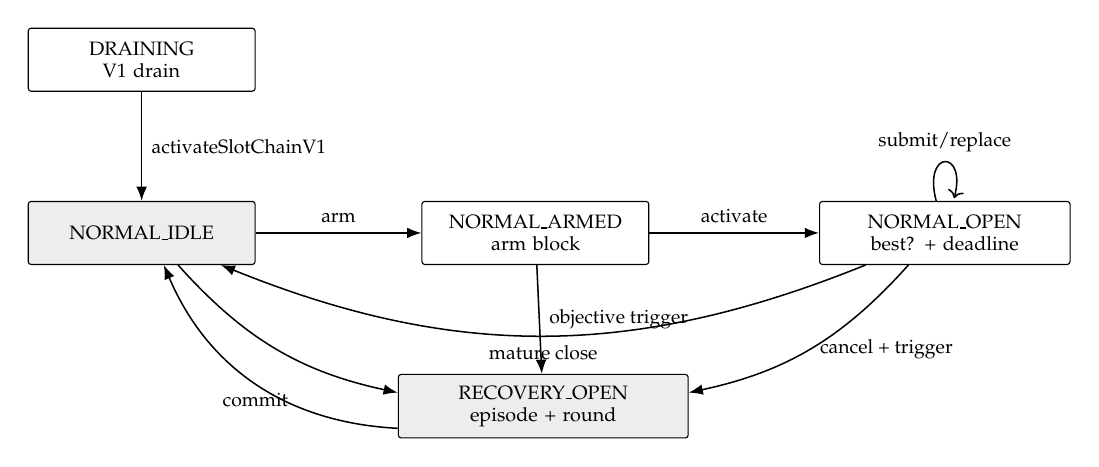
\begin{tikzpicture}
\node[shaded,text width=26mm] (idle) at (0,1.9) {NORMAL\_IDLE};
\node[box,text width=26mm] (armed) at (5.0,1.9) {NORMAL\_ARMED\\arm block};
\node[box,text width=29mm] (open) at (10.2,1.9) {NORMAL\_OPEN\\best? + deadline};
\node[shaded,text width=34mm] (recovery) at (5.1,-0.3) {RECOVERY\_OPEN\\episode + round};
\node[box,text width=26mm] (draining) at (0,4.1) {DRAINING\\V1 drain};
\draw[arrow] (draining) -- node[right,font=\scriptsize]{activateSlotChainV1} (idle);
\draw[arrow] (idle) -- node[above,font=\scriptsize]{arm} (armed);
\draw[arrow] (armed) -- node[above,font=\scriptsize]{activate} (open);
\draw[arrow] (open) edge[loop above] node[above,font=\scriptsize]{submit/replace} (open);
\draw[arrow] (open) to[bend left=22]
  node[below,font=\scriptsize]{mature close} (idle);
\draw[arrow] (idle) to[bend right=18] (recovery);
\draw[arrow] (armed) -- node[right,font=\scriptsize]{objective trigger} (recovery);
\draw[arrow] (open) to[bend left=18] node[right,font=\scriptsize]{cancel + trigger} (recovery);
\draw[arrow] (recovery) to[bend left=32]
  node[below,font=\scriptsize]{commit} (idle);
\end{tikzpicture}
\caption{The complete mode machine.  DRAINING is entered once at install and
left once at activation (\S\ref{sec:upgrade}); no later transition returns to
it.  Payments are outside every arrow.}
\end{figure}

\subsection{Normal context and candidates}

Normal context creation is two-phase.  Anyone calls \code{armNormalContext()}
in \code{NORMAL\_IDLE}; the call begins with \code{sync()}, stores only
\code{armBlockNumber=block.number}, and emits \code{NormalContextArmed}.  It
accepts no caller-supplied anchor or hash.  In a later L1 block anyone calls
\code{activateNormalContext()}.  It again begins with \code{sync()} and requires
the arm's block-number age to be from 1 through
\code{MAX_ARM_AGE_BLOCKS} (255),
reads \code{armBlockHash=blockhash(armBlockNumber)}, and hashes a supplied RLP
header to that value.  It then freezes \code{baseCanonical},
\code{deadline=block.timestamp+W_SETTLE_SECONDS},
\code{minAdmissibleSlot=max(0,currentL2Slot-DELTA_TIP)}, the current stable
\code{(admissionVersion,admissionRoot)}, the arm header fields, and
\code{requiredThrough=deadline+T_INCLUDE_MAX_SECONDS}.  It derives the sole
normal \code{contextId} and emits \code{NormalContextActivated}.  No candidate
is accepted while armed.  If age exceeds 255 blocks, any caller may invoke
\code{armNormalContext()} again; after its leading \code{sync()} it atomically
replaces only the stale arm number with the current block, emits
\code{NormalContextRearmed}, and returns \code{REARMED}.  A nonstale arm cannot
be replaced.  Thus an abandoned arm cannot suppress normal operation.

Builders collect and issue tier-1 signatures only after the activation event.
The execution anchor for every candidate is the exact arm block, whose hash and
parsed header are already frozen; replacements hash their supplied RLP header
to that stored hash and never repeat an EIP-2935 recency lookup.  Every block
of the candidate carries that arm block hash in its header
\code{parentBeaconBlockRoot} (\S\ref{sec:blocks}); no anchor transaction
exists.  A reorg that
removes the arm block necessarily changes the context.  If the arm block
survives but the activation transaction is reorged, reactivation intentionally
recreates the same context: the builder must retain and honor its prior
same-context signature.  Evidence compares the exact common anchor/force tuple
and treats this derived context ID as the signed promise namespace; it does not
need activation storage or an EIP-2935 lookup after the builder has produced
both signatures.  Thus a shallow reorg cannot erase culpability, and an
attacker cannot choose an anchor without the builder signing both conflicting
registered-domain headers.

Activation is permissionless, reserves no builder, and does not block
submissions.  An empty activated window merely cancels at deadline, so an
opener gains no censorship right.  Every candidate first
proves its frozen-prefix boundary in the circuit.  It also supplies a canonical
single-leaf Merkle proof at \code{endCursor} under the queue's current
root/count, or proves \code{endCursor==currentCount}.  Settlement verifies the
canonical depth-64 singleton proof, which contains exactly 64 sibling hashes,
and requires the resulting
\code{currentBoundaryDueAt} to exceed
\code{requiredThrough}.  This prevents an old but valid anchor from hiding a
post-anchor append.  Because due times are monotone, one current boundary leaf
proves that every item due through the landing horizon is consumed.  Later
candidates use the same base, deadline, minimum, admission pair and horizon.
Their total order is lexicographic:

\[
(\text{block count descending},\ \text{tip slot descending},\
 \text{tip hash ascending}).
\]

Only a strictly better candidate replaces \code{normalBest}; the stored best
contains \code{endCursor} and the minimum expiry of every referenced data
session.  Provisional replacement changes no canonical state and pays nobody.
At or after the deadline, \code{sync()} reads
\code{ForcedQueue.dueAt(best.endCursor)} and commits only if that live boundary
is greater than \code{block.timestamp} and
\code{block.timestamp+REORG_MARGIN_SECONDS <= best.minDataExpiry}.  A commit
is the canonical commit of \S\ref{sec:canonical-commit}.  Thus a late
close cancels rather than committing a block that omits an already-due head,
even beyond the assumed inclusion bound, or whose authenticated data has
passed its resubmission margin.  Data-session GC cannot evict a session
referenced by the stored best; its own leading \code{sync()} clears an expired
best first.  Because
\code{FORCE_DELAY >= W_SETTLE_SECONDS + T_INCLUDE_MAX_SECONDS}, an append after
open cannot violate the frozen acceptance horizon.  Settlement then recomputes
recovery causes against the new core.

\subsection{Activation}

While normal, \code{sync()} opens one persistent recovery episode if either:

\begin{itemize}
\item \code{currentL2Slot > canonical.tipSlot + DELTA_FINAL_LAG}; or
\item the forced queue's stored \code{dueAt[canonical.messageCursor]} is no
greater than \code{block.timestamp}.
\end{itemize}

A due forced head has precedence over an immature normal window, which is
canceled.  At a mature deadline, a best that consumes the required due prefix
commits before causes are recomputed; an omitting best is canceled.  No best is
promoted across activation.  The contract increments \code{episode}, records
causes and the base-canonical hash, then runs the bounded seat-duty pass in
\S\ref{sec:seat-market}: an objectively missed primary duty is allocated,
failed over or marked breached as applicable, while a full duty ring fails open
to economic vacancy.  This path performs no Market call, bond movement or token
transfer.  Breach enforcement and bond terminalization are later permissionless
noncanonical operations against the retained exact receipt; force-only recovery
creates no aggregator penalty.

Every round freezes \code{roundStartSlot}, the preceding L1 block number/hash,
current \code{forceRoot/forceCutoff}, current
\code{(admissionVersion,admissionRoot)},
and
\code{escapeSlot=max(roundStartSlot+ESCAPE_OFFSET,canonical.tipSlot+1)}.
Its \code{expiresAt} is the checked
\code{GENESIS_TIMESTAMP+escapeSlot+DELTA_TIP} and round creation or renewal
requires the result to be strictly less than \code{UINT64_MAX}.  A terminal
value cannot support a representable forced-message deadline strictly after the
round and is therefore rejected rather than saturated or wrapped.  The frozen
L1 hash is the round anchor: every block of a recovery candidate, signed or
escape, carries it in its header \code{parentBeaconBlockRoot}, which is how it
reaches the L2 beacon-roots ring (\S\ref{sec:bridge}); nothing else
publishes it on L2.  The exact ID is:
\begin{verbatim}
recoveryId = H("slot-chain-recovery-v2",
               u256(settlementChainId), address20(contract),
               u64(episode), u64(revision), bytes32(baseCanonicalHash),
               u64(roundStartSlot), u64(anchorNumber), bytes32(anchorHash),
               bytes32(forceRoot), u64(forceCutoff), u64(admissionVersion),
               bytes32(admissionRoot), u64(escapeSlot), u8(causes))
\end{verbatim}
At \code{block.timestamp > expiresAt}, and never before, \code{sync()} replaces
the expired target with revision $r+1$ and fresh round fields, then returns
\code{SYNCED}.  It does not change episode/base/cause, create another duty,
promote, terminalize a bond or pay.  The old proof is already inadmissible, so permissionless
refresh cannot grief a still-live proof.  New queue appends enter the refreshed
cutoff.  An envelope admitted during recovery receives the exact
Settlement-derived SIF1 floor \code{currentRound.expiresAt+1}, and hence
\code{dueAt=max(enqueuedAt+FORCE_DELAY,lastDueAt,currentRound.expiresAt+1)};
therefore it
cannot become due while a frozen round that omits it remains admissible.

\subsection{Recovery acceptance}

Recovery is first-valid, not heaviest.  A tier-2 or tier-3 candidate \must:

\begin{enumerate}
\item extend the exact current stored canonical state;
\item bind current \code{episode}, \code{revision}, \code{recoveryId}, frozen
admission pair, anchor and queue target;
\item land at least \code{F_L1} L1 blocks after its anchor, have first slot
at least \code{roundStartSlot}, tip no older than
\code{DELTA_TIP}, and no slot later than wall clock plus skew;
\item consume the exact maximum forced-message prefix from the current cursor,
bounded by the current round's frozen cutoff; and
\item satisfy its tier-specific signature/data restrictions and validity proof.
\end{enumerate}

A tier-3 escape candidate is exactly one block containing only that forced
prefix, which may be empty.  An empty escape block has no transactions at all;
it still advances the canonical tip, carries the round anchor hash in
\code{parentBeaconBlockRoot} and expires every omitted promise
(\S\ref{sec:blocks}).

The first valid L1 transaction performs the canonical commit below, records the
current L1 block \emph{number only} as \code{canonicalizedAtBlock}, clears the
recovery episode and returns to normal.
Later proofs are stale.  Candidate rejection cannot undo activation because of
the early-return wrapper in \S\ref{sec:state}.

\subsection{Canonical commit}\label{sec:canonical-commit}

Exactly three transitions write \code{Canonical}: the mature normal close
inside \code{sync()}, a recovery-signed commit and an escape commit.  Each is
one internal transition in one revert domain that
\begin{enumerate}
\item compares every base field with storage, verifies the proof, writes the
proved \code{CanonicalCore} and then \code{canonicalizedAtBlock=block.number}
(\S\ref{sec:state});
\item calls \code{ForcedQueue.advanceCursor(start,end,proofBeneficiary)}
exactly once for the consumed prefix
\code{[canonical.messageCursor, endCursor)}, with \code{start=end} when that
prefix is empty (\S\ref{sec:escape});
\item calls the L1 SignalService's
\code{saveCheckpoint((uint48(l2BlockNumber), tipHash, stateRoot))}
exactly once; the call \must{} succeed, and a revert rolls back the whole commit
(\S\ref{sec:bridge}); and
\item emits the canonical event \code{(l2BlockNumber, tipHash, stateRoot)}.
\end{enumerate}
Those two calls are the only external calls in the commit path; neither is
skipped, deferred or caller-optional, and no other path calls
\code{saveCheckpoint}.  The only other writer of \code{Canonical} is the
one-time activation import of \S\ref{sec:upgrade}, which imports the V1 tip
and emits the same event.  A provisional replacement of \code{normalBest}, a
round renewal and a canceled window write no canonical state and make neither
call.  In the same transaction, after the commit, Settlement recomputes
recovery causes, runs the bounded seat-duty pass (\S\ref{sec:seat-market}) and
records the optional reward receipt (\S\ref{sec:economics}); none of those
can revert the commit.

\clearpage
\section{Forced queue and unsigned escape}\label{sec:escape}

This section specifies the single censorship-resistant ingress lane of the
protocol: the L1 \code{ForcedQueue}, its one payable entry point, the
per-block forced prefix that every proved block \must{} consume, the
proof-internal classification of forced items, and the unsigned escape block
that drains the queue when no builder or aggregator acts.  There is exactly
one forced kind.  \code{ForcedKind} has the single member
\code{0=USER_TRANSACTION}; value 1 is unassigned and rejects everywhere.
There is no bridge-credit kind, no protocol system transaction, no separate
ingress adapter or router, and no second ingress path: every forced item is
an ordinary signed L2 transaction submitted by its own sender.  Bridging in
both directions uses the existing SignalService and Bridge contracts and
needs no forced kind of its own; a user censored on L2 force-includes an
ordinary \code{Bridge.processMessage} transaction through this queue.
Ownership, upgrades and deployment of the queue follow the common rules in
\S\ref{sec:governance}.

\subsection{Forced envelope and admission}\label{sec:forced-envelope}

\code{ForcedEnvelope} (kind 0) is
\code{(sender,nonce,l2ChainId,rawTxHash,byteLength,gasLimit,maxFee,validUntil,
refundAddress,deposit)}.  Every field except \code{validUntil},
\code{refundAddress} and \code{deposit} is derived by the queue from the raw
transaction bytes; no duplicated caller field or caller hash is
authoritative.  The sole entry, a function of the \code{ForcedQueue} contract
itself, is
\begin{verbatim}
enqueueForcedTransactionV2(bytes rawTransaction, uint64 validUntil,
                           address refundAddress)
  payable returns (uint8 result, uint64 queueIndex)
// selector 0x9f06b1b4
\end{verbatim}
The selector is the first four Keccak bytes of
\code{"enqueueForcedTransactionV2(bytes,uint64,address)"}.  Word 0 is the
canonical bytes offset \code{0x60}, word 1 the canonically padded validity
deadline and word 2 the canonically padded nonzero refund address.  The tail
is one length word, the nonempty raw EIP-2718 bytes and zero right-padding;
total calldata length is exactly \code{132+ceil32(rawTransaction.length)}
bytes.  The queue re-encodes and byte-compares the complete call before any
state read or write, so aliases, gaps, overlap, trailing bytes, dirty padding
or nonzero right-padding reject.  There is no relayed entry: \code{msg.sender}
\must{} equal the recovered transaction signer, and any future EIP-712 relay
requires a new function and codec.  The return is exactly 64 bytes: result
\code{QUEUED=1} in word 0 and the new queue index in word 1.  No other result
value is ever returned; every failure reverts, so a non-append never retains
value, queue state or an event.

From the exact raw bytes the queue recovers the sender and derives nonce,
chain ID, raw transaction hash (legacy Keccak-256 of the signed EIP-2718
bytes), raw byte length, intrinsic gas, gas limit and maximum fee per gas.
The transaction chain ID \must{} equal the queue's immutable \code{l2ChainId}.
Only EIP-155 chain-protected legacy transactions (type 0), EIP-2930
access-list transactions (type 1) and EIP-1559 dynamic-fee transactions
(type 2) are admitted, and each only when enabled by the L2 fork in force.
Unprotected legacy, blob type 3, authorization-list type 4, type \code{0x7f}
and every unknown type reject at admission.  This restriction is on the
forced lane; discretionary transaction support follows the L2 fork.
Admission validates the complete canonical transaction grammar, signature,
chain ID, supported type, nonce below \code{UINT64_MAX}, fee-field relations,
checked upfront cost and fork-specific creation limits.  In particular,
\code{gasLimit >= max(intrinsicGas,calldataFloorGas)} is mandatory; the
capacity charge \code{accountedGas} of \S\ref{sec:forced-fees} cannot make an
invalid transaction valid.  Intrinsic gas includes access-list and
contract-creation charges and the EIP-3860 initcode-word charge where active;
calldata floor gas is \code{21000+10*(zeroBytes+4*nonzeroBytes)} where
EIP-7623 is active and zero otherwise.  EIP-3860 bounds initcode to 49,152
bytes where active.  Fee caps and \code{value+gasLimit*maxFee} \must{} fit
\code{uint256}; a type-2 priority fee cannot exceed its maximum fee.
Legacy/type-1 fields cannot carry type-2-only data.  The L2 fork's
transaction gas cap also applies where active.  The admission grammar is
fixed by the \code{ForcedQueue} implementation for the L2 fork in force and
is never taken from caller-provided validity flags; an L2 fork that changes
the grammar requires a queue implementation upgrade (\S\ref{sec:governance})
before its activation.  Execution witnesses reconstruct these facts from the
committed raw bytes and the proved L2 prestate, not from caller-authoritative
descriptor fields.

Admission further requires \code{0<byteLength<=131,072},
\code{0<accountedGas<=MAX_FORCE_MESSAGE_GAS=5,000,000}, a nonzero
\code{refundAddress}, an unexpired deadline
\code{validUntil>=block.timestamp} and
\code{validUntil<=enqueuedAt+MAX_FORCE_VALIDITY_SECONDS}.  The validity
horizon is seven days (604,800 s).  Every failure reverts before any ETH is
retained or any queue state is written.

The durable descriptor is the fixed-width 220-byte
\code{Kind0ForcedDescriptorV2}; the corresponding admission body
\code{Kind0ForcedAdmissionV2} is the same sequence with the adjacent
\code{u64(enqueuedAt)||u64(dueAt)} removed, hence exactly 204 bytes.  Its
schema identity is \code{H("slot-chain-force-user-admission-v2")}.  The
queue forms the admission body from the decoded transaction, inserts the two
live timestamp words computed in \S\ref{sec:forced-fees} immediately before
the final \code{u256(deposit)}, and stores only the resulting durable body.
No zero placeholder, caller timestamp or alternative field order is a valid
leaf preimage.  Forced leaf $i$ is legacy Keccak over
\begin{verbatim}
"slot-chain-force-user-v2" || u64(i) ||
address20(sender) || u64(nonce) || u256(l2ChainId) || bytes32(rawTxHash) ||
u32(byteLength) || u64(gasLimit) || u64(accountedGas) ||
u256(maxFee) || u64(validUntil) || address20(refundAddress) ||
u64(enqueuedAt) || u64(dueAt) || u256(deposit)
\end{verbatim}
exactly as fixed in Appendix~\ref{sec:encodings}.  The descriptor schema of
the queue is
\begin{verbatim}
descriptorSchemaHash = H("slot-chain-force-descriptor-schema-v12")
  = 0xba2d2a183add1532d454fedbdbb88f382ba69738e1c6bf9e4c68028515f5c4c5
\end{verbatim}
and covers the kind-0 body only.  The kind-0 leaf, descriptor and
classification decoders are protocol-lifetime queue ABIs: every future L2
fork and every future queue implementation \must{} retain their exact
semantics for all entries below \code{count}; a later version may add a new
tagged kind but cannot reinterpret an existing byte.  The mandatory codec
corpus pins raw-transaction lengths of 0 (rejected), 31, 32, 33 and 131,072
bytes and rejects a one-byte mismatch between the raw bytes, the descriptor,
the fee and the per-block byte accounting.

\subsection{Fees and due time}\label{sec:forced-fees}

The capacity charge is
\code{accountedGas=max(gasLimit,intrinsicGas,MIN_FORCE_ACCOUNTED_GAS)} with
\code{MIN_FORCE_ACCOUNTED_GAS=21,000}, and \mustnot{} exceed
\code{MAX_FORCE_MESSAGE_GAS=5,000,000}.  That constant bounds only
\code{accountedGas}; it is not a separate transaction gas limit, although a
transaction whose own \code{gasLimit} exceeds it necessarily rejects.  The
queue implementation fixes one five-word fee schedule
\begin{verbatim}
(fixedIngressWei, executionWeiPerAccountedGas,
 proofWeiPerAccountedGas, permanentWeiPerByte,
 maximumAcceptedFeeWei).
requiredDeposit = fixedIngressWei
  + accountedGas * (executionWeiPerAccountedGas
                    + proofWeiPerAccountedGas)
  + byteLength * permanentWeiPerByte.
\end{verbatim}
All additions and multiplications are checked \code{uint256}; every
coefficient and the cap is nonzero,
\code{requiredDeposit<=maximumAcceptedFeeWei}, and an implementation is
invalid unless the maximum gas/byte geometry and
\code{UINT64_MAX*maximumAcceptedFeeWei} are representable.  The entry
requires \code{msg.value=descriptor.deposit=requiredDeposit} exactly;
overpayment and underpayment both revert before retained state.
\code{fixedIngressWei} is the calibrated upper bound for all admission costs
independent of \code{accountedGas} and \code{byteLength}, including the fixed
descriptor, event, cold-account and fixed storage-write geometry.
\code{executionWeiPerAccountedGas}, \code{proofWeiPerAccountedGas} and
\code{permanentWeiPerByte} are respectively upper bounds, with an explicit
safety margin, for execution gas, proving cost and permanent
publication/storage of one raw input byte.  The release records the L1
base-fee, blob-fee and L2/prover price caps and margin used to derive all
four amounts; a release whose benchmark corpus exceeds any bound rejects.
The deposit is deliberately nonrefundable after append: it buys FIFO
storage, proving and processing even when an expired or invalid item has no
Ethereum transaction.  \code{refundAddress} remains part of the descriptor
for transaction-level compatibility but creates no queue-fee entitlement in
this version; changing consumption or payment requires changing the
descriptor and the proof statement.

Due time depends on the Settlement's ingress floor.  Before computing it the
queue makes one zero-value \code{STATICCALL} to its immutable
\code{settlement} address (the Inbox proxy):
\begin{verbatim}
settlementForcedIngressFloorV1() returns
 (bytes4 magic,uint64 minimumDueAt)
// selector 0xfe2a2914; calldata exactly 4 bytes; exact 64-byte return;
// magic SIF1=0x53494631; exact STATICCALL gas 50,000; value zero
\end{verbatim}
\code{minimumDueAt=0} if and only if canonical mode is NORMAL.  In RECOVERY
it is the checked value \code{currentRound.expiresAt+1}.  The view derives
this value directly from canonical mode and the exact current round; it
reverts before Slot Chain activation and for any conflicting mode/round
tuple.  Recovery-round creation and roll require \code{expiresAt<UINT64_MAX};
they never saturate or wrap.  The queue rejects revert, out-of-gas, short or
trailing return data, bad magic or dirty \code{uint64} padding.
Consequently no item can be enqueued before the Settlement has activated
Slot Chain, and \code{ForcedQueue.count=0} at activation.

Only after the SIF1 read succeeds does the queue compute
\code{enqueuedAt=block.timestamp} and
\begin{verbatim}
dueAt = max(enqueuedAt + FORCE_DELAY, lastDueAt, minimumDueAt)
\end{verbatim}
using checked \code{uint64} addition for the first term, and appends
atomically.  Thus \code{block.timestamp=UINT64_MAX-FORCE_DELAY} remains
admissible with base due time \code{UINT64_MAX}, while the next timestamp
rejects before any state write.  Neither an enqueue timestamp nor a due time
is accepted in calldata.  At equality with a live recovery expiry SIF1 is
already one second later, so an item appended after a round's cutoff was
frozen cannot become due while that round's proof remains admissible; an
item appended after the round has expired but before \code{sync()} rolls it
lies below the refreshed cutoff, because refresh freezes the live count.
Hence no frozen admissible recovery proof can omit an item that has become
due, and because
\code{FORCE_DELAY >= W_SETTLE_SECONDS + T_INCLUDE_MAX_SECONDS} an append
after a normal window opens cannot violate its frozen acceptance horizon
(\S\ref{sec:machine}).  \code{dueAt} is nondecreasing in queue index.

\subsection{ForcedQueue contract}\label{sec:forced-queue-contract}

\code{ForcedQueue} is one L1 contract deployed as a DAO-owned proxy with the
storage-layout, reinitializer and owner-only-upgrade rules of
\S\ref{sec:governance}.  Its implementation pins as constructor immutables
the Settlement address \code{settlement} (the existing Inbox proxy),
\code{l2ChainId}, \code{FORCE_DELAY}, \code{MAX_FORCE_VALIDITY_SECONDS}, the
three geometry constants \code{MAX_FORCE_MESSAGE_GAS=5,000,000},
\code{MAX_FORCE_MESSAGE_BYTES=131,072} and
\code{MIN_FORCE_ACCOUNTED_GAS=21,000}, and the five fee-schedule words.  No
initializer, setter or storage slot supplies any of them; changing one is a
governance upgrade of the implementation.  The one-shot initializer installs
the canonical empty root and zero count, cursor, last due time, deposit
prefix, escrow and claim liabilities.  No queue entry point is pause-gated:
pausing enqueue would be a censorship vector, pausing \code{advanceCursor}
would halt canonical commits, and pausing withdrawal would trap earned
credits.  The deployment view is
\begin{verbatim}
forcedQueueConfigV1() returns
 (bytes4 magic,address settlement,uint256 l2ChainId,
  uint8 depth,uint64 capacity,bytes32 emptyLeaf,
  bytes32 descriptorSchemaHash,
  uint64 forceDelay,uint64 maxForceValiditySeconds,
  uint64 maxForceMessageGas,uint32 maxForceMessageBytes,
  uint64 minForceAccountedGas,
  uint256 fixedIngressWei,uint256 executionWeiPerAccountedGas,
  uint256 proofWeiPerAccountedGas,uint256 permanentWeiPerByte,
  uint256 maximumAcceptedFeeWei,bytes32 configurationHash)
// selector 0x8136fe31; exact 576 bytes; magic FQC1=0x46514331
\end{verbatim}
with \code{depth=64}, \code{capacity=UINT64_MAX} and
\code{emptyLeaf=H("slot-chain-force-empty-v2")}.  Its configuration
commitment is
\begin{verbatim}
queueConfigBytes = address20(settlement) || u256(l2ChainId) || u8(64) ||
  u64(UINT64_MAX) || H("slot-chain-force-empty-v2") ||
  descriptorSchemaHash || u64(FORCE_DELAY) ||
  u64(MAX_FORCE_VALIDITY_SECONDS) || u64(5000000) || u32(131072) ||
  u64(21000) || u256(fixedIngressWei) ||
  u256(executionWeiPerAccountedGas) || u256(proofWeiPerAccountedGas) ||
  u256(permanentWeiPerByte) || u256(maximumAcceptedFeeWei)
forcedQueueConfigHash =
  H("slot-chain-forced-queue-config-v2" || u16(321) || queueConfigBytes)
\end{verbatim}
and \must{} equal the \code{componentConfigHashV2()} result (selector
\code{0xf6c0f7d2}, exactly 32 return bytes) byte for byte.  The Merkle
constants (empty leaf, node domain and wrapped root) are fixed in
Appendix~\ref{sec:encodings}.

Only the queue's own enqueue path appends.  The internal append receives the
204-byte admission body, the live \code{enqueuedAt} and the computed
\code{dueAt}; it requires the canonical field rules of
\S\ref{sec:forced-envelope}, \code{dueAt>=enqueuedAt},
\code{dueAt>=lastDueAt}, \code{count<UINT64_MAX} and
\code{msg.value=deposit>0}, and then writes the descriptor,
\code{depositPrefix[count+1]=depositPrefix[count]+deposit} (checked), the
append frontier, root, count, \code{lastDueAt}, the escrow liability and the
event together, or reverts together.  No external account is called on this
path after the SIF1 read.  The queue stores one authoritative
\code{QueueDescriptor} per index: the complete 220-byte durable body, which
excludes only the raw transaction bytes themselves but includes their hash.
Thus sender, nonce, chain ID, byte/gas fields, fee, validity, refund
address, enqueue/due times and deposit remain durable.  The Merkle leaf is
always recomputed from this stored descriptor.  The queue is also the sole
owner of \code{cursor}; the Settlement has no second descriptor array, root,
count, cursor or due-time cache.

The exact read surface is
\begin{verbatim}
forcedQueueStateV1() returns
 (bytes4 magic,address settlement,bytes32 root,
  uint64 count,uint64 cursor,uint64 lastDueAt,
  uint256 unconsumedEscrow,uint256 totalClaimable,
  uint256 accountedLiability,bytes32 configurationHash)
// selector 0x03e0d70b; exact 320 bytes; magic FQS1=0x46515331

forcedQueueFrontierV1() returns
 (bytes4 magic,uint64 count,bytes32 root,bytes32[64] frontier)
// selector 0x7c339ff7; exact 2,144 bytes; magic FQF1=0x46514631

forcedQueueDescriptorV1(uint64 index) returns
 (bytes4 magic,uint64 returnedIndex,uint8 kind,bytes descriptorBytes)
// selector 0xbd9534db; exact 384 bytes; magic FQD1=0x46514431

dueAt(uint64 index) returns (uint64 returnedDueAt)
// selector 0x530fd138; calldata 36 bytes; exact 32-byte return
\end{verbatim}
FQS1 and FQF1 recompute no history.  FQF1 returns the stored 64-word
frontier; only set-bit words are semantically live.  FQD1 requires
\code{index<count}, returns \code and exactly the stored 220-byte
body (zero-padded to 224), and otherwise reverts.  \code{dueAt} instead
returns \code{UINT64_MAX} for every missing index.  Because that value is
also a valid deadline, every force-due or live-boundary decision first
requires \code{cursor<count}; only then may it compare \code{dueAt(cursor)}
to the timestamp.  A consumed or absent boundary is never due, including at
timestamp \code{UINT64_MAX}; a present final boundary whose stored deadline
is exactly \code{UINT64_MAX} becomes due at equality.  Force-due and
coverage checks are therefore one authoritative O(1) read with one O(1)
existence check.  FQC1, FQS1, FQD1 and \code{dueAt} use respectively 50,000,
100,000, 100,000 and 50,000 gas; FQF1 uses 300,000.  All direct consumers
enforce exact calldata, return length, magic and narrow-word padding.

The single cursor transition is
\begin{verbatim}
advanceCursor(uint64 expectedStart,uint64 end,
              address proofBeneficiary) returns
 (bytes4 magic,uint64 oldCursor,uint64 newCursor,uint256 creditedWei)
// selector 0xd59ff200; exact 128 bytes; magic FCA1=0x46434131
\end{verbatim}
It is callable only by \code{settlement}; any other caller reverts.  It
requires \code{cursor=expectedStart<=end<=count}, writes the cursor and, in
O(1), moves \code{depositPrefix[end]-depositPrefix[expectedStart]} from
unconsumed escrow to \code{claimable[proofBeneficiary]}.  The beneficiary is
the exact nonzero public input authenticated by the accepted proof; it is
not chosen by the queue caller.  The queue remains the ETH custodian and
enforces the solvency lower bound
\code{address(this).balance >= unconsumedEscrow+totalClaimable}; every
claim-ledger mutation updates \code{totalClaimable} by the same checked
amount, so no global sum or scan is performed.  ETH forced into the contract
without an append is surplus, never enters either liability and cannot make
an append, advance or withdrawal revert.  There is no per-item callback and
no ``unused'' refund.

The unpausable CEI pull-withdrawal ABI is
\begin{verbatim}
withdrawForcedQueueClaimV1(address recipient) returns
 (bytes4 magic,uint256 amount)
// selector 0xc28aa0e8; exact 64 bytes; magic FQW1=0x46515731
\end{verbatim}
The claimant is always \code{msg.sender}; recipient \must{} be nonzero and a
zero claim rejects.  It zeros the claimant's credit and decrements
\code{totalClaimable} before one non-reentrant value transfer.  A failed or
reentrant transfer restores the claim and cannot affect another claimant.

The queue's complete event ABI is
\begin{verbatim}
event ForcedQueueAppended(
 uint64 indexed queueIndex,uint8 indexed kind,bytes32 leaf,
 bytes32 root,uint64 count,uint64 dueAt,uint256 deposit);
event ForcedQueueCursorAdvanced(
 uint64 indexed oldCursor,uint64 indexed newCursor,
 address indexed proofBeneficiary,uint256 creditedWei);
event ForcedQueueClaimWithdrawn(
 address indexed claimant,address indexed recipient,uint256 amount);
\end{verbatim}
\code{kind} is always 0.  The permanent descriptor getter plus the append
leaf/root event is sufficient to reconstruct and verify historical frontier
changes without treating logs as authority.

The queue is a protocol-lifetime, depth-64 append-only Merkle vector with
fixed capacity \code{UINT64_MAX} items: the final leaf is deliberately
unused.  It stores root, \code{uint64} count/cursor, cumulative deposit
prefix and a 64-node append frontier.  Admission rejects only when
\code{count=UINT64_MAX}; no upgrade rotates or resizes the queue.  A
canonical DFS range multiproof authenticates the consumed leaves and, when
present, the first excluded boundary leaf under the frozen
\code{(forceRoot,forceCutoff)}.  It supplies no fully covered subtree and no
unused hash; at most 257 sibling hashes authenticate a 65-leaf block range.
Skipping, reordering, changing the start index or claiming an early boundary
changes the reconstructed root.  Raw transaction bytes are enqueue calldata
and their hash is in the leaf; blobs are forbidden on this availability
path.  The deliberately unused final tree leaf avoids a nonexistent
height-64 frontier slot when the old index has all 64 bits set.  At one
billion appends per second the usable space lasts more than five centuries,
so exhaustion is outside any credible Ethereum lifetime while remaining an
explicit hard stop.

\subsection{Per-block prefix and block composition}\label{sec:forced-prefix}

Each proved block consumes the unique maximum FIFO prefix of the frozen
queue, starting at the block's cursor, that satisfies all three per-block
bounds simultaneously:
\[
count\le64,\qquad \sum byteLength\le1{,}048{,}576,\qquad
\sum accountedGas\le forceGasBudget=20{,}000{,}000 .
\]
There is one steady budget for every block; no activation or first-block
budget exists.  Every admitted item individually fits all three, so the due
FIFO head is always admissible.  The circuit exposes
\code{(start,end,count,totalBytes,totalAccountedGas,forceRoot,forceCutoff,
nextDueAt,forceGasBudget)} per block and verifies the range multiproof.
Maximality means either \code{end=forceCutoff}, or the authenticated next
leaf would exceed at least one remaining per-block cap; an early stop with a
fitting leaf rejects.  Candidate totals are independently capped at 256
items, 4 MiB and 80,000,000 accounted gas as stated in \S\ref{sec:blocks}.
The steady block gas inequality (20,000,000 forced plus 5,000,000 margin
under the 30,000,000 block limit) and the analogous witness-byte bounds are
enforced in \S\ref{sec:implementation}.  Cutoffs do not change within a
candidate: the first blocks drain the frozen prefix and later blocks see an
empty prefix.

For the candidate's exact consumed interval, Settlement reads at most 256
descriptors plus the first excluded boundary descriptor when one exists
under the frozen cutoff; internal per-block boundaries are already the next
consumed descriptor.  It computes
\begin{verbatim}
H("slot-chain-force-descriptor-list-v2" || u64(start) ||
  u16(consumedCount) || u8(hasBoundary) ||
  (u64(index)||u8(kind)||u16(descriptorByteLength)||descriptorBytes)*)
\end{verbatim}
as \code{forcedDescriptorCommitment}.  The number of rows is the consumed
count plus the zero-or-one boundary and is at most 257.  Every row has
\code and \code{descriptorByteLength=220}; \code{descriptorBytes} is
exactly the leaf sequence beginning immediately after \code{u64(i)}, so
neither the leaf ASCII domain nor the index is duplicated inside it.  Row
indices are the contiguous sequence \code{start+i}, checked in 64 bits, and
the boundary, when present, is exactly \code{start+consumedCount}.  The
circuit reconstructs every leaf, range proof, per-block maximum, candidate
total and fee transfer from these L1-authenticated descriptors.  It
additionally requires raw bytes for an unexpired item; an expired item needs
neither historical calldata nor any unstored preimage.

Forced envelopes are auxiliary protocol inputs, not blindly copied into the
Ethereum transaction list.  There are no protocol system transactions.  Each
block's transaction list is exactly: (1) the upfront-valid forced
transactions of the block's frozen FIFO prefix, in queue order, then (2) the
discretionary transactions of the signed body.  Items of the prefix whose
classification (\S\ref{sec:forced-classification}) is not
\code{INCLUDED_TX} are consumed without any transaction.  An upfront-valid
item appears as an ordinary Ethereum transaction whose success or revert has
ordinary nonce/gas/receipt semantics.  The circuit derives the transaction
and receipt roots from this exact order.  The full consumed fee interval is
pull-credited to the proof beneficiary by the same L1 canonical commit
(\S\ref{sec:forced-settlement}).

The escape (tier 3) block has no builder signature, no
beneficiary-controlled coinbase, no discretionary transaction and no blob
body.  Its transaction list is exactly the deterministic maximum forced
prefix of the current recovery round's frozen queue under the same three
bounds.  When that prefix is empty the escape block has zero transactions
(an ``empty escape block'').  It still advances the canonical tip, expires
every omitted promise, and carries the round's anchor hash in its header
\code{parentBeaconBlockRoot}, so that the standard EIP-4788 pre-execution
call records a fresh L1 checkpoint on L2; its remaining header fields, slot
and coinbase sink are fixed by \S\ref{sec:blocks} and \S\ref{sec:machine}.
Its block hash and state root are therefore unique functions of the current
recovery round and the proved execution result.  Because an escape block
needs no builder and no aggregator, a builder cartel can neither censor a
due forced item nor stop fresh L1 checkpoints from reaching L2.

\subsection{Total classification}\label{sec:forced-classification}

The proof derives one disposition for every consumed item, sequentially,
under the fork active at that L2 block, in the pre-state that follows all
earlier included forced transactions of the same block.  Dispositions are
circuit-internal: they are neither written to L2 storage nor sent to L1, and
the Settlement learns only the new \code{messageCursor}.  The codes are
fixed:
\begin{verbatim}
0 = EXPIRED_NO_TX   1 = NONCE_NO_TX   2 = FUNDS_NO_TX
3 = FEE_NO_TX       4 = INCLUDED_TX   6 = INVALID_NO_TX
\end{verbatim}
Code 5 is unassigned and rejects.  Classification tests expiry, nonce
mismatch, insufficient funds, insufficient maximum fee, then every remaining
upfront-invalid predicate, in exactly the order \code{0->1->2->3->6->4}; the
first applicable reason wins and only an item that passes every test
receives code 4.  Expiry is strictly \code{block.timestamp>validUntil};
equality remains unexpired.  An expired descriptor requires no raw bytes.
An unexpired one requires its exact hash-matching raw transaction and a
complete validity witness; missing bytes cannot be relabeled INVALID.  After
the expiry, nonce, balance/upfront-cost and base-fee tests, code 6 covers
every other consensus-level transaction rejection, including fork/type
changes, intrinsic or floor gas repricing, creation limits, nonce exhaustion
and sender-code eligibility.  EIP-3607 rejects nonempty sender code except
an exact EIP-7702 delegation designation when that fork is active; an
arbitrary prefix or malformed designation is not an exemption.  No newly
active fork rule may leave an admitted item unclassifiable; unsupported
forks cannot be activated without a complete classifier and conformance
corpus.

Codes 0--3 and 6 consume the queue item without inserting an Ethereum
transaction, changing its sender nonce, or emitting a transaction receipt.
Only an upfront-valid item receives code 4.  Its later EVM REVERT,
exceptional halt or execution out-of-gas remains an included transaction
with ordinary gas, nonce and receipt semantics; these are not reasons to
discard it.  The circuit derives the exact row and, for code 4, the
transaction index and legacy Keccak-256 hash of the raw signed bytes; a
prover-supplied Boolean or choice of code 6 is not evidence of invalidity.
Release tests \must{} execute every rejection class at the FIFO head
followed by a valid item and compare the resulting transaction/receipt roots
in independent execution engines and the circuit, including an
admission-to-execution fork change.

\subsection{Expiry and data availability}\label{sec:forced-availability}

Raw transaction bytes are published once, as L1 enqueue calldata, and are
committed by \code{rawTxHash} in the leaf; the queue stores the descriptor,
not the bytes.  A candidate supplies the raw bytes matching \code{rawTxHash}
while the item is unexpired.  If no party retains those bytes, the head
becomes permissionlessly \code{EXPIRED_NO_TX} strictly after
\code{validUntil}, at most \code{MAX_FORCE_VALIDITY_SECONDS} (seven days)
after enqueue, using only the stored descriptor.  Missing user bytes
therefore never become permanent head-of-line blocking, and an expired item
is provable from the durable descriptor alone.  Because the descriptor is
durable and the decoders are protocol-lifetime, no upgrade can strand an
entry below \code{count}.

\subsection{Settlement interaction}\label{sec:forced-settlement}

The queue and the Settlement are bound by one cursor.  Before proof
acceptance the L1 base invariant is
\code{baseCanonical.messageCursor=ForcedQueue.cursor}, and the statement's
\code{startCursor} equals that value.  The statement's \code{endCursor} is
the candidate's proved end; the new \code{CanonicalCore.messageCursor}
equals it.  After proof verification and inside the same internal transition
that writes \code{Canonical}, the Settlement calls
\code{ForcedQueue.advanceCursor(startCursor,endCursor,proofBeneficiary)}.
That call moves the exact cumulative processing-fee interval to the
beneficiary's pull claim; a failed call reverts the entire canonical commit.
Hence after every canonical commit (normal close, recovery commit and escape
commit) \code{CanonicalCore.messageCursor=ForcedQueue.cursor}.  Activation
imports \code{messageCursor=ForcedQueue.count=0}, since the queue rejects
every enqueue before activation, so the invariant holds inductively from the
first Slot Chain block.  L1 never writes L2 state for this purpose, and no
activation or upgrade may repair, overwrite or select among divergent
cursors; a successor Settlement implementation \must{} preserve the cursor
slot and this transition.

The Settlement reads the queue's \code{dueAt} directly for the canonical
head and for a stored best's live boundary; there is no callback, cached
deadline or duplicated scalar.  While normal, \code{sync()} opens recovery
when \code{cursor<count} and
\code{dueAt(canonical.messageCursor)<=block.timestamp}; a due forced head has
precedence over an immature normal window.  Opening or refreshing recovery
freezes only the current stored \code{(root,count)} as
\code{(forceRoot,forceCutoff)}.  Settlement requires the requested cutoff to
equal the live queue count and may validate the wrapped root by folding the
fixed 64-word append frontier; it never recomputes the root from retained
descriptors.  Full descriptor-history root construction exists only as an
off-chain differential test oracle.  Every normal, recovery or escape
candidate consumes the exact maximum prefix from the current cursor bounded
by its frozen cutoff (\S\ref{sec:machine}); a late normal close that would
omit an already-due head is canceled rather than committed.
\section{Checkpoints and bridge integration}\label{sec:bridge}

Slot-Chain adds no bridge.  Users, vaults and applications keep calling the
deployed \code{Bridge} on either chain, which keeps writing and verifying
signals through the deployed \code{SignalService}, which keeps verifying
storage proofs against checkpoints of the other chain.  The only thing
Slot-Chain changes is how those checkpoints are produced.

\subsection{L2 checkpoints on L1}

Every canonical commit (normal close, recovery commit, escape commit) calls
the L1 SignalService's \code{saveCheckpoint} with
\code{(uint48(l2BlockNumber), tipHash, stateRoot)} inside the same internal
transition that writes \code{Canonical} (\S\ref{sec:state}).  The SignalService
authorizes exactly one syncer, its constructor immutable
\code{_authorizedSyncer}, which on the deployed L1 instance is the Inbox proxy
address; because the Settlement is that proxy's implementation, no change to
the SignalService is required for the write to be accepted.  The path is not
pause-gated.  The write is keyed by L2 block number, is written at most once
per canonical commit, and is never written for a non-canonical candidate.
Consumers of the existing \code{CheckpointSaved} event keep their event model:
the L1 \code{Bridge.processMessage}, the relayer and the bridge UI see the
event on the Settlement's commit transaction instead of on \code{Inbox.prove}.
Because the Settlement address does not change, the existing L2 SignalService's
constructor-pinned remote SignalService and the existing resolver entries stay
valid.

Slot-Chain deliberately does not carry an application-level terminal vector,
a canonical history ring or a separate publication call.  The checkpoint
write is internal, atomic with the commit and impossible to front-run or omit;
the rejected-alternative text of v2.28 against an ``external checkpoint
copier'' therefore no longer applies (\S\ref{app:alternatives}).

\subsection{L1 checkpoints on L2}

Every Slot-Chain L2 block carries \code{parentBeaconBlockRoot = anchorHash}
(\S\ref{sec:blocks}).  The standard EIP-4788 pre-execution call, which the L2
clients already run for every block, stores that value in the canonical
beacon-roots contract at
\code{0x000F3df6D732807Ef1319fB7B8bB8522d0Beac02} under the block's timestamp,
in a ring of \code{HISTORY_BUFFER_LENGTH=8191} timestamp keys.  Anyone then
calls the L2 SignalService's
\begin{verbatim}
revealCheckpoint(uint64 l2Timestamp, bytes headerRlp) // selector 0x6c7d3fdf
\end{verbatim}
which reads the recorded hash for \code{l2Timestamp} from the beacon-roots
contract with the raw 32-byte timestamp calldata, requires
\code{keccak256(headerRlp)} to equal it, strictly decodes the L1 header (state
root is RLP item 3 and must be exactly 32 nonzero bytes; number is item 8 and
must fit \code{uint48} before casting), and persists
\code{Checkpoint(number, hash, stateRoot)} under the SignalService's existing
\code{VERSION=1} checkpoint mapping, emitting the existing
\code{CheckpointSaved} event.  A repeated reveal of an identical checkpoint is
a no-op; a conflicting reveal for an existing number rejects.  That entry
point, its decoder and the L2 deployment of the EIP-4788 and EIP-2935
contracts are part of the baseline protocol (taikoxyz/taiko-mono issue
\#22147) and are used by Slot-Chain unchanged; the L2 SignalService's old
authorized-syncer \code{saveCheckpoint} path is disabled on L2 by that
baseline and is never called by Slot-Chain.  The L2 \code{Bridge}'s
\code{processMessage} then verifies the L1 signal against the revealed
checkpoint with the unchanged \code{HopProof}/\code{LibTrieProof} path.

\paragraph{Reveal window.}  The beacon-roots ring index is
\code{timestamp mod 8191}, so a recorded hash stays readable until a later
block whose timestamp maps to the same index is executed, which cannot happen
earlier than \code{CHECKPOINT_REVEAL_WINDOW_SECONDS = 8191} seconds of wall
time after the recording block.  Relayers \must reveal within that window.  A
revealed checkpoint is permanent, so a missed window only means that a newer
anchor must be revealed instead; because a newer L1 state root proves every
signal an older one proved, no message is ever stranded by a missed reveal.
Slot-Chain also guarantees a fresh revealable anchor exists while L2 produces
blocks: a normal candidate's anchor is its arm block, so the newest canonical
block carries an L1 hash at most
\code{W_SETTLE_SECONDS + T_INCLUDE_MAX_SECONDS + CLOCK_SKEW} old; a recovery
candidate's anchor is its round anchor.  Equal L2 timestamps are impossible
because slots strictly increase, and every block of one candidate records the
same hash, which is harmless.

\paragraph{Liveness floor.}  Publishing a fresh L1 hash on L2 requires only a
canonical block, and an escape block requires no builder, aggregator, seat or
blob session.  A builder cartel therefore cannot stop L1-to-L2 messages; at
worst it delays them until the objective recovery trigger, after which any
prover lands an escape block carrying the round's anchor.  Symmetrically,
every escape commit writes the new L2 state root into the L1 SignalService, so
L2-to-L1 messages need no builder either.  The existing Bridge remains
subject to its own guardian pause, QuotaManager and relayer fee model; those
are unchanged and are not Slot-Chain claims (\S\ref{sec:status}).

\paragraph{Censorship-resistant delivery.}  A user whose \code{processMessage}
or \code{revealCheckpoint} transaction is censored by every builder submits it
as an ordinary kind-0 forced transaction (\S\ref{sec:escape}).  The queue's
due-time rule then forces its inclusion in the next canonical block, signed or
unsigned.  No dedicated bridge lane, credit or liquidity mechanism exists or is
needed for that guarantee.

\subsection{What the reused contracts must satisfy}

The deployed contracts already satisfy every requirement below; they are
restated so that a future change to them is reviewed against Slot-Chain:
\begin{itemize}
\item The L1 SignalService's authorized syncer is the Inbox proxy address and
  \code{saveCheckpoint} rejects zero roots and is not pause-gated.
\item The L2 SignalService's \code{revealCheckpoint} is permissionless,
  reads only the canonical beacon-roots contract, decodes the header strictly
  and is idempotent for identical checkpoints.
\item Both Bridges keep the \code{ISignalService} verification interface and
  the immutable SignalService references they were deployed with; the resolver
  entries for \code{bridge} and \code{signal_service} on both chains are not
  rotated by Slot-Chain.
\item The vaults are untouched.
\end{itemize}

\section{Governance, deployment and upgrades}\label{sec:governance}

\subsection{Ordinary upgradeable contracts}

Every Slot-Chain contract is an ERC-1967 proxy whose implementation follows
the repository's \code{EssentialContract} pattern: UUPS with
\code{_authorizeUpgrade} restricted to the owner, \code{Ownable2Step}, the
pause hooks, and storage starting at slot 251 with 50-slot gaps.  On L1 the
owner is the existing DAO controller; the DAO's own delayed proposal process is
the only protocol change authority.  Pausing may gate only optional
Settlement and Market surfaces (seat offers, data-session opens, reward
funding and claims).  No BuilderRegistry, ScheduleOracle or ForcedQueue entry
point is pause-gated, and candidate submission, recovery activation and
renewal, every canonical commit and its checkpoint write, forced enqueue,
\code{advanceCursor}, pull-credit withdrawals and bond withdrawals are never
pause-gated; a pause therefore cannot stop canonical progress, the lookahead,
forced inclusion or refunds.  There are no new L2 contracts.  The components and
their deployment are:

\begin{center}
\small
\begin{tabular}{p{0.40\linewidth}p{0.52\linewidth}}
\toprule
\textbf{Component} & \textbf{Deployment} \\
\midrule
Settlement & New implementation installed in the existing L1 Inbox proxy
  (\S\ref{sec:upgrade}); the address, and therefore the L1 SignalService's
  authorized syncer, does not change. \\
ForcedQueue & New DAO-owned proxy; pins the Inbox proxy as its Settlement. \\
BuilderRegistry & New DAO-owned proxy; its two lifecycle facets and its
  stateless proof verifier are plain immutable helper contracts pinned by
  constructor immutables of the implementation (\S\ref{sec:schedule}). \\
ScheduleOracle & New DAO-owned proxy; the SSZ multiproof verifier is a plain
  immutable helper. \\
AggregatorSeatMarket & New DAO-owned proxy (\S\ref{sec:seat-market}). \\
Validity verifier & Plain immutable release artifact named by the Settlement
  implementation's constructor (\S\ref{sec:blocks}). \\
SignalService, Bridge, vaults (L1 and L2), Anchor treasury (L2) & Existing
  proxies, unchanged. \\
\bottomrule
\end{tabular}
\end{center}

Every component pins the Inbox proxy address as a constructor immutable and
gates new work on \code{settlementStateV1()} (\S\ref{sec:state}).  Because
that address is permanent, no component ever needs a target rotation, a
version registry or a router.  Constructor immutables of one implementation
(facets, verifiers, the SignalService, the ForcedQueue) are replaced by
installing a new implementation, never by a setter.

\subsection{Protocol versions}

\code{protocolVersion} is an immutable of each Settlement implementation.  It
is a signed field of every builder header, part of every context ID and of
every statement (\S\ref{sec:blocks}), so builder promises, candidates and
proofs produced for version $N$ are invalid under version $N+1$ by
construction.  Installing a new implementation with a greater
\code{protocolVersion} is a version upgrade; installing one with the same
version is a bug fix that \mustnot change any consensus rule, encoding or
profile hash.

A version upgrade \must be accompanied by a reinitializer that, in the
upgrade transaction itself, either imports or terminalizes every piece of live
state of the previous version: the live normal context and best candidate
(cancel, refunding session bonds under \S\ref{sec:data}), the live recovery
episode and round (import or cancel; a cancelled round is renewed from the
same base by the next \code{sync()}), open data sessions, seat duties,
reserves and credits (\S\ref{sec:seat-market}), and reward vaults.  The
successor specification \must state which it does for each.  The canonical
core, the forced-queue cursor binding and the bond ledger are always imported.
Equivocation evidence signed under the predecessor version remains admissible
after the upgrade: the BuilderRegistry records, at the first read that
observes a new \code{protocolVersion} from \code{settlementStateV1()}, the
predecessor version and the L2 slot of the change, and keeps accepting
evidence bound to the predecessor version until every evidence deadline of
windows sealed under it has passed (\S\ref{sec:schedule}).  Tranche
liabilities of those windows are released under the unchanged registry rules.
Storage-layout compatibility between the previous and the new implementation
is verified with the repository's layout tooling before the upgrade
proposal is queued; the Settlement's V1 slots 251--257 are never moved
(\S\ref{sec:upgrade}).

\subsection{Release discipline}

The following are release-process requirements enforced by governance review,
not on-chain capabilities:
\begin{itemize}
\item every implementation, verifier and helper artifact is reproducibly
  built from the pinned normative commit, and its runtime hash, constructor
  arguments and execution profile are published before the proposal is queued;
\item the execution profile of the new implementation is validated against
  every inequality in \S\ref{sec:parameters} by the deployment tooling;
\item the L2 client fork that changes header rules (\S\ref{sec:implementation})
  is released and activated at \code{L2_FORK_TIMESTAMP} before the L1
  activation that first requires it;
\item the drain-and-activate drill of \S\ref{sec:upgrade} has been executed on
  a fork of the production deployment.
\end{itemize}
Slot-Chain removes the v2.28 requirements that components be non-proxy,
ownerless or deterministically deployed; it also removes the corresponding
claim that a defect cannot be patched.  A defect in any Slot-Chain component is
patched by an ordinary upgrade, with the same trust in governance that the
current protocol already has.

\section{Perpetual aggregator seat market}\label{sec:seat-market}

The aggregator market is an optional service and payment layer around the
permissionless proof path.  It has four installed ranks---one primary and three
standbys---and a continuous reverse auction with four shared waiting cells.  It
has no auction epoch or fixed close window.  A healthy funded primary persists
until competitive handover, voluntary exit, its one objective duty, funding
expiry or a terminalizing implementation upgrade.  No seat, operator action,
premium balance or Market call is a precondition for proof submission,
canonical commit, forced recovery, recovery renewal or an implementation
upgrade.

\subsection{Authority, identity and bounded call graph}

Settlement alone owns the installed roster, immutable seat terms and service
intervals, one staged-handover commitment, duties, successor selection,
failover, breach receipts and retained duty history.  Every
canonical transition is bounded, scans at most four seat/duty cells and performs
no external call.  If optional seat state is absent, stale, economically
unmaintained or locally full, Settlement closes the affected economics to
vacancy and continues canonical recovery.

The \code{AggregatorSeatMarket}, a DAO-owned proxy (\S\ref{sec:governance}),
alone owns pending offers, native-ETH SLA bonds, premium custody, reserves and
pull credits.  It has no canonical writer and no upgrade-coordination entry
point.  Its implementation pins exactly one Settlement, the Inbox proxy
address, as a constructor immutable, and the Settlement implementation pins the
Market proxy address.  Because that pair of addresses is permanent, there is no
authorization registry, installation operation, rotation or reverse index: the
append-only authorization rows of v2.28 collapse to one binding ID
(\code{authorizationId} below), derived once at Market initialization and
carried by every record.  A Market call may read Settlement only through a
separately specified bounded \code{STATICCALL}; it checks exact chain,
address, selector, return length and magic.  No caller-supplied authority,
mode, generation, operator, close time or validity Boolean is accepted.

The three Settlement read selectors used by Market are fixed to
\code{0xcf52185b}, \code{0x76d5ecd4} and \code{0x9a649489} for state, term
and duty respectively, each with exactly 100,000 gas.  They are protocol
constants; the Market's configuration hash commits the implementations of
those exact ABIs.

The sole offer-book state read is the no-argument selector
\code{seatMarketTargetStateV1()} with canonical ABI return
\begin{verbatim}
(address target, uint256 settlementChainId, uint64 protocolVersion,
 bytes4 magic, uint8 mode, uint64 seatGeneration)
\end{verbatim}
where \code{target=address(this)} (the Inbox proxy),
\code{magic=0x53454154} (ASCII \code{SEAT}), and \code{mode} is the SST1 mode
word of \S\ref{sec:state}: 0 \code{DRAINING}, 1 \code{NORMAL} or 2
\code{RECOVERY}.  Return length is exactly 192 bytes; address, \code{uint64},
\code{bytes4} and \code{uint8} padding must be canonical.  Market makes a
gas-bounded \code{STATICCALL} to its pinned Settlement and compares
\code{target} and \code{settlementChainId} with its immutables; it does not
check \code{EXTCODEHASH}, which for a proxy commits only the proxy stub.
Revert, OOG, short/trailing data or any mismatch fails closed.
\code{AggregatorSeatMarket.syncSeatGenerationV1()} returns exactly
\code{(bytes4 MSG1,uint8 result,uint8 purgedCount,uint8 targetMode,
uint64 generation)} as five ABI words,
where result is UNCHANGED=0 or SYNCED=1 and \code{purgedCount<=4}; it reads the
current target, terminalizes every stale waiting tranche in one rollback domain
and commits the generation cache last.  A new offer also performs that same
exact target read and accepts only an activated mode (1 or 2) with the cached
generation; it does so
before incrementing a sequence, retaining ETH or displacing another offer.
Requote, pending exit/refund and pull withdrawal perform no target read and use
only already-owned records.  Stage/apply authenticate the same
generation only inside their enclosing atomic Settlement call.  Premium,
installed-release, breach and duty-reclamation paths may make only the two
separately bounded historical reads below:
\begin{verbatim}
seatMarketRecordV1(bytes32 seatTermId) view returns
  (bytes4 magic, bytes32 authorizationId, uint64 seatGeneration,
   bytes32 returnedSeatTermId, bytes32 trancheId, address operator,
   uint64 responsibilityStart, uint64 premiumCap, uint64 serviceCloseAt,
   uint64 termRemovedAt, uint64 lastLiabilityAt, uint16 liveDutyCount,
   bytes32 latestDutyId, uint8 latestDutyDisposition,
   uint64 latestDutyDispositionAt, bytes32 breachReceiptId,
   uint64 breachRecordedAt)
seatDutyRecordV1(bytes32 dutyId) view returns
  (bytes4 magic, bytes32 authorizationId, uint64 seatGeneration,
   bytes32 returnedDutyId, bytes32 seatTermId, bytes32 trancheId,
   uint8 disposition, uint64 dispositionAt, uint64 lastLiabilityAt,
   bytes32 breachReceiptId, uint64 breachRecordedAt)
\end{verbatim}
Both magic words are \code{0x53485231} (ASCII \code{SHR1}); exact return
lengths are 544 and 352 bytes.  Every narrow word and address has canonical
padding.  The Market's immutables pin both selectors and their separate gas
limits.  Market makes one bounded STATICCALL to the pinned Settlement and
compares binding ID, generation and returned ID before using a word.  Revert,
OOG, short/trailing/noncanonical data, unknown record, a live-duty count above
four or an invalid disposition rejects.  Historical records are permanent after
close; a successor Settlement implementation imports them unchanged
(\S\ref{sec:seat-upgrade}).  These are the only Settlement reads made by
Market outside the roster wire.  No caller-supplied close cap, breach receipt,
duty binding, magic or Boolean is authoritative.

\subsection{Executable Settlement--Market mutation wire}

The optional seat system has exactly two call families.  Roster staging,
installation and stage reconciliation use the single Settlement-to-Market wire
below.  Premium, reserve, release and breach operations are permissionless
Market entry points which read permanent historical Settlement records
directly.  Historical economics never enter a Settlement mutation journal, and
no caller supplies a \code{ServiceView}, manager object, receipt tuple,
generation, clock, close cap or validity Boolean.

\code{executeSeatMutationV1()} requires \code{msg.sender} to equal the pinned
Settlement address before reading caller state.  There is no reverse index
because there is exactly one Settlement for the Market's lifetime, and an
implementation upgrade of that Settlement changes neither its address nor the
binding ID.

\paragraph{Fixed views.}
Market exposes selector \code{0x04420e26},
\begin{verbatim}
seatMarketWireStateV1() returns
 (bytes4 magic,uint8 journal,uint256 marketStateVersion,
  uint256 crossWireNonce,bytes32 lastReceiptHash,
  bytes32 currentAuthorizationId,uint8 generationInitialized,
  uint64 cachedGeneration,uint8 stagePresent,bytes32 stageId,
  bytes32 stageAuthorizationId,uint64 stageGeneration,bytes32 offerId,
  bytes32 trancheId,address operator,address payout,uint256 askWeiPerSecond,
  uint8 selectedRank,bytes32 outgoingTermId,bytes32 lineupCommitment,
  uint64 handoverAt,uint64 expiresAt,bytes32 reserveId,uint256 reserveWei)
\end{verbatim}
as exactly 768 bytes / 24 words with magic \code{MWV1=0x4d575631}.
\code{currentAuthorizationId} and \code{stageAuthorizationId} always equal the
immutable binding ID; the words are retained so that every record carries it.
The journal is IDLE=0 or EXECUTING=1.  Address and narrow-word padding is
canonical.  When \code{stagePresent=0}, words 9--23 are zero; when it is one,
stage, authorization, offer, tranche, operator, payout, lineup commitment,
handover and expiry are nonzero; \code{selectedRank} is exactly 0--3 and may be
zero; the outgoing term may be zero; and ask may be zero.  Exactly
\code{askWeiPerSecond=0} iff \code{reserveId=0} and \code{reserveWei=0}; a
positive ask has a nonzero reserve ID and amount.  V1 has no funding-mode,
outgoing-reserve reuse or contingent-premium field.
\code{marketStateVersion} increments exactly once for
each successful state-changing top-level Market operation;
\code{crossWireNonce} increments only for a successful state-changing roster
wire operation.  Both are \code{uint256}.  Market stores only one
\code{lastReceiptHash}; it never appends receipt history.

Settlement exposes these three exact views:
\begin{verbatim}
seatMutationIntentV1() returns
 (bytes4 magic,uint8 status,uint8 operation,uint256 intentSequence,
  bytes32 authorizationId,uint64 generation,
  uint256 expectedMarketStateVersion,uint256 expectedCrossWireNonce,
  bytes32 expectedLastReceiptHash,bytes32 stageId,
  bytes32 preLineupCommitment,bytes32 postLineupCommitment,
  bytes32 incomingTermId,bytes32 outgoingTermId,uint64 installRevision,
  bytes32 intentHash)

seatLineupWireV1() returns
 (bytes4 magic,bytes32 authorizationId,uint64 generation,
  uint64 lineupRevision,bytes32 lineupCommitment,uint8 termCount,
  uint8 primaryState,bytes32[4] termIds,uint256[4] asksWeiPerSecond,
  uint64 primaryMinimumTenureUntil,uint64 primaryServiceEligibleUntil)

seatInstallRecordV1(bytes32 termId) returns
 (bytes4 magic,bytes32 authorizationId,uint64 generation,
  bytes32 returnedTermId,bytes32 trancheId,bytes32 offerId,
  address operator,address payout,uint256 askWeiPerSecond,
  uint64 installedAt,uint64 installRevision)
\end{verbatim}
Their selectors are \code{0x8ccb8cfb}, \code{0x39a3e69a} and
\code{0xaacea017}; returns are exactly 512/SMI1, 544/SLV1 and 352/SIR1 bytes,
with magics \code{0x534d4931}, \code{0x534c5631} and \code{0x53495231}.
SMI status is NONE=0, PENDING=1 or EXECUTING=2 and operation is STAGE=1,
APPLY=2, EXPIRE=3 or INVALIDATE=4; value 5 is unassigned in v3.0.  Every
operation has a published used/zero word mask.  SLV1 has VACANT=0, HEALTHY=1 or NONSERVING=2;
unused array cells are zero, the first \code{termCount} IDs are nonzero and
unique, standby asks are in canonical order, and only HEALTHY may carry nonzero
primary tenure/eligibility.  SIR1 echoes its nonzero key and derives the same
term ID from its remaining fields.  All three reject short/trailing data,
unknown enums and dirty padding.

The intent hash is exactly
\begin{verbatim}
H("slot-chain-seat-mutation-intent-v1" || u256(chainId) ||
  address20(settlement) || address20(market) || u8(status) || u8(operation) ||
  u256(intentSequence) || authorizationId || u64(generation) ||
  u256(expectedMarketStateVersion) || u256(expectedCrossWireNonce) ||
  expectedLastReceiptHash || stageId || preLineupCommitment ||
  postLineupCommitment || incomingTermId || outgoingTermId ||
  u64(installRevision)).
\end{verbatim}
An ordinary wrapper derives \code{intentSequence=committedSequence+1} but
commits the counter only after a state-changing receipt.  Thus arbitrarily many
NO\_FEASIBLE or UNDERFUNDED calls restore the entire Settlement and Market
prestate, including both sequence counters and the last receipt.

\paragraph{The one roster mutation.}
The sole Market entry is nonpayable selector \code{0xc97d49ee} with exactly
four calldata bytes:
\begin{verbatim}
executeSeatMutationV1() returns
 (bytes4 magic,uint8 result,uint8 operation,uint256 intentSequence,
  bytes32 intentHash,uint256 preStateVersion,uint256 postStateVersion,
  uint256 preWireNonce,uint256 postWireNonce,
  bytes32 preLastReceiptHash,bytes32 receiptHash,bytes32 stageId,
  bytes32 offerId,bytes32 trancheId,address operator,address payout,
  uint256 askWeiPerSecond,uint8 selectedRank,bytes32 outgoingTermId,
  uint64 handoverAt,uint64 expiresAt,bytes32 reserveId,uint256 reserveWei,
  bytes32 creditId,uint256 amount)
\end{verbatim}
The return is exactly 800 bytes / 25 words with
\code{SMR1=0x534d5231}.  Results are NO\_FEASIBLE=0, UNDERFUNDED=1, STAGED=2,
APPLIED=3, RESTORED=4 and OWNER\_TERMINALIZED=5.  The first two are strict
Market no-ops: pre/post version and nonce are equal, the pre-last-receipt is
echoed and \code{receiptHash=0}.  NO\_FEASIBLE zeros words 11--24.
UNDERFUNDED zeros stage, rank, outgoing term, clocks, reserve ID and credit ID;
it reports only offer, tranche, operator, payout, ask, required reserve in word
22 and the strictly smaller gross available free premium in word 24.  Market
writes no counter, journal, event-derived record or receipt for either no-op.
Every other result
has checked \code{postStateVersion=preStateVersion+1},
\code{postWireNonce=preWireNonce+1}, and writes \code{lastReceiptHash} last.
The receipt hash is
\begin{verbatim}
H("slot-chain-seat-mutation-receipt-v1" || u16(800) ||
  exactSMR1BytesWithWord10Zero).
\end{verbatim}
The embedded intent hash already binds chain, Settlement, Market and every
request field; the receipt preimage retains the magic and every other response
word and zeroes only its own word.  Every result has a fixed
used/zero union mask; zero ask always has zero reserve ID/amount and cannot
create or rekey a zero-valued reserve.  STAGED uses the complete stage identity
and clocks, has zero credit ID, and echoes its reserve amount in word 24.
APPLIED uses that identity, rekeys only the incoming reserve, and requires both
credit ID and word-24 amount to be zero even when an outgoing term exists.
RESTORED has zero reserve/credit IDs and word 24 is the returned stage reserve;
OWNER\_TERMINALIZED has a zero reserve pair and a nonzero owner-credit/amount
pair.  No result may borrow a used word from another union arm.

Settlement first enters PREPARING, exact-reads MWV1, validates its immutable
Market binding and writes EXECUTING SMI1.  STAGE exposes the unchanged current
lineup.  APPLY first writes the complete incoming term, outgoing close/removal
and post-lineup under the lock, then exposes SMI1, SLV1 and the incoming SIR1;
otherwise Market could not authenticate the install.  EXPIRE first clears the
local stage under the same rollback frame.  Market writes its EXECUTING lock,
requires \code{msg.sender} to be the pinned Settlement, exact-reads the SEAT
target state, then exact-reads SMI1 and the
operation's required SLV1/SIR1 rows.  SHR1 is reserved for later asynchronous
economics and is not read by APPLY.  Except for the lock, every external read and
validation finishes before the first offer, tranche, reserve, credit or
accounting write.  APPLY validates the outgoing term's absence from the
post-lineup and installs/rekeys only the incoming stage reserve.  It neither
closes nor reuses an outgoing reserve; later permissionless reconciliation
reads permanent Settlement history.  Market writes IDLE last and returns SMR1.  Settlement strictly
decodes it, exact-reads MWV1 again, recomputes the receipt and compares every
touched stage/counter/hash field, performs its remaining local write (STAGE
records the returned stage), commits its sequence and clears its journal last.
Any revert, OOG, malformed return or postread mismatch bubbles through the one
outer EVM transaction and rolls back both contracts; neither implementation
uses a manual snapshot, catch-and-continue or compensating write.

Canonical sync, recovery and a successor reinitializer never read or call
Market.  If they invalidate a stage they clear the local stage and write the
sole durable PENDING INVALIDATE intent.  Nonpayable selector \code{0xc96a3543},
\code{executePendingSeatMutationV1()}, is permissionless in every activated
mode, performs no leading sync, exact-reads MWV1, fills the three expected
Market words, changes PENDING to EXECUTING and invokes the same Market entry.
STAGE, APPLY and ordinary EXPIRE require an activated target mode and the
current cached generation.  INVALIDATE restores the offer only while the
stage's generation equals that cache; if a successor reinitializer has
incremented \code{seatGeneration} (\S\ref{sec:seat-upgrade}) it
owner-terminalizes instead.  A later generation never resurrects or restores a
terminalized stage.  The durable single slot, not a Market call, is therefore
the only canonical-path output; failure can stall the optional auction but
cannot stall canonical chain progress or an upgrade.

\paragraph{Historical economics and rotation.}
Permissionless payable \code{sponsorPremiumV1()} has selector
\code{0x7004fb96}, exactly four calldata bytes and zero returndata.  It requires
nonzero \code{msg.value}, performs no external call or refund, and atomically
adds that value to both the Market balance and the accounted
\code{freePremium} bucket with checked \code{uint256} arithmetic.  It advances
\code{marketStateVersion} exactly once because the accounting projection
changed, but leaves Settlement \code{lineupRevision}, Market
\code{crossWireNonce} and \code{lastReceiptHash} unchanged.  It rejects while
the roster wire or credit-claim lock is active.  ETH arriving without this
selector, including forced ETH, remains unaccounted surplus and cannot fund an
ask.  Thus any account may permissionlessly fund positive reverse-auction asks
without gaining rank, refund or withdrawal authority.

The direct Market selectors are
\begin{verbatim}
accrueSeatPremiumV1(bytes32)          0x8a719803
reconcileSeatReserveV1(bytes32)       0x0b29a6a9
requestSeatBondReleaseV1(bytes32)     0xae9f7df2
finalizeSeatBondReleaseV1(bytes32)    0xc1b2deb2
enforceSeatBreachV1(bytes32)          0xf3817632
\end{verbatim}
with exactly 36 calldata bytes and a common exact 192-byte return
\code{(bytes4 MEC1,uint8 result,bytes32 termId,bytes32 creditId,uint256
amount,uint64 deadline)}, where \code{MEC1=0x4d454331}.  Market derives the
tranche and binding ID from \code{termId}, then reads the
544-byte term row and, when nonzero, its 352-byte duty row.  It does not require
an activated Settlement mode or the record's generation to equal the cached
generation.
Every read and check precedes economic writes.  A well-formed but immature call
may return NOOP with byte-identical state; authority/encoding mismatch reverts.
The exact history predicate is selector \code{0xdc312dc8},
\code{isDutyHistorySafeV1(bytes32,bytes32,bytes32)}, with 100 calldata bytes
and exact 64-byte return \code{(bytes4 MHS1,uint8 safe)}, magic
\code{0x4d485331}.  Invalid structure or authority reverts; only a valid but
unmatured history returns zero.

There is no authorization rotation operation: the binding never changes.

\paragraph{Locks and gas certificate.}
While Settlement is PREPARING/EXECUTING, every mutating public entry rejects;
only SEAT/SMI1/SLV1/SIR1/SHR1 getters remain callable by the pinned Market
where specified.  While Market is EXECUTING, every mutation rejects and only
MWV1 remains callable.  Market uses a separate CLAIMING effects-before-transfer
lock for pull credits; no roster/economic operation performs an external value
callback.  A STATICCALL callback executes its complete subtree in static mode,
so it cannot reenter a state-changing Market path.

The execution profile (\S\ref{sec:implementation}) binds the named stipends
\code{seatMarketMutationCallGas}, \code{seatMutationIntentReadGas},
\code{seatLineupWireReadGas}, \code{seatInstallRecordReadGas},
\code{seatMarketPostReadReserveGas}, \code{seatWirePostCallReserveGas} and
\code{seatDutyHistorySafeReadGas}, plus the MWV1, term and duty read stipends;
their word positions are assigned by the v3.0 profile layout.  Before every
CALL/STATICCALL, the implementation prepares memory,
warms and verifies the target by EXTCODEHASH, then checks at the instruction
boundary both (i) enough gas to forward the full named stipend under EIP-150's
all-but-one-64th rule and (ii) the named post-call reserve after a callee burns
the entire stipend.  It issues zero value and zero output area, then bounded
RETURNDATACOPY only after exact RETURNDATASIZE.  The release certificate measures
the cold four-offer/four-seat APPLY and every historical operation,
proves the configured outer stipend and inner reserves under the profile's EVM
gas schedule, and proves that one gas unit less fails before the external call
with byte-identical state.

There is exactly one Settlement for the Market's lifetime: the implementation
installed in the existing Inbox proxy (\S\ref{sec:upgrade}).  No router,
version manager, activation receipt, successor index or rotation exists on
either layer; a protocol-version upgrade is an owner-only implementation
install whose reinitializer handles seat state as specified in
\S\ref{sec:seat-upgrade}.  There is no replaceable \code{L1HeaderOracle}:
Settlement authenticates historical L1 hashes by direct EIP-2935
system-contract reads plus strict canonical RLP-header decoding under the
profile-pinned fork rules, and fresh hashes by native \code{BLOCKHASH}.  A
deployment without those primitives requires a different reviewed execution
profile rather than an authority object.  Neither Settlement nor Market reads
or writes a live L2 object.

\subsection{Orthogonal lifecycle and conservation}

Lifecycle dimensions are deliberately independent:
\begin{verbatim}
OfferLocation  = NONE | PENDING | STAGED
TrancheUsage   = OFFER | STAGED | INSTALLED | CLOSED_UNINSTALLED
BondDisposition = NONE | OWNER_CREDITED | PENALTY_CREDITED
ReserveLifecycle = ABSENT | UNSTARTED | OPEN | CLOSED_TAIL
\end{verbatim}
Only PENDING occupies a waiting cell and only STAGED occupies the single stage.
Installation sets location to NONE but preserves the immutable
\code{SeatTerm.offerId}.  The stage retains the capacity of its selected waiting
cell, so at all times
\begin{verbatim}
pendingCount + stagedCount <= 4
stagedCount <= 1.
\end{verbatim}
Staging changes the pair by $(-1,+1)$; ordinary or lineup expiry restores the
same offer by $(+1,-1)$ and can never overwrite or refund a fifth entry.

Every cross-contract record uses one fixed-width legacy-Keccak identity; no ABI
dynamic encoding, string enum or caller-selected ID is accepted:
\begin{verbatim}
authorizationId = H("TAIKO_SEAT_TARGET_AUTHORIZATION_V1" ||
  u256(marketChainId) || address20(market) || u256(settlementChainId) ||
  address20(settlement))
trancheId = H("TAIKO_SEAT_TRANCHE_V1" || authorizationId ||
  u64(seatGeneration) || address20(operator) || u256(bondWei) ||
  u256(creationSequence))
offerId = H("TAIKO_SEAT_OFFER_V1" || authorizationId ||
  u64(seatGeneration) || trancheId || address20(payout) ||
  u256(askWeiPerSecond) || u256(eligibleAtTimestamp) ||
  u256(eligibleAtBlock) || u256(quoteSequence))
stageId = H("TAIKO_SEAT_STAGE_V1" || authorizationId ||
  u64(seatGeneration) || lineupCommitment || offerId ||
  u256(selectedRank) || u256(handoverAt) || u256(expiresAt))
seatTermId = H("TAIKO_SEAT_TERM_V1" || authorizationId ||
  u64(seatGeneration) || offerId || trancheId ||
  u64(installedAt) || u64(installRevision))
lineupCommitment = H("TAIKO_SEAT_LINEUP_V1" || u64(lineupRevision) ||
  primaryTermId || standby0TermId || standby1TermId || standby2TermId)
dutyId = H("TAIKO_SEAT_DUTY_V1" || seatTermId || u64(dutySequence) ||
  u64(baseL2BlockNumber) || u64(baseTipSlot))
selectionId = H("TAIKO_SEAT_SELECTION_V1" || seatTermId || trancheId ||
  offerId || u64(selectedL2BlockNumber) || u64(selectedAt) ||
  u64(targetTip) || u8(selectionSource) || predecessorDutyIdOrZero)
breachReceiptId = H("TAIKO_SEAT_BREACH_V1" || dutyId || seatTermId ||
  trancheId || u64(recordedAt))
\end{verbatim}
The binding ID is derived once at Market initialization from the Market's own
address and the pinned Settlement address; every later record embeds it and no
operation can rewrite it.  Absent lineup terms and predecessor duty are
\code{bytes32(0)}; selection source is DUTY\_FAILOVER=1 or HEALTHY\_EXPIRY=2.  In the two legacy-u256 offer-clock
fields and two legacy-u256 stage-clock fields, the value is first required to
fit its public uint64 wire and that exact uint64 value is then widened to u256
for hashing; no wider hidden clock is accepted.  All widths are checked before hashing,
all counters are monotone, and a hash collision reverts rather than overwriting
an existing record.  Market and Settlement recompute the same ID at every
handoff; the release bundle contains cross-language golden and one-field-
substitution vectors for each domain, regenerated by
\code{commitment-model.py} for the v3.0 preimages above.

Each tranche stores immutable operator, bond, creation sequence, offer and term
bindings, one-shot release timestamp and terminal disposition.  The exact
terminal credit is
\begin{verbatim}
creditId = H("TAIKO_SEAT_BOND_CREDIT_V1" || u256(marketChainId) ||
             address20(market) || trancheId || u8(OWNER|PENALTY))
\end{verbatim}
and stores immutable beneficiary and amount plus one claimed bit.  A terminal
transition requires \code{disposition=NONE}, moves the exact bond from escrow to
exactly one owner or penalty credit, and writes the disposition atomically.
Claim marks the exact credit before transfer and never erases history.

\begin{xltabular}{\linewidth}{p{0.27\linewidth}p{0.23\linewidth}p{0.27\linewidth}X}
\toprule
\textbf{Event} & \textbf{Offer location} & \textbf{Tranche usage} & \textbf{Bond disposition} \\
\midrule
Accept & NONE $\to$ PENDING & create OFFER & NONE \\
Displace/purge & PENDING $\to$ NONE & OFFER $\to$ CLOSED\_UNINSTALLED & OWNER\_CREDITED \\
Request pending exit & PENDING $\to$ NONE & OFFER $\to$ CLOSED\_UNINSTALLED & NONE until delay \\
Finalize pending exit & unchanged & unchanged & OWNER\_CREDITED \\
Stage & PENDING $\to$ STAGED & OFFER $\to$ STAGED & unchanged \\
Ordinary/lineup expiry & STAGED $\to$ PENDING & STAGED $\to$ OFFER & unchanged \\
Stale-generation invalidation & STAGED $\to$ NONE & STAGED $\to$ CLOSED\_UNINSTALLED & OWNER\_CREDITED \\
Install & STAGED $\to$ NONE & STAGED $\to$ INSTALLED & unchanged \\
Healthy release & unchanged & remains INSTALLED & OWNER\_CREDITED \\
Breach enforcement & unchanged & remains INSTALLED & PENALTY\_CREDITED \\
\bottomrule
\end{xltabular}

A pending exit immediately leaves ranking/capacity and sets
\code{pendingRefundAt=exitRequestedAt+EXIT_DELAY_SECONDS}; anyone finalizes at or
after equality.  A staged offer cannot exit.  Never-installed tranches never use
installed release, and installed tranches never use pending refund.  An earlier
installed release request cannot defeat later valid breach enforcement.

Market accounting obeys
\begin{verbatim}
accountedMarketBalance = bondEscrow + outstandingOwnerBondCredits
  + outstandingPenaltyCredits + freePremium + reservedPremium
  + outstandingPremiumClaims
actualMarketBalance >= accountedMarketBalance
reservedPremium = sum(live PremiumReserve.reservedWei).
\end{verbatim}
Forced ETH above the accounted amount is surplus and creates no claim.

Staging moves exactly \code{askWeiPerSecond*SEAT_RUNWAY_SECONDS} from
\code{freePremium} into the exact stage reserve.  Apply rekeys it to the exact
seat term with no balance delta.  An installed standby is UNSTARTED and earns
nothing; after canonical promotion, the first noncanonical economic call derives
the true start from Settlement service state and may not trust a
Market sentinel.

For a started service,
\begin{verbatim}
claimMaturedThrough = max(0, now - PREMIUM_CLAIM_DELAY_SECONDS)
accrueTo = max(lastAccruedAt,
  min(claimMaturedThrough, Settlement.previewPremiumCap(seatTermId),
      premiumFundedUntil))
earnedWei = askWeiPerSecond * (accrueTo - lastAccruedAt).
\end{verbatim}
Accrual moves the checked earned value from that reserve to the immutable payout
pull credit before withdrawal.  The \code{Settlement.previewPremiumCap}
notation means the authenticated \code{premiumCap} word returned by
\code{seatMarketRecordV1}; there is no third selector.  That word is the
earliest applicable immutable close,
satisfaction, objective failover, unfunded eligibility end, or ring-full
recovery cap; omitted maintenance can never increase it.

For an atomic healthy close let $a=lastAccruedAt$,
$f=premiumFundedUntil$, $c=\min(authenticatedCloseAt,f)$ and
$m=\max(a,\min(c,now-PREMIUM\_CLAIM\_DELAY\_SECONDS))$, with saturating
subtraction and $a\le c\le f$.  It allocates
\begin{verbatim}
maturedWei  = ask * (m-a)
tailWei     = ask * (c-m)
unearnedWei = ask * (f-c).
\end{verbatim}
The transaction credits matured value, returns only unearned value and retains
the tail as CLOSED\_TAIL until
\code{c+PREMIUM_CLAIM_DELAY_SECONDS}.  Canonical/asynchronous closes make no
Market call; later permissionless reconciliation authenticates the permanent
Settlement cap, credits earned value and returns only proven unearned value.
Bond terminalization and duty-cell reclamation are forbidden while a reserve
remains.

\subsection{Continuous reverse auction and service clocks}

Pending offers sort by ascending \code{askWeiPerSecond},
\code{eligibleAtTimestamp}, \code{eligibleAtBlock}, \code{quoteSequence}, then
operator address.  A fifth offer must strictly beat the worst under this full
order or revert without retaining funds; no absolute/BPS threshold applies to
the four-cell waiting book.  Displacement creates the exact owner bond credit
atomically.  Stale-generation offers cannot rank or displace.
Acceptance derives, with checked arithmetic,
\code{eligibleAtTimestamp=block.timestamp+quoteMaturitySeconds} and
\code{eligibleAtBlock=block.number+quoteMaturityBlocks} from the profile's
\code{quoteMaturitySeconds} and \code{quoteMaturityBlocks}; neither clock nor
maturity is caller-supplied.  Both equalities must be
reached before selection.  The two-clock delay is committed by the complete
Market configuration hash and cannot differ across release tooling, runtime and
model.

Submission also proves at admission time that
\code{askWeiPerSecond*SEAT_RUNWAY_SECONDS} fits \code{uint256}; an offer that
would overflow only later at staging is never accepted.  Operator is always
\code{msg.sender}, the supplied nonzero payout is only a beneficiary, and exact
\code{msg.value=SLA_BOND_WEI}.  No user supplies target, authorization,
generation, maturity clock, rank, outgoing term, service clock or refund owner.

The primary and standby comparisons deliberately use different rules.  A
healthy primary is competitively replaceable by every strictly cheaper ask;
there is no minimum decrement because a perpetual reverse auction must continue
to discover price.  Only a full-lineup replacement of the worst standby uses
the anti-churn threshold.  For incumbent ask x define, with full-precision
ceil-mul-div,
\begin{verbatim}
relative = ceil(x * minimumAskImprovementBps / 10000)
required = min(x, max(minimumAskImprovementWeiPerSecond, relative))
improves = candidateAsk < x && x-candidateAsk >= required.
\end{verbatim}
The BPS value is at most 10,000 and the absolute/BPS pair is not both zero.  The
outer \code{min(x,...)} is consensus critical: for every positive x, a zero ask
can replace it even when the absolute floor exceeds x.  A zero incumbent cannot
be competitively displaced and instead leaves only through its bounded standby
lease or ordinary lifecycle.

Requote is pending-only and requires the immutable operator, exact live
offer/tranche, no exit, the current cached generation, nonzero payout and
an ask within the immutable maximum.  It may lower the ask, or retain the ask
while changing payout; increases and no-ops revert.  It keeps the tranche and
bond, derives a checked fresh quote sequence and offer ID, and copies both
original
\code{eligibleAtTimestamp} and \code{eligibleAtBlock} exactly.  Quote maturity
is the one-time admission delay of the bonded tranche, not a delay which a
current holder may push forward: no successor quote may postpone either
dimension.  Every revision voluntarily takes the fresh sequence's tie-break
position.  Before inserting the successor, Market deletes the superseded
pending quote; the old ID is immediately stale and repeated payout changes
cannot create unbounded live or historical contract storage.  Requote performs
no ETH movement or Settlement call.  Consequently four zero-ask offers cannot
freeze all four cells by changing payout before maturity: at the original
timestamp/block equality every current successor is stageable by any caller.

Direct and promoted primary service share:
\begin{verbatim}
SEAT_RUNWAY_SECONDS >= MIN_PRIMARY_TENURE_SECONDS
  + HANDOVER_EXECUTION_BUFFER_SECONDS + SLA_TAIL_SECONDS
HANDOVER_EXECUTION_BUFFER_SECONDS >= HANDOVER_DELAY_SECONDS
  + STAGE_GRACE_SECONDS + T_INCLUDE_MAX_SECONDS
SLA_TAIL_SECONDS = DELTA_SLASH_LAG - DELTA_RECOVERY_LAG
currentL2Slot(t) = t - GENESIS_TIMESTAMP
responsibilityBaseTip = max(canonical.tipSlot,currentL2Slot(t))
responsibilityBaseL2BlockNumber = canonical.l2BlockNumber
responsibilityBaseTime = GENESIS_TIMESTAMP + responsibilityBaseTip
targetTip = responsibilityBaseTip + DELTA_RECOVERY_LAG
recoveryAt = responsibilityBaseTime + DELTA_RECOVERY_LAG
failoverAt = responsibilityBaseTime + DELTA_FINAL_LAG
slashAt = responsibilityBaseTime + DELTA_SLASH_LAG
minimumTenureUntil = responsibilityStart + MIN_PRIMARY_TENURE_SECONDS
premiumFundedUntil = responsibilityStart + SEAT_RUNWAY_SECONDS
serviceEligibleUntil = premiumFundedUntil - SLA_TAIL_SECONDS.
\end{verbatim}
State mutation before genesis rejects; equality is slot zero.  All operations
are checked-width and require \code{recoveryAt<failoverAt<slashAt}.  The same responsibility-base formula is
used for direct vacancy fill, competitive primary replacement, duty failover,
healthy-expiry promotion and voluntary primary exit.  Thus a newly responsible
primary never inherits an already-aged recovery, failover or slash clock from a
stale canonical tip; its first prospective thresholds are measured no earlier
than its actual service start.  Standby tenure remains separately bounded by
\code{MIN_STANDBY_TENURE_SECONDS}.  Primary tenure gates only competitive
replacement and voluntary primary exit; duty completion, failover, funding
expiry, ring-full vacancy and a terminalizing upgrade override it.

A qualifying canonical commit refreshes a prospective, not-yet-allocated duty
only when it has a greater canonical \code{l2BlockNumber}, reaches the old target tip and
lands no later than the old recovery equality.  The refresh recomputes the full
base from the new canonical tip and current L2 slot; it never preserves an
already-aged time.  Once a duty is allocated, target and all three thresholds
are immutable.  Allocation, failover and breach require strict
\code{now>recoveryAt}, \code{now>failoverAt} and \code{now>slashAt}; equality
remains curable.  A promoted standby receives fresh clocks and never inherits a
predecessor duty, tenure or base.  Duty and selection IDs bind the canonical
\code{l2BlockNumber}, which strictly increases at every commit because every
candidate has at least one block, together with the base tip slot; there is no
separate commit counter.

Anyone may call \code{stageBest()}.  Settlement first performs its bounded
leading sync.  If sync changes canonical/recovery state it returns SYNCED with
no Market call.  Otherwise Market scans at most four offers in total order and
selects the first mature, current and structurally feasible transition: direct
primary into vacancy, strictly cheaper primary replacement preserving all
standbys, deterministic standby insertion when fewer than four terms exist, or
replacement of the exact worst standby in a full lineup under the threshold
above.
The first structurally feasible candidate must be fully funded from the same
gross \code{freePremium} snapshot; staging cannot anticipate, close or reuse
the outgoing primary or standby reserve.  An underfunded feasible candidate
returns UNDERFUNDED byte-identically and does not skip to a more expensive
offer.  Candidate selection, reserve debit, PENDING-to-STAGED and
Settlement stage recording are one revert domain.

Replacement handover is
\code{max(active.minimumTenureUntil,now+HANDOVER_DELAY_SECONDS)}; vacancy fill or
standby insertion uses \code{now+HANDOVER_DELAY_SECONDS}.  Expiry is handover
plus \code{STAGE_GRACE_SECONDS}.  APPLY owns the closed interval
\code{handoverAt <= now <= stageExpiresAt}; ordinary permissionless expiry is
valid only for \code{now > stageExpiresAt}.  At exact equality an expiry call
rejects without mutation, so transaction ordering cannot preempt the last valid
installation instant.  The stage binds target, generation, selected
rank, outgoing primary or zero, offer, reserve and
\begin{verbatim}
lineupCommitment = H("TAIKO_SEAT_LINEUP_V1" || u64(lineupRevision) ||
  primarySeatTermId || standbySeatTermIds[0] ||
  standbySeatTermIds[1] || standbySeatTermIds[2]).
\end{verbatim}
Absent ranks are zero.  It also requires
\code{stageExpiresAt+T_INCLUDE_MAX_SECONDS<=serviceEligibleUntil} for a live
primary.  No later quote replaces a stage or moves its deadlines.

Permissionless apply repeats leading sync and requires exact unchanged stage,
lineup, authorization, generation, health, maturity and headroom.  Opening
recovery tombstones the stage before returning SYNCED.  Apply derives the term
only at its actual timestamp:
\begin{verbatim}
installRevision = checked(lineupRevision + 1)
seatTermId = H("TAIKO_SEAT_TERM_V1" || authorizationId ||
  u64(seatGeneration) || offerId || trancheId ||
  u64(installedAt) || u64(installRevision)).
\end{verbatim}
Market rekeys the reserve and binds the tranche in the same transaction in which
Settlement changes the roster and revision.  Settlement also writes the
permanent reverse index \code{seatTermByTranche[trancheId]=seatTermId}; a nonzero
entry rejects before any roster write.  Term-ID and tranche-ID collision checks
are therefore two constant-time mapping reads.  APPLY never scans retained term
history, regardless of how long the perpetual auction has operated.

The lineup is always compact and unique: rank 0 is the serving primary or one
selected-but-unstarted successor, ranks 1--3 are unstarted standbys, there is no
standby without rank 0 and standby asks are nondecreasing.  Equal-ask incumbents
remain ahead of a newly installed equal-ask standby.  For each pending offer in
total order, structural lanes are tried in this order: fill vacancy; challenge
a healthy primary; insert after all standby asks not greater than the candidate
when fewer than four terms exist; otherwise challenge only rank 3 and stably
reinsert among the surviving standbys.  If a primary challenge lacks tenure or
headroom, the same offer may still use a feasible standby lane.  No caller
chooses a rank or outgoing term.  A full-lineup standby lane exact-reads
\code{seatInstallRecordV1(rank3TermId)} and authenticates authorization,
generation, term, tranche/offer binding, operator and ask against SLV1 before
deriving tenure and lease from its \code{installedAt}.  Removing reserve reuse
does not remove this SIR1 authority read; malformed, substituted or reverting
SIR1 leaves both contracts byte-identical.

Every installed term stores
\code{standbyLeaseExpiresAt=installedAt+MAXIMUM_STANDBY_LEASE_SECONDS}.  The
lease applies while \code{responsibilityStart=0}, including after selection as
an unstarted rank-0 successor.  At exact
\code{now>=standbyLeaseExpiresAt}, leading sync removes every due unstarted term
in one four-cell pass, records \code{serviceCloseAt=standbyLeaseExpiresAt},
preserves survivor order and advances lineup revision once.  Any stage over the
old lineup is durably invalidated without calling Market; Market later returns
the untouched reserve from permanent history.  If a selected successor expires,
the first surviving standby is selected under the same immutable predecessor
semantics, or the lineup becomes vacant.  Starting primary responsibility
permanently disables the former standby lease.  The profile enforces
\begin{verbatim}
MAXIMUM_STANDBY_LEASE_SECONDS >= MIN_STANDBY_TENURE_SECONDS
  + HANDOVER_DELAY_SECONDS + STAGE_GRACE_SECONDS + T_INCLUDE_MAX_SECONDS.
\end{verbatim}
A full-lineup standby stage additionally requires the outgoing rank-3 tenure at
equality and
\code{stageExpiresAt+T_INCLUDE_MAX_SECONDS<=standbyLeaseExpiresAt}; therefore
leading sync cannot remove it during its valid APPLY interval.

Installed exit request is one-shot and operator-only.  Maturity is derived from
the term's role at finalization, not frozen at request.  A serving primary uses
\code{max(exitRequestedAt+EXIT_DELAY_SECONDS,minimumTenureUntil)}; an unstarted
standby uses \code{max(exitRequestedAt+EXIT_DELAY_SECONDS,
installedAt+MIN_STANDBY_TENURE_SECONDS)}.  Therefore a standby that requests and
is later promoted must also satisfy its fresh primary minimum tenure.  The immutable one-shot
\code{exitRequestedAt} can be written only from zero, and a request requires
\code{seatTermId!=selectedSuccessorTermId}; the latter is the exact term ID in
the current immutable selection record, or zero when no successor is selected.
Finalization is permissionless, begins with sync and removes the term only on a
fresh retry if sync changed state.  Until removal the bond and every attached
duty remain live.  Funding expiry may close service earlier; later sponsorship
cannot extend an installed term or postpone its exit.

\subsection{Public seat ABI freeze}\label{sec:seat-public-abi}

The Market's user-facing mutations are exactly
\begin{verbatim}
submitSeatOfferV1(address,uint256)
 returns (bytes4,uint8,bytes32,bytes32,bytes32,bytes32,
          uint64,uint64,uint256)                    0xae6526dd MOF1/288
requoteSeatOfferV1(bytes32,address,uint256)
 returns (bytes4,uint8,bytes32,bytes32,bytes32,
          uint64,uint64,uint256)                    0x25920dbe MRQ1/256
requestPendingSeatExitV1(bytes32)
 returns (bytes4,uint8,bytes32,bytes32,uint64)       0x37a00d91 MPR1/160
finalizePendingSeatExitV1(bytes32)
 returns (bytes4,uint8,bytes32,bytes32,uint256)      0xfed8975c MPF1/160
claimSeatBondCreditV1(bytes32)
 returns (bytes4,uint8,bytes32,address,uint256)      0xa4da9607 MBC1/160
claimSeatPremiumCreditV1(bytes32)
 returns (bytes4,uint8,bytes32,address,uint256)      0x20b34d18 MPC1/160
syncSeatGenerationV1()
 returns (bytes4,uint8,uint8,uint8,uint64)           0x66ea370e MSG1/160
\end{verbatim}
Submit results are ACCEPTED=1 and ACCEPTED\_AND\_DISPLACED=2; requote and the
two pending-exit transitions use result 1.  Claim result 1 means claimed and is
never returned twice.  Submit's fields after the result are offer, tranche,
displaced offer, owner-credit, eligibility timestamp/block and quote sequence;
absent displacement fields are zero.  Requote returns old offer, new offer,
tranche, the unchanged eligibility clocks and new sequence.  Pending request
returns offer, tranche and refund time; finalization returns tranche, credit and
amount.  Claims echo credit, immutable beneficiary and amount.  Sync returns
UNCHANGED=0 or SYNCED=1, purged count at most four, exact target mode and
cached generation.  All result unions have published used/zero masks, every
narrow word has canonical padding, and state is written before a claim transfer.

The fixed Market views are
\begin{verbatim}
pendingSeatOffersV1()                                      0xe7631a19
 returns (bytes4,uint8,bytes32[4])                         MPO1/192
seatOfferV1(bytes32)                                       0xc552344a
 returns (bytes4,uint8,bytes32,bytes32,bytes32,uint64,
          address,address,uint256,uint64,uint64,uint256,uint8) MOV1/416
seatTrancheV1(bytes32)                                     0x6407311c
 returns (bytes4,uint8,bytes32,bytes32,uint64,address,
          uint256,bytes32,bytes32,uint64,uint64,uint8,bytes32) MTV1/416
seatBondCreditV1(bytes32)                                  0xd25ae0f4
seatPremiumCreditV1(bytes32)                               0x554075d2
 returns (bytes4,uint8,bytes32,address,uint256,uint8)       MCV1/192
seatMarketAccountingV1()                                  0x6abe143e
 returns (bytes4,uint256,uint256,uint256,uint256,uint256,
          uint256,uint256,uint256,uint256,uint256,uint256) MAC1/384
\end{verbatim}
An \code{exists=0} keyed view echoes only its queried ID and zeros all other
payload words.  Live-offer status is PENDING=1 or STAGED=2.  Tranche disposition
is NONE=0, OWNER=1 or PENALTY=2.  Accounting fields after magic are state
version, wire nonce, free premium, reserved premium, bond escrow, outstanding
owner credits, outstanding penalty credits, outstanding premium claims,
accounted balance, actual balance and forced surplus.  The last two must satisfy
\code{actual>=accounted} and \code{surplus=actual-accounted}.

Settlement's public auction and exit wrappers are
\begin{verbatim}
stageBestSeatV1()
 returns (bytes4,uint8,bytes32,bytes32,bytes32,uint8,bytes32,
          uint64,uint64,uint256,uint256)             0x0c9abfb4 SSB1/352
applySeatStageV1()
 returns (bytes4,uint8,bytes32,bytes32,bytes32,uint8,
          uint64,uint64,bytes32)                     0xd7ce3714 SSA1/288
expireSeatStageV1()
 returns (bytes4,uint8,bytes32,bytes32,bytes32,uint256)
                                                       0xc323777c SSE1/192
requestInstalledSeatExitV1(bytes32)
 returns (bytes4,uint8,bytes32,uint64,uint64)          0x07e884eb SXQ1/160
finalizeInstalledSeatExitV1(bytes32)
 returns (bytes4,uint8,bytes32,bytes32,uint64,uint64,bytes32)
                                                       0xd210e9d0 SXF1/224
\end{verbatim}
Stage results are SYNCED=0, NO\_FEASIBLE=1, UNDERFUNDED=2 and STAGED=3; their
payload is stage, offer, tranche, selected rank, outgoing term, handover,
expiry, required reserve and available free premium.  NO\_FEASIBLE zeros the
payload.  UNDERFUNDED reports only the structurally selected offer/tranche,
required and available values and changes no state, version, nonce or receipt.
Apply is SYNCED=0 or APPLIED=1 and returns stage, installed term, outgoing term,
rank, installation time, lineup revision and commitment.  Expire is SYNCED=0,
RESTORED=1 or OWNER\_TERMINALIZED=2.  Exit request is SYNCED=0, REQUESTED=1 or
ALREADY\_REQUESTED=2; finalization is SYNCED=0 or REMOVED=1.  Every SYNCED
return zeros every field after result, commits only the leading sync and
requires a fresh retry.  Exit paths are Settlement-local: they never call
Market, do not require at least one remaining seat, preserve unresolved duty
history, and later reserve/bond reconciliation is permissionless.

Both contracts are DAO-owned ERC-1967 proxies in the \code{EssentialContract}
pattern (\S\ref{sec:governance}); the owner's powers are the pattern's
owner-only upgrade and pause and nothing else.  Their implementations pin the
counterpart proxy address, chain IDs, sinks, economic profile and every
gas/timing bound as constructor immutables.  They reject wrong topology,
missing code, BPS above 10,000, a zero improvement pair, overflowable reserve
products, inconsistent runway/standby-lease relations or an UNCALIBRATED
profile.  There is no generic call, setter, admin withdrawal or
caller-installable authority, and no owner path moves accounted custody.
Forced ETH is excluded from accounting and no surplus withdrawal exists in
this ABI.

\subsection{Duty, failover, release and reclamation}

Service start allocates no duty.  It stores the exact responsibility-base tip
above, the current canonical sequence and objective recovery/failover/slash
thresholds.  A qualifying ordinary commit at
or before recovery refreshes that prospective base.  After strict
\code{now>recoveryAt}, Settlement's one four-cell pass allocates at most one duty;
equality remains curable.  If no duty cell is locally reusable, or the checked
sequence is exhausted, the same sync closes optional seat economics to vacancy
at objective \code{recoveryAt} and immediately opens SLA recovery.  It creates
no duty, calls no Market and never waits for \code{DELTA_FINAL_LAG}.

The pass applies objective failover/slash to existing duties before cure and
then performs prospective/selection work.  A commit after strict failover may
still transition the failed-over predecessor to SATISFIED through slash
equality; it never restores the removed former primary and starts a selected
successor only when its exact selection record names that duty.  This cure is
valid regardless of whether a permissionless sync executed the failover in an
earlier transaction or the committing transaction observes and applies it
first.  A commit after strict slash
may advance canonical state but cannot cure BREACHED.  Recovery candidates use
one O(1) preflight followed by that same pass.  Failed history adoption restores
all state.

Selection records are immutable and bind unique selection ID, term/tranche/
offer, revision/time and source DUTY\_FAILOVER or HEALTHY\_EXPIRY.  A healthy
expiry allocates no fake duty.  Every roster removal records immutable
\code{termRemovedAt}.  A selected-but-unstarted successor counts as seatless for
the existing \code{DELTA_FINAL_LAG}/\code{G_MAX} recovery floor; a pointer can
never suppress recovery or backdate liability.  A usable later commit/recovery
starts it with fresh thresholds, while an unusable revision vacates the lineup.

Installed release is permitted only for exact closed Settlement history, an
INSTALLED tranche with no disposition, a refundable terminal duty and no live
reserve.  Anyone may create its one-shot request.  Define
\begin{verbatim}
dispositionStableAt = dispositionAt + REORG_STABILITY_SECONDS (or 0)
evidenceSafeAt = lastLiabilityAt + EVIDENCE_DELAY_SECONDS
                 + REORG_STABILITY_SECONDS
finalizeReleaseAt = max(releaseRequestedAt + RELEASE_CHALLENGE_SECONDS,
                        dispositionStableAt, evidenceSafeAt)
reserveMatureAt = settlementCap + PREMIUM_CLAIM_DELAY_SECONDS (or 0)
ownerTerminalAt = max(finalizeReleaseAt, reserveMatureAt).
\end{verbatim}
Permissionless finalization uses the exact authenticated
\code{seatMarketRecordV1}, requires zero live duties and the matching term/
tranche/operator/times, reconciles and
deletes the reserve, then credits only the immutable operator.  For breach,
\code{penaltyTerminalAt=max(recordedAt+REORG_STABILITY_SECONDS,
reserveMatureAt)}; permissionless enforcement authenticates the exact receipt
and duty binding from both historical getters,
reconciles the reserve and credits only the immutable penalty sink.  Neither
path can overwrite a terminal disposition.

Market's monotone
\code{isDutyHistorySafe(dutyId,seatTermId,trancheId)} requires the exact
three-way binding, terminal bond disposition, no live offer/stage/roster/reserve,
all timing horizons, and an identity that can never be reused.  Immutable closed
term and binding history remain queryable forever.  Settlement's
\code{reclaimDutyCell} begins with leading sync; if sync changes state it returns
SYNCED with no Market call.  Otherwise it authenticates the exact predicate and
caches only a local reusable bit.  Credit withdrawal is irrelevant, so a
beneficiary cannot pin history.

\subsection{Upgrade interaction}\label{sec:seat-upgrade}

Seat state lives on both sides of the wire, and an implementation upgrade of
either proxy is an owner-only install with an explicit reinitializer
(\S\ref{sec:governance}).  Settlement-side seat state is the installed roster,
seat terms and service clocks, the single stage, selection records, duties,
breach receipts, \code{unresolvedDutyCount}, \code{seatGeneration} and the
retained duty history; Market-side state is the offer book, tranches, bond
escrow, reserves, credits and the wire counters.  Because the Settlement and
Market addresses never change, every ID above stays valid across an upgrade,
no reference is rotated, and no arm, lease, abort or cancellation protocol
exists.

A successor Settlement implementation \must, in its reinitializer, either
import the seat state unchanged or terminalize it, and its specification
states which.  Import keeps every term, duty, stage, counter and clock
byte-identical.  Terminalization runs, inside the upgrade transaction and
without any Market call, exactly the non-fault closes the seat system already
defines: it records \code{serviceCloseAt} and \code{termRemovedAt} for every
installed term, marks every OPEN or FAILED\_OVER duty EXCUSED\_UPGRADE, clears
any selected successor, tombstones the stage by writing the durable PENDING
INVALIDATE intent, increments \code{seatGeneration} and advances the lineup
revision once.  Market then refunds through the permissionless paths already
specified: \code{syncSeatGenerationV1} purges stale pending offers to owner
credits, \code{executePendingSeatMutationV1} owner-terminalizes the tombstoned
stage, healthy release credits every closed term's bond after its retained
timing horizons, and reserve reconciliation returns unearned premium from the
permanent close cap.  No seat bond is slashed by an upgrade and no premium is
retained beyond the authenticated close.  A successor Market implementation
imports its custody and counters unchanged and may not reinterpret a credit,
reserve or tranche.

Settlement stores an exact \code{unresolvedDutyCount}, incremented only when a
duty is attached and decremented exactly once when an OPEN or FAILED\_OVER duty
becomes SATISFIED, BREACHED, EXCUSED or EXCUSED\_UPGRADE.  OPEN to
FAILED\_OVER leaves the count unchanged.  The count is bounded by the four-cell
duty ring; a successor that imports duties imports it, and one that
terminalizes them leaves it zero.  Retained append-only duty history is never
scanned; an exhaustive recount is a debug/test invariant only.

Historical economic claim and reconciliation surfaces remain available across
every upgrade; only an activated Settlement with the current generation can
accept new offers, and a stale-generation offer can neither rank nor be
staged.

\section{Economics, slashing and payments}\label{sec:economics}

\begin{xltabular}{\linewidth}{p{0.25\linewidth}p{0.25\linewidth}X}
\toprule
\textbf{Event} & \textbf{Objective evidence} & \textbf{Effect} \\
\midrule
Same-context equivocation & Two distinct protocol-domain signatures for one key/slot/context &
Slash that schedule window's tranche once; tombstone key; emit reporter entitlement. \\
Aggregator SLA breach & Exact duty passes its strict slash threshold uncured &
Record BREACHED in Settlement; later permissionless enforcement reconciles the
reserve and terminalizes that tranche once to the penalty credit. \\
Force-only activation & Due queue head & No aggregator penalty; open recovery. \\
Skip or absence & None that distinguishes fault from non-receipt &
Not slashable; promise may be revoked. \\
Invalid proof/data & Verifier failure & Reject; no canonical or payment effect. \\
\bottomrule
\end{xltabular}

The release commits one canonical
\code{taiko.slot-chain.economic-profile.v2} JSON artifact and its measurement
commit.  Its identity is byte exact.  Starting from the parsed top-level JSON
object, make a deep copy, require the \code{profileId} key and replace only its
value by JSON \code{null}; serialize UTF-8 with recursive lexicographic key
order, comma and colon separators with no whitespace, Unicode characters
unescaped, and non-finite numbers forbidden.  If those bytes are \code{J},
then
\begin{verbatim}
economicProfileHash = SHA256(
  "slot-chain-economic-profile-v2" || u32(byteLength(J)) || J)
profileId = "0x" || lowercaseHex(economicProfileHash).
\end{verbatim}
No alternate whitespace, key order, Unicode escaping or self-referential
\code{profileId} spelling is accepted.  The execution profile's
\code{economicProfileHash} word MUST equal this hash and every duplicated
economic word MUST equal the value projected from this same calibrated object.

BuilderRegistry configuration is independently derived, never supplied as an
unrelated label.  Let \code{R} be the following exact packed bytes:
\begin{verbatim}
u256(builderLease.chainId) || address20(builderLease.address) ||
builderLease.runtimeHash || u8(builderLease.decimals) ||
u256(leasePerWindowAtomic) || u256(maximumBondAtomic) ||
u256(reporterRewardCapAtomic) || u64(evidenceDelaySeconds) ||
u64(reorgMarginSeconds) || u16(maximumBuilders) ||
u16(maximumAssignedSlots) || u16(entryDelayWindows) ||
u16(maximumLiveWindows) || u16(maximumTrancheAheadWindows) ||
u16(maximumLiabilityGenerations) ||
u8(maximumGenerationMovesPerWindow) ||
address20(builderPenaltySink) || u64(rewardClaimWindowSeconds) ||
u8(rewardClassCount) ||
for each reward class in JSON array order:
  u8(classId) || Keccak256(UTF8(name)) || u256(fixedWei) ||
  u256(perExecutionGasWei) || u256(perPublishedByteWei) || u256(capWei)
builderRegistryConfigurationHash = Keccak256(
  "slot-chain-builder-registry-economic-config-v2" ||
  u32(byteLength(R)) || R).
\end{verbatim}
The execution profile's \code{builderRegistryConfigurationHash} word MUST
equal that derived hash.  Every integer encoded
as \code{u8}, \code{u16} or \code{u64} here or in the execution profile is a
production blocker when it is at least \(2^{8}\), \(2^{16}\) or \(2^{64}\),
respectively; hashing a wider JSON number never makes it encodable.
The reward claim window is not recoverable from that hash.  Production therefore
requires \code{rewards.claimWindowSeconds ==
dataSession.refundClaimWindowSeconds}; Settlement receives that exact value from
the profile's \code{rewardClaimWindowSeconds} word.  Its reward reuse margin is
the profile's exact \code{reorgMarginSeconds}.  Deployment tooling derives the
registry hash and both constructor scalars from the same calibrated JSON
object, so the registry hash, Settlement timing and executable profile cannot
select different schedules.
The calibrated V2 schedule contains exactly reward class IDs 1, 2 and 3,
mapped respectively to authenticated settlement tiers 1, 2 and 3.  Missing or
additional classes, duplicate IDs, or any remapping of a tier to another class
are production blockers; neither a prover nor a caller supplies a class ID.

Units are not interchangeable: native amount is \code{wei}, native
rate is \code{wei/second}, and builder amount is atomic units of the one
profile-bound builder lease token.  That token binds chain ID, nonzero address,
\code{EXTCODEHASH}, decimals and the release review that it has the
no-hook/no-fee/no-rebase/no-confiscation transfer semantics required by
Section~\ref{sec:builder-registry-freeze}.  Its fields are exactly
\code{leasePerWindowAtomic}, \code{maximumBondAtomic} and
\code{reporterRewardCapAtomic}; no generic untyped ``bond'' scalar is decoded.
For one builder slash,
\begin{verbatim}
reporterRewardAtomic = min(reporterRewardCapAtomic, builderSlashAtomic)
builderPenaltyAtomic = builderSlashAtomic - reporterRewardAtomic.
\end{verbatim}
Both operations are checked in that token's atomic units.
The production profile and Registry constructor both require
\code{5*reporterRewardCapAtomic<=leasePerWindowAtomic}.  Therefore even a
builder that Sybil-self-reports or front-runs its own evidence loses at least
80 percent of the slashed tranche to the immutable penalty sink, in addition
to tombstoning.  Comparing reporter and builder addresses would not provide
this property and is not a substitute for the inequality.

There is one top-level immutable sink table.  Each entry is the typed pair
\code{(assetId,address)}.  \code{builderPenalty} must use BUILDER\_LEASE;
\code{dataRent}, \code{seatPenalty} and \code{forcedExpiry} must use
NATIVE\_ETH on L1, and \code{protocolCoinbase}, the tier-3 escape-block
coinbase (\S\ref{sec:blocks}), NATIVE\_ETH on L2.
All sink addresses are nonzero and a nested or component-local sink is invalid;
in particular DataSession cannot substitute a rent sink.  Reporter reward goes
only to the evidence submitter and the remainder only to the typed builder
penalty sink.  Seat SLA bond, premiums and kind-0 forced-envelope deposits are
native ETH and never enter builder-token accounting.

A production profile must have \code{status=CALIBRATED}, contain every known key
and no unknown key, and make every required identity/measurement nonnull.  It
rejects wrong unit strings, malformed decimal strings, asset-chain mismatch,
zero identity, unchecked arithmetic or any failed relation, including:
\begin{verbatim}
dataSession geometry = (86400,86400,1024,2,2100,8,6)
1024 * refundableBondWei <= UINT256_MAX
refundableBondWei + baseRentWei <= UINT256_MAX
2100 * 126972 * rentPerPublishedByteWei <= UINT256_MAX
DATA_TTL >= P_PROVE_MAX + W_SETTLE_SECONDS + REORG_MARGIN_SECONDS
refundClaimWindowSeconds >= T_INCLUDE_MAX_SECONDS + REORG_MARGIN_SECONDS
rewardClaimWindowSeconds = refundClaimWindowSeconds

PREMIUM_CLAIM_DELAY_SECONDS >= REORG_STABILITY_SECONDS

SEAT_RUNWAY_SECONDS >= MIN_PRIMARY_TENURE_SECONDS
  + HANDOVER_EXECUTION_BUFFER_SECONDS + SLA_TAIL_SECONDS

HANDOVER_EXECUTION_BUFFER_SECONDS >= HANDOVER_DELAY_SECONDS
  + STAGE_GRACE_SECONDS + T_INCLUDE_MAX_SECONDS

SLA_BOND_WEI >= MAX_ASK_WEI_PER_SECOND
                  * PREMIUM_CLAIM_DELAY_SECONDS

SLA_BOND_WEI >= MAX_ASK_WEI_PER_SECOND
                  * MIN_PRIMARY_TENURE_SECONDS
  + MAX_AVOIDED_SERVICE_COST_WEI + COLLUSION_SAFETY_MARGIN_WEI

maximumBondAtomic <= 2^192-1
reporterRewardCapAtomic <= 2^192-1
5 * reporterRewardCapAtomic <= leasePerWindowAtomic
maximumBondAtomic * (Q_MAX+1) < 2^256.
\end{verbatim}
These are collateral-sizing stress conditions.  Neither establishes that a
bond will be forfeited or that duty-triggered promotion is economically
deterred.  \code{maximumAvoidedServiceCostWei} and the retained schema field
\code{collusionSafetyMarginWei} are declared sizing inputs, not guaranteed
losses or independently measured avoided costs.  Neither condition insures
unbounded external application loss.  Every other geometry, retention,
proof-size, queue-solvency and fee
relation in the parameter table is validated by the same checked profile
decoder.  The committed example remains UNCALIBRATED and therefore cannot be
used to deploy or activate a release.

\paragraph{Accepted promotion exposure.}
Cure of an allocated duty may close its predecessor and start a higher-ask
successor, including before failover and through slash equality.  The
predecessor can remain SATISFIED and ultimately receive its full bond as owner
withdrawal credit.  Increasing refundable collateral does not create a
forfeiture on that path; a capital-cost or competition argument must be stated
separately.  The protocol preserves this late-cure policy so any valid proof
can restore progress.  A new price cap or economic penalty would be a separate
reviewed mechanism change and must not gate canonical proof acceptance.

For each actually funded successor term, report the conservative bounds
\begin{verbatim}
grossPremiumBound = min(actualAllocatedPremiumReserve,
                        successorAsk * fundedServiceHorizon)
incrementalOverlapBound = min(grossPremiumBound,
    max(successorAsk - predecessorAsk, 0) * healthyEligibleOverlap)
\end{verbatim}
All products and horizons are checked.  The funded horizon derives from the
actual reserve and funded-until boundary, not minimum tenure.  Minimum tenure
restricts competitive replacement but neither guarantees service duration nor
caps lifetime premiums.  The healthy overlap ends at the predecessor's natural
eligibility expiry; premiums that a healthy-expiry successor would earn are
not automatically attributed to adversarial promotion.  In the synthetic
composed trace, a zero-ask predecessor and 100-per-second successor produce
100,000 successor credit over 1,000 seconds, but only 43,500 lies in the
435-second healthy overlap.  The original 100,000,000 bond becomes fully
OWNER\_CREDITED.  These are model units, not calibrated production economics or
a claim of net profitability.

Repeated funded terms add exposure.  A fixed aggregate sponsor budget bounds
aggregate net expenditure; indefinite replenishment gives no fixed lifetime
bound.  Production acceptance therefore publishes the actual bankroll,
runways, replenishment policy, price-spike limits and the composed
healthy-versus-cure traces required in \S\ref{sec:gates}.  A schema-valid
profile or a large SLA bond alone is not economic acceptance.

Equivocation evidence is idempotent per \code{(builder, window)}; separate
windows slash separate tranches.  \code{L_LEASE} is calibrated against at most
76 assigned slots but is not insurance for unbounded signed value.  Tombstoning
is atomic with the first valid slash; future snapshots exclude the key.

Evidence does not depend on retaining an obsolete \code{admissionRoot}.  It
contains two distinct low-$s$ EIP-712 headers with the same recovered nonzero
key, slot, tier, context ID, admission version, admission root, episode,
revision and recovery ID, and also equal anchor and force-root tuples.  The
context ID is an opaque nonzero promise namespace inside the exact Settlement
domain, the pinned Inbox proxy address, \code{settlementChainId} and the
implementation's \code{protocolVersion}; Registry does not pretend to reconstruct
an overwritten normal base or recovery-round record from fields absent from the
evidence.  Signing two different complete \code{SlotChainBlock} EIP-712 struct
digests for one such domain/context/slot is the complete culpable act; equal
\code{blockHash} fields do not make two otherwise different signed structs
non-conflicting.  It
supplies one proof under the signed admission root
and one under the \emph{current} admission root for the same address and
\code{registrationIndex}; the latter must be that still-retained
active/liability generation.  Its current stored tranche root separately
authenticates the window leaf, which is \code{RESERVED(W)} or
\code{LIABLE(W)}.  The two complete struct hashes must differ.  Signing two
conflicting protocol headers in one such context is slashable even if the key
was not ultimately selected at that schedule position; builders must not sign
off-ticket headers.  The evidence transaction derives $W$ from the slot,
requires the tranche leaf's stored window to equal $W$, and lands by
\code{evidenceReplayDeadline(W)=evidenceDeadline(W)+REORG_MARGIN_SECONDS}.
Evidence available by \code{evidenceDeadline(W)} therefore has the full margin
for reorg detection and re-inclusion; first publication delayed into the replay
tail has no replay guarantee.  Address reuse is forbidden while that retained
generation exists, so the current proof cannot select a newer incarnation.
This rule keeps evidence verification fixed-depth while the liability-capacity
invariant retains every slashable generation through the replay deadline.
An accepted \code{RESERVED(W)->SLASHED(W)} or
\code{LIABLE(W)->SLASHED(W)} transition decrements that generation's
\code{unreleasedTrancheCount} exactly once.  For an ACTIVE generation whose
exact RESERVED window is represented in the 17-bit reservation bitmap, it also
clears that one derived bit; a LIABILITY generation has no reservation bit to
clear.  It preserves \code{reservationBaseWindow} and
\code{maximumLiableUntil}, writes the zero-amount terminal tranche leaf, and
atomically updates the tranche root, the active registry root when applicable,
escrow accounting and both pull credits.  If and only if the current admission
leaf is not yet tombstoned, it also installs the first tombstone and updates the
admission root/version; later per-window slashes preserve that already-
tombstoned admission pair.  Evidence against an already terminal leaf rejects without another
counter decrement or credit.  Consequently later close-count witnesses never
have to close an already-SLASHED bitmap entry and generation release cannot be
stranded by a stale unreleased counter.

Canonical settlement performs no reward calculation, token balance write or
external call.  The authenticated tier deterministically selects reward class
1, 2 or 3.  For a calibrated class with immutable
\code{(fixedWei,perExecutionGasWei,perPublishedByteWei,capWei)}, the later
claim path computes
\begin{verbatim}
rewardWei = min(capWei,
  fixedWei + perExecutionGasWei * rewardExecutionGas +
  perPublishedByteWei * rewardPublishedBytes)
\end{verbatim}
with cap-aware checked arithmetic; no intermediate overflow can turn into a
larger payment or revert canonical settlement.  The byte metric counts only the
distinct sealed bytes consumed by the winning canonical candidate.  It is not
data-rent reimbursement, does not pay losing candidates or improvement levels,
and does not change the rule that data publication has no consensus-coupled
reimbursement.

Every successful ordinary normal or recovery commit governed by
\code{SettlementStatementV2} emits
\begin{verbatim}
CandidateCommittedV2(bytes32 indexed candidateId,
  address indexed beneficiary, uint8 rewardClass,
  uint256 rewardExecutionGas, uint64 rewardPublishedBytes,
  bool receiptStored, uint8 receiptIndex, bytes32 receiptCommitment)
\end{verbatim}
where \code{candidateId=statementHash}, \code{beneficiary=proofBeneficiary},
\code{rewardClass=tier} and
\code{receiptIndex=uint8(uint256(candidateId))}.  The fixed
three class-local \code{MAX_REWARD_RECEIPTS_PER_CLASS=256} rings store
\begin{verbatim}
struct RewardReceiptV1 {
  bytes32 candidateId; address beneficiary; uint8 rewardClass;
  uint256 rewardExecutionGas; uint64 rewardPublishedBytes;
  bytes32 executionProfileHash; uint64 committedAtBlock;
  uint64 committedAtTimestamp; uint64 claimUntil; bool claimed;
}
rewardReceiptCommitment = H("slot-chain-reward-receipt-v1" ||
  candidateId || address20(beneficiary) || u8(rewardClass) ||
  u256(rewardExecutionGas) || u64(rewardPublishedBytes) ||
  executionProfileHash || u64(committedAtBlock) ||
  u64(committedAtTimestamp) || u64(claimUntil))
\end{verbatim}
The candidate ID, beneficiary, profile hash and both timestamps are nonzero;
the block number and timestamp must fit \code{uint64}, and
\code{claimUntil=committedAtTimestamp+rewardClaimWindowSeconds} uses the
immutable \code{rewardClaimWindowSeconds} constructor value and checked
addition.  Receipt construction
is a total internal decision tree over explicitly checked candidate, metric,
timestamp, deadline and cell-reuse conditions; it contains no external call,
unbounded work or catch-all exception path.  A named conversion or deadline
failure only skips the optional receipt and sets \code{receiptStored=false}; it
never reverts the canonical transition.  The commit preflight checks the
immutable timing/registry pins and only the selected class/index cell before a
canonical write; view and claim probe exactly three candidate-ID cells.  No
production path scans a ring.  Global ring integrity follows inductively from
constructor-empty state and the sole internal receipt writer.  A corrupt
selected cell or immutable pin rejects atomically rather than becoming an
optional miss, while an unrelated cell cannot veto canonical progress.
When all receipt fields are well typed, \code{receiptCommitment} is the exact
commitment below even if a live collision makes \code{receiptStored=false}; it
is zero only when conversion or deadline arithmetic prevents construction of a
well-typed receipt.  The event is never itself an entitlement.
Each authenticated reward class owns an independent 256-cell ring, indexed by
the candidate ID's low byte.  An empty cell has \code{candidateId=0}.  A claimed
cell becomes reusable only at or after
\code{committedAtTimestamp+rewardReorgMarginSeconds}; an unclaimed cell
becomes reusable only strictly after \code{claimUntil} and at or after
\code{claimUntil+rewardReorgMarginSeconds}.  Both timing scalars are the exact
\code{rewardClaimWindowSeconds}/\code{reorgMarginSeconds} constructor values
described above.  Failed equality, a live
same-class collision or overflow only skips storage.  A class-1 receipt can
never occupy or evict a class-2 or class-3 cell.  \code{claimed} is excluded
from the commitment and is the sole mutable receipt field.

The one-time activation import (\code{activateSlotChainV1},
\S\ref{sec:upgrade}) verifies no proof, does not use
\code{SettlementStatementV2}, does not emit \code{CandidateCommittedV2} and
cannot create or overwrite a reward receipt or funding word; a successor
implementation's reinitializer likewise creates no receipt.  This keeps the
imported core independent of an otherwise undefined activation reward tier or
metering output.

There is no separately deployed distributor and therefore no uncommitted
address, code hash or constructor authority.  The Settlement owns
three separately accounted native-ETH funding buckets and exposes exactly
\begin{verbatim}
fundRewardClassV1(uint8 rewardClass) payable
claimRewardV1(bytes32 candidateId) returns (uint256 paidWei)
rewardReceiptV1(bytes32 candidateId) returns
 (bytes4 magic, bool present, address beneficiary, uint8 rewardClass,
  uint256 rewardExecutionGas, uint64 rewardPublishedBytes,
  bytes32 executionProfileHash, uint64 committedAtBlock,
  uint64 committedAtTimestamp, uint64 claimUntil, bool claimed,
  bytes32 receiptCommitment)
\end{verbatim}
with selectors \code{0x15e08308}, \code{0xaa5498cb} and \code{0x3ed526c7}.
Each mutating call has exactly 36 calldata bytes and no suffix.  Successful
funding returns zero bytes; a successful claim returns exactly one canonical
32-byte \code{uint256 paidWei} word.
The view has zero value, exactly 36 calldata bytes and exactly 384 return bytes;
\code{magic=0x52525631} (RRV1).  It returns \code{present=true} only when the
low-byte cell in exactly one of the three class-local rings equals the query,
and then returns that exact stored fields and recomputed commitment.  It probes
the three candidate-ID words in fixed class order, rejects an impossible
duplicate exact hit as corrupt state, and loads a complete receipt only for the
sole hit.  A miss returns \code{present=false} and canonical zero for every
remaining word.  Funding requires class
1, 2 or 3, positive value and checked bucket addition.  Only that entry point
increases an accounted bucket.  It rejects in mode \code{DRAINING} and is
permissionless in every activated mode.  Direct donations and forced ETH are surplus,
are never credited or spent by the reward path, and remain sweepable only by
the existing permissionless \code{sweepSessionSurplus} route to
\code{dataRent}.  Reward buckets have no withdrawal or sweep path.  At every
exit \code{totalRewardFunding=sum(funded[1..3])} and the complete
session/reward liability sum is at most the contract's native balance.

A permissionless claim supplies only \code{candidateId}; Settlement probes the
same low-byte cell in exactly three class-local rings, requires one exact ID,
unclaimed status, matching
execution-profile hash and \code{block.timestamp<=claimUntil}, and recomputes
the receipt commitment.  It exact-STATICCALLs the BuilderRegistry proxy pinned
as a constructor immutable using
\begin{verbatim}
rewardClassV1(uint8 rewardClass) returns
 (bytes4 magic, bytes32 builderRegistryConfigurationHash,
  uint8 returnedClassId, uint256 fixedWei,
  uint256 perExecutionGasWei, uint256 perPublishedByteWei, uint256 capWei)
\end{verbatim}
The selector is \code{0x3d273ee7}; calldata is exactly 36 bytes, value is zero,
the stipend is the profile's fixed 50,000-gas
\code{componentConfigurationReadGas}, returndata is exactly 224 bytes,
\code{magic=0x52435631} (RCV1), the configuration hash equals the stored
profile \code{builderRegistryConfigurationHash}, the echoed class equals the
receipt class and all padding is canonical.
Before that read, the claim path repeats the exact four-byte
\code{componentConfigHashV2()} STATICCALL with the same stipend and requires
exactly 32 return bytes equal to that hash.  BuilderRegistry stores its three
reward rows in initialization-written, writerless slots.  Every execution
profile for a given registry implementation derives the same class table;
varying reward rates requires a reviewed registry upgrade that publishes a new
configuration hash together with the Settlement implementation that pins it,
not reinterpretation of this getter.
That configuration hash commits the exact ordered class table and the same
claim/reorg timing whose executable values arrive as the profile's
\code{rewardClaimWindowSeconds} and \code{reorgMarginSeconds}.
Settlement stores no duplicate class table or second reward-configuration hash;
the exact profile-pinned RCV1 row is the sole payout-rate authority.

After the exact read and cap-aware calculation, Settlement enters the same
reentrancy guard used by session claims and surplus sweep, marks
\code{claimed=true} and debits the exact class bucket and
\code{totalRewardFunding}
before the sole beneficiary CALL.  A zero reward succeeds without a CALL.
Insufficient funding, getter failure, a reverting transfer, an uncaught nested
guard rejection or any mismatch reverts the whole transaction and restores the
receipt, bucket, total and balance.  A beneficiary may catch a nested guarded
rejection and return normally; then the outer claim succeeds exactly once.
A successor Settlement implementation imports the receipt rings, funding
buckets and registry binding unchanged, or its specification states how every
unexpired receipt is honored before they are cleared (\S\ref{sec:governance});
an upgrade cannot strand a still-live claim.  Receipt recording and its event create no payment liability
beyond available class funding; ring occupancy or an empty funding bucket can
forfeit a reward but can never revert or delay canonical state.  Logs alone are
not entitlements.  Burns are never recycled into the same episode's bounty,
and no reward path calls a seat Market or data session.
Successful calls emit exactly
\begin{verbatim}
RewardClassFundedV1(uint8 indexed rewardClass,address indexed funder,
  uint256 amount,uint256 classFundingAfter,uint256 totalFundingAfter)
RewardClaimedV1(bytes32 indexed candidateId,address indexed beneficiary,
  uint8 rewardClass,uint256 paidWei)
\end{verbatim}
including \code{RewardClaimedV1} for a successful zero-valued claim; a reverted
call emits nothing.

Seat premium and bond accounting follows the conservation and maturity rules in
\S\ref{sec:seat-market}.  Canonical progress never pushes ETH, waits for Market
or infers a penalty from mere non-receipt.  A breach requires the objective
retained duty receipt.  Each seat bond has one terminal disposition, while every
premium withdrawal is backed by an exact reserve debit and delayed through
\code{PREMIUM_CLAIM_DELAY_SECONDS}.  The example economic profile remains
UNCALIBRATED and is invalid for deployment.

\section{Security and liveness analysis}\label{sec:analysis}

\begin{xltabular}{\linewidth}{p{0.23\linewidth}p{0.34\linewidth}X}
\toprule
\textbf{Adversary/failure} & \textbf{Protocol result} & \textbf{Bound or residual} \\
\midrule
Invalid execution or forged state & Proof rejects. & Finalized-state safety reduces to proof-system and L1 safety. \\
Aggregator offline/byzantine & Objective duty recovery/failover proceeds without Market; any prover uses tier 2 or 3. & At most the configured recovery trigger plus 2,164 s under stated inclusion/proof and head-data bounds; economic enforcement is asynchronous. \\
No seat or no standby & State remains valid; escape has no seat dependency. & Same protocol bound; reward may be zero. \\
All builders collude/absent & Unsigned escape advances the tip, the forced queue and both checkpoint directions. & Meaningful discretionary throughput falls to forced envelopes; no builder censorship veto over transactions or bridge messages. \\
Capital-ranked registration churn & A healthy displaced generation remains a non-tombstoned liability key for its already-sealed tickets; removal from the active table prevents new reservations/snapshots, and the newcomer becomes effective only after eight windows. & Four moves per window and strictly increasing victim bond bound transition rate/capital, but a funded adversary may still capture the normal top-64 market; the unsigned escape lane is the independent liveness floor. \\
Builder equivocation & Competing signed branches; one may win normal order. & Direct per-window slash; pre-close promises remain revocable. \\
Builder skips/withholds body & Honest tail may be unprovable or omitted. & Not objectively slashable; eventual escape restores state progress but may revoke promises. \\
Data-session spam & Exact rent/bond buys at most 1,024 bounded LIVE/REFUND cells. & A funded Sybil may censor the optional session market through TTL plus refund grace; escape uses no blob session. \\
Missing/pruned kind-0 bytes & Unexpired head waits; after validity it is consumed as EXPIRED\_NO\_TX from its durable descriptor. & Adds at most seven days; no other envelope kind exists. \\
Nobody reveals an L1 checkpoint on L2 & L1-to-L2 messages wait; the next canonical block records a newer anchor that anyone can reveal. & Delay only: a revealed checkpoint is permanent and a newer root proves every older signal.  The reveal window is 8,191 s of wall time per recorded block. \\
L1 SignalService rejects the checkpoint write & The canonical commit reverts. & Same coupling as the current \code{Inbox.prove}; the write path has no pause gate and its only authorized caller is the Inbox proxy, whose address does not change. \\
Bridge guardian pause or zero quota & Bridge sends/process/retries stop on that chain. & Unchanged existing-bridge behaviour; Slot-Chain checkpoints keep being produced and no Slot-Chain path is affected.  Not a Slot-Chain claim. \\
Governance installs a bad implementation or verifier & Arbitrary state transitions become possible. & Pre-existing safety root, identical to the current protocol; mitigated only by the release discipline in \S\ref{sec:governance}. \\
Drain never completes (V1 proving stalls) & Activation waits; V1 proving, bonds and withdrawals continue. & No new deadline or loss; governance may reinstall V1 at any time before activation. \\
All canonical prestate copies lost & No party can construct the next EVM witness from a root alone; proof generation stops without changing canonical state. & Explicit information-theoretic availability limit; restore any root-verifiable archive copy. \\
Transparent-mempool front-run & First valid recovery transaction wins. & Proof statement binds beneficiary, episode, revision and outputs; copying cannot redirect payment or state. \\
Payment-vault exhaustion & Claim is zero or partial. & Never blocks safety or canonical liveness; economic liveness is conditional. \\
L1 reorg within policy & Contract state, checkpoint writes, burns and claims roll back together. & Clients replay canonical logs and proofs against the new hash. \\
L1 censorship/outage & Neither activation nor proof can land. & Outside model after \code{T_INCLUDE_MAX_SECONDS}; no L2 protocol can force its L1 contract to execute. \\
\bottomrule
\end{xltabular}

The escape lane establishes strong transaction-entry permissionlessness even
when the capital-ranked builder set is captured.  It does not make the normal
builder market egalitarian: top-64 ranking and per-window capital remain a
meaningful entry barrier.  The product must distinguish these two claims.

\section{Implementation blueprint}\label{sec:implementation}

\subsection{L1 modules and bounded storage}

\begin{itemize}
\item \code{BuilderRegistry}: DAO-owned proxy, with 64 active cells, 1,072 liability generations,
512-leaf tranche roots, authoritative generation/address reverse locators,
17-bit per-generation traversal bitmaps, exact unreleased-tranche counters,
stored aggregate pull-credit liability, tombstones, replacement counters and
the versioned \code{admissionRoot}.  Every production transition is fixed-depth
or constant-size; exhaustive recounts exist only as model/off-chain audits.
\item \code{ScheduleOracle}: DAO-owned proxy holding the sealed window root/seed
under the version-independent \code{slot-chain-seed-v2} and frozen allocation/
placement rules, plus the one-shot delayed fork-verifier registry, in a ring covering
\code{MAX_LIVE_WINDOWS=268}.  \code{MAX_EARLY_SEAL_WINDOWS=8} covers the
earliest snapshot geometry.  In window units the capacity is at least:
\begin{verbatim}
MAX_EARLY_SEAL_WINDOWS + MAX_CANDIDATE_WINDOWS +
ceil((W_SETTLE_SECONDS + DELTA_FINAL_LAG + DELTA_TIP +
      REORG_MARGIN_SECONDS + EVIDENCE_DELAY_SECONDS) / 384) + 2
\end{verbatim}
An entry is overwritten only after it is \code{EXPIRED}; the same transaction
checks the release predicate and no stored normal best/round reference.
\item Settlement's internal DataSession region: exclusive session ETH custody
inside the Settlement and a 1,024-cell FREE/LIVE/REFUND ring, at most
two LIVE cells per owner, one global checked
session sequence, exact live/refund/occupied counters and a live-owner-only
mapping.  Each LIVE cell has a derived owner/sequence ID,
\code{bytes32 peaks[12]}, checked count at most 2,100, sealed root/count, expiry
and bond; REFUND reuses that cell for one bounded owner/bond/deadline claim.
There is no on-chain leaf array, permanent per-owner nonce or claim mapping.
Only nonpayable ordinary/refund maintenance advances the cursor by
exactly eight cells; payable open selects one caller-hinted FREE cell and never
runs maintenance.  Expiry performs no callback, and surplus-sweep
failure cannot gate any protocol transition.
\item \code{ForcedQueue}: DAO-owned proxy holding the depth-64
append-only Merkle root/count/frontier, last due time, complete fixed-width
per-index kind-0 descriptors, deposit prefix, unconsumed escrow and pull
claims.  An expired descriptor reconstructs its leaf and prefix accounting
without historical calldata.  Only the queue's own \code{enqueueForcedTransactionV2}
appends and only the Settlement (the Inbox proxy) advances the cursor/payment
interval.
\item \code{Settlement}: the implementation of the existing Inbox proxy, with
modes \code{DRAINING}, \code{NORMAL} and \code{RECOVERY}; the V1 core-state,
proposal-hash, forced-inclusion and bond regions in slots 251--257; canonical
core, one normal best, recovery episode/round, seat pointer and three
class-isolated 256-cell best-effort receipt rings.  Every canonical commit
writes one checkpoint to the L1 SignalService.  Rewards and burn disposal
remain separate; no loop is proportional to chain age.
\item \code{AggregatorSeatMarket}: DAO-owned proxy (\S\ref{sec:seat-market}).
\item Existing \code{SignalService}, \code{Bridge} and vaults on both chains:
unchanged; their bounds are their own.
\end{itemize}

The non-authoritative \code{CanonicalArchive} is independently mirrored
off-chain canonical bodies, receipts, state-trie nodes and runtime bytecode
indexed by canonical block, state root and code hash.  Every object is
commitment-verifiable; no archive address, signature or availability vote
appears in Settlement or the verifier statement.

All setters enforce parameter inequalities atomically and are disabled after
the launch freeze except through the existing delayed governance path.  Every
counter has an explicit width and checked increment; no sentinel shares a legal
value.

\subsection{Historical authentication}

Native \code{blockhash} plus a supplied matching RLP header authenticates a
fresh normal arm block; EIP-2935 authenticates schedule carrier headers.
Equivocation evidence needs no historical context read because its culpability
predicate is two builder signatures under one registered domain/context/slot.
A
recovery round captures its immediately preceding block hash with
\code{blockhash(block.number-1)} and later hashes a supplied RLP header to that
stored value; it never tries to read an unavailable parent timestamp, queries
an expired history entry or mutates the meaning of a past header.  Its queue
pair is round storage, not an MPT claim.
EIP-4788 plus SSZ branches
authenticates the schedule's parent beacon/execution payload; its state root
plus MPT proofs authenticates the registry.  Deployments lacking either
primitive are unsupported by this profile and require a new exact profile and
separate review.

The EIP-2935 read is byte exact and has no Solidity selector.  The execution
profile pins \code{HISTORY_STORAGE_ADDRESS=
0x0000F90827F1C53a10cb7A02335B175320002935}, its fork-specific runtime hash,
activation block, \code{HISTORY_SERVE_WINDOW=8191} and
\code{HISTORY_READ_GAS=50000}.  Settlement first checks that code hash, then
STATICCALLs with zero value and exactly
\code{u256(requestedBlockNumber)} as 32-byte big-endian calldata.  The call must
return exactly one nonzero 32-byte hash and the requested number must be in
\code{[block.number-8191,block.number-1]}; revert, OOG, short/trailing/zero
return, a pre-activation empty cell or a supplied RLP header whose Keccak/block
number differs rejects.  No wrapper address, cached Boolean or caller-supplied
history root is accepted.  This is the EIP-2935 \code{get} wire format; the
SYSTEM\_ADDRESS-only \code{set} path is never called by the protocol.

\subsection{L1 transaction resource policy}\label{sec:l1-resources}

This profile revision fixes \code{L1_TRANSACTION_GAS_LIMIT=16777216}
under Ethereum's EIP-7825 policy.  It is independent of the configurable L1
block gas limit and is not a caller or governance override.  The profile word
layout is unchanged; a different L1 resource policy requires a reviewed
normative revision, matching artifacts and a new release.  Both the profile
decoder and every release certificate enforce the smaller limit:
\begin{verbatim}
transactionCap = min(supportedL1BlockGasLimit, L1_TRANSACTION_GAS_LIMIT)
calldataTokens = zeroCalldataBytes + 4 * nonzeroCalldataBytes
requiredGas = 21000 + max(4 * calldataTokens + executionBudget,
                          10 * calldataTokens)
ceil(130 * requiredGas / 100) <= transactionCap
\end{verbatim}
These are checked nonnegative integer calculations; every gas result fits
\code{uint64}.  The formula is for a direct call with an empty access list and
no authorization list.  A larger outer envelope adds its exact intrinsic
charges.  A top-level creation includes 32,000 creation gas and EIP-3860's
initcode-word charge in addition to the ordinary charges; nested creation is
already part of execution.  No storage refund is credited to the feasibility
budget.  The EIP-7623 floor is a maximum, not a second charge added to
execution.  A size-only worst-case certificate uses every calldata byte as
nonzero.  The maximum encoded transaction must also satisfy the pinned L1
fork's size rules.

\code{executionBudget} includes all decoding, cold reads, memory expansion,
hashing, EIP-150 call forwarding, full stipulated callee consumption, postreads
and the complete success or rejection suffix.  A call-local threshold is only
a necessary bound.  Configuration checks reject a declared complete budget
smaller than the fixed call-sequence lower bound, and check that remaining
reserves cover the specified postreads.  They never represent that lower bound
as a compiled measurement.  Candidate submission budgets include the verifier stipend, the
\code{advanceCursor} and \code{saveCheckpoint} calls and the retained
suffix.

This policy applies to ordinary proofs, schedule sealing, data posts, queue
ingress, activation and maintenance.  Test-chain block limits cannot waive it.  The synthetic
profile's smaller budgets are test inputs, not gas certificates.  Before
production, every maximum supported path must succeed with the complete
transaction margin on a fork-correct client.  Failure requires reducing work
or splitting permissionless preparation into bounded transactions while
preserving atomic canonical/authority publication; it cannot be repaired by
raising a block limit or silently reducing a required safety reserve.

\paragraph{Complete activation calldata envelope.}
\code{activateSlotChainV1(bytes headerRlp)} carries one RLP L2 header of at
most 2,048 bytes and no proof.  The exact outer ABI bound is
\begin{verbatim}
ceil32(x) = 32 * ceil(x / 32)
activationCalldataBytes = 4 + 32 + 32 + ceil32(2048)
worstCaseActivationIntrinsicGas = 21000 + 16*activationCalldataBytes
executionBudget = worstCaseActivationGas
\end{verbatim}
where \code{worstCaseActivationGas} includes the header decode, the L1
SignalService checkpoint read, the component pin reads, the fork-rule
arithmetic and the canonical write.  Apply the complete resource formula above
with every byte nonzero.  The maximum ordinary proof calldata envelope is
unchanged from the candidate-submission bound of \S\ref{sec:blocks}.
\subsection{Executable execution profile}\label{sec:profile}

\code{executionProfileHash} is not a free-form governance label.  Each
\code{protocolVersion} maps immutably to exactly one strict canonical Solidity
ABI value
\begin{verbatim}
profileBytes = abi.encode(ExecutionProfileV3)
executionProfileHash = H("slot-chain-execution-profile-v3" ||
                         u32(byteLength) || profileBytes)
\end{verbatim}
where \code{1 <= byteLength <= 69472}.  The hash is a constructor immutable of
the Settlement implementation that carries that \code{protocolVersion}
(\S\ref{sec:state}); the validity circuit loads the profile selected by the
statement's public \code{protocolVersion} and proves its hash equals that
immutable.  A different profile is a different \code{protocolVersion}, that
is, a new Settlement implementation installed by the owner under
\S\ref{sec:upgrade}; no installed implementation reinterprets, extends or
re-decodes the profile of another version.  Stored hashes are never
reinterpreted.  There is no CBOR or legacy fallback.

\paragraph{Exact ABI grammar.}
\code{ExecutionProfileV3} is one tuple of 148 fixed value fields followed by
the sole dynamic \code{bytes deploymentCodeArtifacts}.  Its outer root word is
exactly \code{u256(0x20)}.  Value field \(i\) below is the ABI word at tuple
offset \(32i\); word 148 is the sole offset and equals
\code{u256(4768)=u256(0x12a0)}, because the fixed head is 148 value words plus
the offset word, that is \(149\times32=4768\) bytes.  The tail is the ordinary
ABI bytes encoding \code{u256(artifactLength)||artifact||zeroPadding}, with no
gap, alias, trailing word or nonzero padding.  The complete field order is:
\begin{verbatim}
  0..  9 core:
    uint64 schemaVersion, uint64 protocolVersion,
    uint256 settlementChainId, uint256 l2ChainId,
    bytes32 settlementGenesisHash, bytes32 l2GenesisHash,
    bytes4 forkDigest, uint64 l2ForkTimestamp, uint64 genesisTimestamp,
    bytes32 manifestNamespace
 10.. 21 L1 peer components, in this order:
    (address forcedQueue, bytes32 runtimeHash, bytes32 configHash),
    (address builderRegistry, bytes32 runtimeHash, bytes32 configHash),
    (address scheduleOracle, bytes32 runtimeHash, bytes32 configHash),
    (address aggregatorSeatMarket, bytes32 runtimeHash, bytes32 configHash)
 22.. 30 Settlement implementation artifact:
    bytes32 settlementRuntimeHash, bytes32 settlementCreationCodeHash,
    bytes32 settlementAbiHash, bytes32 settlementStorageLayoutHash,
    bytes32 settlementConstructorSchemaHash,
    bytes32 settlementCompilerBuildHash,
    bytes32 settlementCompileTimeRulesHash,
    bytes32 settlementImmutableReferencesHash,
    bytes32 settlementLinkReferencesHash
 31.. 33 L1 history (EIP-2935) pins:
    (address l1HistoryStorageAddress, bytes32 l1HistoryStorageRuntimeHash,
     bytes32 l1HistoryReadConfigurationHash)
 34.. 41 sinks:
    address builderLeaseToken, bytes32 builderLeaseTokenRuntimeHash,
    uint8 builderLeaseTokenDecimals, address builderPenaltySink,
    address dataRentSink, address seatPenaltySink, address forcedExpirySink,
    address protocolCoinbaseSink
 42.. 55 recovery uint64 values:
    settlementWindowSeconds, includeMaxSeconds, finalLagSeconds,
    tipLagSeconds, proveMaxSeconds, l1FinalityBlocks, depthMaxSeconds,
    clockSkewSeconds, escapeOffsetSeconds, forceDelaySeconds,
    maximumParentGapSlots, maximumForceValiditySeconds,
    evidenceDelaySeconds, reorgMarginSeconds
 56.. 70 seat values:
    uint64 seatRunwaySeconds, minimumPrimaryTenureSeconds,
    minimumStandbyTenureSeconds, handoverDelaySeconds, stageGraceSeconds,
    exitDelaySeconds, recoveryLagSeconds, slashLagSeconds,
    premiumClaimDelaySeconds, reorgStabilitySeconds, releaseChallengeSeconds;
    uint256 maximumAskWeiPerSecond, seatSlaBondWei,
    maximumAvoidedServiceCostWei, collusionSafetyMarginWei
 71.. 76 DataSession values:
    uint256 dataSessionBondWei, uint256 dataSessionBaseRentWei,
    uint256 dataSessionRentPerPublishedByteWei,
    uint16 dataSessionBlobBaseFeeMultiplierBps,
    uint64 dataSessionMaximumTtlSeconds,
    uint64 dataSessionRefundClaimWindowSeconds
 77.. 81 L1 read-gas uint64 values:
    settlementStateReadGas, seatMarketStateReadGas,
    seatTermRecordReadGas, seatDutyRecordReadGas,
    componentConfigurationReadGas
 82.. 98 compile-time rules:
    uint8 slotSeconds; uint16 scheduleWindowSlots; uint8 seatCount;
    uint8 dutyRingCapacity; uint8 forceTreeDepth; uint8 dataMmrDepth;
    uint16 dataSessionCellCount; uint16 maximumDataSessionsPerOwner;
    uint16 maximumDataRecordsPerSession; uint8 maximumGcSteps;
    uint8 maximumBlobsPerPost;
    address pointEvaluationPrecompile; uint32 pointEvaluationGas;
    uint256 blsModulus; uint32 blobGasUsed;
    uint32 maximumBlobPayloadBytes; uint16 maximumBlobChunkCount
 99..104 L1 resource policy and forced-queue fee schedule:
    uint64 supportedL1BlockGasLimit,
    uint256 fixedIngressWei, uint256 executionWeiPerAccountedGas,
    uint256 proofWeiPerAccountedGas, uint256 permanentWeiPerByte,
    uint256 maximumAcceptedFeeWei
105..123 execution:
    uint64 l2BlockGasLimit, uint64 baseFeeElasticity,
    uint64 baseFeeChangeDenominator, uint64 blobTarget,
    uint64 blobUpdateFraction, bytes32 emptyOmmersHash,
    bytes32 emptyTransactionsRoot, bytes32 emptyWithdrawalsRoot,
    bytes32 emptyRequestsHash, uint64 l1HistoryFirstSupportedBlock,
    bytes32 l2HistoryStorageRuntimeHash,
    uint64 l2HistoryStorageActivationBlock,
    bytes32 l2BeaconRootsRuntimeHash,
    uint64 l2BeaconRootsActivationTimestamp,
    bytes32 l2BeaconRootsReadConfigurationHash,
    bytes32 headerRulesHash, bytes32 forcedInputRulesHash,
    bytes32 stateTransitionAbiHash, bytes32 legacyExecutionRulesHash
124..137 seat wire and calibrated economics:
    uint64 quoteMaturitySeconds, uint64 quoteMaturityBlocks,
    uint64 seatMarketMutationCallGas, uint64 seatMutationIntentReadGas,
    uint64 seatLineupWireReadGas, uint64 seatInstallRecordReadGas,
    uint64 seatMarketPostReadReserveGas,
    uint64 seatWirePostCallReserveGas,
    uint64 seatDutyHistorySafeReadGas,
    uint64 seatSuccessorReceiptReadGas,
    uint64 maximumStandbyLeaseSeconds,
    uint256 minimumAskImprovementWeiPerSecond,
    uint16 minimumAskImprovementBps, bytes32 economicProfileHash
138..147 Settlement validity verifier:
    address settlementValidityVerifier,
    bytes32 settlementValidityVerifierRuntimeHash,
    bytes32 settlementValidityVerifierConfigurationHash,
    bytes32 settlementValidityVerifyingKeyHash,
    bytes32 settlementValidityProofSystemId,
    bytes32 settlementValidityPublicInputSchemaHash,
    bytes4 settlementValidityVerifierSelector,
    uint32 settlementValidityMaximumProofBytes,
    uint64 settlementValidityVerificationGas,
    uint64 settlementValidityPostVerificationReserveGas
148 bytes deploymentCodeArtifacts offset (=4768)
\end{verbatim}
Every unused high byte of \code{uint8/16/32/64}, every unused high byte of an
address, and every unused low byte of \code{bytes4} is zero.  Every field is
nonzero except the three explicitly zero-permitted economic words 72--74.
\code{schemaVersion=3}; the fixed geometry is
\code{(1,384,4,4,64,12,1024,2,2100,8,6)}, followed by the canonical
point-evaluation address \code{0x0a}, gas 50000, BLS modulus, blob gas 131072,
maximum payload 126972 and chunk cap 9.  Word 77
\code{settlementStateReadGas} and word 81 \code{componentConfigurationReadGas}
are each required to equal the protocol constant 50,000 (the exact
\code{settlementStateV1()} and \code{componentConfigHashV2()} STATICCALL
stipends), so there is one gas authority for every fixed peer read.
Word 8 \code{genesisTimestamp} is \code{GENESIS_TIMESTAMP}, the L2 genesis
block timestamp; word 7 \code{l2ForkTimestamp} is \code{L2_FORK_TIMESTAMP},
the timestamp at which L2 clients switch to the header rules below.  It is
strictly greater than word 8, at least word 118, and strictly after the fork
that removed the anchor transaction; the activation transition of
\S\ref{sec:upgrade} requires the imported V1 tip to be strictly before it.
Word 28 is derived, not a publisher-selected label:
\begin{verbatim}
compileTimeRulesBytes = concat(profileWord[82],...,profileWord[98])
settlementCompileTimeRulesHash = H(
  "slot-chain-settlement-compile-time-rules-v3" || u16(544) ||
  compileTimeRulesBytes)
\end{verbatim}
The concatenation is exactly the 17 canonical ABI words in the displayed
order.  A bounded word-table/assembly decoder is permitted and preferred;
compiler-generated decoding of a 148-field tuple is not an implementation
assumption.  Fixed tuple arity means unknown, missing, duplicated or reordered
fields cannot be represented canonically.

Each peer triple in words 10--21 pins one existing or newly deployed
DAO-owned ERC-1967/UUPS proxy (\S\ref{sec:trust}): the proxy address, the
\code{EXTCODEHASH} of that proxy account, and the value the reviewed
implementation returns from the fixed getter
\code{componentConfigHashV2()} (selector \code{0xf6c0f7d2}, exactly four
calldata bytes, zero value, the word-81 stipend, exactly one 32-byte return).
The ForcedQueue configuration is the 321-byte commitment in
\S\ref{sec:encodings}; the BuilderRegistry, ScheduleOracle and seat-market
configurations are the commitments of \S\ref{sec:schedule} and
\S\ref{sec:seat-market}.  A governance upgrade that changes a peer's
configuration hash therefore changes the profile and is a new protocol
version; an upgrade that preserves it is an ordinary owner action outside the
profile.  There is no timelock, version manager, router, factory or
deployment-descriptor word: the Settlement implementation is installed in the
existing Inbox proxy and every peer pins that proxy address as a constructor
immutable.

The sole dynamic artifact is the canonical one-artifact bundle of the
Settlement implementation, not a generic list:
\begin{verbatim}
u32(settlementCreationLength) || settlementCreationCode ||
u32(settlementRuntimeLength)  || settlementRuntimeCode
\end{verbatim}
Both lengths are nonzero; the runtime is at most 24,576 bytes, the creation
code is at most 40,032 bytes, and creation code plus constructor tail is at
most 49,152 bytes (EIP-3860).  The raw bundle is therefore at most
\(4+40{,}032+4+24{,}576=64{,}616\) bytes, which pads to \(64{,}640\) bytes.
With the 32-byte outer root, the 4,768-byte tuple head and the 32-byte dynamic
length word, the complete profile is at most exactly
\(32+4{,}768+32+64{,}640=69{,}472\) bytes.  There is no artifact count, offset,
inner padding, alias, suffix or omitted entry.  Words 23/22 equal the
creation/runtime Keccak hashes.  The build-conformance report derives the pair
from its named single compiler output and rejects mixed invocations or
metadata.

Word 31 is fixed to the L1 EIP-2935 system address
\code{0x0000F90827F1C53a10cb7A02335B175320002935}; word 32 and the independent
L2 runtime word 115 are each fixed to the Keccak-256 hash of the normative
83-byte runtime,
\code{0x6e49e66782037c0555897870e29fa5e552daf4719552131a0abce779daec0a5d};
mere equality between publisher-selected hashes is insufficient.  Word 33 is
exactly
\begin{verbatim}
H("slot-chain-eip2935-read-config-v1" ||
  address20(0x0000F90827F1C53a10cb7A02335B175320002935) ||
  0x6e49e66782037c0555897870e29fa5e552daf4719552131a0abce779daec0a5d ||
  u64(l1HistoryFirstSupportedBlock) || u64(8191) || u64(50000)) .
\end{verbatim}
Word 114 is that nonzero canonically padded uint64 L1 first-supported block; it
is not an address and changing it without recomputing word 33 rejects.  The L2
history address is a schema constant equal to the same EIP-2935 system address,
not another profile authority.  Word 116 is only the nonzero L2 activation
block of that contract and need not equal the L1 boundary.  The Settlement
implementation stores word 114 as an immutable, and every history consumer
loads that value as its lower bound; it has no second default.  Both
Settlement and ScheduleOracle reject a zero history cell or any request below
that bound or outside the 8191-block window.

The L2 EIP-4788 beacon-roots pins mirror the L2 EIP-2935 pins.  The L2
beacon-roots address is the schema constant
\code{0x000F3df6D732807Ef1319fB7B8bB8522d0Beac02}, the canonical EIP-4788
address, not a profile word.  Word 117 is fixed to the Keccak-256 hash of the
normative 97-byte EIP-4788 runtime,
\code{0xf57acd40259872606d76197ef052f3d35588dadf919ee1f0e3cb9b62d3f4b02c}.
Word 118 is the nonzero L2 timestamp from which that contract is live on L2
(a prerequisite of the anchor-transaction removal, hence at or before the
fork of word 7).  Word 119 is exactly
\begin{verbatim}
H("slot-chain-eip4788-read-config-v1" ||
  address20(0x000F3df6D732807Ef1319fB7B8bB8522d0Beac02) ||
  0xf57acd40259872606d76197ef052f3d35588dadf919ee1f0e3cb9b62d3f4b02c ||
  u64(l2BeaconRootsActivationTimestamp) || u64(8191) || u64(50000))
\end{verbatim}
where \code{HISTORY_BUFFER_LENGTH=8191} is the ring length (index
\code{timestamp mod 8191}) and 50,000 is the exact gas any protocol reader
forwards to the ring's \code{get} call.  A recorded anchor hash is readable
from the ring for at least 8191 seconds of wall time after the block that
recorded it (\S\ref{sec:bridge}); the pins commit the exact contract whose
pre-execution write the circuit verifies.

\paragraph{Authenticated Settlement implementation artifact.}
\code{H(creationCode)=settlementCreationCodeHash},
\code{H(runtimeCode)=settlementRuntimeHash}, \code{runtimeLength<=24576}.
The implementation constructor takes only its immutables, performs no
\code{SSTORE} or \code{TSTORE}, no external call, no create and no
self-destruct, requires zero value and \code{block.chainid==settlementChainId},
and returns the published runtime; proxy storage is written only by the
reinitializer and the activation transition of \S\ref{sec:upgrade}.  Every
constructor immutable (\code{protocolVersion}, both chain IDs, the peer
proxies, the L1 SignalService proxy, sinks, timing values, the fee schedule,
\code{l1HistoryFirstSupportedBlock}, the validity verifier descriptor and
\code{executionProfileHash}) MUST equal the profile word of the same name;
the build-conformance report decodes the deployed runtime's immutable table
(pinned by word 29) and compares every value against the profile.  The
artifact descriptor is nine 32-byte words in this order: creation-code,
runtime, ABI, storage-layout, constructor-schema, compiler-build,
compile-time-rules, immutable-references and link-references hashes, and
\begin{verbatim}
settlementArtifactHash = H("slot-chain-settlement-artifact-v3" ||
                           u16(288) || those nine words)
\end{verbatim}
The build-metadata hashes are not opaque labels.  The release bundle
publishes their preimage files and hashes exact bytes:
\begin{verbatim}
settlementAbiHash = H("slot-chain-settlement-abi-v3" ||
                      u32(abiBytes.length) || abiBytes)
settlementStorageLayoutHash = H("slot-chain-settlement-storage-layout-v3" ||
                                u32(layoutBytes.length) || layoutBytes)
settlementConstructorSchemaHash = H(
  "slot-chain-settlement-constructor-schema-v3" ||
  u32(schemaBytes.length) || schemaBytes)
settlementCompilerBuildHash = H("slot-chain-settlement-compiler-build-v3" ||
                                u32(buildBytes.length) || buildBytes)
settlementImmutableReferencesHash = H(
  "slot-chain-solc-immutable-references-v1" ||
  u32(refBytes.length) || refBytes)
settlementLinkReferencesHash =
  H("slot-chain-solc-link-references-v1" || u32(0))
  = 0xc06319f19ec5d4039d0c6a9d68830ea20a38513ff2b3b907b2e87b2037d18b79
\end{verbatim}
\code{abiBytes} is the RFC~8785 JCS UTF-8 encoding (no BOM/newline) of the
complete solc ABI JSON array; \code{layoutBytes} is the same encoding of the
complete solc \code{storageLayout} object; \code{refBytes} is the same
encoding of the complete solc \code{immutableReferences} object, which is
nonempty because the implementation carries immutables.  The link-reference
table MUST be empty: no library placeholder, \code{CALLCODE} or
\code{SELFDESTRUCT} is reachable from the implementation runtime, and its only
reachable \code{DELEGATECALL} is the owner-gated \code{upgradeToAndCall} path
of the UUPS pattern.  \code{schemaBytes} is UTF-8, with no BOM/newline, of
the exact ASCII constructor signature of the implementation with its
immutable parameters in declaration order.  The storage layout MUST keep the
V1 Inbox slots 251--257 (\code{activationTimestamp}, \code{_coreState},
\code{_proposalHashes}, \code{_forcedInclusionStorage}, \code{_bondStorage})
byte-identical and place every Slot-Chain variable after them, consuming the
V1 \code{__gap}; the release review runs the repository's
\code{gen-layouts}/\code{review-layout} tooling on \code{layoutBytes} before
every installation.  \code{buildBytes} is RFC~8785 JCS of exactly the object
keys \code{solcVersion}, \code{solcLongVersion}, \code{evmVersion},
\code{optimizerEnabled}, \code{optimizerRuns}, \code{viaIR},
\code{metadataBytecodeHash}, \code{metadataAppendCBOR},
\code{solcBinaryHash}, \code{sourceTreeHash},
\code{standardJsonInputHash}, \code{settlementContractSourcePath} and
\code{settlementContractName}; unknown or missing keys reject.  JSON
strings/numbers/booleans have RFC~8785 semantics and each file is at most
1,048,576 bytes.  The pinned build verifier regenerates all metadata byte
strings from the standard-json input and compares every hash.  The
version/EVM/metadata values, all named hashes, the source path and the
contract name are JSON strings; \code{optimizerEnabled}, \code{viaIR} and
\code{metadataAppendCBOR} are JSON booleans; \code{optimizerRuns} is an
integer in \([0,2^{32}-1]\).  The three inner hashes are lowercase
\code{0x}-prefixed 32-byte hex and are exactly
\begin{verbatim}
solcBinaryHash = H(solc executable bytes)
standardJsonInputHash = H("slot-chain-solc-standard-json-v1" ||
                          u32(inputBytes.length) || inputBytes)
sourceTreeHash = H("slot-chain-source-tree-v1" || u32(entryBytes.length) ||
                   entryBytes)
entryBytes = concat, in unsigned UTF-8 bytewise path order, of
             u16(path.length) || path || u32(content.length) || content
\end{verbatim}
\code{inputBytes} is the no-BOM/no-newline RFC~8785 JCS encoding of the complete
standard-json input.  Each source path is a nonempty relative POSIX UTF-8 path
in Unicode NFC with neither \code{.}, \code{..}, empty segment, backslash nor
leading slash; duplicates reject.  Content is the exact source bytes named by
the standard-json input (no newline or Unicode normalization), each path is at
most 65535 bytes and the concatenation at most 16,777,216 bytes.
Every standard-json \code{sources[path]} object contains exactly one
\code{content} string and no \code{urls}; every import resolves to another
entry in that same source map.  The verifier invokes the pinned solc binary in
an empty directory with only \code{--standard-json}, no base/include/allow
paths, no import callback, no filesystem fallback and no network.  The named
source path obeys the same path grammar and exists in \code{sources}; the
contract name is a nonempty ASCII Solidity identifier.  Creation code, runtime
code, ABI, storage layout and immutable/link-reference tables must come from
the exact named output object
\code{contracts[settlementContractSourcePath][settlementContractName]}.
Mixing fields with any other source/contract entry, selecting by a suffix or
using a different compiler invocation rejects.

The mandatory off-chain conformance tool emits a canonical binary report in
addition to its human-readable diagnostics:
\begin{verbatim}
buildConformanceReportHash = H(
 "slot-chain-build-conformance-report-v3" || u16(417) || u8(3) ||
 verifierExecutableHash || standardJsonInputHash || sourceTreeHash ||
 executionProfileHash || settlementCreationCodeHash ||
 settlementRuntimeHash || settlementArtifactHash || settlementAbiHash ||
 settlementStorageLayoutHash || settlementConstructorSchemaHash ||
 settlementCompilerBuildHash || settlementImmutableReferencesHash ||
 settlementLinkReferencesHash)
\end{verbatim}
All 13 hashes are nonzero and the length prefix covers the version byte and
the thirteen 32-byte words.  The release repository publishes the verifier
executable bytes, complete input bundle, binary report and diagnostics; the
input bundle also contains the exact ordinary-validity-verifier runtime and
the \code{proofSystemId}-named precompile policy.  Before emitting the report,
the verifier matches that runtime to profile word 139 and proves the
state-independent/runtime restrictions in the verifier-statement subsection of
\S\ref{sec:blocks}; failure produces no conformant report.  Thus the
\code{executionProfileHash} report field binds the checked runtime, descriptor
and policy without introducing another on-chain label.  The DAO proposal that
installs the implementation names this report hash.  Two independently built
verifier binaries must reproduce the same report and all profile outputs.  The
report is an auditable governance-release artifact, not an on-chain proof:
deliberate installation of malicious bytecode is the governance-root failure
stated in Section~\ref{sec:trust}.  Release conformance also gates the
deployed runtime at no more than 24,576 bytes and publishes the cold-state
measurements of the L1 transaction resource policy in \S\ref{sec:blocks};
every fixed call budget includes EIP-150 forwardability and a named post-call
reserve, and no unmeasured 69,472-byte profile is implementation ready.

Words 138--147 are the \code{SettlementValidityVerifierDescriptorV2} of
\S\ref{sec:blocks}: every field nonzero, selector \code{0x8c6cb224}, public
input schema hash
\code{keccak256("slot-chain-settlement-validity-public-input-schema-v3")},
and the two acyclic hash layers defined there.  Words 99--104 are the L1
transaction resource bound and the forced-queue fee schedule
\code{fee = fixedIngressWei + accountedGas * (executionWeiPerAccountedGas +
proofWeiPerAccountedGas) + byteLength * permanentWeiPerByte} of
\S\ref{sec:escape}, with \code{accountedGas = max(gasLimit, intrinsicGas,
21000)} capped by the schema constants \code{MAX_FORCE_MESSAGE_GAS=5,000,000}
and \code{131,072} raw bytes; the ForcedQueue configuration commitment repeats
these five words and three constants byte-exactly.  Words 42--76, 78--80 and
124--137 are the timing, seat, DataSession and calibrated economic values whose
JSON derivation and cross-word equalities are fixed in \S\ref{sec:economics};
word 137 MUST equal the calibrated \code{economicProfileHash}, and word 15
MUST equal the registry configuration hash derived from the same calibrated
object.

\paragraph{Header rules.}\label{sec:header-rules}
The L2 execution layer is a fully standard EVM.  There are no protocol system
transactions, no reserved senders, no protocol nonce or gas exemption and no
protocol carve-out in any opcode, precompile or account rule.  The only
Slot-Chain rules are header validation and forced-prefix composition
(\S\ref{sec:escape}).  A block is exactly its header, then the upfront-valid
kind-0 forced transactions of the frozen FIFO prefix in queue order, then
discretionary transactions; tier 3 has no discretionary transaction and may be
empty.  From \code{L2_FORK_TIMESTAMP} on, for every tier and every block of a
candidate the circuit requires:
\begin{enumerate}
\item \code{parentHash} is the hash of the preceding header (the stored
  canonical \code{tipHash} for the first block) and \code{number} is the
  parent's number plus one; \code{endL2BlockNumber <= UINT48_MAX}.
\item \code{timestamp = GENESIS_TIMESTAMP + slot} with checked addition, where
  \code{slot} is the block's signed or derived slot.
\item \code{parentBeaconBlockRoot = anchorHash} of the candidate's one batch
  anchor, for every block of every tier.  It is nonzero.  The proof binds it
  to the statement's \code{anchorHash}; the standard EIP-4788 pre-execution
  call, unchanged, records it in the L2 beacon-roots ring under the block's
  \code{timestamp}, and the circuit verifies that write like any other
  pre-execution state transition.
\item \code{extraData = u8(basefeeSharingPctg) || u8(tier) || 0x0000000000},
  exactly seven bytes, with \code{tier} 1 (normal signed), 2 (recovery
  signed) or 3 (escape).  The base-fee sharing rule is the unchanged node
  rule of the current protocol; the percentage is byte 0.
\item \code{coinbase} is the signed \code{coinbase} for tiers 1--2 and the
  profile's \code{protocolCoinbaseSink} (word 41) for tier 3.
\item \code{gasLimit = l2BlockGasLimit} (word 105).  \code{baseFeePerGas} is
  the EIP-1559 next-base-fee function of the parent's base fee, gas used and
  gas limit under \code{baseFeeElasticity} and
  \code{baseFeeChangeDenominator} (words 106--107); the first block of a
  candidate uses the stored \code{nextBaseFee}, and the last block's output is
  the new stored value.
\item the blob fields follow the profile's blob rule under \code{blobTarget}
  and \code{blobUpdateFraction} (words 108--109) with the stored
  \code{nextExcessBlobGas} as the first block's input and the last block's
  output as the new stored value.
\item \code{ommersHash}, \code{withdrawalsRoot} and \code{requestsHash} are
  the profile constants of words 110, 112 and 113; \code{prevRandao} is the
  profile-defined value, unchanged from v2.28.  \code{stateRoot},
  \code{transactionsRoot}, \code{receiptsRoot}, \code{logsBloom} and
  \code{gasUsed} are the execution result; an empty block uses word 111 and
  the ordinary empty receipts root.
\item the forced prefix is maximal and every consumed item is classified in
  the order of \S\ref{sec:escape}; dispositions are circuit-internal and are
  written to neither chain.
\end{enumerate}
The block gas budget has no anchor reservation: a steady block admits at
most 20,000,000 accounted forced gas, keeps a 5,000,000-gas margin, and fills
the remainder of the 30,000,000-gas limit with discretionary transactions;
there is no separate first-activation budget.  Word 120 is fixed to
\begin{verbatim}
headerRulesHash = keccak256("slot-chain-header-rules-eip4788-anchor-v3")
  = 0xf4d46b8419081b1a5eb7576960a68bbcffc578183e0ae307d188f105f65f7d28
\end{verbatim}
and denotes exactly the nine rules above; a client fork or circuit that
implements a different rule set has a different hash and cannot activate this
profile.  Words 121--123 commit, in the same way, the kind-0 admission and
classification rules, the exact ABI of the state-transition statement and the
pre-fork (V1) execution rules under which the imported tip was produced.

The profile commits at least:
\begin{itemize}
\item settlement/L2 chain IDs, both genesis hashes, the Schedule route ID
  carried in the historical \code{forkDigest} field, the L2 genesis and fork
  timestamps and the registry namespace; the ForcedQueue, BuilderRegistry,
  ScheduleOracle and AggregatorSeatMarket proxy addresses with their runtime
  and configuration hashes, the ScheduleOracle's schedule-rules hash and every
  fork-verifier address/code/config/gas tuple; the Settlement implementation
  artifact and every constructor immutable; the ForcedQueue fee schedule and
  admission limits; every sink, timing, seat, DataSession, read-gas and
  calibrated economic value;
\item gas limit, EIP-1559 elasticity/change denominator, blob target/update
  fraction, empty ommers/withdrawals/requests constants and exact derivation of
  base fee, blob fields, logs bloom, randomness, parent beacon root, requests
  hash and every post-fork header field;
\item the L1 EIP-2935 pins, the L2 EIP-2935 pins, the L2 EIP-4788
  beacon-roots pins and the header rules;
\item the forced-input rules: kind-0 admission grammar, disposition
  evaluation order, forced-prefix maximality, expiry from the durable
  descriptor alone, and the per-block and per-candidate forced budgets;
\item the settlement validity verifier descriptor and public-input schema; and
\item at least six complete activation and steady-state vectors, each covering
  parent, prestate, input, transaction, receipt, header and poststate: the
  imported V1 tip and the first post-fork block, empty escape block, valid
  kind 0, expired kind 0 without bytes, nonce/funds/fee/invalid kind 0 without
  a transaction, enqueue and cancel ordering, capacity race, delayed append, a
  cap-limited multi-block prefix, forced \code{Bridge.processMessage} and
  \code{revealCheckpoint} transactions, a block at exactly 20,000,000 forced
  gas and one gas over, and both fork boundaries (a pre-fork header rejected
  under these rules and a post-fork header rejected under the V1 rules).
\end{itemize}

For escape, parent hash/height/state and next fee/blob scalars come from the
stored canonical core; timestamp/slot, L1 origin (the header's
\code{parentBeaconBlockRoot}, equal to the round's anchor hash) and forced
inputs come from the round.  Every remaining header field is a pure profile
function of those values and the execution result; there is no transaction
other than the forced prefix, so an empty prefix yields an empty escape block
whose transactions root is word 111.  The circuit loads the profile selected by
the public protocol version and proves its hash equals Settlement's immutable.
Launch tooling rejects a version lacking the ABI artifact, verifier-key
binding or complete vectors.  Thus a profile change is a new protocol version
and review, not runtime interpretation.
\subsection{Reorg rule}

The canonical L1 log is the journal.  A reorg truncates and replays, in order:
the ordinary canonical tuple and its SignalService checkpoint write;
ForcedQueue cursor and payment claims; mode/version; normal
arm/activation/best/deadline/frozen admission; episode/round; seat
duties/services/selections; retained breach receipts; Market credits/reserves;
data-session root/count and reward eligibility.  A canonical commit and its
checkpoint write are one L1 transaction and therefore truncate together; no
indexer treats the \code{CheckpointSaved} event as committed before the L1
finality policy it applies to the commit.  Off-chain workers index by
\code{(settlementChainId, contract, blockHash, logIndex)} and discard orphaned
jobs.  Withdrawal/bridge execution waits for the configured L1 finality
policy.  An L2 checkpoint revealed on L2 from an anchor that L1 later reorgs
away is unreachable by any canonical block and is harmless; the beacon-roots
record it came from is overwritten by canonical blocks.

\subsection{Upgrade from V1 in place}\label{sec:upgrade}

Slot-Chain is installed as an implementation upgrade of the existing L1 Inbox
proxy.  There is no fresh Settlement address, no campaign, no scan and no
abandonment.  The upgrade has three preconditions, all of which hold for the
baseline protocol this revision targets:

\begin{itemize}
\item the baseline has removed the L2 anchor transaction and added
  \code{revealCheckpoint} to the L2 SignalService (issue \#22147), so no L2
  contract change is needed;
\item the L1 SignalService's immutable authorized syncer is the Inbox proxy
  address, so the Settlement's checkpoint writes are accepted without a
  SignalService upgrade;
\item the L2 clients ship the Slot-Chain header rules of
  \S\ref{sec:implementation} behind a fork timestamp
  \code{L2_FORK_TIMESTAMP}, which is also a constructor immutable of the
  Settlement implementation.
\end{itemize}

\paragraph{Storage.}  The implementation keeps the deployed V1 layout of
slots 251--257 byte-for-byte: \code{activationTimestamp} (251),
\code{_coreState} (252--253), \code{_proposalHashes} (254),
\code{_forcedInclusionStorage} (255--256) and \code{_bondStorage} (257).  All
Slot-Chain state is allocated after slot 257 out of the V1 gap, and the
repository's layout tooling must show the V1 region unchanged before the
proposal is queued.  \code{_bondStorage} remains live forever: every V1 bond
stays depositable and withdrawable under the V1 rules and no bond is slashed,
relabeled or subjected to a new floor by the upgrade.  \code{_proposalHashes}
and \code{_forcedInclusionStorage} become read-only after activation.  Any
native balance the proxy holds at activation (residual V1 forced-inclusion
fee escrow that no pending inclusion claims once the V1 queue is empty) is
unaccounted surplus under the custody rules of \S\ref{sec:data}; it is never
attributed to a Slot-Chain liability.

\paragraph{Step 1: install.}  Governance upgrades the Inbox proxy to the
Slot-Chain implementation.  The implementation starts in mode \code{DRAINING}
(\S\ref{sec:state}) and its reinitializer records \code{installedAtBlock}.
Every Slot-Chain surface rejects while draining.  The ForcedQueue, registry,
oracle and market may already be deployed and pinned to the proxy; they open
no work while \code{settlementStateV1()} reports mode 0.

\paragraph{Step 2: drain.}  While \code{DRAINING} the implementation exposes
the V1 selectors with the following behaviour:
\begin{itemize}
\item \code{saveForcedInclusion} rejects unconditionally.
\item \code{propose} is accepted only while the V1 forced-inclusion queue is
  nonempty (\code{head < tail}) and enforces V1's rule that every due forced
  inclusion is consumed; once the queue is empty, \code{propose} rejects.
  This drains the V1 forced queue through V1 proposals with no new proposer
  privilege and no deadline.
\item \code{prove} is unchanged: the same verifier, proving window, liveness
  bond and checkpoint write as V1, so every outstanding proposal is finalized
  under the rules it was proposed under.
\item bond deposit, withdrawal request, cancellation and withdrawal are
  unchanged.
\end{itemize}
The drain has no time bound and relies on V1's own proving liveness; V1
already guarantees that every proposal is eventually provable while data is
available.  Governance may reinstall the V1 implementation at any time before
activation because no V1 slot is modified by the drain.

\paragraph{Step 3: activate.}  When \code{nextProposalId - 1 =
lastFinalizedProposalId} and \code{head = tail}, anyone calls
\begin{verbatim}
activateSlotChainV1(bytes headerRlp) // selector 0x27b59679
\end{verbatim}
which, in one transaction:
\begin{enumerate}
\item requires mode \code{DRAINING}, the two drain conditions above and
  \code{keccak256(headerRlp) = _coreState.lastFinalizedBlockHash};
\item strictly decodes the L2 header: \code{number} (item 8) fits
  \code{uint48} and is at most \code{UINT48_MAX - 1}; \code{stateRoot}
  (item 3) is exactly 32 nonzero bytes; \code{timestamp} (item 11) is at
  least \code{GENESIS_TIMESTAMP} and strictly less than
  \code{L2_FORK_TIMESTAMP}; \code{baseFeePerGas} and \code{excessBlobGas}
  are decoded for the fork rule below;
\item requires the L1 SignalService checkpoint at \code{number} to equal
  \code{(lastFinalizedBlockHash, stateRoot)}, so the header cannot be a
  different block with a colliding V1 core state;
\item requires \code{ForcedQueue.count = 0} (the queue rejects enqueue while
  the Settlement is draining) and requires every pinned component to report
  the Inbox proxy as its Settlement;
\item writes
\begin{verbatim}
CanonicalCore = (number, lastFinalizedBlockHash,
                 timestamp - GENESIS_TIMESTAMP, stateRoot,
                 messageCursor = 0, winningDataCommitment = 0,
                 nextBaseFee, nextExcessBlobGas)
canonicalizedAtBlock = block.number
minAdmissibleSlot = max(tipSlot + 1,
                        L2_FORK_TIMESTAMP - GENESIS_TIMESTAMP)
\end{verbatim}
  where \code{(nextBaseFee, nextExcessBlobGas)} are the execution profile's
  fork rule applied to the decoded header exactly as the circuit applies it to
  a parent header, sets \code{activatedAtBlock = block.number}, mode
  \code{NORMAL}, and emits the ordinary canonical event
  \code{(number, lastFinalizedBlockHash, stateRoot)}.
\end{enumerate}
No checkpoint write is needed at activation because V1 has already stored
that exact checkpoint; the implementation may call \code{saveCheckpoint}
again, which is idempotent for identical values.  The first Slot-Chain block
has \code{number + 1}, a slot of at least \code{minAdmissibleSlot}, and is
produced under the new header rules; nothing is abandoned, every V1 forced
inclusion has been consumed by a finalized proposal, and every V1 bond is
withdrawable.

\paragraph{L2.}  No deployment and no state migration.  The L2 SignalService
keeps revealing L1 checkpoints exactly as under the baseline; the L2 Anchor
treasury and base-fee sharing continue unchanged.  Clients validate the
Slot-Chain header rules for every block with \code{timestamp >=
L2_FORK_TIMESTAMP}; because activation requires the imported tip to be
strictly before that timestamp, no block is ever validated under both rule
sets.

\paragraph{Rollback.}  Before activation, reinstall the V1 implementation.
After activation, a rollback is an ordinary governance upgrade with an explicit
state migration; Slot-Chain never freezes the proxy and never tombstones the
V1 selectors it inherits.

\paragraph{Model.}  The executable settlement model starts from an
already-imported canonical core; it models neither the drain nor
\code{activateSlotChainV1}.  Both are verified by the drain-and-activate
drill on a fork of the production deployment (\S\ref{sec:gates}).

\section{Parameters and enforced geometry}\label{sec:parameters}

\begin{xltabular}{\linewidth}{p{0.31\linewidth}p{0.19\linewidth}X}
\toprule
\textbf{Parameter} & \textbf{Initial value} & \textbf{Enforced relation} \\
\midrule
L2 slot / schedule window & 1 s / 384 slots & Aligned by genesis timestamp. \\
L2 height / timestamp & \code{uint48} checkpoint bound & The activation import is strictly below \code{UINT48_MAX}; every later header is checked consecutive and at most that maximum.  Timestamp equals genesis plus signed slot; \code{GENESIS_TIMESTAMP} is the L2 genesis block timestamp. \\
\code{L2_FORK_TIMESTAMP} & deployment constant & Activation requires the imported tip strictly before it and \code{minAdmissibleSlot} at or after it; clients switch header rules at it. \\
\code{CHECKPOINT_REVEAL_WINDOW_SECONDS} & 8,191 s & EIP-4788 ring length in seconds; relayers reveal within it; \code{W_SETTLE_SECONDS + T_INCLUDE_MAX_SECONDS + CLOCK_SKEW} is far below it, so the newest canonical block always carries a revealable anchor. \\
\code{N_MAX}, \code{Q_MAX} & 64 / 76 & Six addresses fill 384 tickets. \\
\code{BOND_MAX} & $2^{192}-1$ & \code{bond*(Q_MAX+1) < 2^256}. \\
Entry/exit/reservation ahead; moves & 8 / 268 / 16 windows; 4 per window & Liability residence $<268$; capacity $4\times268$. \\
\code{D_SNAP}, \code{F_FINAL} & 8 / 2 L1 epochs & Strictly exceeds scan + finality + seal margin + lookahead. \\
\code{F_FINAL_BLOCKS} & 64 L1 blocks & Exact block-number alias of two 32-slot L1 epochs. \\
\code{H_LOOK} & 768 L2 slots & Guaranteed by snapshot geometry with one-window slack. \\
\code{G_MAX} & 3,600 L2 slots & Tier-1 parent gap; equals final-lag trigger and fits within the 12-window proof cap. \\
\code{W_SETTLE_SECONDS} & 1,200 s & Timestamp deadline, never L1 block count. \\
\code{DELTA_TIP} & 1,200 s & At least submit inclusion + skew = 144 s after the frozen escape slot. \\
\code{DELTA_FINAL_LAG} & 3,600 s & At least activation + escape offset + submit + skew = 2,164 s. \\
\code{F_L1}; \code{T_DEPTH_MAX} & 64 L1 blocks; 900 s & Stored recovery-anchor depth and assumed maximum time to reach it. \\
\code{P_PROVE_MAX} & 900 s & Exact alias of \code{recovery.proofTimeMaxSeconds}; used by session OPEN and recovery. \\
\code{ESCAPE_OFFSET} & 1,900 s & At least depth-time bound + proof bound + margin. \\
\code{FORCE_DELAY} & 1,500 s & At least settlement window plus \code{T_INCLUDE_MAX_SECONDS=120}. \\
Aggregator seat geometry & 1 primary + 3 standbys; 4 waiting cells; 1 stage &
\code{pendingCount+stagedCount<=4}; every canonical seat/duty pass is fixed at four cells. \\
Seat runway/tenure & UNCALIBRATED &
\code{SEAT_RUNWAY >= MIN_PRIMARY_TENURE + HANDOVER_EXECUTION_BUFFER + SLA_TAIL};
the handover buffer covers delay, grace and L1 inclusion. \\
Seat premium/bond & UNCALIBRATED &
Claim delay covers reorg stability; SLA bond covers maximum-ask closed-tail grief
and declared collateral stress; it does not prove deterrence of non-breaching
promotion.  Funded promotion exposure requires explicit economic acceptance.
An uncalibrated profile rejects. \\
Forced prefix & 64 items; 1,048,576 B; 20m gas & One steady per-block budget; each item at most 131,072 B and 5m accounted gas; descriptors and one boundary remain durable. \\
Kind-0 validity & 604,800 s & Bounds missing bytes before descriptor-only expiry. \\
Candidate caps & 4,096 blocks; 12 windows; 1 anchor; 16 sessions; 2,100 records & Also 256 forced items, 4 MiB, 80m accounted gas; every block's \code{parentBeaconBlockRoot} equals the one anchor. \\
Queue / range proof & depth 64 / at most 257 hashes &
\code{queueCount<UINT64_MAX}; final leaf unused; canonical contiguous range proof. \\
Body chunks & 9 / 1,142,748 B & Per-body chunks / maximum discretionary bytes. \\
\code{DATA_TTL} & 86,400 s & Greater than candidate, settlement, proof and reorg path. \\
Data refund claim window & 86,400 s & Same-cell REFUND grace; at least inclusion plus reorg margin. \\
\code{REORG_MARGIN}, \code{EVIDENCE_DELAY} & 1,800 / 86,400 s & Data resubmission and finite liability retention. \\
Live windows / sessions & 268 / 1,024 & Fixed rings with safe-eviction predicates and bounded GC. \\
EIP history / max arm age & 8,191 / 255 blocks &
$255+\lceil(W_{settle}+CLOCK\_SKEW+384+EVIDENCE\_DELAY+REORG\_MARGIN)/12\rceil+2<8,191$;
the conservative profile bound remains greater than every schedule carrier
path; BuilderRegistry evidence does not consume this history. \\
\bottomrule
\end{xltabular}

Launch tooling evaluates every inequality in both seconds and its native clock
unit.  Governance cannot set a value that violates a relation.

\section{Production gates and verdict}\label{sec:gates}

The consensus protocol, the in-place upgrade of \S\ref{sec:upgrade} and the
Settlement--Market transition protocol are reviewed implementation candidates.
The executable model resolves every live component through an address-indexed
account world and checks exact configuration/immutable returns against the one
pinned Settlement address.  Builder lifecycle uniqueness is expressed by
bounded counters and address-keyed reverse indexes.  The executable model's
broad Python rollback snapshots are semantic test journals, not contract-gas
evidence; production relies on native EVM revert and must be measured against
compiled bytecode.  The model includes executable raw-ABI fault corpora and
cold-cache restart coverage across the activation import, normal, recovery and
escape commits, the forced queue and the seat wire.  Those tests establish
specification consistency; they do not replace compiled EVM execution
evidence.  The initial executable profile, compiled contracts, gas certificate,
L2 client fork and circuit release bundle are still absent.  This document
supports further contract, client and circuit implementation.  Resource
budgets are targets requiring compiled measurements, and the non-breaching
seat-promotion exposure requires explicit economic acceptance; neither is
established by passing Python models.  Before deployment, one reviewed release
must contain all of the following concrete artifacts and two independent
implementations must reproduce every hash and execution result:

\begin{itemize}
\item strict canonical ABI schema, exact profile bytes and
  \code{executionProfileHash}, plus a rejecting decoder corpus;
\item independently reproduced MWV1/SMI1/SLV1/SIR1/SMR1/MEC1/MHS1 bytes and
  hashes; real CALL/STATICCALL rollback harnesses at every read/write/postread
  fault; no-op, stale-generation, repeated-stage and successor-terminalization
  regressions; and EIP-150/full-stipend/one-less-gas certificates for every
  seat wire and direct historical call;
\item a published release record binding \code{protocolVersion}, both chain
  IDs, \code{L2_FORK_TIMESTAMP}, \code{GENESIS_TIMESTAMP}, the profile hash,
  the verifier address, and the runtime hash and constructor arguments of
  every implementation, facet, verifier and helper (\S\ref{sec:governance});
\item the exact deployment topology: the Settlement implementation installed
  in the existing Inbox proxy; the new DAO-owned ForcedQueue, BuilderRegistry,
  ScheduleOracle and AggregatorSeatMarket proxies with their plain helper
  contracts; every constructor-pinned counterpart address, including the Inbox
  proxy pinned by every component and the L1 SignalService pinned by the
  Settlement implementation; the existing SignalService, Bridge and vault
  proxies on both chains as unchanged external dependencies; ForcedQueue's
  depth, capacity, empty leaf, descriptor schema, Settlement binding,
  accounted-liability lower bound, forced-ETH surplus behavior and
  \code{forcedQueueConfigHash}; BuilderRegistry and ScheduleOracle
  configuration hashes; internal DataSession custody/configuration, its
  \code{DRAINING} rejection corpus and rejection of every other payable
  Settlement path; and, for every proxy, the owner-only upgrade,
  reinitializer and storage-layout requirements of \S\ref{sec:governance};
\item the L2 fork rules of \S\ref{sec:blocks}: byte-exact header vectors for
  \code{parentBeaconBlockRoot}, the seven-byte \code{extraData}, the coinbase
  rule, the timestamp rule and forced-prefix composition for tiers 1--3,
  including an empty escape block; the EIP-4788 pre-execution call and the
  EIP-2935 contract on L2 exactly as the \#22147 baseline provides them; fee
  handling, gas ceilings and all fork and header recurrence rules; and
\item complete positive and negative vectors for parent, prestate, input,
  transactions, receipts, headers and poststate, as listed in
  \S\ref{sec:implementation}, including enqueue/cancel and capacity races,
  \code{DRAINING} rejection, the activation import with a wrong header, a
  mismatched L1 checkpoint, an unfinalized proposal or a nonempty V1 forced
  queue, a reverting \code{saveCheckpoint} rolling back a commit, sync-SYNCED
  refund/retry, historical queue proofs after later appends, chain-ID
  overflow/local mismatch, singleton queue proofs at and across the $2^{32}$
  boundary, forced-ETH surplus, kind-0 classification in the exact order
  0, 1, 2, 3, 6, 4, an empty escape block, stale-generation seat purge and a
  successor reinitializer that imports and one that terminalizes seat,
  session and reward state.
\end{itemize}

Those values are outputs of real compiled contracts, fork code and a real
circuit/verifier key.  Inventing placeholders in LaTeX or Python would make the
profile hash look precise while leaving clients unable to construct the same
escape block.  Their schema, derivation and acceptance inequalities are
normative; their concrete values are implementation-produced release inputs.
Consequently the production release artifact cannot be completed by
document-only revision even though the design is ready to implement;
implementation, client and circuit work must now produce the bundle.  Once it
exists and is re-audited, production deployment remains blocked until every
additional gate below produces a versioned artifact and passes:

\begin{enumerate}
\item \textbf{Proof performance.} Independent tier-1, tier-2 and worst-case
tier-3 proofs, including 4,096 blocks and 2,100 data records, finish within 900
seconds on the published minimum hardware.  Peak RAM, recursion setup and
failure recovery are measured; a miss requires changing parameters and another
design review.  Each independent pipeline must also prove an empty escape
block and a maximum-prefix escape block from a shadow-fork snapshot, and the
measurement must show that removing one proof pipeline blocks neither
permissionless recovery renewal nor escape submission by the other.
\item \textbf{Contract gas.} \code{sealScheduleWindowV1}, \code{postData}, normal submit,
\code{sync}, \code{enqueueForcedTransactionV2}, recovery submit, slash and
garbage collection fit current L1 gas limits with 30\% margin.  The same
compiled-bytecode harness exercises the cold maximum normal close, recovery
commit and escape commit, each including \code{ForcedQueue.advanceCursor} and
the L1 \code{saveCheckpoint} call, and the cold four-offer/four-seat seat APPLY
with every bounded postread.  The harness searches and publishes each cold-path
minimum, proves every frozen named stipend is at least
\code{ceil(1.30*measuredMinimumGas)}, and succeeds at that stipend; the
enclosing intrinsic plus execution gas also has at least 30\% headroom below
\code{min(supportedL1BlockGasLimit,L1_TRANSACTION_GAS_LIMIT)} including the
calldata floor.  The published fixture binds compiler version,
optimizer settings, fork rules, storage warm/cold assumptions, exact profile
bytes and every implementation runtime hash and configuration hash.  Any
failure changes the candidate constant/profile and reopens design review
before the upgrade proposal can be queued.  Fuzzing also includes empty
registry, zero seat, full data session, full queue prefix and maximum history
age.
\item \textbf{Cryptographic conformance.} Solidity, Go, Rust and circuit code
match the Keccak/EIP-712 golden vectors regenerated by
\code{commitment-model.py}, the KZG Fiat--Shamir transcript and the exact body
manifest.  Two independent implementations generate every vector.
\item \textbf{Circuit conformance.} The circuit release ships conformance
vectors, reproduced by both L2 clients and the executable model, for an empty
escape block (zero transactions, advanced tip, round anchor in
\code{parentBeaconBlockRoot}, expired omitted promises), a maximum-prefix
escape block, and kind-0 classification: one vector per disposition code
0, 1, 2, 3, 6 and 4 and one per evaluation-order boundary, each proving that
the consumed item leaves no transaction and that the prefix is maximal.
\item \textbf{L2 client fork support.} Both supported L2 clients (geth and
reth derivatives) ship the Slot-Chain fork behind \code{L2_FORK_TIMESTAMP},
activated strictly after the \#22147 fork, and pass a shared conformance
suite: header validation of \code{parentBeaconBlockRoot = anchorHash},
the seven-byte \code{extraData} layout with tier byte 1--3, the coinbase rule
per tier, \code{timestamp = GENESIS_TIMESTAMP + slot}, and forced-prefix
composition (queue order, maximality, classification, the 64-item, 1~MiB and
20,000,000-gas budgets); both clients produce byte-identical blocks from the
same inputs, including the empty escape block.  The suite also verifies that
the canonical EIP-4788 and EIP-2935 contracts are deployed on L2 with the
\#22147 baseline and that the standard pre-execution call records every
Slot-Chain block's anchor under its timestamp.
\item \textbf{Storage layout and upgrade rehearsal.} The repository's
\code{gen-layouts}/\code{review-layout} tooling shows the Settlement
implementation preserving the deployed Inbox proxy's slots 251--257
byte-for-byte with all Slot-Chain state placed after them, and shows every
later Settlement implementation compatible with its predecessor.  A
drain-and-activate drill on a fork of the production deployment installs the
implementation, drains the V1 forced queue through V1 proposals, finalizes
every V1 proposal, calls \code{activateSlotChainV1} with the exact final
header, produces the first Slot-Chain block at or after
\code{L2_FORK_TIMESTAMP}, withdraws a V1 bond after activation, and separately
reinstalls V1 before activation to prove rollback.  A Foundry harness using
the exact release bytecode measures \code{activateSlotChainV1} with the
largest reachable header, reports calldata intrinsic gas separately from
execution, succeeds within the transaction cap of \S\ref{sec:l1-resources}
with at least 30\% margin by the enforced integer inequality, and proves
byte-identical rollback for every injected late fault.  Any compiler, fork or
storage-layout change reruns and republishes that measurement before the
proposal is queued.
\item \textbf{L1 checkpoint integration.} An integration test against the
deployed L1 SignalService bytecode and its immutable authorized syncer proves
that each of the three canonical commit paths writes exactly one
\code{(uint48(l2BlockNumber), tipHash, stateRoot)}, that a
reverting \code{saveCheckpoint} rolls back the commit, that the write is
accepted while the SignalService is paused, that the activation import's
optional repeat write is idempotent, and that the existing L1
\code{Bridge.processMessage} proves an L2 signal against a Settlement-written
checkpoint with the unchanged \code{HopProof} path.
\item \textbf{State-machine verification.} Stateful fuzzing models EVM rollback,
same-block ordering, reorg replay, stale protocol versions after an upgrade,
activation/close coincidence, forced-item consume-and-discard and storage
reclamation.  The executable models in Appendix~\ref{app:models} remain green.
\item \textbf{Economics.} Auction bond, per-window tranche, forced-envelope
deposit, storage bond and proof credits are calibrated under blob/L1 fee spikes.
The published liveness claim explicitly becomes conditional above fee caps.
The release separately records acceptance of non-breaching higher-ask
promotion.  Composed traces cover cure before failover, at failover equality,
after failover, at slash equality and after slash; actual premium funding and
withdrawal credits; irreversible penalties; larger collateral; healthy-expiry
baselines; tenure versus funded runway; repeated promotion and replenishment.
The report states capital/proving costs and independent-lander/competition
assumptions, quantifies gross and incremental exposure, and names the accepted
funding limits.  Passing the sizing inequalities or model tests cannot replace
this release decision.
\item \textbf{Operations and testnet soak.} At least two independent prover
stacks and three independently administered canonical archives, plus public
data-session mirrors, schedule sealers and recovery bots, complete a
shadow-fork outage exercise and a testnet soak of at least one full
\code{DATA_TTL} plus refund window under continuous forced-queue and bridge
traffic.  One archive serves a clean node, after deleting its state, body,
receipt \emph{and code} databases, from only the latest finalized package while
the other two are removed.  The exercise also removes every
builder and seat, forces a user transaction, reorgs the first recovery attempt,
and still reaches finality.  Loss and restore drills verify that unavailable
prestate is never misreported as bounded recovery.  The exercise also deletes
one forced-queue leaf archive, rebuilds a historical depth-64 singleton proof
from a second independently operated archive, and verifies it against the
retained ForcedQueue root/count.
\item \textbf{Reveal-window operations.} Relayer runbooks and monitoring
demonstrate, on the soak deployment, that every canonical L2 block's anchor
hash is revealed through the L2 \code{revealCheckpoint} within
\code{CHECKPOINT_REVEAL_WINDOW_SECONDS} (\S\ref{sec:bridge}), including through
a recovery episode, an empty escape block and a full builder outage; that a
missed window is detected and alerted and the next anchor is revealed instead;
that an L1-to-L2 message censored by every builder is delivered by forcing
\code{revealCheckpoint} plus \code{processMessage} through the kind-0 queue;
and that the existing Bridge, QuotaManager and guardian pause behave on
Slot-Chain exactly as on the baseline.
\item \textbf{External review.} Separate proof-system, Solidity, L2-client and
economic audits close all critical/high findings; the in-place upgrade
rehearsal, the reused SignalService/Bridge integration and the DAO upgrade
path are in scope.
\end{enumerate}

\begin{designnote}
\textbf{Verdict.} Slot-Chain v3.0 is a reviewed design candidate, not a
production release.  It keeps the v2.28 consensus core: three validity tiers,
the two-phase normal window, objective recovery, the deterministic escape
block, kind-0 forced inclusion with proof-internal classification, blob data
sessions, the builder registry and lookahead, the seat market and its
Settlement--Market wire, and the economics and slashing rules.  It removes
the anchor system transaction, the fresh V2 bridge and custody stack, the
router/version-manager/timelock authority stack, migration arms and journals,
the canonical history ring, deterministic CREATE2/CREATE3 deployment and the
genesis campaign.  In their place it relies on three things that already
exist: the \#22147 baseline (anchor hash in \code{parentBeaconBlockRoot},
EIP-4788 on L2, \code{revealCheckpoint}), the deployed SignalService, Bridge
and vault proxies on both chains, and the DAO's ordinary upgrade process,
under which the Settlement is installed into the existing Inbox proxy and
every checkpoint is written by the commit itself.  The trust model is
therefore the current protocol's: governance can install code, and
Slot-Chain adds no stronger writer and no weaker one; bridge exits remain
subject to the reused Bridge's pause, quota and fee rules.  Blob data
authentication, the state machine, the seat market and the economics are
carried over with only the reference changes recorded in
\S\ref{sec:changes}.  These reuses reduce new surface but do not establish
completeness or exclude design defects.  The absent compiled executable
profile, measured gas values, verifier/circuit artifacts, L2 client fork,
storage-layout and upgrade rehearsal, L1 checkpoint integration test,
multi-language conformance, economic acceptance, reveal-window operations and
external audits remain production release gates.  A failed compiled-size,
gas, proof-performance, layout or client-conformance gate reopens the
affected design decision; until those gates pass, ``reviewed design
candidate'' must not be represented as ``secure for production.''
\end{designnote}

\clearpage
\appendix
\section{Normative commitment encodings}\label{sec:encodings}

All integers in packed commitments are unsigned big-endian at the named width;
addresses are 20 bytes, hashes are 32 bytes, and ASCII domains have no length
prefix or trailing NUL.  \code{H} is Ethereum legacy Keccak-256.  No
\code{abi.encodePacked} call may contain a dynamic field.  Raw transaction bytes
are represented by \code{H(rawTx)} plus an explicit \code{u32(byteLength)}.

The canonical core/base, candidate, schedule list, sealed-session list and execution
outputs use these exact encodings:
\begin{verbatim}
coreHash = H("slot-chain-core-v3" || u64(l2BlockNumber) || tipHash ||
  u64(tipSlot) || stateRoot || u64(messageCursor) || winningDataCommitment ||
  u256(nextBaseFee) || u64(nextExcessBlobGas))
baseCanonicalHash = H("slot-chain-canonical-v2" || coreHash ||
  u64(canonicalizedAtBlock))
H("slot-chain-candidate-v2" || baseCanonicalHash || u16(n) ||
  (u64(slot) || blockStructHash || blockHash || bodyRoot ||
   dataManifestRoot || u64(messageEnd))*)
H("slot-chain-schedule-list-v1" || u8(count) ||
  (u64(window) || entryRoot || seed)*)
H("slot-chain-session-list-v1" || u8(count) ||
  (sessionId || u16(recordCount) || root)*)
winningDataCommitment = H("slot-chain-winning-data-v1" ||
  candidateCommitment || sessionRefsCommitment)
H("slot-chain-outputs-v3" || stateRoot || transactionsRoot || receiptsRoot ||
  logsBloomHash || withdrawalsRoot)
\end{verbatim}
Candidate encoding accepts exactly $1\le n\le4096$ rows, and their
\code{uint64 slot} values are strictly increasing.  A schedule list contains
at most 12 rows with strictly increasing \code{uint64 window} values.  A
sealed-session list contains at most 16 rows with strictly increasing
\code{bytes32 sessionId} values, and every \code{recordCount} is at most 2,100.
Every bound and addition is checked before narrowing; an empty candidate,
duplicate or descending key, surplus row or width overflow rejects rather than
being hashed.  \code{blockStructHash} is the EIP-712 struct hash of the exact signed
\code{SlotChainBlock} fields in \S\ref{sec:signed-header}; tier-3 recovery uses
the same struct fields without a signature.  These hashes are respectively the statement's
\code{baseCanonicalHash}, \code{candidateCommitment},
\code{scheduleRootsCommitment}, \code{sessionRefsCommitment} and
\code{executionOutputsCommitment}.  Settlement must recompute the displayed
\code{winningDataCommitment} before verifier dispatch and again before the
canonical write; unsorted or duplicate lists reject.

The 64-cell registry leaf at index $i$ is
\begin{verbatim}
H("slot-chain-registry-leaf-v1" || u8(i) || u8(present) ||
  address20 || u192(bond) || u64(registrationIndex) ||
  u64(effectiveL2Slot) || bytes32(trancheRoot) || u64(tombstonedAtL2Slot))
\end{verbatim}
An empty cell has \code{present=0} and every following byte zero.  A present
cell has \code{present=1}; \code{UINT64_MAX} means not tombstoned.  At tree
height $h=0,\ldots,5$, the parent is:
\begin{verbatim}
H("slot-chain-registry-node-v1" || u8(h) || left || right)
\end{verbatim}
There is no padding because there are exactly 64 leaves.

Admission position $i<1,136$ is:
\begin{verbatim}
H("slot-chain-admission-leaf-v1" || u16(i) || u8(present) ||
  u8(location) || address20 || u192(bond) || u64(registrationIndex) ||
  u64(effectiveL2Slot) || u64(tombstonedAtL2Slot))
\end{verbatim}
Location is 1 for active and 2 for liability; an empty leaf has present and all
following fields zero.  Positions
$1,136\ldots2,047$ and unused positions are canonical empty leaves.  Its eleven
levels use
\code{H("slot-chain-admission-node-v1"||u8(height)||left||right)}.
\code{admissionVersion} increments before publishing the corresponding root;
the pair is stored together and never reconstructed from a newer root.  Tranche
roots occur only in the active registry and liability storage records, not in
this stable signer-identity commitment.

The omission-free ranked-entry commitment for window $W$ has exactly 64 leaves:
\begin{verbatim}
H("slot-chain-entry-leaf-v1" || u8(rank) || u8(present) || address20 ||
  u192(bond) || u64(registrationIndex) || u64(effectiveL2Slot) ||
  u64(tombstonedAtL2Slot) || bytes32(trancheLeafHash))
\end{verbatim}
followed by six levels of
\code{H("slot-chain-entry-node-v1"||u8(height)||left||right)}.  Empty ranks have
all fields zero.  The schedule circuit derives all 384 tickets from this root
and seed; a schedule list cannot substitute a different set.

Each registry cell's tranche ring is a 512-leaf tree.  Leaf index $j$ is:
\begin{verbatim}
H("slot-chain-tranche-leaf-v1" || u16(j) || u64(window) || u8(state) ||
  u192(amount) || u64(liableUntil))
\end{verbatim}
An empty leaf has \code{window=UINT64_MAX},
state \code{EMPTY=0} and remaining fields zero.  Other states are
\code{FREE=1}, \code{RESERVED=2}, \code{LIABLE=3},
\code{RELEASED=4} and \code{SLASHED=5}.  A ring-index collision may be
overwritten only from RELEASED or SLASHED after its absolute release predicate;
the write installs the new exact window and FREE/RESERVED state atomically.
\code{liableUntil=0} for EMPTY/FREE; reservation sets it exactly to
\code{evidenceDeadline(window)+REORG_MARGIN_SECONDS}, and LIABILITY preserves
that value.  RELEASED/SLASHED preserve it until safe overwrite.
Its nine node levels use
\code{H("slot-chain-tranche-node-v1"||u8(height)||left||right)}.  The snapshot
supplies one inclusion proof for index \code{W mod 512} for every active cell,
including canonical empty and \code{FREE} leaves.

Every fixed-tree inclusion proof has one canonical grammar.  Its sibling array
contains exactly one \code{bytes32} per level, bottom-up at heights
$0,\ldots,depth-1$.  The four fixed depths are registry 6, admission 11,
ranked-entry 6 and tranche 9.  At height $h$, bit $h$ of the separately bound
leaf index alone determines whether the sibling is left or right; the proof
carries no direction bit, height, depth or node-domain field.  The leaf itself
continues to commit that same index or rank, and verification requires both
uses to agree.  Domain-specific verifiers fix the depth and node domain and
reject an out-of-range index, a missing or extra sibling, an incorrectly
ordered sibling, a substituted leaf/root or any unused element.  Thus neither
an alternative proof length nor redundant metadata can encode the same proof.
The executable oracle additionally pins the four canonical empty roots.  They
are built from all 64 position-bound empty registry leaves, all 2,048
position-bound empty admission leaves, all 64 rank-bound empty entry leaves and
all 512 index-bound tranche leaves with
\code{(window=UINT64_MAX,state=EMPTY,amount=0,liableUntil=0)}.  These are reviewed
constants for initialization and conformance; production code must not replace
them with a repeated positionless leaf or reconstruct them on a runtime path.

The sole durable descriptor body is the fixed-width type
\code{Kind0ForcedDescriptorV2}.  \code{ForcedKind} keeps the single member
\code{0 = USER_TRANSACTION}; value 1 is unassigned and reserved, and there is
no universal nullable superset struct.  The Queue/list wire retains an explicit
kind byte, which is always zero, and rejects every other kind or body length.
The ingress boundary type \code{Kind0ForcedAdmissionV2} is the durable body
below with only the adjacent \code{u64(enqueuedAt)||u64(dueAt)} removed, so
its length is exactly 204 bytes; its schema identity is
\begin{verbatim}
H("slot-chain-force-user-admission-v2") .
\end{verbatim}
The ForcedQueue's own \code{enqueueForcedTransactionV2} path derives that body
from the raw transaction bytes, inserts its two live timestamp words
immediately before the final \code{u256(deposit)}, and stores only the
resulting 220-byte durable body.  No zero placeholder, caller timestamp,
alternative field order or admission body is a valid Queue leaf preimage.
Kind-0 forced leaf $i$ is legacy Keccak over this exact packed sequence:
\begin{verbatim}
"slot-chain-force-user-v2" || u64(i) ||
address20(sender) || u64(nonce) || u256(l2ChainId) || bytes32(rawTxHash) ||
u32(byteLength) || u64(gasLimit) || u64(accountedGas) ||
u256(maxFee) || u64(validUntil) || address20(refundAddress) ||
u64(enqueuedAt) || u64(dueAt) || u256(deposit)
\end{verbatim}
Expiry after \code{validUntil} is classified from this durable body alone.
The kind-0-only descriptor schema identity that the queue configuration
commits is
\begin{verbatim}
H("slot-chain-force-descriptor-schema-v12")
  = 0xba2d2a183add1532d454fedbdbb88f382ba69738e1c6bf9e4c68028515f5c4c5 .
\end{verbatim}

For \code{forcedDescriptorCommitment}, \code{descriptorBytes} is exactly the
leaf sequence beginning immediately after \code{u64(i)}; the list already
supplies index and kind, so neither leaf ASCII domain nor index is duplicated
inside it.  Its fixed byte length is 220.  The list encoding (domain
\code{"slot-chain-force-descriptor-list-v2"}, kind byte always zero) and the
optional first excluded boundary are defined in \S\ref{sec:escape}.  The
circuit prepends the leaf domain and index to reconstruct every Merkle leaf;
any other length or kind rejects.  The checked list encoder accepts only kind
0, at most 256 consumed rows, and exactly zero or one boundary row, hence at
most 257 rows.  Row indices are the contiguous \code{uint64} sequence
\code{start+i}; when present, the boundary is exactly
\code{start+consumedCount}.  Every index addition is checked in 64 bits before
encoding, so a gap, duplicate, caller-supplied replacement index, narrowing or
wrap rejects.

The Queue exposes this exact constructor/configuration commitment:
\begin{verbatim}
descriptorSchemaHash = H("slot-chain-force-descriptor-schema-v12")
queueConfigBytes = address20(settlement) || u256(l2ChainId) || u8(64) ||
                   u64(UINT64_MAX) || H("slot-chain-force-empty-v2") ||
                   descriptorSchemaHash || u64(FORCE_DELAY) ||
                   u64(MAX_FORCE_VALIDITY_SECONDS) || u64(5000000) ||
                   u32(131072) || u64(21000) ||
                   u256(fixedIngressWei) ||
                   u256(executionWeiPerAccountedGas) ||
                   u256(proofWeiPerAccountedGas) ||
                   u256(permanentWeiPerByte) || u256(maximumAcceptedFeeWei)
forcedQueueConfigHash =
  H("slot-chain-forced-queue-config-v2" || u16(321) || queueConfigBytes)
\end{verbatim}
\code{settlement} is the Inbox proxy address, the sole account permitted to
call \code{advanceCursor}; there is no router, initial-settlement or adapter
word, and the five fee words and three admission constants equal the profile
values byte-exactly.  The proxy account's runtime hash and this config hash are
profile words 11 and 12.

The depth-64 vector empty leaf is \code{H("slot-chain-force-empty-v2")}.
A parent at height $h=0,\ldots,63$ is
\code{H("slot-chain-force-node-v2"||u8(h)||left||right)}.  The queue commitment
is \code{H("slot-chain-force-root-v2"||u64(count)||treeRoot)}; leaves at indices
\code{count..2^64-1} are empty.  The canonical range proof recursively visits
the smallest tree covering \code{[start,end]} (including a boundary leaf when
\code{end<count}); it emits in DFS order exactly one hash for each maximal
outside subtree.  The verifier rejects extra/missing nodes, a nonempty padding
leaf, or a reconstructed root/count mismatch.
Append at old index $i$ starts with the new leaf at height zero, repeatedly
hashes \code{frontier[h]} on the left while bit $h$ of $i$ is one, stores the
carry in the first zero-bit frontier position, increments count, and reconstructs
all higher right subtrees from \code{FORCE_EMPTY[h]}.  Genesis frontier words
are exactly zero.  After increment, the fold is
\begin{verbatim}
node = FORCE_EMPTY[0]
for h = 0..63:
  node = bit(count,h)
    ? H(D_NODE || u8(h) || frontier[h] || node)
    : H(D_NODE || u8(h) || node || FORCE_EMPTY[h])
\end{verbatim}
Only set-bit frontier words are meaningful; stale zero-bit words are ignored.
At old count \code{UINT64_MAX-1}, append writes height zero and produces final
count \code{UINT64_MAX}; old count \code{UINT64_MAX} rejects, so leaf index
\code{UINT64_MAX} is unused and no height-64 frontier exists.  This is the same
root as the full vector and uses exactly 64 frontier words.  Every leaf and
descriptor list uses \code{u64(index)}; no queue index is narrowed to 32 bits.

A data-chunk leaf is:
\begin{verbatim}
H("slot-chain-data-leaf-v1" || bytes32(sessionId) || u16(index) ||
  bytes32(versionedHash) || bytes32(fullBodyRoot) || u16(blockOrdinal) ||
  u16(chunkIndex) || u16(chunkCount) || u32(chunkByteLength) ||
  bytes32(chunkRoot) || address20(publisher) ||
  u64(validUntil) || u256(z) || u256(y))
\end{verbatim}
Each cell stores fixed \code{bytes32 peaks[12]} and \code{uint16 count<=2100}.
Slot $h$ is meaningful exactly when bit $h$ of count is one; zero-bit slots may
be stale.  Append at old count $n$ uses leaf index $n$ and carry=leaf.  While bit
$h$ of $n$ is one it sets
\code{carry=H("slot-chain-data-node-v1"||u8(h)||peaks[h]||carry)}; it stores the
carry at the first zero height, then increments count.  Old count 2,100 rejects.

Logical peaks left-to-right have strictly decreasing height.  The single root
preimage bags them rightmost-to-leftmost, which means the repeated tuples are
encoded at set heights in strictly \emph{ascending} order:
\begin{verbatim}
H("slot-chain-data-bag-v1" || u16(count) || u8(popcount(count)) ||
  (u8(h) || peaks[h]) for h=0..11 ascending where bit(count,h)=1)
\end{verbatim}
The empty MMR uses the same preimage with zero count and zero peaks.  An
inclusion proof requires \code{index<count}, derives the unique target mountain
and base from count's descending set bits, and accepts exactly target-height
siblings bottom-up.  Sibling orientation is derived from the local leaf index,
never supplied as a caller bit.  It then accepts exactly
\code{popcount(count)-1} other peaks in the ascending bag order above.  A wrong
height, duplicate, missing or extra sibling/peak, inconsistent count or unused
proof element rejects.

The proof value is exactly \code{DataMmrProofV1}, containing only two
\code{bytes32[]} sequences named \code{mountainSiblings} and
\code{otherPeaks}.  It has no caller-supplied target height, mountain base, peak
height or orientation.  Verification initializes \code{base=0} and visits set
bits of count from height 11 down to zero.  For each set height $h$, its mountain
is \code{[base,base+2^h)}; the first such interval containing index uniquely
fixes \code{targetHeight=h}, \code{targetBase=base}, and otherwise base advances
by $2^h$.  It requires
\code{mountainSiblings.length=targetHeight}, hashes them bottom-up, and derives
left/right at level $h$ only from bit $h$ of
\code{localIndex=index-targetBase}.  It then requires
\code{otherPeaks.length=popcount(count)-1}, consumes those hashes while visiting
count's set heights from zero to 11 and skipping the target height, inserts the
reconstructed target peak, and rebuilds the exact ascending-height bag.  Exact
array lengths plus final root equality reject wrong index, count, target
mountain/base, orientation, order, value, root and every unused element.  Empty
MMRs have no inclusion proof.  Proof identity is semantic: no signature,
commitment or replay key is derived from raw ABI calldata for either array, so
ABI offset placement or unrelated trailing call bytes cannot create a second
protocol proof identity.  Implementations decode the two arrays and apply the
checks above; they must not hash the undecoded proof bytes.

A manifest leaf is:
\begin{verbatim}
H("slot-chain-manifest-leaf-v1" || u16(position) ||
  u16(blockOrdinal) || sessionId || u16(recordIndex) ||
  u16(chunkIndex) || u16(chunkCount) || u32(chunkByteLength) ||
  fullBodyRoot || chunkRoot)
\end{verbatim}
Its next-power-of-two tree uses
\begin{verbatim}
H("slot-chain-manifest-node-v1" || u8(height) || left || right)
H("slot-chain-manifest-root-v1" || u16(count) || treeRoot)
\end{verbatim}
for the node and final root respectively; padding uses the
domain-separated empty leaf.  For zero entries,
\code{treeRoot=H("slot-chain-manifest-empty-v1")}.  The zero-discretionary-
transaction body is the ordinary body encoding \code{u32(0)} and therefore
\code{H("slot-chain-body-v1"||u32(4)||u32(0))}.  Tier 3 requires exactly those
empty body/manifest values and the zero-count session-list commitment.
This tree is instantiated separately for every block and contains at most
2,100 entries.  \code{position} is exactly $0,\ldots,count-1$ inside that block,
and every entry must carry the single expected enclosing block's
\code{blockOrdinal}; \code{blockOrdinal} remains the candidate-wide block
index.  A missing, mixed or substituted ordinal rejects.  A two-block candidate
therefore commits two signed manifest roots and never hashes their leaves into
one shared tree.
Forced dispositions are circuit-internal.  They have no L1 or L2 encoding, no
commitment and no event; the L1 Settlement learns only the new
\code{messageCursor}.

For a raw discretionary body chunk, the byte-exact commitment omitted by any
ABI convenience wrapper is
\begin{verbatim}
chunkRoot = H("slot-chain-body-chunk-v1" || fullBodyRoot ||
  u16(blockOrdinal) || u16(chunkIndex) || u16(chunkCount) ||
  u32(chunkByteLength) || chunkBytes)
\end{verbatim}
where \code{chunkByteLength=chunkBytes.length}; the explicit length precedes
the sole dynamic suffix and trailing or differently partitioned bytes change
the root.

The recovery ID is the encoding in \S\ref{sec:machine}.  Schedule leaf/root,
seed and tie hashes are as in \S\ref{sec:schedule}; body and blob encodings are
as in \S\ref{sec:data}.

The implementation rounds deliberately separate encoding primitives from
stateful algorithms and wire protocols.  Round 2 owns checked,
domain-fixed preimage encoders: width conversion, canonical validation and the
individual fixed-record, bounded-list, leaf, node and root-wrapper hashes above.
It does not own tree/MMR construction, frontier append/fold, proof traversal or
inclusion verification; Round 3 implements those algorithms while consuming
the Round-2 hash primitives.  Exact external-call and returndata codecs and
component ABIs are implemented and exercised only in their later owning
rounds.  Treating a later algorithm
or call codec as a generic Round-2 ``encoding'' is a scope error.

Round-2 conformance fixtures must be mutation-sensitive rather than merely
representative.  The oracle therefore publishes the wrapped empty data bag and
a three-record MMR root whose two bag tuples are exactly height 0 followed by
height 1.  Reversing those tuples rejects.  It also publishes deliberately
asymmetric data and manifest leaves with
\code{recordIndex=7}, \code{chunkIndex=1}, \code{blockOrdinal=3} and
\code{chunkCount=9}; the manifest position is 11 and the chunk bytes are the
ASCII string \code{asymmetric-data-record}.  The corresponding independent
node fixtures use data-node height 7 with right child \code{0xa7...a7} and
manifest-node height 5 with right child \code{0xb5...b5}.  A Round-2
conformance suite must compare these leaf and node results directly, exercise
the valid two-peak ascending bag, and reject its reversed encoding.  A fixture
where \code{recordIndex=chunkIndex}, a one-peak-only bag, or a height-zero-only
node check is insufficient because it lets a field swap, reversed peak order,
or ignored height pass without changing the expected hash.

Round-3 conformance fixes proofs without redundant choices.  The fixed-tree
fixtures cover registry index 3, admission index 64, ranked-entry index 0 and
tranche index 7, including exact proof digests and roots.  The independent data
MMR fixture has 15 leaves
\code{H("slot-chain-round3-mmr-proof-fixture-v1"||u16(i))}, target index 10,
target height 2 and target base 8.  Its other peaks occur at heights 0, 1 and 3
in that derived ascending order.  Named rejects cover wrong index, count, root,
target mountain/base, sibling orientation/value/length and other-peak
order/value/length.  The four position-bound empty roots and direct Force-count-1 and
data-MMR-count-3 frontier digests/roots pin initialization, append and fold
independently of full-history root construction.

\code{commitment-model.py} is the normative executable fixture.  It exports
every record through one deterministic typed oracle, including records owned
by later rounds; every vector of a structure removed in v3.0 is deleted from
the export, and every composite value whose preimage changed is regenerated
by that model before the Solidity, Go, Rust and circuit suites are re-run.  The Round-2 Solidity conformance test executes only an explicit
reviewed allowlist for checked fixed-preimage encoders; Round 3 consumes the
tree, frontier and proof records above.  Still-later rounds consume their
remaining records when production algorithms and ABIs exist; export is not
evidence of premature implementation or coverage.  The initial vectors are
listed below.  A row shown as \code{(regenerated)} is a golden vector whose
preimage contains a v3.0-changed structure (canonical core, statement,
context, profile, peer configuration or their derivatives); its value is
regenerated by \code{commitment-model.py} and is not a reviewed constant of
this text.  The names \code{genBaseCore}, \code{genBase},
\code{genCandidate} and \code{genOutput} now denote the activation-import
fixture: the core imported by \code{activateSlotChainV1}, its base
canonical hash, the first post-fork candidate and its output core.
\begin{verbatim}
TYPEHASH      ee6a8c8e31e8245cd527869508f6e464d6084893991203876f734d1855aed87c
registryRoot 0bf297d7b9b6a5529a319a06cb08484923a89bab15d51f8baeaf5c30bebdf3fd
admissionRoot 3bf2dcaf78292c832108e29205bf99cc2d22137a0545e4528d8da7309d4b482b
entryRoot acee83a690b868a4a7960c55a9f7228f91cad26b704e24106d4db87e9c7a8f34
forcedRoot a54e9f797ffe7f04dd5ca7df4c858edf02ce45a81808522633fc9cee8fe72e57
emptyRegistry 2f40c290594200091bcd31881e40bf56ba1960016a24c9931cf3b1a9a8705ae8
emptyAdmission 71a511ce5247c6c3b0411e182c8e4b4dcbd0adc97163c585cac94ca3b031ac54
emptyEntry 986d3e795bd9ddfabe213b93cea0211eea5a663e895bfc112d90c5bf2fff1564
emptyTranche dee49bfb4494eee086cf6485f471866cd49591358b3490d4a156813702501768
registryProof 188d53708f68cd601ace09953d87031b89c92f5b9d7bffd847e324ab7adc8261
admissionProof 65a5501dc5440301031bc0d21ac6506ce1f98b226139c93ab54251883d5bd12d
entryProof 89655918472451054bf7362e8e7b19bbded634877c532efdfb545e0ca36667f3
trancheRoot 12ce6da6104ea0fb21edbc0e932f7500fabf18173911a48bc5e1d4d2af1cc336
trancheProof 8d56574545d36cb4cbb7f1452055275a3dbd8e5b2aa9062e717095f387a0a2d8
forceFrontier1 1ba50296675195de90944defd33d2e346c1a996aa6edbb5bfb1b187cc64b3c1d
forceFrontierRoot1 5cb37cac8283fe7742e0f8e40bacececf85c1f8c15a05c8a9c9dc2018ac532e8
genBaseCore (regenerated)
genBase (regenerated)
genCandidate (regenerated)
genOutput (regenerated)
enqueueTxSel 9f06b1b4
enqueueTxCall 3e802e6f72e50c267cc18d256c2863d04446eb8f2d47bc474bbcb9c68876d19a
enqueueTxLen 196
sifSel fe2a2914
sifMagic 53494631
sifGas 50000
sifNormal 4bfd11163f0bfe60df7c73b3e4e72749e76d7419593668cac1443ea28b0b09b5
sifRecovery f4d8a492be93a1541f573cae536d3d4811b6251de4ee66c43887342d6597d05f
sifRetLen 64
execProfile (regenerated)
authId (regenerated)
seatStateSel cf52185b
seatTermSel 76d5ecd4
seatDutySel 9a649489
seatAuthGas 100000
forkConst c17afdd5367849af551b3a2f322a2c351321e916ad913a78b646586fe34f59fc
forkSchema 623a145841922b79691d33358ec5233f02cf68a4176d9e7c2cfafaeb357fa63a
forkCfg 9256c85ac8b81181ff7538f757939218a42c945cb7228ed5755d10f5e4ef643d
forkInstallSel 9bb6fe73
forkRowSel c614591c
forkCfgSel 44efa773
forkRouteSel 7e9f3c0d
forkVerifySel 7e981e0b
forkInstallMagic 46564931
forkRowMagic 46565231
forkCfgMagic 53465631
forkRouteMagic 46525331
forkCarrierMagic 53464331
forkInstallCall 67ab3af72e37b0366daf3887450a66395aa7d45fb4114d323d6d80a083ae6dbf
forkRowRet 252a8f9b5199a2b88f07e01d89d4fabb49903713d19500ca1cf34ad3fbf9c00f
forkCfgRet d71c98eddf7e49dfebf8278d29f45aa24a115e507fb309965fcaf8f523409dba
forkRouteState 4ada318df9f5ffeb65fa6a0ce68aa2b019746320323628be080fc142dbe255e9
forkRouteRet f4433ec078e97ab1615b273d74599b14f3458581e83e7d4dbb1f77dfc65d891e
forkRouteLen 160
carrierCall a6f4b2260cd81afd71756624c295b886d29e85c0c9e9b1cdc89f0148bbd0fb79
carrierCallLen 132
carrierStmt e5e7ef6967d544c41242fd48103d1a53c28f1d6da31a1649d34f4bd11025e123
carrierRet 3e7028adb7b81c521979a0024999718518559b1ddec5cde8e3a9379d6cef3125
queueConfig (regenerated)
dataSessCfg (regenerated)
dsOpenSel 7bda4d11
dsPostSel a1cc526a
dsSealSel 340e11fb
dsMaintSel 1e7a916a
dsClaimSel fdd2b0db
dsSweepSel 9d083a2b
dsCellSel 011efada
dsByIdSel eeaad0bb
dsAcctSel e2a62969
dsOpenTopic a81132592bd8a549a0bfc83415ab47fbca586f0b48fff5f6cb5bfae0a9fd1f68
dsRecordTopic 30ee2de166c53a480d028e5b94d4f8759dbd84b5f7b6af1f23e0c5889ea17f8c
dsSealTopic f6d45ab0ecc3348b36ac48bc769f7391962fc2fa240c1c6bb43269ed3780078e
dsRefundTopic 086de7ad4d27cf66f63e9dc6ecb09c0c3122146dd43e7f480f3a875070eb984e
dsClaimTopic 69fe7d8d95811e3a02a4ad4b0d1a3e1360b683a31f7cb30b4c69546b258232fb
dsForfeitTopic f93f771339298d1fb502bd2c556fc18130b95d44599f35109de39d8d5731f957
dsSweepTopic 3a5f2fa0ab342d3b79fc2aa40be5e1296009e8fb31f86c3577c51839dd159a86
dsMaintTopic 920669b9670911aa86cd718dceebaa1372d224ca0fdac50a63dc1d45a53e1e89
manifestRoot 417be737a57e38eb410f2d6e65c77ee19d5c314cdaf432067861c6a36c6a990f
emptyDataBag b3caa2379816b63eebbf789e33e7d84ef29d6d350179803dd000102e8182f66a
mmrRoot3 dea2c7de9f14ce6f9c59fda963520ced2cb6e6ebef7c6abe6cb773afab888e89
dataFrontier3 7e141a72088ecc5ed590e1e619b607fb5d97aafb003c4a56230cff2832c2af01
dataFrontierRoot3 dea2c7de9f14ce6f9c59fda963520ced2cb6e6ebef7c6abe6cb773afab888e89
dataMmrCount 15
dataMmrIndex 10
dataMmrLeaf 39d13a13b5803fd94af45496a7b19e2e666957cd75780ed2508c702a703ca85b
dataMmrRoot 7c7185dfbebadab3501e051b2960e8fb4b22dd11821fc4e474ef14b2edb27b22
dataMmrSiblings 3ad2e114ce1d543a3a479e69b945dfeabdfdd0fc6df543b28c069469ea5e26fa
dataMmrPeaks d5b32274fe3e21ffa9dbaf5853b469ecaaf4ac295e788fc95c16b4220a00b196
asymDataLeaf 204849a6179174bd92e677b252370e3e2904cf4eb2a94fe1ba154e1310b9cd64
dataNodeH7 e60d61327adb017addbf3012131b62c0a5897d30e302fcfac9ffad46d0fe848a
asymManifestLeaf 92ed7b0f26f1048042ad681be312e3d79d6942ea6da03445c1cc8fd6b1eb1d6b
manifestNodeH5 9f4c64a89c253d4d65f93cba1f55e7a17a3e4027be7351650060632ed1bc70f0
normalContext (regenerated)
winningData (regenerated)
statementHash (regenerated)
stmtRewardGas 12345678
stmtRewardBytes 9
rewardReceipt (regenerated)
candidateCommitTopic 51629f6515f461b4c6f912a8eecad46d8ff89ab5e8235d95c30004be2c9ac738
candidateLogTopics (regenerated)
candidateLogTopicCount 3
candidateLogId (regenerated)
candidateLogBeneficiary 000000000000000000000000000000000000000000000000000000000000cafe
candidateLogData (regenerated)
candidateLogDataLen 192
rewardFundTopic d979ecc5f5821fb9e6643744111b04290fc1da57eebaba07def52e526c6eb49e
rewardFundLogTopics dec401d3769ac3d7c894189f394a778a66106bd32460f51135caea4824360efe
rewardFundLogTopicCount 3
rewardFundLogClass 0000000000000000000000000000000000000000000000000000000000000001
rewardFundLogFunder 000000000000000000000000000000000000000000000000000000000000f00d
rewardFundLogData e1aede520e7a9dc85a896fcdc9cc395ef1f2fd03d93f7e4f6acbd5fda09bf690
rewardFundLogDataLen 96
rewardClaimTopic 9f41046da255bf29062408ae9f20e06ea2453df29227caf32b709ccfed59d506
rewardClaimLogTopics (regenerated)
rewardClaimLogTopicCount 3
rewardClaimLogId (regenerated)
rewardClaimLogBeneficiary 000000000000000000000000000000000000000000000000000000000000cafe
rewardClaimLogData db2be80ad7fe2991fbabee31c9917dca99f927a94e09c6a4e810cec6d4a8cbae
rewardClaimLogDataLen 64
fundRewardSel 15e08308
fundRewardCall 1086e7c6ffda5d1b4d31999795549a413160e18f638c43801cf6bd8293b430f1
fundRewardCallLen 36
fundRewardRetLen 0
claimRewardSel aa5498cb
claimRewardCall (regenerated)
claimRewardCallLen 36
claimRewardPaid 1000000
claimRewardRet (regenerated)
claimRewardRetLen 32
rewardViewSel 3ed526c7
rewardViewCall (regenerated)
rewardViewCallLen 36
rewardViewMagic 52525631
rewardViewHit (regenerated)
rewardViewMiss (regenerated)
rewardViewLen 384
rewardCollision a4a4a4a4a4a4a4a4a4a4a4a4a4a4a4a4a4a4a4a4a4a4a4a4a4a4a4a4a4a4a46a
builderCfg (regenerated)
rewardClassSel 3d273ee7
rewardClassCall 3717990a97396f7a0a947025434cf954d9937932f5e00fdf793c129bfbfb3006
rewardClassCallLen 36
rewardClassMagic 52435631
rewardClassRet 3d21e30cd424ac4eb52ed85673aac8960a703cce5dd930fceb901b0ce5e93490
rewardClassRetLen 224
rewardClassId 1
rewardClassGas 50000
dsAcctEmpty (regenerated)
dsAcctFunded (regenerated)
dsAcctLen 512
recoveryId (regenerated)
bodyRoot 0f4e161a46c8b18c2a86f23a0a4e7169a838a12af8b389f65e97b547a99707e9
chunkRoot e652cb05b1f44f3c09c650870b7b9ade4132548bd0c769bdda35b5bfcac5139e
\end{verbatim}
The following v3.0 constants are computed directly from the displayed
literals (Keccak-256 of the exact ASCII string or signature); they are pinned
here so that the regenerated model can be checked against them:
\begin{verbatim}
saveCheckpointSel     c9a0b8c8   // saveCheckpoint((uint48,bytes32,bytes32))
settlementStateSel    5c449b11   // settlementStateV1()
settlementStateMagic  53535431   // SST1
settlementStateRetLen 128
settlementStateGas    50000
activateSel           27b59679   // activateSlotChainV1(bytes)
advanceCursorSel      d59ff200   // advanceCursor(uint64,uint64,address)
forceSchemaV12        ba2d2a183add1532d454fedbdbb88f382ba69738e1c6bf9e4c68028515f5c4c5
stmtSchemaV3          79f5768c9aa717db35fd5d2930d22d8bf549353580352e77a805fdc345204545
headerRulesV3         f4d46b8419081b1a5eb7576960a68bbcffc578183e0ae307d188f105f65f7d28
forceEmptyLeaf        6e4f5294083a1447a3a224813c3dbae5df3bb52f7d4b255945f1827634e6fec5
linkRefsEmpty         c06319f19ec5d4039d0c6a9d68830ea20a38513ff2b3b907b2e87b2037d18b79
\end{verbatim}
\code{stmtSchemaV3} is the
\code{"slot-chain-settlement-validity-public-input-schema-v3"} identity of
the \code{SettlementStatementV2} tuple in \S\ref{sec:blocks}, whose fields are
otherwise unchanged from v2.28; \code{forceEmptyLeaf} is
\code{H("slot-chain-force-empty-v2")}.  The L1 checkpoint write is the exact
\begin{verbatim}
saveCheckpoint(Checkpoint{uint48 blockNumber, bytes32 blockHash,
                          bytes32 stateRoot})
  // selector 0xc9a0b8c8; blockNumber = uint48(core.l2BlockNumber),
  // blockHash = core.tipHash, stateRoot = core.stateRoot; 100 calldata bytes
\end{verbatim}
made once inside every canonical commit (\S\ref{sec:state},
Appendix~\ref{app:ordering}), and the mode view every peer reads is
\begin{verbatim}
settlementStateV1() returns
  (bytes4 magic, uint64 protocolVersion, uint8 mode, uint64 activatedAtBlock)
  // selector 0x5c449b11; magic SST1 = 0x53535431; exact 128 return bytes;
  // mode 0 = DRAINING, 1 = NORMAL, 2 = RECOVERY; STATICCALL gas 50,000
\end{verbatim}
together with the queue views of \S\ref{sec:escape}
(\code{settlementForcedIngressFloorV1()} above, \code{dueAt},
\code{advanceCursor} and the FQC1/FQS1/FQF1/FQD1 getters).
Release CI must reproduce every vector in Solidity, Go, Rust and the circuit.
\section{Normative transition ordering}\label{app:ordering}

Every external candidate entry point implements the following structure:

\begin{verbatim}
function armNormalContext() returns (Status) {
    if (mode == DRAINING) return REJECTED_DRAINING;
    if (sync()) return SYNCED;
    if (mode == NORMAL_ARMED && block.number > armBlockNumber + 255) {
        armBlockNumber = block.number;
        emit NormalContextRearmed(armBlockNumber);
        return REARMED;
    }
    if (mode != NORMAL_IDLE) return IGNORED;
    armBlockNumber = block.number; // no caller-selected hash or anchor
    mode = NORMAL_ARMED;
    return ARMED;
}

function activateNormalContext(armHeaderRlp) returns (Status) {
    if (mode == DRAINING) return REJECTED_DRAINING;
    if (sync()) return SYNCED;
    if (mode != NORMAL_ARMED) return IGNORED;
    age = block.number - armBlockNumber;
    require(age > 0 && age <= 255);
    armBlockHash = blockhash(armBlockNumber);
    require(keccak256(armHeaderRlp) == armBlockHash);
    freeze base, stable admission pair and parsed arm header;
    freeze minimum slot, deadline and landing horizon;
    mode = NORMAL_OPEN;
    return ACTIVATED;
}

function submit(input) returns (Status) {
    if (mode == DRAINING) return REJECTED_DRAINING;
    if (sync()) return SYNCED;     // successful transaction, never revert
    if (mode == NORMAL_OPEN) return submitNormal(input);
    if (mode != RECOVERY) return REJECTED_NO_CONTEXT;
    return submitRecovery(input);
}

function sync() returns (bool changed) {
    if (mode == DRAINING) return false;  // no Slot-Chain transition before activation
    if (mode == RECOVERY && now > round.expiresAt) {
        rollRound(); // same episode/base/cause and duty; new revision/target
        return true;
    }
    if (mode in {NORMAL_ARMED,NORMAL_OPEN} && forcedHeadDue &&
        (no deadline || normal window immature)) {
        cancel normal window;
    } else if (normal deadline matured) {
        if (best exists) {
            liveBoundaryDueAt = ForcedQueue.dueAt(best.endCursor);
            dataLive = now + REORG_MARGIN_SECONDS <= best.minDataExpiry;
        }
        if (best exists && liveBoundaryDueAt > now && dataLive)
            commitCanonical(NORMAL_CLOSE, normalBest);
        else cancel normal window;
    }
    if (isNormalMode(mode) &&
        (finalLagBreach || forcedHeadDue)) {
        openRecoveryEpisodeAndRound();
        if (finalLagBreach) run bounded duty/failover pass once;
        return true;
    }
    return changed;
}
\end{verbatim}

Every canonical commit, whether the mature normal close inside \code{sync()},
a tier-2 recovery commit or a tier-3 escape commit, is the single internal
transition below.  The proof has already been verified against the statement
and every base field has already been compared with storage; the two external
calls are the only ones on the path and each \must{} succeed:
\begin{verbatim}
commitCanonical(kind, S /* accepted statement */, proofBeneficiary) {
    require(S.endL2BlockNumber <= UINT48_MAX);
    // 1. forced cursor, exact-call, after proof verification and before
    //    any canonical write (unchanged order)
    (magic, oldCursor, newCursor, creditedWei) =
        ForcedQueue.advanceCursor(base.messageCursor, S.endCursor,
                                  proofBeneficiary);
    require(magic == FCA1 && oldCursor == base.messageCursor &&
            newCursor == S.endCursor);       // exact 128 return bytes
    // 2. canonical write: the 8-field core, then the L1 metadata
    canonical.core = (S.endL2BlockNumber, S.tipHash, S.tipSlot,
                      S.endStateRoot, S.endCursor, S.winningDataCommitment,
                      S.nextBaseFee, S.nextExcessBlobGas);
    canonical.canonicalizedAtBlock = block.number;
    // 3. L1 checkpoint, exactly once, inside this same transition
    SignalService.saveCheckpoint(Checkpoint(
        uint48(canonical.core.l2BlockNumber),
        canonical.core.tipHash, canonical.core.stateRoot));
        // selector 0xc9a0b8c8, zero value, all remaining gas;
        // a revert reverts advanceCursor, the core write and this frame
    emit canonical event (core.l2BlockNumber, core.tipHash, core.stateRoot);
    if (kind == NORMAL_CLOSE) clear normal window, best and deadline;
    else clear recovery episode, round and causes;
    mode = NORMAL_IDLE;
    bounded best-effort reward receipt write;   // sole optional reward work
}
\end{verbatim}
The recovery and escape entry points call \code{commitCanonical} only after
the early-return wrapper of \S\ref{sec:state} has run \code{sync()} and after
the tier-specific checks of \S\ref{sec:machine}; the normal close calls it
from inside \code{sync()} and therefore before the caller's own candidate is
parsed.  No history ring, canonical sequence or external checkpoint copier
exists; the L1 SignalService checkpoint mapping written in step 3 is the
historical record.

Activation from the drained V1 state is the one-shot transition of
\S\ref{sec:upgrade}, on the existing Inbox proxy:
\begin{verbatim}
activateSlotChainV1(headerRlp) {
    require(mode == DRAINING);
    // drain checks: every V1 proposal finalized, V1 forced queue empty
    require(_coreState.nextProposalId - 1 == _coreState.lastFinalizedProposalId);
    require(_forcedInclusionStorage.head == _forcedInclusionStorage.tail);
    // header decode: the V1 tip's exact RLP header
    require(keccak256(headerRlp) == _coreState.lastFinalizedBlockHash);
    h = strictRlpDecodeHeader(headerRlp);   // canonical RLP, no trailing bytes
    require(len(h.stateRoot /* item 3 */) == 32);
    require(h.number /* item 8 */ <= UINT48_MAX);
    require(GENESIS_TIMESTAMP <= h.timestamp /* item 11 */ &&
            h.timestamp < L2_FORK_TIMESTAMP);
    // checkpoint equality: belt and braces against a wrong header
    cp = SignalService.getCheckpoint(uint48(h.number));   // exact STATICCALL
    require(cp.blockHash == _coreState.lastFinalizedBlockHash &&
            cp.stateRoot == h.stateRoot);
    // canonical import
    count = ForcedQueue.count();   // 0: the queue rejects enqueue while mode == DRAINING
    canonical.core = (h.number, _coreState.lastFinalizedBlockHash,
                      h.timestamp - GENESIS_TIMESTAMP, h.stateRoot,
                      count, bytes32(0),
                      nextBaseFee(h), nextExcessBlobGas(h)); // profile fork rule
    canonical.canonicalizedAtBlock = block.number;
    minAdmissibleSlot = max(canonical.core.tipSlot + 1,
                            L2_FORK_TIMESTAMP - GENESIS_TIMESTAMP);
    activatedAtBlock = block.number;
    mode = NORMAL_IDLE;   // settlementStateV1().mode becomes 1 (NORMAL)
    emit canonical event (core.l2BlockNumber, core.tipHash, core.stateRoot);
    // no saveCheckpoint: V1 prove already stored exactly this checkpoint;
    // repeating the call would be harmless and idempotent
}
\end{verbatim}
Every V1 storage slot (\code{activationTimestamp}, \code{_coreState},
\code{_proposalHashes}, \code{_forcedInclusionStorage}, \code{_bondStorage})
is read but never rewritten by this transition; V1 bond deposit and withdrawal
remain live forever after it.  A failed require leaves the proxy in
\code{DRAINING}, where V1 proving and the drain rules of \S\ref{sec:upgrade}
continue and the owner may reinstall the V1 implementation.  All exact-call
failures, decoder failures and one-less-gas boundaries revert the complete
outer transaction.  The composed model tests assert the full commit ordering
above and rollback after an \code{advanceCursor} or \code{saveCheckpoint}
fault; compiled tests must extend that coverage to every call/post-read and
its exact gas boundary.

No transfer, reward calculation, unbounded loop or caller-controlled external
call occurs in canonical settlement.  Its sole optional reward work is the
bounded best-effort receipt write above; calculation, funding and transfer occur
only through later reward entry-point transactions on the same Settlement.
\section{Rejected alternatives}\label{app:alternatives}

\begin{enumerate}
\item \textbf{Heaviest fallback.} Rejected because an observer cannot prove it
has seen the globally heaviest off-chain tail; transparent races can prevent a
stable target.  Recovery is episode-bound first-valid.
\item \textbf{Scheduled-builder-only fallback.} Rejected because the same cartel
that stalls normal production also controls recovery.  Tier 3 is deterministic
and unsigned.
\item \textbf{Promote the pre-activation normal best.} Rejected because it was
accepted under different cutoff/version semantics.  Only a mature best that
covers the required forced prefix closes; immature state is canceled.
\item \textbf{Atomic reward-funded commit.} Rejected because an empty seat or
vault becomes a consensus deadlock.  Reward materialization is a separate
non-authoritative transaction.
\item \textbf{One same-transaction blob set.} Rejected because Ethereum exposes
at most a handful of blobs per transaction while a candidate spans thousands of
blocks.  Publisher-owned authenticated sessions separate posting from proof.
\item \textbf{One KZG opening at a prover-chosen point.} Rejected because it does
not soundly tie declared bodies to the blob.  The challenge commits to both blob
hash and body root, and the circuit recomputes the evaluation and body root.
\item \textbf{Arithmetic snapshot slot without EIP-4788 parent semantics.}
Rejected.  A bounded forward carrier search authenticates the parent source or
fails closed.
\item \textbf{Bond as insurance.} Rejected without an on-chain reservation
ledger.  The tranche is deterrence only.
\item \textbf{An L2 anchor system transaction (v2.28 \code{AnchorV4}).}
Rejected in favour of the header field.  A system transaction needs a custom
transaction type, reserved senders, fee carve-outs, gas reservations and
guest-side re-derivation in every client and prover, and it is exactly the
machinery whose removal the baseline protocol has already decided.  The header
field is validated by the same clients that already validate every other
header field, is recorded by the unmodified EIP-4788 call, and leaves the L2
EVM standard.
\item \textbf{L1 state root in the header instead of the block hash.}
Rejected because the contract cannot authenticate a caller-supplied L1 block
number without a further proof, and because L2 applications would lose the
ability to prove L1 receipts and transactions.  The block hash plus a
permissionless header reveal keeps both.
\item \textbf{Fresh immutable V2 custody (v2.28 SourceBridge, DestinationBridge,
credit registry, inbox store, liquidity pool, terminal accumulator).}
Rejected because it duplicated a bridge that already exists, required the
kind-1 forced lane, an L2 system transaction and a registrar/authority graph
to activate, and made every asset other than direct ETH a future protocol.
The existing SignalService/Bridge/vault stack already verifies signals against
checkpoints; Slot-Chain only has to keep producing checkpoints, which the
canonical commit and the header field do.  The v2.28 argument that a
guardian-pausable, versioned SignalService must not be a V2 dependency is
answered by not claiming pause independence (\S\ref{sec:status}).
\item \textbf{External checkpoint copier or L2-height-indexed publication
ring.} Still rejected in the form v2.28 rejected: a separate call that copies
a root after the fact can be front-run or omitted.  Slot-Chain's write is
internal to the canonical commit, keyed by L2 block number, at most once per
commit and impossible to omit, so it is not that alternative.
\item \textbf{Immutable non-proxy Settlement with a protocol timelock, version
manager and router (v2.28).} Rejected because the same governance that would
publish those immutable artifacts already owns upgradeable proxies for every
contract the protocol depends on, including the SignalService and Bridge that
Slot-Chain must reuse; a second, incompatible authority model added deployment
factories, migration journals, leases and legacy campaigns without removing
the governance safety root.  Slot-Chain uses the existing UUPS/DAO pattern and
an in-place upgrade instead.
\item \textbf{Fresh Settlement address with a legacy genesis campaign
(v2.28).} Rejected because it required a new SignalService implementation to
re-point the authorized syncer, froze the old Inbox forever, abandoned
unfinalized proposals and pending forced inclusions, and depended on a
resume-safe proof profile that the deployed verifier graph does not satisfy.
Draining under V1 rules and activating in the same proxy needs none of that.
\end{enumerate}

\section{Executable consensus models}\label{app:models}

\code{lookahead-model.py} reports 38 assertions over legacy Keccak, EIP-4788
carrier/parent selection, immutable seal deadlines, post-seal tombstones,
partial/empty registry sealing, eligibility-before-ranking, capped D'Hondt and feasible placement, including
absolute clock conversion, execution-block finality depth, version-independent
protocol-lifetime seed and
complete-schedule vectors.  It is unchanged by this revision.

\code{settlement-window-model.py} reports 101 assertions over
early-return semantics,
force-due precedence, renewable recovery, no-seat escape, empty escape blocks,
exact slot/header time, durable-descriptor prefix predicates, immutable anchor
chronology, O(1) due boundaries, late close, sealed data sessions, frozen
admission pairs, bounded replacement/liability generations, tranche release
units, kind-0 fee custody and capacity races, the atomic L1 checkpoint write
on every canonical commit, replay and timing geometry.  Cryptographic booleans
in that model are not cryptographic evidence.  The companion
\code{test-settlement-window.py} suite runs 106 adversarial
regressions.  The v2.28 bridge, custody, migration-journal, legacy-campaign
and root-bootstrap sections of both files were removed with the design; they
must not be read as evidence about this revision.

\code{commitment-model.py} reports 323 golden vectors and
419 executable assertion sites for exact EIP-712
domain/struct/digest, canonical and statement hashes, registry/admission/entry/
tranche commitments, kind-0 forced descriptors, vector/range proofs, session
MMR and per-block manifests, exact configuration-getter selectors, recovery
ID, Fiat--Shamir input, body chunks and blob codec.  It no longer contains
source/destination domains, Bridge or component descriptors, release
manifests, migration or registration verifier configurations, activation
journals, legacy codecs, terminal leaves or credit identifiers.  The valid
KZG-opening, signature-recovery, independent-implementation and proof gates
remain mandatory.

\code{seat-market-model.py} and its companion
\code{test-seat-market.py} suite run 115 adversarial regressions over the
four-cell perpetual reverse auction, offer ranking and maturity, staged
handover, premium-reserve custody, pull credits, bond terminalization and
strict MWV1/SMI1/SLV1/SIR1/SMR1/MEC1/MHS1 codecs.
The model is the executable state-machine and byte-level reference for Market
custody and its Settlement boundary.

\code{economic-profile-model.py} and its companion
\code{test-economic-profile.py} suite run 42 schema and checked-arithmetic
regressions over the versioned economic profile, published parameter
relations, overflow boundaries and rejection of incomplete or uncalibrated
profiles.  Passing those tests demonstrates internal consistency only; the
measured production constants remain release artifacts subject to the gates in
\S\ref{sec:gates}.

The focused repair suites add the following regression evidence:
\begin{itemize}
\item \code{test-forced-transaction-validity.py}: exhaustive dispositions and
admission-only versus execution witnesses;
\item \code{test-l1-resource-bounds.py}: calldata floor/cap arithmetic and
consistent rejection at both models' profile and getter boundaries;
\item \code{test-seat-promotion-economics.py}: composed late-proof promotion,
premium and bond-credit behavior.
\end{itemize}
Decoded raw transactions, recovered
senders and sequential execution states remain explicit abstract witnesses;
client/circuit conformance must replace them with real authentication and EVM
execution.  The drain phase of \S\ref{sec:upgrade} is V1 behaviour and is
covered by the drill gate, not by a model.

\section{Security invariants checklist}\label{app:invariants}

{\small
\begin{enumerate}
\item Canonical state changes only after one valid proof and only from its stored
base tuple.
\item A sync transition cannot be rolled back by validation of the same call's
candidate.
\item No payment, seat or standby is required for canonical commit.
\item Recovery candidates bind one live episode/revision, the current base
tuple, one stored prior-block anchor at required depth and one frozen queue
target.  Expired rounds are permissionlessly renewable without creating a
second duty, fault disposition or seat penalty.
\item A due forced head advances in the next canonical block; appends omitted
by a frozen recovery round receive the exact live SIF1 floor and cannot become
due until strictly after that round expires.  Recovery construction cannot
publish a terminal expiry for which no such \code{uint64} floor exists.  Prefix
count, bytes and accounted gas are independently bounded.
\item Tier 3 has no builder signature, discretionary transaction, arbitrary
coinbase or blob body; it may have no transaction at all.  No tier has a
system transaction.
\item Every block header timestamp equals genesis plus its signed slot, and
every block header's \code{parentBeaconBlockRoot} equals the candidate's one
authenticated anchor hash, which is no later than its L2 time.  Every
tier-1/2 block has a valid scheduled signature under the frozen admission
version/root pair and strict slot progress.
\item Every discretionary body byte is covered exactly once by a unique,
unexpired authenticated data record.
\item Schedule inputs share one authenticated execution payload and use exact
Keccak encodings.
\item A healthy displaced generation remains non-tombstoned in liability so an
already-sealed ticket survives the replacement boundary; removal from the
active table prevents new reservations and snapshots.  A proven slash
tombstones either an active or liability generation at the current L2 slot.  A
tombstoned generation cannot re-enter while retained; safe later address reuse
receives a fresh registration index only after every evidence deadline.  Each
window has an independent slashable tranche and finite release state.
\item Candidate, window, data-session, Merkle range proof, queue
count/bytes/gas, history and storage-retention work is bounded by consensus
constants and safe eviction.
\item L1 reorg replay removes canonical state, penalties and credits from
orphaned transactions together.
\item Every canonical commit writes exactly one checkpoint
\code{(uint48(l2BlockNumber), tipHash, stateRoot)} to the L1 SignalService in
the same transaction, and no non-canonical candidate ever writes one.  The
Settlement is the Inbox proxy's implementation, so the SignalService's
authorized syncer never changes.
\item Every canonical L2 block records its anchor hash in the L2 beacon-roots
contract under its timestamp through the standard EIP-4788 call; a revealed
L2 checkpoint is derived only from that record and the header preimage, and
is permanent.  Slot-Chain never calls the L2 SignalService.
\item The forced queue holds only kind-0 envelopes.  After every canonical
commit \code{CanonicalCore.messageCursor = ForcedQueue.cursor}; only the
Settlement advances the cursor and only the queue's own enqueue appends.
\item Activation from V1 happens only when every V1 proposal is finalized and
the V1 forced queue is empty; it imports exactly the last finalized header,
whose hash and state root equal the V1 checkpoint already stored in the L1
SignalService, and it changes no V1 slot.  V1 bonds remain withdrawable under
V1 rules forever.
\item A version upgrade is a governance-installed implementation with a
greater \code{protocolVersion}; its reinitializer imports or terminalizes
every live context, round, session, seat and reward object in the upgrade
transaction, and the V1 slots 251--257 are never moved.  Builder signatures,
context IDs and statements bind \code{protocolVersion}, so no promise or proof
crosses a version boundary.
\end{enumerate}
}

\end{document}
